\documentclass[10pt]{book}
\usepackage{../styles/weltbuch_eng}



% Hyperref bitte im main.tex lassen (sollte fast zuletzt geladen werden)
\usepackage{hyperref}
\hypersetup{colorlinks=true, linkcolor=blue, citecolor=teal, urlcolor=magenta}
\begin{document}
%	\begin{titlepage}
%	\centering
%	
\includegraphics[width=\textwidth]{bilder/cover.png} % Pfad und Dateiname anpassen
%\end{titlepage}

	
	\hyphenation{ex-is-ts}
	%\maketitle
	\include{Vorwort}     % Insert your translated preface here
	\tableofcontents
	%\maketitle
	
	\chapter{Introduction: Theory and Applications of the Photon}\index{photon}\index{light}\index{quantum mechanics}\index{quantum field theory}\index{quantum electrodynamics (QED)}

\setcounter{section}{1}
\setcounter{subsection}{0}
\setcounter{subsubsection}{1}
\setcounter{secnumdepth}{3}
\setlength{\parindent}{0pt}

% Box styles
\tcbset{physikbox/.style={colback=blue!5!white, colframe=blue!75!black, fonttitle=\bfseries}}
\tcbset{mathebox/.style={colback=green!5!white, colframe=green!50!black, fonttitle=\bfseries}}
\tcbset{didaktikbox/.style={colback=yellow!5!white, colframe=yellow!50!black, fonttitle=\bfseries}}
\tcbset{hypobox/.style={colback=orange!5!white, colframe=orange!75!black, fonttitle=\bfseries}}
\tcbset{hinweisbox/.style={colback=gray!10!white, colframe=black!40!black, fonttitle=\bfseries}}

\subsection{Motivation and Historical Development}
\subsubsection{The Central Role of Light in Science and Technology}

Light is far more than a mere object of study—it is a universal information carrier\index{information carrier (light)}, a precise tool, and a fundamental link between theory and measurement. In a sense, light is the “eye of physics”: without it, we could neither look into the cosmos nor into the inner structure of matter.

\subsubsection*{Light as a Means of Knowledge – From Telescope to Particle Accelerator}
\phantomsection
Astronomy\index{astronomy} would be unthinkable without light. With Galileo’s telescope, the observation of celestial bodies in visible light began. The development of spectroscopy,\index{spectroscopy} radio telescopes\index{radio telescope}, and X-ray detectors\index{X-ray detector} revealed that every celestial object emits radiation, telling us its temperature, composition, and motion. Light is the only messenger that reliably reaches us across billions of light-years.

At the other extreme, probing the smallest dimensions also requires light. Microscopy\index{microscopy}—whether with visible light, electrons, or lasers—has opened up an entire hidden world: cells, DNA, atoms. Modern techniques such as scanning tunneling microscopy\index{scanning tunneling microscopy} or optical tweezers\index{optical tweezers} rely on the controlled interaction of light with matter on the smallest scales.

\subsubsection*{Light in Technology – From Everyday Use to High Precision}
\phantomsection
Technologically, light has become the central medium. Communication via fiber optics\index{fiber optics} would be impossible without coherent, low-loss light—terabit data streams circle the globe daily as modulated light pulses. In laser technology\index{laser} too, light plays a key role: from CD players to precision material processing and laser surgery\index{laser surgery}, energy and information are controlled by light.

Navigation and timekeeping also rely on light: GPS\index{GPS} signals depend on clocks calibrated with lasers, and the most precise clocks in the world—optical lattice clocks\index{optical clock}—tick with light frequencies.

\subsubsection*{Light as a Measuring Instrument – Universal and Contact-Free}
\phantomsection
Light enables non-contact measurement. In spectroscopy, for example, light is used to determine the chemical composition of gases, liquids, and solids—from stellar atmospheres to quality control in industry.

Temperature can also be measured via light, using Planck’s radiation law\index{Planck’s radiation law}. Motion can be determined with the Doppler effect\index{Doppler effect}, distances with laser interferometry\index{laser interferometry}. Gravitational waves\index{gravitational waves}, first detected in 2015, left their trace in the distance between two mirrors—measured with light to a precision of one-thousandth of a proton diameter.

\subsubsection*{Light as a Theoretical Foundation}
\phantomsection
In theoretical physics, light is the prime example of fields, quanta, and interactions. Classical electrodynamics\index{electrodynamics, classical} describes light as a wave; quantum electrodynamics describes it as an exchange of light quanta\index{light quantum}. The relativistic structure of spacetime is tightly connected to the constancy of the speed of light\index{speed of light}—light is not just a phenomenon but a structural element of the laws of nature.

\newpage
\subsubsection{Conclusion}
\phantomsection
\emph{Light is simultaneously a tool, an information carrier, a natural law, and an object of research.} In hardly any other area of physics do theory and practice intertwine as deeply as in the study of light. It opens our view into the universe—and at the same time into the heart of matter. In technology, it brings precision, speed, and new possibilities. It rightly stands at the center of modern science.

\subsection{Wave-Particle Dualism}\index{wave-particle dualism}

A central result of modern physics is the realization that light (and in general, quantum objects) cannot be described solely as a wave or as a particle. Instead, it exhibits a \emph{wave-particle dualism}: depending on the experiment, light appears either as an electromagnetic wave with interference and diffraction patterns (e.g., in the double-slit experiment\index{double-slit experiment}), or as a stream of light quanta, called photons (e.g., in the photoelectric effect\index{photoelectric effect}).

This behavior contradicts classical intuition, where waves and particles are strictly separate concepts. In quantum physics, however, they are two complementary aspects of the same physical phenomenon. The mathematical description of this dualism requires a fundamental reformulation of physics: the classical trajectory of a particle is replaced by the wave function\index{wave function}, whose squared modulus gives the probability distribution. This marks the beginning of quantum mechanics.

Wave-particle dualism is not a lack of knowledge but a deeper property of nature, confirmed experimentally and generalized mathematically by quantum field theory.

\newpage
\section*{Voices of Great Physicists on Wave-Particle Dualism}

\begin{tcolorbox}[physikbox, title={Albert Einstein (1909)\cite{einstein1909}}]
	\label{box:einstein1909}
	“It seems as though we are forced to attribute to the electromagnetic field certain quantum-like properties in order to explain the observed phenomena.”
\end{tcolorbox}
\index{Einstein, Albert}

\begin{tcolorbox}[physikbox, title={Niels Bohr (1933)\cite{bohr1933}}]
	\label{box:bohr1933}
	“The opposite of a correct statement is a false statement. But the opposite of a profound truth may well be another profound truth.”\\
\end{tcolorbox}
\index{Bohr, Niels}

\begin{tcolorbox}[physikbox, title={Richard P. Feynman (1965)\cite{feynman1965}}]
	\label{box:feynman1965}
	“I think I can safely say that nobody understands quantum mechanics.”\\
\end{tcolorbox}
\index{Feynman, Richard P.}

\subsection{The Photon Concept in the New Worldview of Quantum Mechanics}

\subsubsection{From the Classical Concept of Light to the Quantum Revolution}

In classical physics, light was understood either as particles (Newton)\index{Newton, Isaac} or as waves (Huygens, later Maxwell)\index{Huygens, Christiaan}\index{Maxwell, James Clerk}. With Maxwell’s equations, one had an elegant theory of electromagnetic waves that fully explained light as a wave phenomenon. A particle character seemed unnecessary.

But at the end of the 19th century, this worldview began to crumble. The attempt to explain the radiation spectrum of black bodies with classical physics led to the so-called \emph{ultraviolet catastrophe}\index{ultraviolet catastrophe}. The Rayleigh–Jeans law\index{Rayleigh–Jeans law} predicted an unphysical divergence of energy at high frequencies.

\subsubsection{Planck’s Quantization Idea}

Max Planck (1900)\index{Planck, Max} found a way out by postulating that energy is not emitted continuously but only in discrete units:
\begin{equation}
	E = n h f, \quad n \in \mathbb{N}
\end{equation}
Here $h$ is Planck’s constant\index{Planck’s constant} and $f$ the frequency of the radiation.

\subsubsection{Einstein’s Light Quantum Hypothesis}

In 1905, Albert Einstein interpreted Planck’s assumption more radically: light consists of \emph{discrete energy packets}, called \textbf{light quanta} or \textbf{photons}, each carrying an energy of
\begin{equation}
	E_\gamma = h f
\end{equation}
\index{light quantum}
He thereby explained the \emph{photoelectric effect}, in which electrons are emitted from a metal only if the frequency of the light exceeds a certain threshold—independent of light intensity.

This insight challenged the classical wave picture and laid the foundation for a new understanding of light.

\subsubsection{Wave-Particle Dualism of the Photon}

Modern experiments, such as the double-slit experiment with single photons, clearly show: photons behave both like particles and like waves. They produce localized momentum transfer in individual detections, but interference patterns collectively.

A photon has:
\begin{itemize}
	\item energy $E = h f$\index{energy}
	\item momentum $p = \dfrac{h}{\lambda}$\index{momentum}
	\item no rest mass\index{rest mass}
	\item constant speed $c$ in vacuum
\end{itemize}
(A detailed derivation of the photon’s energy and momentum relations can be found in Appendix~A, Section~\ref{anhangA:energie_impuls}.)

\subsubsection{Photons in Quantum Electrodynamics\newline (QED)}

In quantized field theory, the photon is understood as an \emph{excitation of the electromagnetic field}\index{electromagnetic field}. It is the interaction particle of the electromagnetic force, a so-called \emph{exchange particle}\index{exchange particle} in the framework of quantum field theory.

The photon:
\begin{itemize}
	\item is massless but has spin $1$\index{spin}
	\item has no well-defined position in the classical sense
	\item exists only as a \emph{detection event} in the measurement process
\end{itemize}
(The mathematical description of the electromagnetic field, including the field strength tensor and Lagrangian density, is given in Appendix~A; see Section~\ref{anhangA:feldtheorie}.)

\subsubsection{Worldview Shift Through the Photon}

The photon concept transcends the limits of classical ideas and exemplifies the central paradigms of quantum mechanics:
\begin{enumerate}
	\item Physical quantities are often not continuous but quantized\index{quantization}.
	\item Measurement\index{measurement (quantum physics)} alters the system and brings out certain properties.
	\item Wave and particle are not opposites but complementary descriptions.
\end{enumerate}

\begin{tcolorbox}[didaktikbox, title=Quantum Object Instead of Light Ball]
	\label{box:lichtkugel}
	\emph{“The photon is not a light ball but a quantum object—defined not by being, but by happening.”}\footnote{Paraphrased, inspired by modern interpretations such as Zeilinger [15].}
	
	This quote captures the change in worldview: the photon is not a classical object but an event that becomes concrete only through measurement. It embodies interaction rather than substance—one of the deepest insights of quantum mechanics.
\end{tcolorbox}
\index{Zeilinger, Anton}

\subsubsection{Outlook and Applications}

Photons play a central role today in numerous fields:
\begin{itemize}
	\item \emph{Photonics:} light as information and energy carrier in technology\index{photonics}
	\item \emph{Laser physics:} stimulated emission of coherent photons\index{laser physics}
	\item \emph{Quantum optics:} single-photon sources, entanglement, teleportation\index{quantum optics}
	\item \emph{Quantum cryptography:} secure communication through photon states\index{quantum cryptography}
\end{itemize}

\subsubsection{Philosophical Reflections on the Photon Concept}

The photon concept has changed not only our physical but also our philosophical worldview. Several great thinkers of quantum physics have expressed this shift concisely:

\begin{tcolorbox}[didaktikbox, title=What Is Reality in Quantum Physics?]
	\label{box:realitaet}
	“There is no quantum world. There is only an abstract quantum theory.” – \textbf{Niels Bohr} \cite{bohr1934} \\
	“Quantum theory has taught us that we cannot ascribe properties to nature without considering the act of observation.” – \textbf{Werner Heisenberg} \cite{heisenberg1959} \\
	“The photon is pure information—it exists only when it interacts with the world.” – \textbf{Anton Zeilinger} \cite{zeilinger2005}
\end{tcolorbox}
\index{Heisenberg, Werner}

These statements underline: the photon is not a material particle in the classical sense, but a quantum event—something that becomes concrete only through measurement. The classical notion of a well-defined object is replaced by a probabilistic description in space, time, and interaction.
\newpage
\noindent
\subsection{Methodology and Experiments: Making the Invisible Visible}\index{experiment (physics)}

The idea that light consists of tiny portions of energy—so-called photons—may seem obvious today. But how can such a thing be measured? How can we prove something that is so small and fleeting that it has no fixed form?

Indeed, the path from theory to measurement in the case of the photon is particularly fascinating. Quantum physics shows us that light is not simply “seen”—it only becomes evident in its interaction with matter.

\subsubsection{The Single Photon: When Light Clicks}
Imagine darkening a room completely and firing just one single light particle onto a highly sensitive surface. There—if everything works—\newline \textbf{it clicks}: an electrical pulse occurs, triggered by exactly this one photon.

Such detectors really exist. They are called \textit{single-photon detectors}\index{single-photon detector} and can count individual photons. Particularly sensitive devices—so-called \textit{avalanche detectors}\index{avalanche detector}—trigger a small electron avalanche when hit by a photon, turning a tiny event into a measurable signal.
\vspace{1em}
\begin{tcolorbox}[physikbox, title=The Single Photon – When It Clicks]
	\label{box:einzelphoton}
	A photon can be detected individually—by detectors so sensitive that they react to a single quantum of light.
	
	When a photon strikes the active surface, it produces a measurable electrical signal. This “click” is the direct evidence of a single photon—and thus proof of its particle character.
	
	Particularly sensitive devices, such as avalanche photodiodes or superconducting detectors, count photons individually. This technology underpins modern quantum optics.
\end{tcolorbox}
\newpage
\noindent
\subsubsection{Double-Slit: The Magic of Many Singles}
A famous experiment demonstrates the dual nature of the photon most impressively: the double-slit experiment\index{double-slit experiment}. Photons are sent one by one through a wall with two slits. Each individual photon strikes the screen seemingly at random. But after many hits, an interference pattern emerges—as if all photons had gone through both slits simultaneously and interfered with each other.

How is this possible? Quantum physics says: each photon \emph{behaves like a wave} as long as it is not observed—and like a particle when detected. It is both—or, more accurately, something entirely new beyond classical categories.

\subsubsection{When Two Photons Know More Than One}
Things become even stranger when two photons are produced at the same time—so-called \textit{entangled photon pairs}\index{entanglement}. Measuring one immediately fixes the state of the other—even if it is far away.

Such experiments show that the microscopic world does not work as our everyday intuition suggests. Cause and effect, space and time—all acquire new meaning. Physics speaks here of \textit{entanglement} and \textit{nonclassicality}. For us, it means: nature is deeper, more interconnected, and more surprising than we ever imagined.

\begin{tcolorbox}[didaktikbox, title=What Does Entanglement Mean?]
	\label{box:verschr}
	Two entangled photons form a joint quantum system—their properties cannot be defined independently.
	
	\begin{itemize}
		\item Measuring one photon immediately determines the state of the other—regardless of distance.
		\item There is no hidden classical information—the correlation arises only upon measurement.
		\item The “knowledge” is not in a single photon but in the entirety of the entangled system.
	\end{itemize}
	
	This quantum connection contradicts the classical notion of local forces—and has been confirmed in many experiments.
\end{tcolorbox}

\begin{tcolorbox}[physikbox, title=How Are Entangled Photons Produced?]
	\label{box:spdc}
	In quantum optics, entangled photons are usually produced using nonlinear crystals—for example, by \emph{spontaneous parametric down-conversion} (SPDC)\index{spontaneous parametric down-conversion (SPDC)}.
	
	A single high-energy photon (pump laser) strikes a special crystal. With small probability, a pair of lower-energy photons is created, conserving momentum and energy.
	
	\begin{itemize}
		\item These two photons are entangled—for example, in polarization state.
		\item The result is not a “decay” in the classical sense, but a quantum coupling of two states.
		\item The photons move in opposite directions, allowing them to be analyzed separately.
	\end{itemize}
	
	This technique underpins modern experiments on quantum entanglement, Bell tests, and quantum communication.
\end{tcolorbox}
(A formal description of entangled states using Dirac notation can be found in Appendix~A, Section~\ref{anhangA:verschr}.)

\subsubsection{The Meaning of the Experiments}
\label{box:experimente}
\begin{tcolorbox}[didaktikbox, title=What the Experiments Teach Us]
	These experiments did more than confirm the photon concept—they revolutionized our worldview.
	
	Photons show that nature cannot always be forced into clear categories like “wave” or “particle.” They show that measurement and observation play a deeper role than previously thought. And they open the door to technologies such as quantum computers\index{quantum computer}, quantum cryptography, and ultrafast light switches.
\end{tcolorbox}

\subsubsection{Conclusion}

What we know about light today is owed to a combination of theory and experimental skill. Without modern detectors, precise timekeeping, and clever setups, we could only talk about photons—but not know that they truly exist. Experiments are the proof: the photon is no fantasy, but a building block of reality—and at the same time a window into a world full of mysteries yet to be uncovered.

\begin{tcolorbox}[didaktikbox, title=What We Take Away from Chapter I]
	\label{box:kapitel1faz}
	The photon is not a theoretical construct—it is real, measurable, and confirmed by experiments.
	
	\begin{itemize}
		\item It has no mass but does carry energy and momentum.
		\item It shows wave and particle properties—depending on the experiment.
		\item It is indivisible, but not a classical “little ball.”
		\item It stands at the beginning of many modern technologies (lasers, quantum cryptography, light detection).
	\end{itemize}
	
	The photon is the prototype of a quantum object—it forces us to rethink reality, information, and measurement.
\end{tcolorbox}

\subsection{Structure of This Book}\index{book structure}
This book is divided into eight thematically coordinated chapters. It takes the reader from the physical foundations of light, through the quantization of the electromagnetic field, to modern applications and open questions in research. Each chapter highlights the role of the photon from a particular perspective—historical, theoretical, experimental, or technological.

\begin{itemize}
	\item \textbf{Chapter II} describes the path from classical light theory to the introduction of the light quantum, covering central experiments such as the photoelectric effect\index{photoelectric effect} and blackbody radiation\index{blackbody radiation} that led to quantum theory.
	
	\item \textbf{Chapter III} addresses the physical properties of the photon, including energy, momentum, spin, polarization\index{polarization}, and masslessness.
	
	\item \textbf{Chapter IV} explores the experimental confirmation of the photon—from Millikan’s measurements\index{Millikan, Robert A.} of the photoelectric effect to modern single-photon experiments and quantum erasers\index{quantum eraser}.
	
	\item \textbf{Chapter V} introduces quantum electrodynamics (QED) and shows how the photon is understood as the gauge boson of the electromagnetic interaction.
	
	\item \textbf{Chapter VI} describes practical applications of the photon, such as in laser technology, medical imaging\index{medical imaging}, and communication technology.
	
	\item \textbf{Chapter VII} highlights current developments and future potential, particularly in quantum information\index{quantum information}, photonics, and fundamental research.
	
	\item \textbf{Chapter VIII} places the photon in the Standard Model of particle physics\index{Standard Model of particle physics}, showing how its masslessness arises from the symmetries of the theory and what open questions remain.
\end{itemize}

Numerous illustrations, quotations, and reflections accompany the scientific content, also shedding light on philosophical, historical, and epistemological dimensions. Mathematical tools are introduced carefully, so that the work remains accessible to interested readers with a general scientific background.

\begin{quote}
	\textit{With an understanding of the historical, conceptual, and experimental foundations of the photon, we now step into the terrain of quantization—the transition that carries light from the classical world into quantum physics.}
\end{quote}

\subsubsection*{How to Read This Book}
To clearly distinguish different aspects of the presentation, colored boxes are used throughout the book. They provide orientation and highlight central content:

\begin{itemize}
	\item \textbf{Physics boxes} (blue) provide physical explanations and background information.
	\item \textbf{Math boxes} (green) contain derivations, formulas, and mathematical details.
	\item \textbf{Didactics boxes} (yellow) point out conceptual pitfalls or offer alternative explanations.
	\item \textbf{Note boxes} (gray) provide structural hints or references to other chapters and appendices.
	\item \textbf{Warning boxes} (red) highlight particularly critical aspects or misunderstandings.
	\item \textbf{Hypothesis boxes} (orange) discuss hypothetical scenarios or “what-if” questions.
\end{itemize}

This way, readers can decide whether to focus on the main text or to explore the additional perspectives in the boxes.

	\chapter{The Path to the Light Quantum}\index{Light Quantum}\index{Photon}\index{Light}\index{Quantum Physics}\index{Quantum Mechanics}

\setcounter{section}{2}
\setcounter{subsection}{0}
\setcounter{subsubsection}{1}
\setcounter{secnumdepth}{3}
% Define box styles
\tcbset{physikbox/.style={colback=blue!5!white, colframe=blue!75!black, fonttitle=\bfseries}}
\tcbset{mathebox/.style={colback=green!5!white, colframe=green!50!black, fonttitle=\bfseries}}
\tcbset{didaktikbox/.style={colback=yellow!5!white, colframe=yellow!50!black, fonttitle=\bfseries}}
\tcbset{hypobox/.style={colback=orange!5!white, colframe=orange!75!black, fonttitle=\bfseries}}
\tcbset{hinweisbox/.style={colback=gray!10!white, colframe=black!40!black, fonttitle=\bfseries}}

\subsection{Classical Theories of Light and Their Limitations}\index{Classical Physics}\index{Theory of Light}

Over the centuries, classical physics developed two fundamental models to describe light: the particle model and the wave model.\index{Particle Model}\index{Wave Model} Both models offered convincing explanations for various phenomena, yet they faced fundamental limitations that ultimately led to the development of quantum theory.\index{Quantum Theory}

\subsubsection{Newton's Corpuscular Theory of Light}
Isaac Newton\index{Newton, Isaac} assumed that light consisted of tiny particles – so-called \emph{corpuscles} – propagating in straight lines. This model could explain reflection and rectilinear propagation quite well, but it failed when it came to phenomena such as diffraction or interference.\index{Diffraction}\index{Interference}

\vspace{1em}
\begin{tcolorbox}[physikbox, title=Isaac Newton (1704) – Corpuscular Theory\textit{ \cite{newton_opticks}}]
	\label{box:newton}
	
	\emph{“Are not the rays of light very small bodies emitted from shining substances?”}
	
	\vspace{6pt}
	\textbf{Comment:} Newton formulated the first systematic corpuscular theory of light. Although his model could explain many phenomena, it failed with diffraction and interference – which later paved the way for the development of the wave theory.
\end{tcolorbox}
\index{Corpuscular Theory of Light}
\subsubsection{Huygens’ Wave Model}
Christiaan Huygens\index{Huygens, Christiaan} opposed Newton’s idea with a wave model, in which light propagates as advancing wavefronts in a hypothetical medium called the \emph{ether}.\index{Ether} This model successfully described phenomena such as interference and diffraction, especially after Young’s double-slit experiment (1801).\index{Double-Slit Experiment}

\vspace{1em}
\begin{tcolorbox}[physikbox, title={Huygens (1960) on the Propagation of Light \cite{huygens_light}}]
	\label{box:huygens}
	“Light is produced by a very small agitation of the ether and spreads successively.”\\
	
	\vspace{1em}
	
	\textbf{Comment:} Huygens developed a consistent wave model of light, in which light propagates as a mechanical oscillation in the ether – much like sound in air. This theory was groundbreaking for explaining refraction and interference, even though the existence of the ether was later disproved.
\end{tcolorbox}
\vspace{1em}
\index{Wave Model}
\newpage
\noindent
\subsubsection{Maxwell’s Electrodynamics}
A milestone was James Clerk Maxwell’s\index{Maxwell, James Clerk} theory of electrodynamics (1865).\index{Electrodynamics} It unified electricity and magnetism into a single theory and showed that electromagnetic waves propagate at the speed of light – a breakthrough that identified light as an electromagnetic wave.\index{Electromagnetic Wave} With this, the wave nature of light was firmly established in classical physics.

\begin{tcolorbox}[physikbox,title={Maxwell (1873) on Light and Electromagnetic Waves \cite{maxwell_treatise}}]
	\label{box:maxwell}
	“The agreement of the results seems to show that light and magnetism are affections of the same substance, and that light is an electromagnetic disturbance propagated through the field according to electromagnetic laws.”\\
	
	\vspace{1em}
	
	\textbf{Comment:} Maxwell was the first to connect light with the electromagnetic field.\index{Electromagnetic Field} In his equations, light no longer appeared as a mechanical motion of an ether but as an independent electromagnetic wave propagating through space with a finite speed. This laid the foundation for a new understanding of light propagation without a material medium.
\end{tcolorbox}

\subsubsection{Limits of the Classical Theory}
Despite its successes, classical light theory encountered serious limitations by the end of the 19th century:

\begin{itemize}
	\item \textbf{Blackbody Radiation:}\index{Blackbody Radiation} Classical theory predicted an infinite energy emission at high frequencies (the \emph{ultraviolet catastrophe}).\index{Ultraviolet Catastrophe}
	\item \textbf{Photoelectric Effect:}\index{Photoelectric Effect} Observations (e.g., the frequency-dependent emission of electrons) contradicted classical predictions.
	\item \textbf{Compton Effect:}\index{Compton Effect} The scattering of X-rays by electrons could only be explained using particle momentum.
\end{itemize}

These contradictions marked a fundamental crisis of classical physics and ushered in the paradigm shift toward quantum theory, in which light exhibits both particle and wave properties.
\subsection{Blackbody Radiation}\index{Blackbody}

\subsubsection{Introduction}
Blackbody radiation was one of the phenomena that shook the classical worldview of physics. Although the radiation spectrum emitted by heated bodies could be measured with great precision, all classical theories failed to explain it. Especially in the short-wavelength range, the equations led to unphysical predictions: an infinite energy density – known as the \emph{ultraviolet catastrophe}.\index{Ultraviolet Catastrophe}

This fundamental contradiction between theory and experiment forced physics to a radical rethinking. Only Max Planck’s\index{Planck, Max} assumption that energy is emitted in discrete portions – so-called quanta – led to a formula that could correctly describe the observed spectrum. This laid the foundation for quantum theory.

\subsubsection{What Is a Blackbody?}

A \emph{blackbody} is an idealized physical object that completely absorbs all incident electromagnetic radiation – regardless of wavelength or direction. In thermal equilibrium, such a body emits radiation that depends only on its temperature and has a characteristic spectrum: the so-called \emph{blackbody radiation}.

A perfect blackbody reflects no light at all – which is why at room temperature it appears perfectly black. In practice, such bodies can only be approximated, for example by a hollow sphere with a small opening: radiation entering the cavity is reflected many times and almost completely absorbed.

The thermal radiation of a blackbody is universal: it depends neither on the material nor on the shape, but only on temperature. It therefore serves as a central reference model in thermodynamics and radiation physics.\index{Thermodynamics}\index{Radiation Physics}
\newpage
\noindent
\vspace{1em}
\begin{tcolorbox}[colback=blue!5!white, colframe=blue!50!black, title=What Is a Blackbody?]
	\label{box:schwarzerkoerper}
	A blackbody is an ideal physical model:
	
	\begin{itemize}
		\item It absorbs all incident electromagnetic radiation – independent of frequency or angle of incidence.
		\item The radiation it emits depends solely on its temperature – not on its composition.
		\item The spectral distribution follows Planck’s radiation law and shows a maximum that shifts with temperature (Wien’s displacement law).
	\end{itemize}
	
	Such models are used to describe the thermal radiation of stars, filament lamps, or cavity radiators.
\end{tcolorbox}
\index{Planck’s Radiation Law}\index{Wien’s Displacement Law}

\begin{figure}[H]
	\centering
	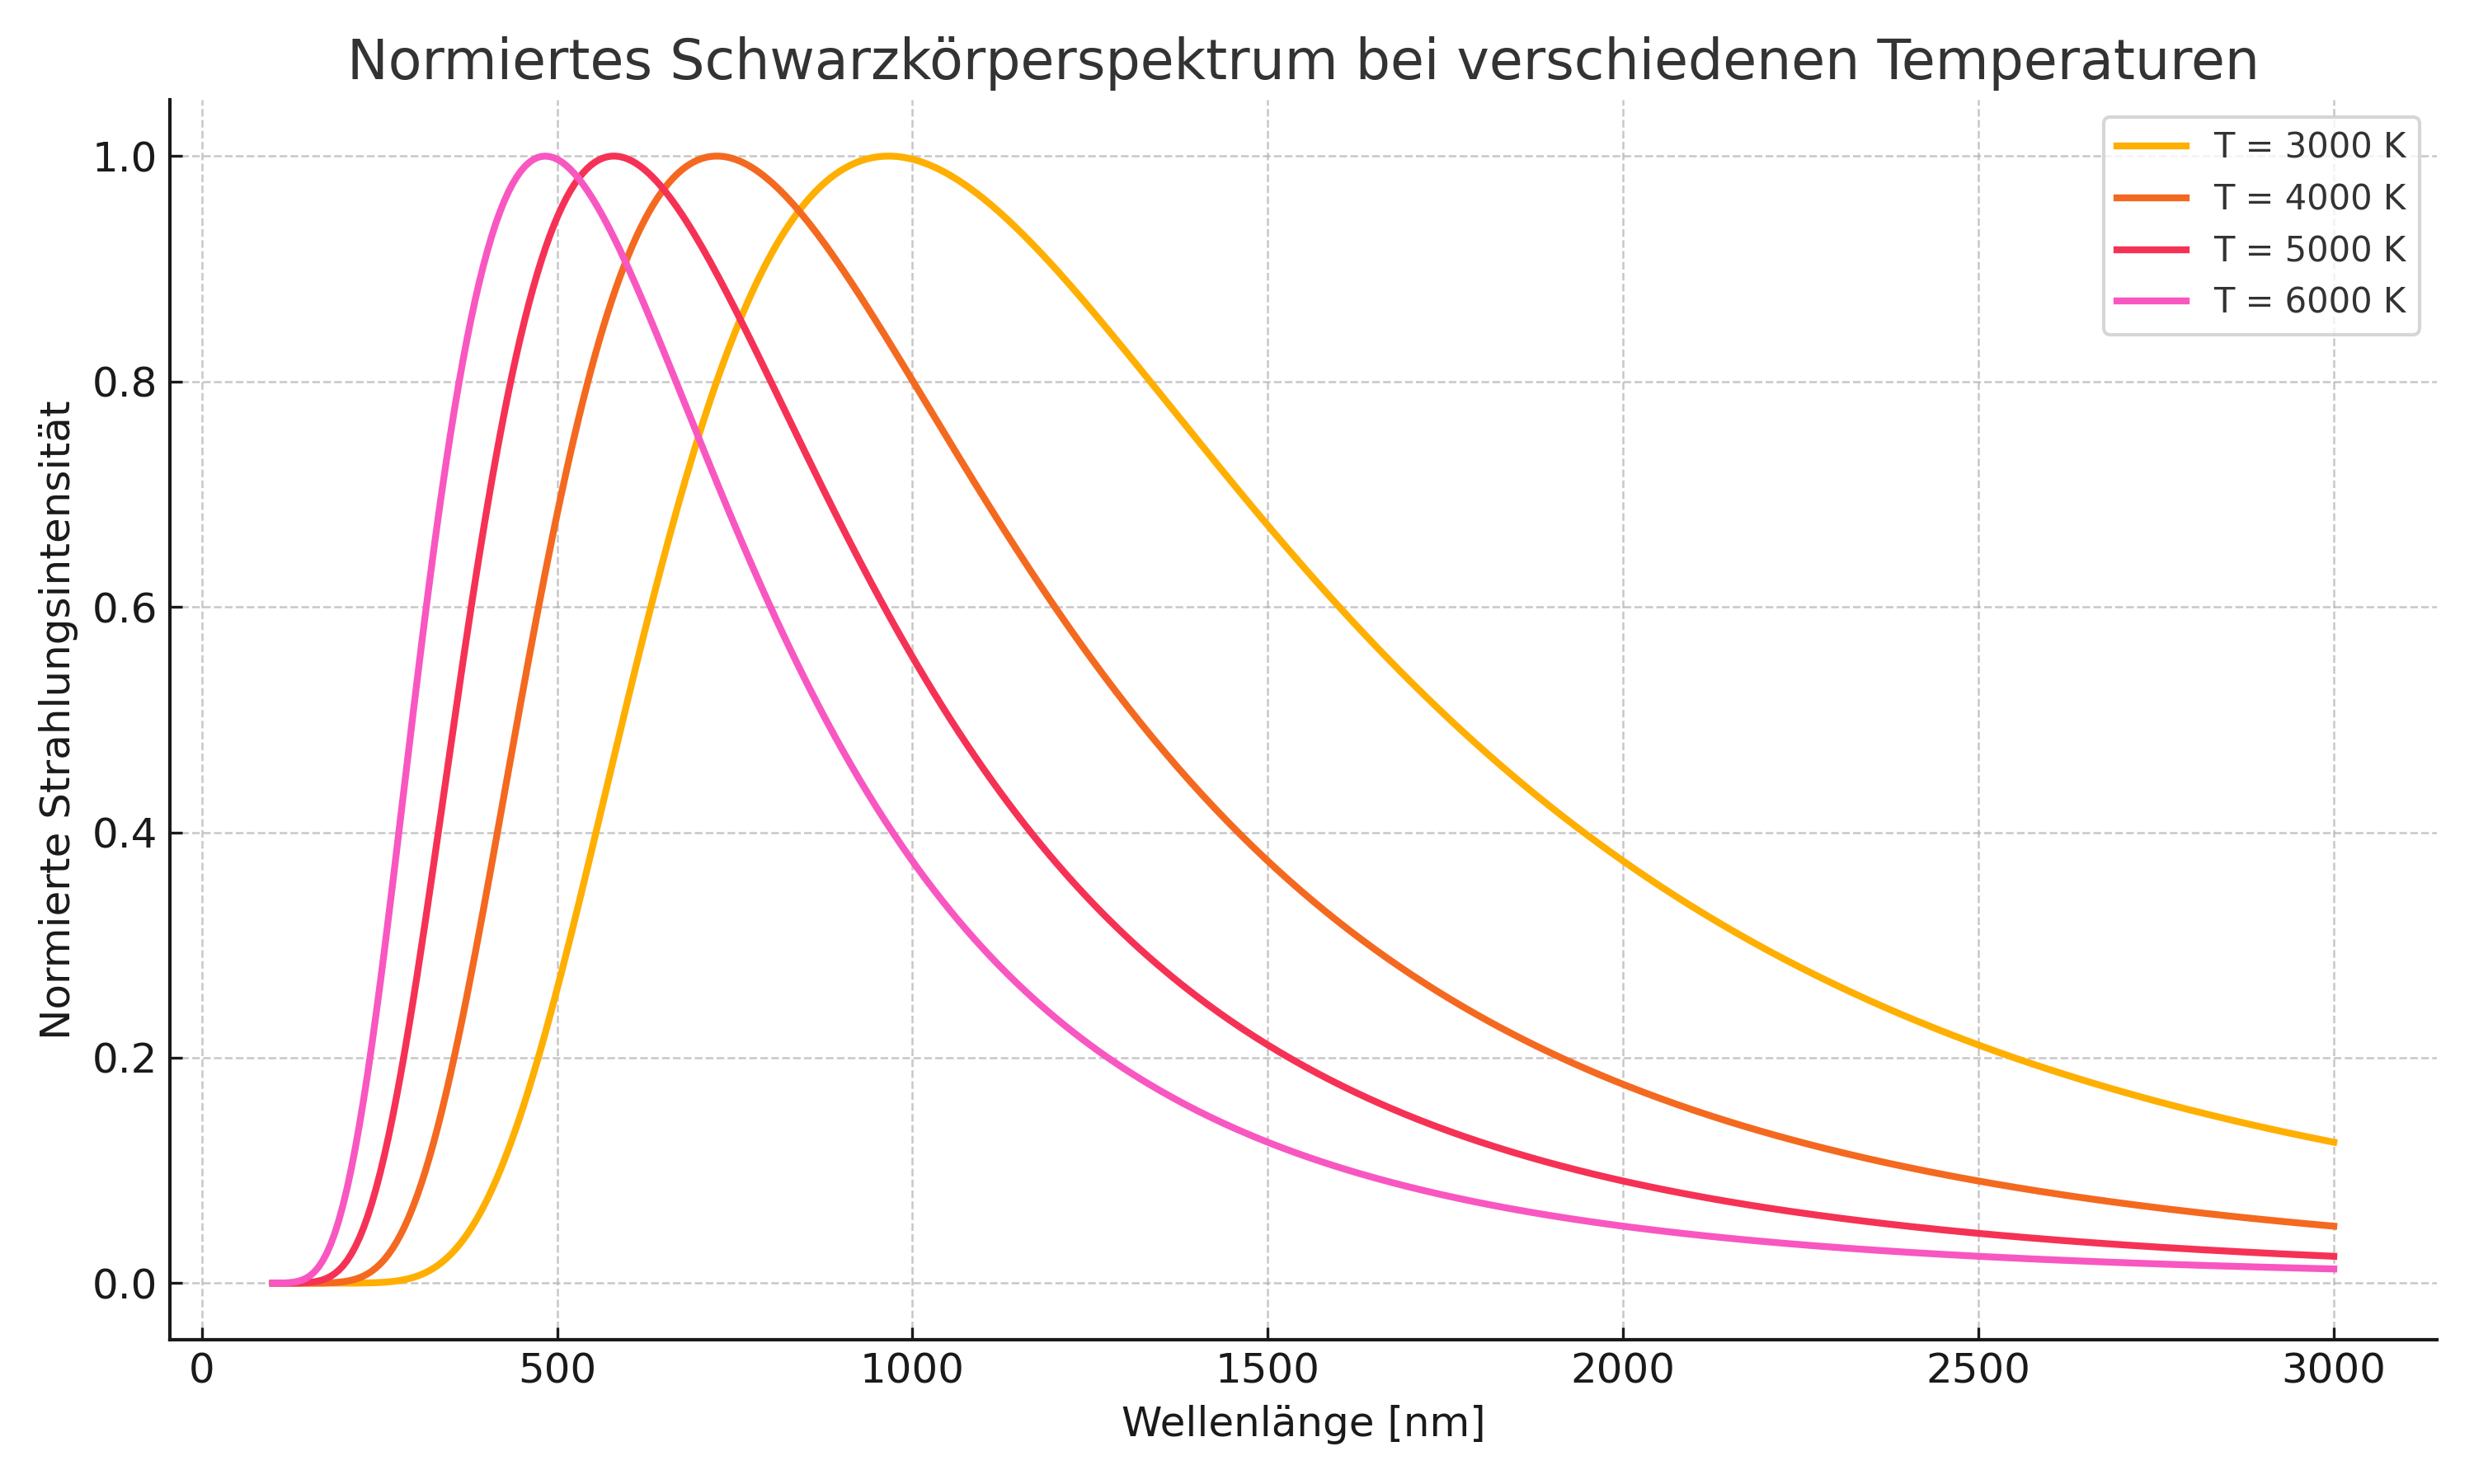
\includegraphics[width=0.85\textwidth]{bilder/schwarzer_koerper_spektrum.png}
	\caption{Normalized blackbody spectrum for different temperatures. The maximum shifts to shorter wavelengths as the temperature increases (Wien’s displacement law).}
	\label{fig:schwarzerkoerper}
\end{figure}
\subsubsection{Procedure of the Cavity Experiment}

To experimentally investigate thermal radiation, so-called \emph{cavity radiators}\index{Cavity Radiator} are used. They serve as nearly ideal realizations of a blackbody. The typical setup consists of a solid metal block with an inner cavity and a small opening to the outside world.

Radiation entering through this opening is reflected many times at the walls and is almost completely absorbed. Conversely, a tiny portion of the internal equilibrium radiation exits through the opening – this corresponds almost exactly to the theoretical blackbody radiation at the block’s temperature \( T \).  

The radiation emerging from the opening is studied with a spectrometer.\index{Spectrometer} The resulting spectrum shows the typical blackbody curve: an intensity profile with a maximum that shifts with temperature (Wien’s displacement law), and a characteristic drop in the ultraviolet region. These results fundamentally contradicted classical physics and ultimately led to the development of quantum theory.

\begin{figure}[H]
	\centering
	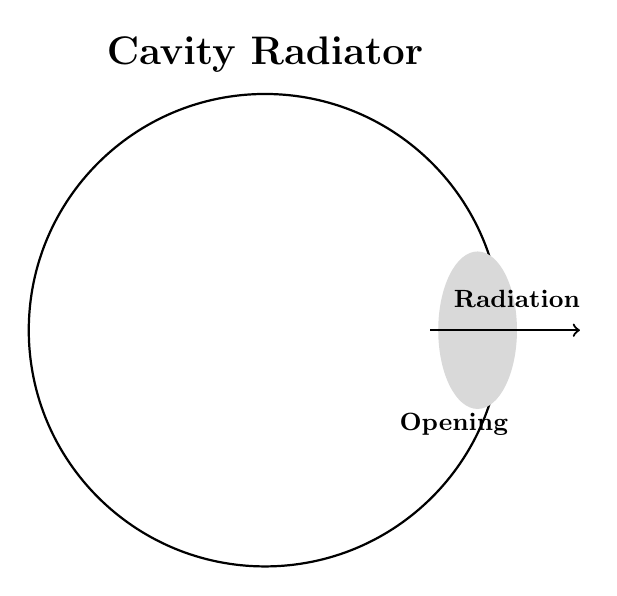
\begin{tikzpicture}
		% Cavity
		\draw[thick] (0,0) circle(3);
		% Opening (right side)
		\fill[gray!30] (2.7,0) ellipse (0.5 and 1.0);
		% Outgoing radiation
		\draw[->, thick] (2.1,0) -- (4,0);
		\node at (3.2,0.4) {\small \textbf{Radiation}};
		% Labels
		\node at (2.4,-1.2) {\small \textbf{Opening}};
		\node at (0,3.5) {\Large \textbf{Cavity Radiator}};
	\end{tikzpicture}
	\caption{Model of a cavity radiator producing nearly ideal blackbody radiation.}
\end{figure}
\subsection{Failure of the Classical Theory – \newline the Rayleigh–Jeans Law}\index{Rayleigh–Jeans Law}

In the 19th century, Lord Rayleigh and Sir James Jeans\index{Rayleigh, Lord}\index{Jeans, James} attempted to describe blackbody radiation using classical electrodynamics and statistical mechanics.\index{Statistical Mechanics} They treated standing electromagnetic waves in a cavity as harmonic oscillators and calculated the energy distribution by applying the equipartition principle of classical thermodynamics.\index{Equipartition Principle}
\newpage
\noindent
The result was the so-called \emph{Rayleigh–Jeans Law}, which gives the spectral energy density as a function of wavelength \( \lambda \) and temperature \( T \):

\[
u(\lambda, T) = \frac{8 \pi k T}{\lambda^4}
\]

Here:
\begin{itemize}
	\item \( u(\lambda, T) \): radiation energy per wavelength interval and volume,
	\item \( k \): Boltzmann constant,\index{Boltzmann Constant}
	\item \( T \): absolute temperature.
\end{itemize}

For long wavelengths the formula yields reasonable results and agrees well with experimental data. But at short wavelengths the expression diverges to infinity – leading to an unphysical, infinite energy density:

\[
\lim_{\lambda \to 0} u(\lambda, T) \to \infty
\]

This problem became known as the \emph{ultraviolet catastrophe}.\index{Ultraviolet Catastrophe} It stood in fundamental contradiction to experimental observations (see Fig.~\ref{fig:schwarzerkoerper}), where radiation in the UV region does not increase but instead falls off sharply.

This catastrophe revealed the limitations of classical physics. A new idea was required to explain the observations – and it came from Max Planck.  
(The derivation via mode counting in a cavity and the classical equipartition principle is presented in Appendix~A, Section~\ref{anhangA:rayleigh}.)
\subsection{Failure of the Classical Theory – \newline Wien’s Radiation Law}\index{Wien’s Radiation Law}

Even before Planck, Wilhelm Wien\index{Wien, Wilhelm} in 1896 provided an approximation for the radiation spectrum of blackbodies in the short-wavelength range. He derived the so-called \emph{Wien’s Radiation Law} from thermodynamic arguments and dimensional analysis – but without the quantum concept we know today.
\newpage
\noindent
The spectral energy density in wavelength form is given by:

\[
u(\lambda, T) = \frac{c_1}{\lambda^5} \exp\left(-\frac{c_2}{\lambda T}\right)
\]

with:
\begin{itemize}
	\item \( u(\lambda, T) \): energy per wavelength interval and volume,
	\item \( \lambda \): wavelength,\index{Wavelength}
	\item \( T \): absolute temperature,
	\item \( c_1 = 2\pi h c^2 \), \( c_2 = \tfrac{hc}{k} \): constants from Planck units (fully understood only later).\index{Planck Units}
\end{itemize}

Wien’s law describes the radiation distribution in the high-frequency range (\( \lambda \to 0 \)) very well and predicts an exponential decrease in intensity. In the long-wavelength range (\( \lambda \gg 1\ \mu\mathrm{m} \)), however, it deviates significantly from the measurements.

Wilhelm Wien received the Nobel Prize in 1911 for his contributions to radiation theory. His law was an important step toward Planck’s complete theory.  
(The mathematical derivation of Wien’s radiation law is given in Appendix~A; see Section~\ref{anhangA:wien}.)

\vspace{1em}
\begin{tcolorbox}[didaktikbox, title=Why Does the Classical Theory Fail?]
	\label{box:klassik-versagt}
	The Rayleigh–Jeans law correctly describes thermal radiation at low frequencies – but at high frequencies it gives absurd results:
	
	\begin{itemize}
		\item Intensity rises without bound – the higher the frequency, the greater the radiation.
		\item This “ultraviolet catastrophe” contradicts all observations.
		\item The cause: classical physics assumes that every mode in the cavity can absorb unlimited energy.
	\end{itemize}
	
	This assumption fails in reality. Only the quantization of energy – as introduced by Planck – explains why high frequencies are suppressed.
\end{tcolorbox}
\subsection{Emergence of Planck’s Radiation Law}\index{Planck’s Radiation Law}

At the end of the 19th century, describing the radiation of a blackbody posed a fundamental problem for theoretical physics. Empirically, the spectral energy density \( I(\lambda, T) \) was well known, but no theory could correctly explain the entire spectrum.

\subsubsection{The Crisis of Classical Physics}

Classical physics could only explain limiting cases:

\begin{itemize}
	\item For large wavelengths (\(\lambda \to \infty\)), the \textbf{Rayleigh–Jeans law}\index{Rayleigh–Jeans Law} was valid:
	\[
	I(\lambda, T) = \frac{8\pi c}{\lambda^4} \cdot kT
	\]
	This law, however, led to an unphysical divergence at short wavelengths – the so-called \textbf{ultraviolet catastrophe}.\index{Ultraviolet Catastrophe}
	
	\item For short wavelengths (\(\lambda \to 0\)), the \textbf{Wien’s law}\index{Wien’s Radiation Law} was known:
	\[
	I(\lambda, T) = c_1 \lambda^{-5} \cdot e^{-c_2/(\lambda T)}
	\]
	Yet it failed in the long-wavelength region.
\end{itemize}

\subsubsection{Planck’s Interpolation Approach}

Max Planck\index{Planck, Max} was familiar with both limiting laws and searched for a mathematical function that could interpolate across the entire observed curve. In October 1900, this led him to his famous formula:
\begin{align}
	I(\lambda, T) = \frac{2hc^2}{\lambda^5} \cdot \frac{1}{e^{hc/(\lambda kT)} - 1}
\end{align}

with:
\begin{itemize}
	\item \( h \): Planck’s constant\index{Planck’s Constant}
	\item \( c \): speed of light\index{Speed of Light}
	\item \( k \): Boltzmann constant\index{Boltzmann Constant}
	\item \( T \): absolute temperature
\end{itemize}

(The detailed derivation of Planck’s radiation law using energy quantization is presented in Appendix~A, Section~\ref{anhangA:planck}.)

\subsubsection{Remark on the Meaning of \( h \)}

Planck initially regarded his formula as a \textbf{mathematical interpolation}, not as the expression of a fundamental natural constant. He introduced \( h \) to fit the curve – without realizing the revolutionary consequences. Only Albert Einstein\index{Einstein, Albert} recognized its deeper meaning in 1905 within the framework of his light quantum hypothesis.

\vspace{-0.3em}
\begin{tcolorbox}[physikbox,title={Max Planck – Scientific Autobiography \cite{Planck1948}}]
	\label{box:planck-zitat}
	“I had the feeling that I had introduced something monstrous against my will.”
\end{tcolorbox}

\vspace{1em}
\begin{tcolorbox}[mathebox, title={Planck’s Radiation Law: A Mathematical Interpolation \cite{Hoffmann2008}}]
	\label{box:planck-interpolation}
	At the end of 1900, Max Planck was searching for a function to correctly describe the observed blackbody radiation curves. He combined known limiting laws (Wien for high, Rayleigh for low frequencies) and developed an interpolation formula that later became known as Planck’s radiation law:
	
	\begin{align}
		I(\nu, T) = \frac{8\pi \nu^2}{c^3} \cdot \frac{h\nu}{e^{h\nu/kT} - 1}
	\end{align}
	
	At the time, he himself was unaware of the deeper meaning of the constant \( h \) – for him it was a mathematical tool. Only later did Einstein, with his light quantum hypothesis of 1905, interpret this formula as evidence of a fundamental quantization of nature.
\end{tcolorbox}
\newpage
\noindent
\subsubsection{Important Historical Insight}
\vspace{1em}
\begin{tcolorbox}[didaktikbox,title=Important Historical Insight {\cite{Hoffmann2008}}]
	\label{box:geschichte-planck}
	On December 14, 1900, Max Planck presented his famous radiation formula to the Physical Society. Today this day is regarded as the \textit{“birthday of quantum physics”}. Yet neither Planck nor his audience recognized the significance of the discovery at the time.
	
	\medskip
	\textbf{Quote:} 
	\begin{quote}
		“Although none of the scientists present – including Planck himself – were aware of the meaning and scope of the formula or the constant. Planck’s result was initially seen merely as a formula that correctly represented the radiation data.”
	\end{quote}
	
	As Hoffmann points out, the revolution only became clear through Einstein’s light quantum hypothesis (1905) and the critical analysis of Planck’s law by Einstein and Ehrenfest. Planck himself spoke of a fundamental upheaval only years later.
\end{tcolorbox}
\index{Quantum Physics}
\newpage
\noindent
\subsubsection{Graphical Comparison of the Three Radiation Laws}

The following figure shows the spectral energy density of blackbodies as a function of wavelength. It compares the classical Rayleigh–Jeans law, Wien’s radiation law, and the full Planck law. The diagram clearly illustrates:

\begin{itemize}
	\item The Rayleigh–Jeans law diverges in the UV region.
	\item Wien’s law is valid only in the short-wavelength region.
	\item Only Planck’s law correctly describes the entire spectrum.
\end{itemize}

\begin{figure}[H]
	\centering
	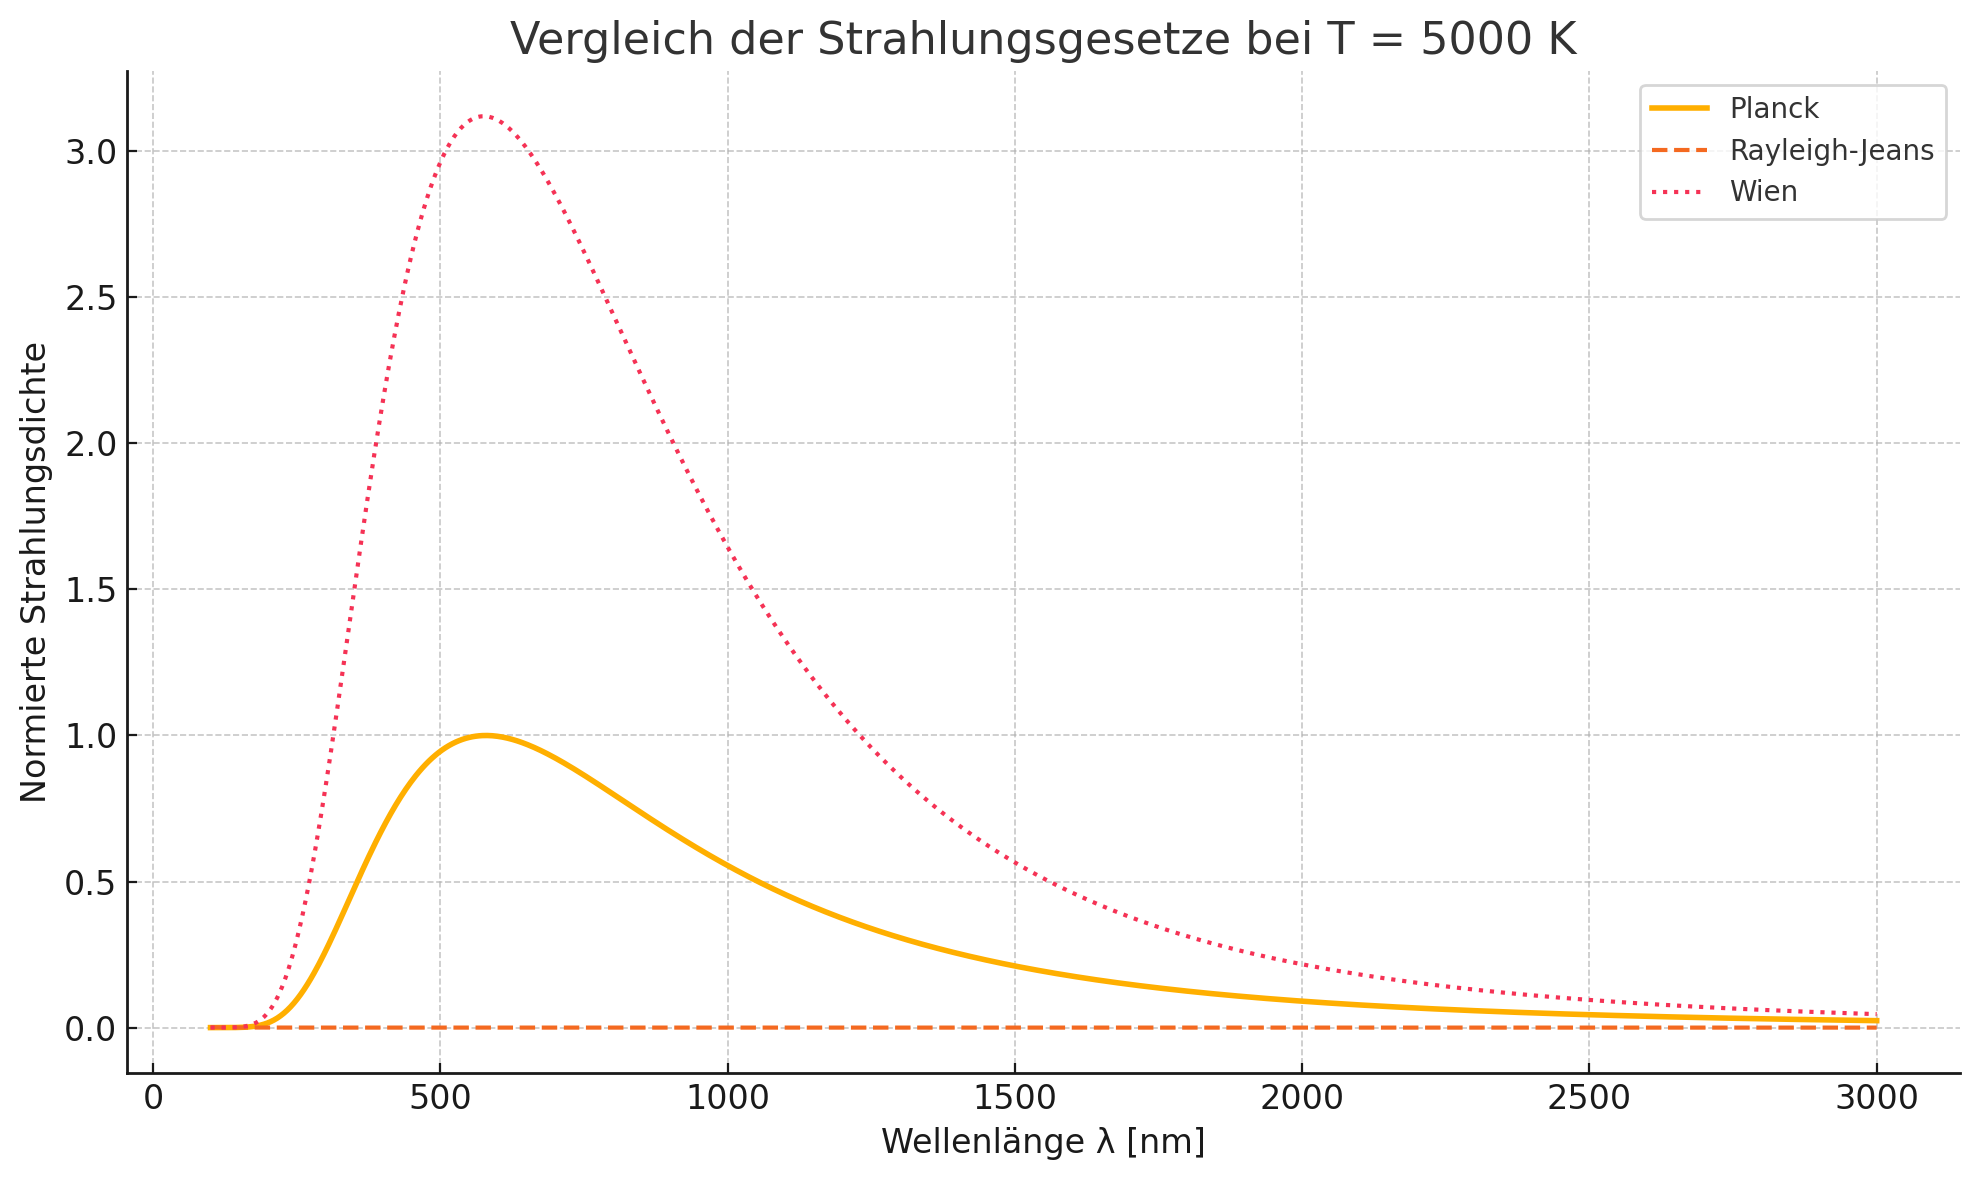
\includegraphics[width=0.85\textwidth]{bilder/strahlungsgesetze.png}
	\caption{Comparison of the three radiation laws. Only Planck’s law agrees with experimental data across the entire spectrum.}
	\label{fig:strahlungsgesetze}
\end{figure}

\subsubsection{Conclusion}

\begin{itemize}
	\item The error of the classical theory is not only large but catastrophic.
	\item The deviation at short wavelengths amounts to several orders of magnitude.
	\item Only Planck’s law explains the entire spectrum correctly – by quantizing energy.
\end{itemize}
\subsection{The Photoelectric Effect and Einstein’s Light Quantum}\index{Photoelectric Effect}

In 1905, Einstein went a step further: not only the emission of energy, but light itself was quantized. He postulated that a light quantum (photon) carries the energy \( E = h\nu \).\index{Einstein, Albert} Only if this energy exceeds the work function \( A \) can an electron be emitted:  
\[
E_{\text{kin}} = h\nu - A
\]
This explained experimental observations that were incompatible with the wave theory – in particular the frequency dependence of the electron energies.\index{Work Function}

\begin{tcolorbox}[physikbox, title={Einstein (1905)\cite{einstein_lichtquanten}}]
	\label{box:einstein-lichtquant}
	“The generation of light does not occur everywhere along the wavefront uniformly, but only at certain places, at individual points.”
	
	\textbf{Comment:} Here Einstein already describes the quantization of light – the starting point of photon theory.
\end{tcolorbox}
\vspace{1em}
\index{Light Quantum Hypothesis}

(A detailed derivation of the photoelectric equation can be found in Appendix~A, Section~\ref{anhangA:photoeffekt}.)
\subsection{First Reactions and Significance}

The idea that light possesses not only wave properties but also particle properties was difficult for many physicists at the beginning of the 20th century to accept. The wave theory of light had seemed fully confirmed by interference and diffraction experiments as well as by Maxwell’s electrodynamics.\index{Wave Theory of Light} Albert Einstein’s light quantum theory of 1905 – the radical thesis that light consists of discrete energy packets (later called \emph{photons}) – contradicted this established view.

Einstein himself was aware of the explosive nature of his hypothesis and described it as a “heuristic point of view.” Yet the concept was more than a mere computational trick – it fully explained the photoelectric effect and led to precise, experimentally testable predictions.

A striking example of the initial skepticism was Robert A. Millikan.\index{Millikan, Robert A.} Although in 1916 he himself confirmed the energy formula \( E = h \nu \) with high precision in a series of experiments, he long remained critical of the light quantum concept:

Only decades later did the light quantum hypothesis become accepted as a fundamental part of quantum physics – especially after phenomena such as \emph{Compton scattering} (1923) confirmed the momentum nature of the photon.\index{Compton Scattering}


The introduction of the photon revolutionized not only optics but was also crucial for:
\begin{itemize}
	\item the development of \emph{quantum mechanics},\index{Quantum Mechanics}
	\item the understanding of \emph{atoms and molecules},\index{Atom}\index{Molecule}
	\item the theory of \emph{quantum electrodynamics (QED)},\index{Quantum Electrodynamics (QED)}
	\item as well as numerous \emph{technological applications} (lasers, photodetectors, solar cells, quantum computers).\index{Laser}\index{Photodetector}\index{Solar Cell}\index{Quantum Computer}
\end{itemize}

Today the photon is not merely a theoretical construct, but a real object, demonstrated in countless experiments and used in technology – a \emph{quantum of the electromagnetic interaction}.\index{Electromagnetic Interaction}

\vspace{1em}
\begin{tcolorbox}[physikbox, title=Robert A. Millikan on Einstein (1916) \cite{millikan_1916}]
	\label{box:millikan-einstein}
	\emph{“Einstein’s photoelectric equation … cannot in my judgment be looked upon at present as resting upon a satisfactory theoretical foundation.”}
	
	\vspace{6pt}
	\textbf{Comment:} Despite his experimental confirmation of Einstein’s formula, Millikan initially rejected the light quantum concept – a striking example of how deeply rooted theoretical convictions cannot be immediately overturned, even by clear experimental evidence.
\end{tcolorbox}
\subsection{Conclusion}
\vspace{1em}
\begin{tcolorbox}[hypobox, title={What If There Were No Quantization?}]
	\label{box:hypo-keine-quanten}
	Without the assumption that energy can only be absorbed or emitted in discrete portions ($E = nhf$):\index{Quantization}
	\begin{itemize}
		\item Fundamental experiments such as blackbody radiation and the photoelectric effect would have remained unexplained.
		\item Classical physics would have collapsed under the contradictions with reality.
		\item No modern understanding of the interaction between light and matter would have developed.
	\end{itemize}
	Quantization was the first step toward a new physical worldview. It is not optional – it is essential for understanding the photon.
\end{tcolorbox}


	\chapter{Properties of the Photon}\index{Photon}\index{Quantum mechanics}\index{Quantum physics}

\setcounter{section}{3}
\setcounter{subsection}{0}
\setcounter{subsubsection}{1}
\setcounter{secnumdepth}{3}
% Define box styles
\tcbset{physikbox/.style={colback=blue!5!white, colframe=blue!75!black, fonttitle=\bfseries}}
\tcbset{mathebox/.style={colback=green!5!white, colframe=green!50!black, fonttitle=\bfseries}}
\tcbset{didaktikbox/.style={colback=yellow!5!white, colframe=yellow!50!black, fonttitle=\bfseries}}
\tcbset{hypobox/.style={colback=orange!5!white, colframe=orange!75!black, fonttitle=\bfseries}}
\tcbset{hinweisbox/.style={colback=gray!10!white, colframe=black!40!black, fonttitle=\bfseries}}

\subsection{Photons as Quanta of Energy}\index{Energy quantum}

The idea that energy does not exist continuously but in discrete portions – so-called quanta – was revolutionary at the beginning of the 20th century. The starting point, however, was not a deliberate physical revolution but a mathematical device introduced by Max Planck in 1900.\index{Planck, Max}

\subsubsection{Planck's Formula as a Makeshift Solution}

Planck attempted to correctly describe the radiation spectrum of a black body. To achieve this, he formally introduced a quantization of energy.\index{Quantization} He assumed that the energy elements absorbed or emitted by hypothetical oscillators must be integer multiples of a smallest unit of energy of the form
$$
\varepsilon = h \nu
$$

with:
\begin{itemize}
	\item $\varepsilon$: energy of an oscillator,
	\item $\nu$: its oscillation frequency,\index{Frequency}
	\item $h$: the Planck constant, $h \approx 6.626 \cdot 10^{-34}~\mathrm{Js}$.\index{Planck constant}
\end{itemize}

Planck himself did not regard this assumption as a statement about reality, but as a mathematical–statistical device for deriving the radiation law \cite{planck1948}. In his \emph{Scientific Autobiography} he wrote in retrospect:
\newpage
\noindent
\begin{tcolorbox}[physikbox, title={Max Planck (1905)\cite{planck1948}}]
	\label{box:planck1948}
	“I had resolved to derive the radiation formula at any cost, and I accomplished this, no matter what it took. [...] The introduction of an elementary quantum of action was a purely formal assumption – I did not at all intend to introduce a physical quantum theory.”
\end{tcolorbox}
\index{Planck, Max}

\subsubsection{Einstein Turns Them into Light Quanta}

It was \textbf{Albert Einstein} who realized in 1905, in his work on the photoelectric effect, that quantization might not merely be a calculational trick, but a real property of light.\index{Einstein, Albert}\index{Photoelectric effect} He postulated that light consists of discrete packets of energy – later called \emph{photons}. The energy of such a photon is given by:
$$
E = h \nu
$$
This laid the foundation of quantum theory \cite{einstein1905}.\index{Quantum theory}

\subsubsection{Examples from Different Frequency Ranges}

The energy of a photon depends only on its frequency $\nu$ (or equivalently its wavelength $\lambda$) – independent of light intensity.\index{Wavelength}\index{Light intensity} This is impressively demonstrated by typical examples from nature and technology:

\subsubsection*{Green Light}
\phantomsection
Given the frequency of typical green light:
$$
\nu = 6.0 \cdot 10^{14}~\mathrm{Hz}
$$
The wavelength follows from:
$$
\lambda = \frac{c}{\nu}
$$
with the speed of light \( c = 3.0 \cdot 10^8~\mathrm{m/s} \).\index{Speed of light} Thus:
$$
\lambda = \frac{3.0 \cdot 10^8~\mathrm{m/s}}{6.0 \cdot 10^{14}~\mathrm{Hz}} = 5.0 \cdot 10^{-7}~\mathrm{m} = 500~\mathrm{nm}
$$
Now we compute the energy of a single photon:
$$
E = h \cdot \nu = 6.626 \cdot 10^{-34}~\mathrm{Js} \cdot 6.0 \cdot 10^{14}~\mathrm{Hz} = 3.976 \cdot 10^{-19}~\mathrm{J}
$$
This tiny amount of energy is sufficient to trigger a chemical reaction in the retina of the eye – the beginning of vision.
\vspace{1em}

\begin{tcolorbox}[physikbox, title=Green Light]
	\label{box:grünesLicht}
	A photon of green light with \( \nu = 6 \cdot 10^{14}~\mathrm{Hz} \) has a wavelength of \( \lambda = 500~\mathrm{nm} \) and an energy of about \( 4 \cdot 10^{-19}~\mathrm{J} \).
\end{tcolorbox}
\index{Visible light}

\subsubsection*{X-Rays}
\phantomsection
X-radiation has an extremely high frequency and correspondingly short wavelength (in the range of tenths of a nanometer).\index{X-rays} A single photon carries much more energy than visible light – enough to eject electrons from inner atomic shells. This is the physical basis of medical X-ray imaging – but also the reason why such radiation is biologically effective and potentially harmful.
\vspace{1em}
\begin{tcolorbox}[physikbox, title=X-Rays]
	\label{box:röntgenstrahlen}
	An X-ray photon with \( \nu = 3 \cdot 10^{18}~\mathrm{Hz} \) has a wavelength of about \( \lambda = 0.1~\mathrm{nm} \) and an energy of about \( 2 \cdot 10^{-15}~\mathrm{J} = 12.4~\mathrm{keV} \).
\end{tcolorbox}

\subsubsection*{Microwaves}
\phantomsection
Microwaves have very low frequencies and correspondingly long wavelengths – typically several centimeters.\index{Microwave} A single photon carries very little energy. It is insufficient to remove electrons or directly trigger chemical reactions, but it is just right to excite water molecules in food into motion. This generates heat – the physical principle behind microwave ovens.
\vspace{1em}
\begin{tcolorbox}[physikbox, title=Microwaves]
	\label{box:Mikrowellenstrahlung}
	A photon of typical microwave radiation with \( \nu = 2.45 \cdot 10^9~\mathrm{Hz} \) has a wavelength of about \( \lambda = 1.22\cdot 10^8~\mathrm{nm} \)
	and an energy of about \( 1.62 \cdot 10^{-24}~\mathrm{J} \).
\end{tcolorbox}
\newpage
\noindent
\subsubsection{Summary}

\begin{tcolorbox}[mathebox,title=Photons as Quanta of Energy]
	\label{box:Photon als Energiequanten}
	The equation $E = h \nu$ was originally a mathematical device for describing blackbody radiation \cite{planck1948}. Only in 1905 did Einstein realize that it describes the real nature of light: light consists of discrete packets of energy – photons \cite{einstein1905}. This marked the beginning of quantum theory.
\end{tcolorbox}
\index{Blackbody radiation}
\index{Einstein, Albert}

\subsection{Momentum of the Photon}\index{Momentum}

An essential feature of the photon is its momentum – even though it has no rest mass.\index{Rest mass} In classical mechanics, the momentum of a particle is defined as the product of mass and velocity:
$$
p = m \cdot v
$$
Because photons are massless \((m_0 = 0)\), this relation seems inapplicable at first sight. Nevertheless, photons carry momentum – a fact spectacularly confirmed by experiments such as Compton scattering.\index{Compton scattering} The explanation is provided by quantum physics in conjunction with special relativity.\index{Special relativity}

\subsubsection{Momentum from the Quantization of Light}

The energy of a photon is, according to Planck and Einstein,
$$
E = h \cdot \nu
$$

At the same time, special relativity gives for massless particles like the photon:
$$
E = p \cdot c
$$
Equating both expressions yields the photon momentum:
$$
p = \frac{E}{c} = \frac{h \cdot \nu}{c}
$$
Since frequency and wavelength are related by \(\nu = \tfrac{c}{\lambda}\), we obtain
$$
p = \frac{h}{\lambda} \quad \text{(III.3)}
$$
(A formal derivation via the relativistic energy–momentum relation is given in Appendix~A; see Sec.~\ref{anhangA:impuls}.)

This expression shows: The momentum of a photon is inversely proportional to its wavelength – the shorter the wavelength, the larger the momentum.
\vspace{1em}
\begin{tcolorbox}[physikbox,title=Photon Momentum]
	\label{box:Photonenimpuls}
	A photon has momentum
	$$
	p = \frac{h}{\lambda}
	$$
	despite having no rest mass. The momentum increases with increasing frequency or decreasing wavelength.
\end{tcolorbox}
\index{Photon momentum}

\subsubsection{Momentum Transfer in Practice}

That light carries momentum is evident, for example, from the radiation pressure exerted on matter – an effect already suspected by Kepler and later confirmed experimentally.\index{Radiation pressure}

In modern technology, photon momentum plays a role in, for example:
\begin{itemize}
	\item \textbf{Solar sails:} using radiation pressure to propel spacecraft.\index{Solar sail}
	\begin{tcolorbox}[hinweisbox, title=Real-World Image Material]
		\label{keybox:RealesBildmaterial}
		A real photo of the deployed solar sail of the \textbf{IKAROS} spacecraft was taken in 2010 by the mini camera \textbf{DCAM2}.  
		You can find it online at The Planetary Society:  
		\url{https://www.planetary.org/space-images/ikaros-spacecraft-from-dcam2}
	\end{tcolorbox}
	\item \textbf{Optical tweezers:} manipulation of small particles with focused light beams.\index{Optical tweezers}
	\begin{tcolorbox}[hinweisbox, title=Image Material for Optical Tweezers]
		\label{box:Manipulation kleiner Partikel}
		A real image and schematic of optical tweezers (laser trap) is publicly available on Wikipedia:  
		\url{https://en.wikipedia.org/wiki/Optical_tweezers}
	\end{tcolorbox}
\end{itemize}

\subsubsection{Connection to the de Broglie Wavelength}

The expression \( p = \tfrac{h}{\lambda} \) is not limited to photons; it also holds for matter waves (the de Broglie relation).\index{de Broglie relation} For massive particles:
$$
\lambda = \frac{h}{p}
$$
This links wave character and momentum – another confirmation of wave–particle duality also for light.\index{Wave–particle duality}

\subsection{Health Aspects of Electromagnetic Radiation}\index{Electromagnetic radiation}\index{Health}

\subsubsection{Ionizing Radiation: UV Light and Beyond}

Ultraviolet radiation, especially below \SI{280}{\nano\meter}, has photons with energies of several \si{\electronvolt}. These are sufficient to remove electrons from atoms or to break chemical bonds – this is \textbf{ionizing radiation}.\index{Ionizing radiation}\index{Ultraviolet}

$$
E = h\nu = \frac{hc}{\lambda}
$$

For UV light with \(\lambda = \SI{200}{\nano\meter}\),
$$
E = \frac{6.626 \cdot 10^{-34}\,\si{\joule\second} \cdot 3.0 \cdot 10^8\,\si{\meter\per\second}}{200 \cdot 10^{-9}\,\si{\meter}}
= \SI{9.939e-19}{\joule} \approx \SI{6.2}{\electronvolt}
$$
This energy suffices to damage DNA molecules – a physical mechanism known to cause \textbf{skin cancer}.\index{DNA}\index{Skin cancer}

\subsubsection{Non-Ionizing Radiation: Mobile Networks, WLAN, Microwaves}

Radiation in the radio, WLAN, or microwave range has much lower photon energies:
\begin{itemize}
	\item Mobile networks: $\nu \approx \SI{900}{\mega\hertz} \Rightarrow E \approx \SI{3.7e-6}{\electronvolt}$
	\item WLAN: $\nu \approx \SI{2.4}{\giga\hertz} \Rightarrow E \approx \SI{1.0e-5}{\electronvolt}$
	\item Microwave: $\nu \approx \SI{2.45}{\giga\hertz} \Rightarrow E \approx \SI{1.01e-5}{\electronvolt}$
\end{itemize}
These energies are \textbf{not sufficient} to cause ionization.\index{Non-ionizing radiation} Nevertheless, there is discussion about thermal or biological effects through \textbf{cumulative energy absorption}.

\subsubsection{Summary – Ionizing vs. Non-Ionizing Radiation}
\vspace{1em}
\begin{tcolorbox}[physikbox,title=Ionizing and Non-Ionizing Radiation]
	\label{box:ionisierende}
	\begin{itemize}
		\item \textbf{Non-ionizing:} photons have too little energy to remove electrons from atoms. Examples:
		\begin{itemize}
			\item Radio waves, microwaves
			\item Infrared, visible light
			\item Mobile networks, WLAN, Bluetooth
		\end{itemize}
		\item \textbf{Ionizing:} photons have enough energy to ionize atoms, potentially causing cell or DNA damage. Examples:
		\begin{itemize}
			\item Ultraviolet (especially UV-B, UV-C)
			\item X-rays
			\item Gamma rays
		\end{itemize}
	\end{itemize}
\end{tcolorbox}
\index{Radio waves}\index{Infrared}\index{Visible light}\index{X-rays}\index{Gamma rays}
\vspace{1em}

\subsubsection{Limits and Protective Measures}

In practice, safety limits are set to avoid excessive exposure. The key metric is the \textbf{Specific Absorption Rate (SAR)} measured in \si{\watt\per\kilogram}, describing how much electromagnetic energy per kilogram of body tissue is absorbed.\index{SAR (specific absorption rate)}

\begin{itemize}
	\item EU limit for mobile devices: \SI{2}{\watt\per\kilogram}
	\item WLAN routers: typically well below this
\end{itemize}

\subsubsection{Case Study: UV-C Radiation for Disinfection}

Ultraviolet radiation in the range \SI{200}{nm}–\SI{280}{nm} – so-called \textbf{UV-C} – has photon energies up to \SI{6.2}{\electronvolt}.\index{UV-C} This is sufficient to \textbf{directly damage DNA and RNA of microorganisms}, e.g., by forming pyrimidine dimers, thereby inhibiting their replication.
\newpage
\noindent
\textbf{Applications:}
\begin{itemize}
	\item Hospitals: UV-C lamps for disinfection of surfaces, air, and equipment.
	\item Drinking water treatment: UV-C without chemical additives.
\end{itemize}

\textbf{Physical basis:}
$$
E = \frac{hc}{\lambda} = \frac{6.626 \cdot 10^{-34}\,\si{\joule\second} \cdot 3.0 \cdot 10^8\,\si{\meter\per\second}}{254 \cdot 10^{-9}\,\si{\meter}} \approx \SI{7.83e-19}{\joule} \approx \SI{4.9}{\electronvolt}
$$
This energy suffices to break covalent bonds in DNA – a clear physical mechanism of disinfection.
\vspace{0.5em}
\begin{tcolorbox}[physikbox, title=Note on Hazard]
	\label{box:Hinweis zur Gefärdung}
	UV-C affects not only microorganisms but can also damage human skin and eyes. Direct exposure must be strictly avoided.
\end{tcolorbox}
\newpage
\noindent
\subsection{The Electromagnetic Spectrum}\index{Electromagnetic spectrum}

\subsubsection{Overview}

The electromagnetic spectrum encompasses all forms of electromagnetic radiation – from long-wavelength radio waves to short-wavelength gamma rays. One typically distinguishes by frequency \(\nu\), wavelength \(\lambda\), or photon energy \(E = h\nu = \tfrac{hc}{\lambda}\).

\subsubsection{Representation}

\begin{figure}[H]
	\centering
	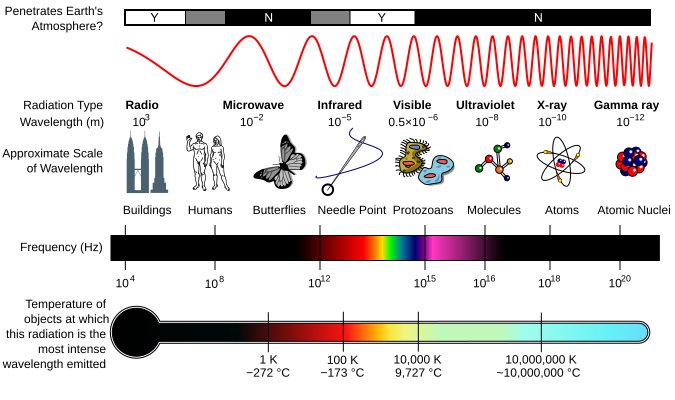
\includegraphics[width=\textwidth]{bilder/spektrum.png}
	\caption{The electromagnetic spectrum with typical applications. Source: Wikimedia Commons}
	\label{fig:em_spektrum}
\end{figure}

\subsubsection{Frequency, Wavelength, and Energy Ranges}

\begin{table}[H]
	\centering
	\scriptsize
	\resizebox{0.95\textwidth}{!}{
		\begin{tabular}{|l|c|c|c|}
			\hline
			\textbf{\raisebox{-0.2ex}{Region}} & \textbf{\raisebox{-0.2ex}{Frequency}} & \textbf{\raisebox{-0.2ex}{Wavelength}} & \textbf{\raisebox{-0.2ex}{Photon energy}} \\
			\hline
			Radio waves      & \SI{1e3}{}–\SI{1e8}{Hz} & km – m & \(\sim\)\SI{1e-9}{eV} \\
			Microwaves       & \SI{1e8}{}–\SI{1e11}{Hz} & m – mm & \(\sim\)\SI{1e-6}{eV} \\
			Infrared         & \SI{1e11}{}–\SI{4e14}{Hz} & mm – \SI{750}{nm} & \SI{1e-3}{eV} – \SI{1}{eV} \\
			Visible light    & \SI{4e14}{}–\SI{8e14}{Hz} & \SI{750}{nm} – \SI{380}{nm} & \SI{1.6}{eV} – \SI{3.3}{eV} \\
			Ultraviolet      & \SI{8e14}{}–\SI{3e16}{Hz} & \SI{380}{nm} – \SI{10}{nm} & up to \SI{100}{eV} \\
			X-rays           & \SI{3e16}{}–\SI{3e19}{Hz} & \SI{10}{nm} – \SI{0.01}{nm} & \SI{100}{eV} – \SI{100}{keV} \\
			Gamma rays       & >\SI{3e19}{Hz} & < \SI{0.01}{nm} & > \SI{100}{keV} \\
			\hline
		\end{tabular}
	}
	\caption{Typical regions of the electromagnetic spectrum with frequency, wavelength, and energy}
	\label{tab:spektrum}
\end{table}

\subsubsection{Applications Across the Spectrum}

Typical applications in different spectral regions:
\begin{itemize}
	\item \textbf{Radio waves:} broadcasting, radio communication, MRI
	\item \textbf{Microwaves:} mobile networks, WLAN, microwave oven
	\item \textbf{Infrared:} remote controls, thermography
	\item \textbf{Visible:} optics, photography, biological vision
	\item \textbf{UV:} sunburn, disinfection (UV-C)
	\item \textbf{X-ray:} medical imaging, materials testing
	\item \textbf{Gamma:} radiation therapy, astrophysics
\end{itemize}

\begin{tcolorbox}[hinweisbox,title=Takeaways on the Electromagnetic Spectrum]
	\label{box:Fazit zum elektro}
	\textbf{Physical takeaways:}
	\begin{itemize}
		\item The electromagnetic spectrum spans waves of all frequencies – from radio to gamma.
		\item Photon energy increases with increasing frequency (or decreasing wavelength) according to \(E = h \nu = \tfrac{hc}{\lambda}\).
		\item The transition to \textbf{ionizing radiation} typically begins in the UV, at photon energies around \SI{10}{\electronvolt}.
	\end{itemize}
	\vspace{0.5em}
	\textbf{Didactic takeaways:}
	\begin{itemize}
		\item Placing typical applications – e.g., mobile networks, microwaves, UV disinfection, X-ray diagnostics – in the spectrum clarifies their physical and biological effects.
		\item A visual link between frequency, wavelength, energy, and biological relevance is especially helpful.
		\item \textbf{Rule of thumb:} the shorter the wavelength, the higher the photon energy – and the greater the potential for biological damage.
	\end{itemize}
\end{tcolorbox}
\newpage
\noindent

\subsection{Masslessness and Propagation at the Speed of Light}\index{Masslessness}\index{Speed of light}

\subsubsection{No Rest Mass – Yet Energy and Momentum}

The photon has no rest mass, i.e., $m_0 = 0$. Nevertheless, it carries energy and momentum.\index{Energy} The photon energy (Planck–Einstein) is
$$
E = h \nu
$$
and the momentum follows as
$$
p = \frac{E}{c} = \frac{h\nu}{c} = \frac{h}{\lambda}
$$
Thus the photon does not contradict relativity – on the contrary: these relations are direct consequences of special relativity for massless particles.

\subsubsection{What If the Photon Had a Tiny Mass?}

\paragraph{Relativistic energy:} If the photon were not exactly massless, one would have to use the general relativistic energy formula
$$
E = \gamma m_0 c^2 = \frac{m_0 c^2}{\sqrt{1 - \frac{v^2}{c^2}}}
$$
and the momentum
$$
p = \gamma m_0 v
$$
Then the simple relation $E = pc$ would no longer be exact; instead
$$
E^2 = (pc)^2 + (m_0 c^2)^2
$$
(A detailed mathematical discussion for massless and hypothetically massive photons is given in Appendix~A, Sec.~\ref{anhangA:masse}.)
\newpage
\noindent
\subsubsection*{Physical Consequences:}
\phantomsection
\begin{itemize}
	\item The speed of light would no longer be the same for all photons.
	\item The speed would depend on energy (frequency) $\Rightarrow$ violation of Lorentz invariance.
	\item Long-wavelength light would travel more slowly than short-wavelength light.
	\item Coulomb's law would have to be modified $\Rightarrow$ the range of the electric force would be finite.
\end{itemize}

\paragraph{Experimental Bounds:}
Precise measurements show: if the photon has a mass, it must be extremely small:
$$
m_\gamma < 10^{-54}~\text{kg} \approx 10^{-18}~\text{eV}/c^2
$$
\index{Photon mass}
\textbf{This number} $10^{-54}~\text{kg}$ \textbf{is not a law of nature nor a theoretical prediction}, but an upper bound inferred from many experiments and observations – under the hypothesis that the photon might have a mass. No such tiny deviations have been observed.

\begin{figure}[H]
	\centering
	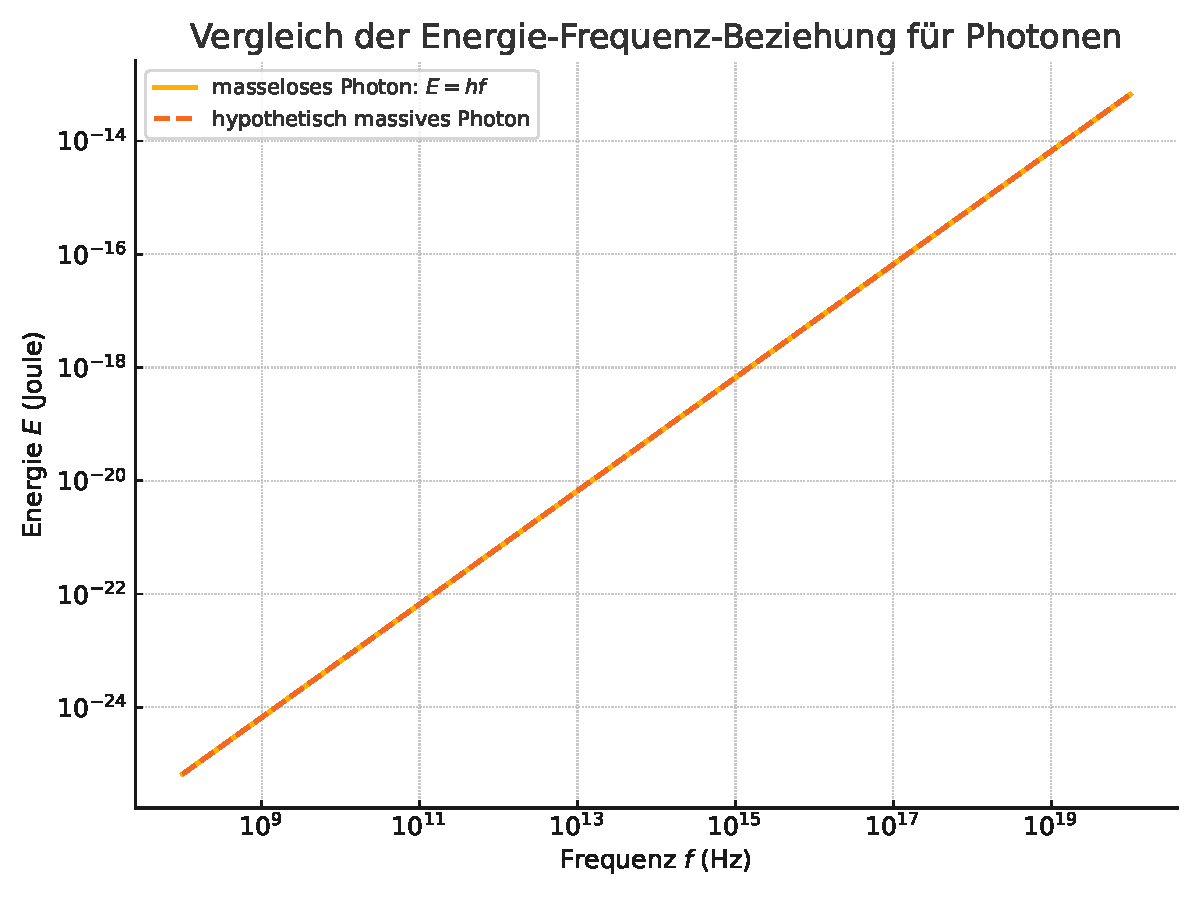
\includegraphics[width=0.85\textwidth]{bilder/photon_energie_vergleich_didaktisch.pdf}
	\caption{Didactic comparison of the energy–frequency relation \( E(f) \) for a massless photon (blue) and a hypothetical massive photon with exaggerated mass (red, dashed).}
	\label{fig:energie_f_masselos_massiv}
\end{figure}
\vspace{1em}
\begin{tcolorbox}[hinweisbox, title=Why No Difference Is Visible in the Plot]
	\label{box:Warum sieht man}
	The $E(f)$ relation is shown for massless and (exaggerated) massive photons. Because the experimental upper bound on the photon mass is so tiny ($m_\gamma < 10^{-54}$ kg), the two curves are practically indistinguishable even on log–log scales. \\[1ex]
	\textbf{This lack of deviation strongly supports the photon’s masslessness.}
\end{tcolorbox}
\vspace{1em}
\begin{tcolorbox}[hypobox, title={What if the Photon Had a Mass?}]
	\label{box:was wäre wenn}
	If the photon had even a tiny mass ($m_\gamma > 0$), then:
	\begin{itemize}
		\item It would travel more slowly than the speed of light ($v < c$),
		\item The energy–frequency relation would not be $E=hf$, but
		$$
		E = \sqrt{(hf)^2 + (m_\gamma c^2)^2}\,,
		$$
		\item The speed of light would not be universal – e.g., long-wavelength light would be slower than short-wavelength light,
		\item Coulomb’s law would be \emph{screened} – electric fields would have finite range.
	\end{itemize}
	Since none of this is observed, the photon is, with overwhelming evidence, truly massless.
\end{tcolorbox}
\vspace{1em}
\newpage
\noindent
\subsubsection{Why Would \( E = h f \) Fail for a Massive Photon?}

The formula $E = hf$ holds exactly only for massless particles. If the photon had mass, one would have
$$
E = \sqrt{(hf)^2 + (m_\gamma c^2)^2} \; > \; hf\,,
$$
so the energy would not depend on frequency alone – something that would be experimentally detectable.

\paragraph{Confirmed Experiments:}
\begin{itemize}
	\item Photoelectric effect
	\item Compton effect
	\item Spectral lines and laser spectroscopy
	\item Quantum optics and precision QED experiments
\end{itemize}
All confirm, to high precision, the relation $E = hf$. No systematic deviation has ever been found.
\vspace{1em}
\begin{tcolorbox}[physikbox, title=Conclusion: Why the Photon Is Massless]
	\label{box:Warum das Photon}
	\begin{itemize}
		\item The photon has no rest mass ($m_0 = 0$) but does have energy and momentum.
		\item It necessarily propagates at the speed of light: $v = c$.
		\item Only under this condition do $E = pc$ and $E = hf$ hold.
		\item If $m_\gamma > 0$, numerous observations and special relativity would be contradicted.
	\end{itemize}
\end{tcolorbox}
\vspace{1em}

\newpage
\noindent
\subsection{Spin and Polarization}\index{Spin}\index{Polarization}\index{Boson}\index{Helicity}

\subsubsection{Spin of the Photon}

In quantum mechanics, \textbf{spin} is a fundamental property of elementary particles – comparable to an intrinsic angular momentum. Unlike classical rotation, spin does not refer to literal spinning in space; it is a purely quantum property with discrete values.

\vspace{0.5em}
\textbf{Photons have spin 1} and thus belong to the class of \textit{bosons}. While half-integer spin particles (like electrons with spin $1/2$) are fermions and obey the Pauli principle, bosons can occupy the same quantum state – a principle with fundamental consequences for light, e.g., laser amplification.\index{Fermion}\index{Pauli principle}\index{Laser}
\vspace{1em}
\begin{tcolorbox}[physikbox, title=Properties of Photon Spin]
	\label{box:Eigenschaften des}
	\begin{itemize}
		\item Photons have \textbf{spin 1} but no rest mass.
		\item Only two measurable spin states exist: \textbf{helicity $+1$ and $-1$}.
		\item The \textbf{spin direction} is always along the photon’s direction of motion.
	\end{itemize}
\end{tcolorbox}
\vspace{1em}
The restriction to only two spin states is a direct consequence of the photon’s \textbf{masslessness}. In contrast to massive spin‑1 particles (e.g., the Z boson), there is no rest frame for the photon; thus the longitudinal ($0$) spin state is absent. Only the two transverse helicity modes $\pm 1$ remain.\index{Z boson}

(A formal derivation of the allowed photon helicities is given in Appendix~A, Sec.~\ref{anhangA:helizitaet}.)

\newpage
\noindent
\textbf{Helicity} is the projection of spin onto the direction of motion:
\begin{itemize}
	\item \textbf{Helicity $+1$:} right‑circularly polarized light.
	\item \textbf{Helicity $-1$:} left‑circularly polarized light.
\end{itemize}

\begin{figure}[H]
	\centering
	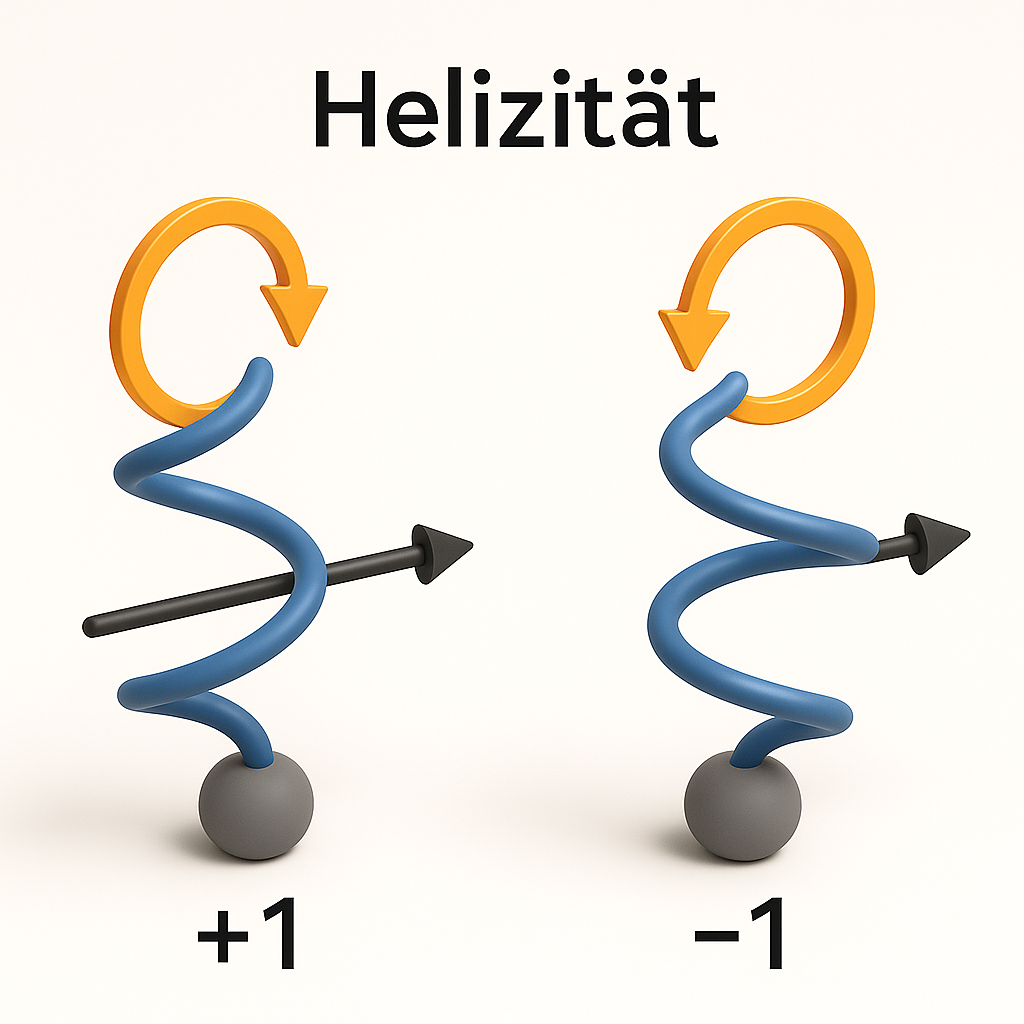
\includegraphics[width=0.65\textwidth]{bilder/Helizitaet.png}
	\caption{Visualization of photon helicity. Left: helicity $+1$ (right‑circular), right: helicity $-1$ (left‑circular). Orange arrows indicate spin (field rotation), black arrows indicate propagation direction.}
	\label{fig:helizitaet}
\end{figure}

\begin{tcolorbox}[physikbox, title=Comment on the Illustration]
	\label{box:Kommentar zur Darstellung}
	The spiral depicts how the electric field vector rotates for circular polarization. The photon travels straight along the propagation direction (momentum arrow). The spiral shows rotation of the field – not the photon’s path. This distinction is crucial for understanding helicity.
\end{tcolorbox}
\vspace{1em}
These two states underpin \textit{circular polarization}, discussed next.

\newpage
\noindent
For comparison:
\begin{itemize}
	\item An \textbf{electron} has spin $1/2$ with two states (up/down).
	\item A \textbf{Z boson} (massive, spin 1) exhibits three states: $-1$, $0$, $+1$.
	\item The \textbf{photon} (massless, spin 1) exhibits only $-1$ and $+1$ – the $0$ state is absent.
\end{itemize}
\vspace{1em}
\begin{tcolorbox}[physikbox, title=Didactic Rule of Thumb]
	\label{box:didaktischerMerksatz}
	Massless spin‑1 particles such as photons possess only two helicity states: \textbf{$\pm1$}. A longitudinal ($0$) state does not exist because no rest frame can be defined.
\end{tcolorbox}
\vspace{1em}

\subsubsection*{Conclusion}
\phantomsection
The photon’s spin fundamentally differs from that of massive particles. As a massless spin‑1 particle, the photon has only two helicity states: $+1$ and $-1$. A longitudinal helicity‑0 state is excluded because no rest frame exists.

\vspace{0.5em}
Spin can thus only be considered along the direction of motion – it manifests as helicity:
\begin{itemize}
	\item Helicity $+1$: spin aligned with motion (right‑circular)
	\item Helicity $-1$: spin opposite to motion (left‑circular)
\end{itemize}
A classical picture of literal rotation is inapplicable. Spin is an intrinsic quantum property that appears, for photons, as circular polarization.

\subsubsection{Polarization as a Macroscopic Manifestation of Spin}

Polarization is an observable phenomenon directly linked to the quantum spin of photons. While spin is an intrinsic property of each photon, polarization describes the collective state of a light field – i.e., many photons together.

\vspace{0.5em}
Classically, polarization is the orientation of the electric field vector of an electromagnetic wave. This vector oscillates transverse to the direction of propagation and can take different orientations and rotations:
\begin{itemize}
	\item \textbf{Linearly polarized light:} the electric field oscillates in a fixed direction (e.g., vertical or horizontal).
	\item \textbf{Circularly polarized light:} the field vector rotates at constant amplitude – clockwise (right‑circular) or counterclockwise (left‑circular).
	\item \textbf{Elliptically polarized light:} the most general case – the field vector traces an ellipse.
\end{itemize}
\index{Linearly polarized light}\index{Circularly polarized light}\index{Elliptically polarized light}

\vspace{0.5em}
In quantum optics, polarization corresponds to the collective helicity content of many photons.\index{Quantum optics} A fully right‑circularly polarized field consists of photons with helicity $+1$, a left‑circular field of photons with $-1$. Linear polarization arises from a quantum superposition of both helicity states:
$$
|\text{linear}\rangle = \frac{1}{\sqrt{2}} \bigl( |+1\rangle + |-1\rangle \bigr)
$$
(A more detailed treatment using Dirac notation and Jones vectors is given in Appendix~A, Sec.~\ref{anhangA:polarisation}.)
\vspace{1em}
\begin{tcolorbox}[physikbox, title=Superposition and Polarization]
	\label{box:Superposition}
	A linearly polarized photon is a quantum superposition of the two helicity states $|+1\rangle$ and $|-1\rangle$. This superposition leads to the fixed oscillation direction of the electric field.
\end{tcolorbox}

\vspace{0.5em}
Thus polarization is a directly observable consequence of photon spin. In many experiments – e.g., with polarizers, polarization cameras, or double-slit setups using polarized light – polarization appears as a macroscopic manifestation of quantum states.\index{Polarizer}
\vspace{1em}
\begin{tcolorbox}[physikbox, title=Superposition and Polarization]
	\label{box:Superposition und Polarisation}
	A linearly polarized photon is in a quantum superposition of the two helicity states $|+1\rangle$ (right‑circular) and $|-1\rangle$ (left‑circular):
	$$
	|\text{linear}\rangle = \frac{1}{\sqrt{2}} \left( |+1\rangle + |-1\rangle \right).
	$$
	This implies:
	\begin{itemize}
		\item The photon has no definite helicity.
		\item It is simultaneously in $|+1\rangle$ and $|-1\rangle$ with equal amplitude and fixed phase.
		\item The fixed oscillation direction (linear polarization) arises from this coherent superposition.
		\item Measuring helicity destroys the superposition: the photon is found with helicity $+1$ or $-1$ – never both at once.
	\end{itemize}
	Polarization is therefore more than a field direction – it is the expression of a quantum state that is fully captured only via superposition.
\end{tcolorbox}

\subsubsection{Measuring and Detecting Polarization}

Polarization is a macroscopic observable consequence of the photon’s quantum spin structure. Various optical methods are available – from simple polarizers to precise single‑photon detectors in quantum optics.

\vspace{0.5em}
\textbf{Linear polarization} can be tested classically with two polarizers: a linearly polarized beam passes a second polarizer (the “analyzer”). The transmitted intensity varies with the relative angle according to \textbf{Malus’s law}:\index{Malus’s law}
$$
I = I_0 \cos^2\theta
$$
where \( \theta \) is the angle between the incident polarization and the analyzer axis.

\vspace{0.5em}
\textbf{Circular polarization} is revealed by combining a linear polarizer with a quarter‑wave plate,\index{Quarter-wave plate} which converts circular to linear polarization for analysis.

\vspace{0.5em}
\textbf{Single‑photon experiments} in quantum optics directly probe quantized polarization:
\begin{itemize}
	\item A photon impinges on a polarizer and is either transmitted or absorbed.
	\item Repeated measurements on identically prepared photons yield polarization statistics.
	\item These experiments show: polarization is a single‑photon phenomenon, not merely a classical wave effect.
\end{itemize}

\vspace{0.5em}
\textbf{Technical applications} abound:
\begin{itemize}
	\item LCD displays, polarized sunglasses, remote sensing
	\item Communications using polarization multiplexing (e.g., in fiber optics)
	\item Quantum communication with polarized single photons (QKD)
\end{itemize}
\index{QKD (quantum key distribution)}\index{Polarization multiplexing}

\begin{tcolorbox}[physikbox, title=What Polarization Reveals About Photons]
	\label{box:Was uns die}
	Polarization is not only a property of electromagnetic waves but a directly measurable result of photon spin. Polarization measurements allow fundamental statements about the states of single light quanta – up to and including entanglement in quantum physics.
\end{tcolorbox}
\index{Entanglement}

\subsection{Conclusion }\index{Conclusion}

Chapter~III has shown how light can be understood, from the quantum‑mechanical viewpoint, not only as an electromagnetic wave but also as a particle – the photon. This understanding unites classical concepts such as frequency and polarization with quantized properties such as energy, momentum, and spin.

\vspace{0.5em}
Key insights:
\begin{itemize}
	\item A photon’s energy is directly proportional to its frequency: \( E = h\nu \).
	\item A photon’s momentum is determined by its wavelength: \( p = \tfrac{h}{\lambda} \).
	\item Photons have spin~1 but, due to masslessness, only the helicity states $+1$ and $-1$ occur.
	\item The polarization of macroscopic light fields is a collective phenomenon rooted in the quantum states of many photons.
\end{itemize}

\vspace{0.5em}
These quantized properties of the photon will play a central role in Chapter~IV, where we explore the wave nature of particles and the particle nature of waves in the form of wave–particle duality.

	\chapter{Experimental Confirmation of the Photon}
\setcounter{section}{4}
\setcounter{subsection}{0}
\setcounter{subsubsection}{1}
\setcounter{secnumdepth}{3}
\setlength{\parindent}{0pt}
% Box styles
\tcbset{physikbox/.style={colback=blue!5!white, colframe=blue!75!black, fonttitle=\bfseries}}
\tcbset{mathebox/.style={colback=green!5!white, colframe=green!50!black, fonttitle=\bfseries}}
\tcbset{didaktikbox/.style={colback=yellow!5!white, colframe=yellow!50!black, fonttitle=\bfseries}}
\tcbset{hypobox/.style={colback=orange!5!white, colframe=orange!75!black, fonttitle=\bfseries}}
\tcbset{hinweisbox/.style={colback=gray!10!white, colframe=black!40!black, fonttitle=\bfseries}}

\subsection{The Photoelectric Effect}\index{Photoelectric Effect}

\subsubsection{Introduction and Classical Expectation}\index{Classical Electrodynamics}\index{Wave Model}

The so-called photoelectric effect – the emission of electrons from a metal surface when irradiated with light – was already known in the 19th century. Heinrich Hertz\index{Hertz, Heinrich} discovered the phenomenon in 1887 by accident during his investigations of electromagnetic radiation. Philipp Lenard\index{Lenard, Philipp} later studied it systematically and found: electrons are released from the metal when exposed to certain kinds of light.

Classical electrodynamics explained this behavior using the wave model of light\index{Wave Model}. According to that model, the energy of light should be transferred continuously to the electron via the electric field strength. From this, three seemingly plausible expectations followed:

\begin{itemize}
	\item \textbf{Intensity decides:} The higher the light intensity, the more energetic the emitted electrons should be.
	\item \textbf{Delay:} With weak light, a measurable time should pass until an electron has absorbed enough energy to be emitted.
	\item \textbf{Any wavelength possible:} In principle, any wavelength of light – even long-wave red light – should trigger electron emission if it is only intense enough.
\end{itemize}

These expectations seemed logical within the classical theory. But reality drastically contradicted them – a turning point in the history of physics.

\vspace{1em}
\begin{tcolorbox}[physikbox, title=Philipp Lenard (1902)\textit{ \cite{lenard1902} }]
	\label{box:Philipp Lenhard}
	
	\small
	“It turned out that light seemed to act with greater energy on electrons the shorter its wavelength was – regardless of how bright it was.”
\end{tcolorbox}

\subsubsection{Experimental Observations}

The systematic investigation of the photoelectric effect by Philipp Lenard\index{Lenard, Philipp}, Robert Millikan\index{Millikan, Robert A.}, and others led to observations that could not be reconciled with the classical wave theory. The central findings were:

\begin{itemize}
	\item \textbf{Immediate emission:} Electrons are released without measurable delay – even at extremely low light intensities.
	\item \textbf{Frequency dependence:} There exists a \emph{threshold frequency} \( \nu_{\text{min}} \)\index{Threshold Frequency}, below which no electrons are emitted – regardless of intensity.
	\item \textbf{Energy independent of intensity:} The kinetic energy of the emitted electrons depends solely on the frequency of the light – not on its intensity.
	\item \textbf{Linear relationship:} The electron energy increases linearly with the light frequency:
	\[
	E_{\text{kin}} = h \nu - A
	\]
	\index{Einstein Equation (Photoelectric Effect)}\index{Work Function}
\end{itemize}
(A more detailed derivation of Einstein’s equation for the photoelectric effect can be found in Appendix~A, Section~\ref{anhangA:photoeffekt}.)

These results fundamentally contradicted the classical expectation of continuous energy absorption from the electromagnetic field.

\vspace{1em}
\begin{tcolorbox}[physikbox, title=Albert Einstein (1905)\textit{ \cite{einstein1905}}]
	\label{die Erzeuguung von Licht}
	\small
	“The generation of light does not occur uniformly across the wavefront, but only at specific places, at individual points.”
\end{tcolorbox}
\index{Einstein, Albert}

\vspace{1em}
\begin{tcolorbox}[physikbox, title=Robert A. Millikan (1916)\textit{ \cite{millikan1916}}]
	\label{box:Robert A, Millikan}
	\small
	“Although I confirmed Einstein’s equation through years of experiments, I long resisted the idea that light consists of particles.”
\end{tcolorbox}
\vspace{1em}
\index{Millikan, Robert A.}

\textbf{Conclusion:} The observations could only be explained by assuming that light consists of discrete quanta – \emph{photons}\index{Photon}\index{Light Quantum|see{Photon}} – transferring their energy to an electron in a single collision. The classical wave picture had to be abandoned or profoundly modified.

\subsubsection{Einstein’s Explanation (1905)}\index{Einstein, Albert}\index{Light Quantum|see{Photon}}\index{Photon}\index{Heuristic Viewpoint (Einstein 1905)}

In 1905 Albert Einstein published his groundbreaking paper entitled \textit{“On a Heuristic Point of View Concerning the Production and Transformation of Light”} \cite{einstein1905}. In it he fundamentally questioned the classical idea of light as a continuous wave.\index{Classical Electrodynamics}\index{Wave Model}

Einstein proposed that light consists of individual energy portions – so-called \textbf{light quanta}\index{Light Quantum|see{Photon}}. These quanta carry a definite amount of energy:

\[
E = h \nu
\]\index{Planck–Einstein Relation@$E=h\nu$}

(A formal representation of the Planck–Einstein relation can be found in Appendix~A, Section~\ref{anhangA:planckEinstein}.)

A photon with frequency \( \nu \) thus possesses a discrete energy proportional to frequency. This idea was revolutionary, as it assigned a \emph{particle character} to light – contrary to the well-established Maxwell theory.\index{Maxwell, James Clerk}\index{Maxwell Theory}

Einstein further postulated that such a light quantum could transfer its energy completely to an electron in a collision. 

Only if the energy of the photon is greater than the so-called \textbf{work function} \( A \), an electron is released from the metal:\index{Work Function}

\[
E_{\text{kin}} = h \nu - A
\]\index{Einstein Equation (Photoelectric Effect)}

This equation explains directly:
\begin{itemize}
	\item Why only light of sufficiently high frequency can release electrons,
	\item Why emission occurs immediately (a single photon suffices),
	\item Why the kinetic energy of electrons grows linearly with frequency.
\end{itemize}

Einstein’s explanation was radical – and at first highly controversial. Even Max Planck, the founder of quantum theory, considered the light quantum hypothesis too speculative.\index{Planck, Max}

\vspace{1em}
\begin{tcolorbox}[physikbox, title=Albert Einstein (1905)\textit{ \cite{einstein1905}}]
	\label{die Erscheinung der Wärm}
	\small
	“The phenomena of thermal radiation demand a viewpoint according to which light consists of discrete quanta of energy in the direction of propagation.”
\end{tcolorbox}
\index{Einstein, Albert}
\vspace{1em}
\textbf{Assessment:} Einstein turned Planck’s mathematical trick into physical reality. With this he laid the foundation for the modern concept of the photon and the quantized nature of the electromagnetic field.\index{Photon}\index{Quantized Electromagnetic Field}

\subsubsection{Millikan’s Measurements (1916)}\index{Millikan, Robert A.}

Although Einstein’s light quantum hypothesis provided a convincing explanation for the photoelectric effect, it was initially heavily disputed. Many physicists – including Max Planck – considered it unimaginable that light should consist of real particles.\index{Planck, Max} One of the most prominent skeptics was \textbf{Robert A. Millikan}.\index{Millikan, Robert A.}

In a series of experiments (1909–1916), Millikan developed a particularly precise setup to systematically test Einstein’s equation. Using a vacuum photo cell\index{Vacuum Photocell}, finely adjustable counter voltages\index{Counter Voltage}, and monochromatic light sources\index{Monochromatic Light}, he was able to directly measure the maximum kinetic energy of the electrons at different light frequencies.

\textbf{The result:} Despite all his doubts, Millikan found a crystal-clear confirmation of Einstein’s prediction:

\[
e U = h \nu - A
\]\index{Einstein Equation (Photoelectric Effect)}\index{Work Function}

(A detailed derivation of the stopping voltage equation and its experimental significance can be found in Appendix~A, Section~\ref{anhangA:stoppspannung}.)

Here \( U \) is the counter voltage required to fully suppress the electron current. The slope of the resulting straight line (electron energy vs. frequency) yielded with high accuracy Planck’s constant \( h \).\index{Planck’s Constant@$h$ (Planck’s Constant)}

\vspace{1em}
\begin{tcolorbox}[physikbox, title=Robert A. Millikan (1916)\textit{ \cite{millikan1916}}]
	\label{box:einsteins gleichung passt}
	\small
	“Einstein’s equation matches the data with astonishing accuracy – and yet I cannot bring myself to regard it as theoretically satisfying.”
\end{tcolorbox}
\index{Millikan, Robert A.}
\vspace{1em}

\textbf{Remarkable:} With utmost precision, Millikan disproved the classical theory – and confirmed Einstein’s light quantum – but was reluctant to accept the concept. Only years later did he recognize the quantized nature of light as physical reality.

\textbf{Significance:} Millikan’s measurements are considered one of the most important experimental proofs of the photon concept.\index{Photon} They strengthened the acceptance of Einstein’s theory – although it was only fully appreciated with the development of quantum mechanics.\index{Quantum Mechanics}

\subsubsection{Mathematical Description}\index{Einstein Equation (Photoelectric Effect)}\index{Work Function}

The central formula for describing the photoelectric effect is based on Einstein’s assumption that each photon possesses a discrete energy \( E = h\nu \).\index{Planck–Einstein Relation@$E=h\nu$} When such a photon hits an electron in the metal, its energy is transferred to the electron. The energy balance is:

\[
E_{\text{Photon}} = E_{\text{Work Function}} + E_{\text{kin}}
\quad\Rightarrow\quad h \nu = A + E_{\text{kin}}
\]\index{Einstein Equation (Photoelectric Effect)}


Where:

- \( h \) is Planck’s constant\index{Planck’s Constant@$h$ (Planck’s Constant)}  
- \( \nu \) is the frequency of the incident light\index{Frequency}  
- \( A \) is the material-dependent \textbf{work function}\index{Work Function}  
- \( E_{\text{kin}} \) is the kinetic energy of the electron\index{Kinetic Energy}

If a counter voltage \( U \) is applied to suppress the electron current, then the energy \( e U \) corresponds to the maximum kinetic energy of the electrons:\index{Counter Voltage}\index{Stopping Voltage@Stopping Voltage (Photoelectric Effect)}

\[
eU = h \nu - A
\]\index{Einstein Equation (Photoelectric Effect)}

This is the experimentally measurable form of Einstein’s equation.

\vspace{0.5em}
\begin{tcolorbox}[physikbox, title=What is the Work Function \( A \)?]
	\label{bos:was ist Austrittsarbeit}
	\small
	The work function \( A \) is the minimum energy required to release an electron from the metal. It depends on the material and typically lies between 2\,eV (e.g. cesium) and 5\,eV (e.g. platinum). Only if \( h \nu > A \), an electron is emitted.
\end{tcolorbox}
\vspace{1em}

\textbf{Graphical representation:}\index{Stopping Voltage@Stopping Voltage (Photoelectric Effect)}\index{Threshold Frequency}

The equation describes a \textit{linear dependence} of electron energy (or stopping voltage \( U \)) on frequency \( \nu \). The graph is a straight line:
\begin{figure}[H]
	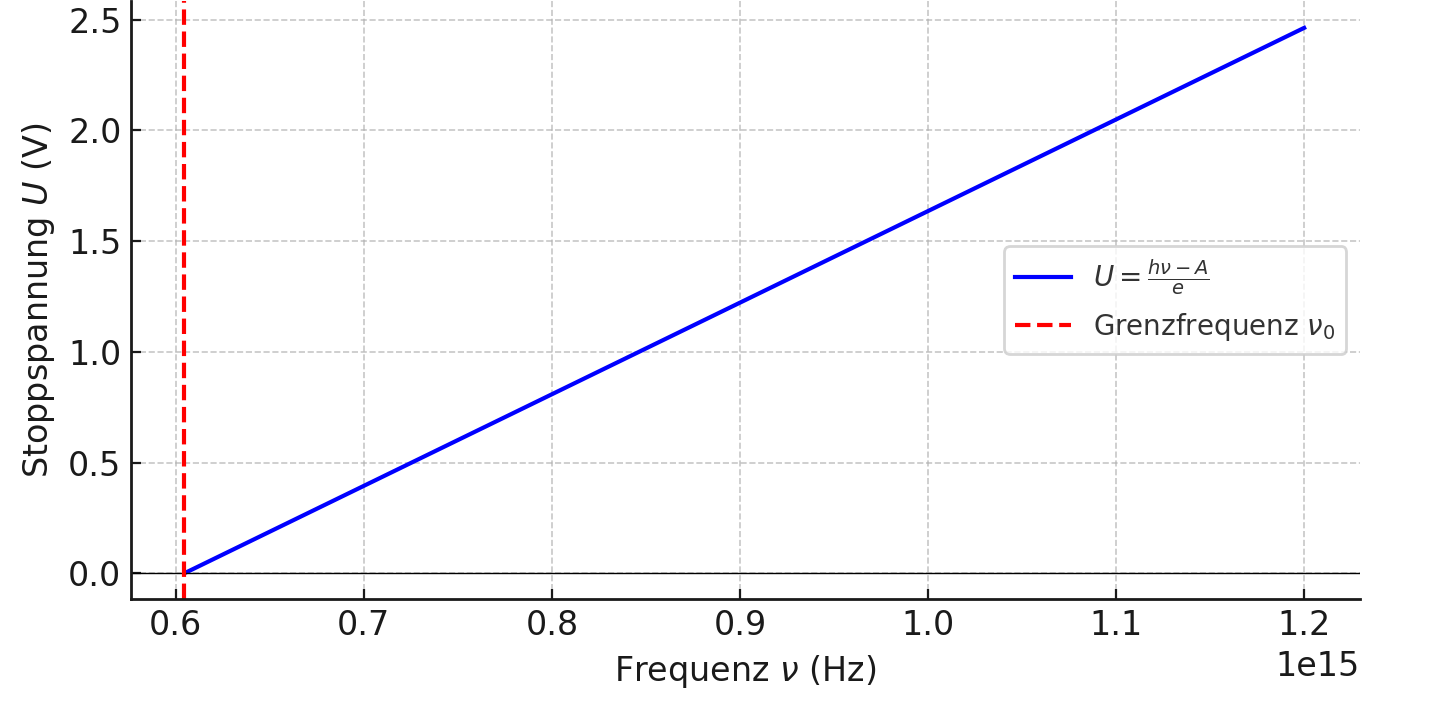
\includegraphics[width=0.65\textwidth]{bilder/photoeffekt.png}
	\caption{Linear dependence of electron energy on frequency.}
\end{figure}

\begin{itemize}
	\item The \textbf{slope} of the line corresponds to \( h/e \)
	\item The \textbf{x-intercept} \( \nu_0 \) is the threshold frequency: \( h \nu_0 = A \)\index{Threshold Frequency}
	\item For \( \nu < \nu_0 \) no emission occurs – regardless of intensity
\end{itemize}

This linear relationship was experimentally confirmed with high accuracy by Millikan.\index{Millikan, Robert A.}

\textbf{Consequence:}

\begin{quote}
	The energy of a photon depends solely on its frequency – not on light intensity.
\end{quote}
\index{Frequency}\index{Intensity}

\subsubsection{Comparison: Wave Model vs. Photon Model}\index{Wave Model}\index{Photon Model}\index{Wave–Particle Duality@Wave–Particle Duality (Contrast)}

Explaining the photoelectric effect marked a profound paradigm shift in physics: from the classical wave picture of light to a quantized particle model.\index{Paradigm Shift} To illustrate the significance of this change, it is useful to directly compare both models.

\vspace{1em}
\begin{table}[H]
	\centering
	\begin{tabular}{|p{4.75cm}|p{4.75cm}|}
		\hline
		\textbf{Classical Wave Model} & \textbf{Photon Model (Einstein)} \\
		\hline
		Light is a continuous wave in the electromagnetic field & Light consists of individual quanta (photons) with energy \( E = h\nu \) \\
		\hline
		Energy is transferred continuously via field strength & Energy is transferred abruptly in discrete portions \\
		\hline
		Intensity determines the energy transfer & Intensity only determines the \emph{number} of photons, not their energy \\
		\hline
		Any frequency can release electrons if intensity is high enough & Only photons with \( h\nu > A \) release electrons \\
		\hline
		Energy is accumulated slowly; time delay possible & Immediate emission when a photon strikes \\
		\hline
	\end{tabular}
	\caption{Comparison between the classical wave model and Einstein’s photon model for the photoelectric effect}
	\label{tab:vergleich_photoeffekt}
\end{table}

\vspace{1em}

\begin{tcolorbox}[didaktikbox, title=Didactic Clarification]
	\label{box:didaktischeKlarstellung}
	\small
	In the wave model, light intensity determines the strength of energy transfer – in the photon model, however, it only determines the number of incident quanta.\\
	The energy of an individual photon depends exclusively on frequency.
\end{tcolorbox}
\vspace{1em}
\index{Intensity}\index{Frequency}\index{Photon}

\textbf{Typical Misunderstanding:}  
“Bright light must release more energetic electrons.”  
$\rightarrow$ \emph{False}, because with light below the threshold frequency nothing happens – regardless of brightness.\index{Threshold Frequency}

\textbf{Assessment:}  
The photoelectric effect was the first direct proof that electromagnetic radiation has not only wave character, but also particle properties. This duality was later generalized in the concept of wave–particle duality.\index{Wave–Particle Duality}

\subsubsection{Significance for Physics}\index{Photoelectric Effect!Significance}\index{Photon}\index{Quantized Nature of Light}\index{Einstein, Albert}\index{Classical Electrodynamics}

The photoelectric effect was the first phenomenon that could only be explained by assuming a quantized nature of light. Einstein’s light quantum hypothesis of 1905 contradicted classical electrodynamics and was initially dismissed as speculative. But Millikan’s precise confirmation in 1916 forced the scientific community to fundamentally rethink the concept of light.\index{Millikan, Robert A.}

\textbf{Physical Consequences:}
\begin{itemize}
	\item Energy transfer of light does not occur continuously, but in discrete quanta – the photons.\index{Photon}
	\item The energy of a photon is proportional to frequency: \( E = h\nu \).\index{Planck–Einstein Relation@$E=h\nu$}\index{Frequency}
	\item The photoelectric effect provided the first direct experimental proof of this quantization.\index{Photoelectric Effect!Proof}
\end{itemize}

Einstein himself received the Nobel Prize in 1921 – explicitly not for relativity, but:\index{Nobel Prize!Einstein 1921}\index{Theory of Relativity}
\begin{quote}
	“for his services to theoretical physics, and especially for his discovery of the law of the photoelectric effect.”
\end{quote}

Millikan was also awarded the Nobel Prize in 1923 – for his determination of the elementary charge and his work on the photoelectric effect.\index{Nobel Prize!Millikan 1923}\index{Elementary Charge}

\vspace{1em}
\begin{tcolorbox}[hinweisbox, title=Conclusion]
	\label{box:fazit der photo}
	\small
	The photoelectric effect marks the beginning of the photon concept – and thus the dawn of quantum physics.\\
	It shows: light not only has wave properties, but under certain conditions behaves like a particle.
\end{tcolorbox}
\index{Quantum Physics}
\vspace{1em}

\textbf{Outlook:}  
In the next section we will consider another key experiment: \textbf{Compton scattering}. It demonstrates not only the energy transfer, but also the \emph{momentum transfer} of photons – a decisive proof of the particle character of light.\index{Compton Scattering}\index{Momentum Transfer}

\subsection{Compton Scattering}\index{Compton Scattering}\index{Compton, Arthur H.}\index{X-rays}

\subsubsection{The Compton Experiment (1923)}\index{Compton, Arthur H.!Experiment (1923)}

In 1923 the American physicist \textbf{Arthur H. Compton} published the results of a scattering experiment with X-rays that would revolutionize physics. He directed high-energy photons onto nearly free electrons – for example in graphite – and analyzed the scattered radiation as a function of angle.\index{Electron}\index{Graphite}

The central observation was striking: the scattered light had a longer wavelength (lower energy) than the incident light, and the wavelength shift depended systematically on the scattering angle.\index{Wavelength Shift}\index{Scattering Angle}

This change could not be explained by classical scattering (such as Thomson scattering) or interference. Compton interpreted the result as an \textbf{elastic collision} between a photon and an electron – fully in line with a particle model of light. Thus the photon was not only a carrier of energy, but also of momentum.\index{Thomson Scattering}\index{Elastic Collision}\index{Photon Momentum}

\textbf{Physical principle:}
\begin{itemize}
	\item A photon with wavelength \( \lambda \) strikes a stationary electron.
	\item During the collision the photon is deflected (scattering angle \( \theta \)) and transfers momentum and energy to the electron.
	\item The scattered photon has a new wavelength \( \lambda' > \lambda \).
\end{itemize}

\textbf{Key equation:}
\[
\Delta \lambda = \lambda' - \lambda = \frac{h}{m_e c}(1 - \cos \theta)
\]\index{Compton Formula}\index{Compton Wavelength}\index{Electron!Mass $m_e$}

\vspace{1em}
\begin{figure}[H]
	\begin{center}
		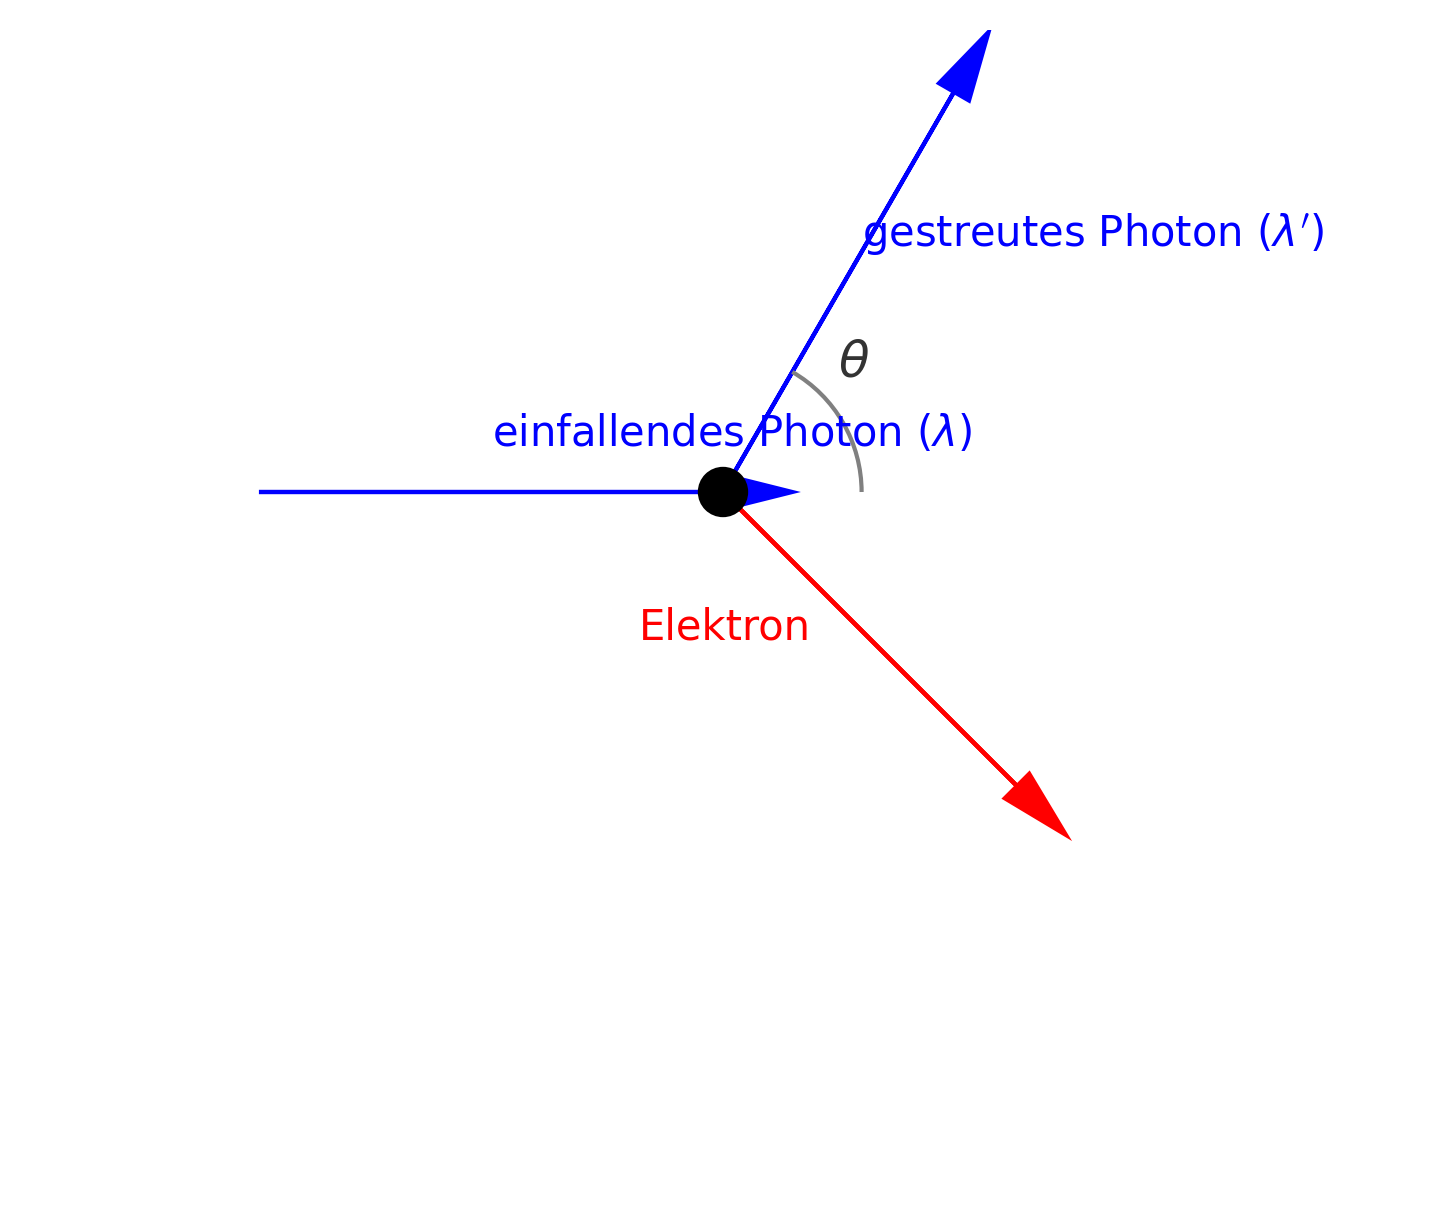
\includegraphics[width=0.6\textwidth]{bilder/compton-schema.png}
	\end{center}
	\caption{Schematic representation of Compton scattering: a photon transfers momentum to an electron.}
\end{figure}

\textbf{Significance:}  
Compton scattering was the first experimental proof that photons possess momentum – a decisive step toward accepting the photon as a real particle. Arthur Compton received the Nobel Prize in Physics in 1927 for this.\index{Photon Momentum}\index{Nobel Prize!Compton 1927}
\newpage
\noindent
\subsubsection{Compact Derivation of the Compton Formula}\index{Compton Formula!Derivation}\index{Energy Conservation}\index{Momentum Conservation}

The central observation in the Compton effect is: the scattered photon has a longer wavelength than the incident photon. This shift can only be explained if the photon is assigned not only energy \( E = h\nu \), but also momentum \( p = h/\lambda \).\index{Planck–Einstein Relation@$E=h\nu$}\index{Photon Momentum}

\textbf{Basic idea of the derivation:}  
A photon strikes a stationary electron. During the collision, energy and momentum are transferred to the electron. The situation resembles an elastic collision of two particles – with the difference that one of them is massless.\index{Elastic Collision}\index{Massless Particles}


\textbf{Core assumptions:}
\begin{itemize}
	\item \textbf{Energy conservation:} The sum of photon energy and electron rest energy is conserved.
	\item \textbf{Momentum conservation:} The momentum vectors before and after the collision must balance – in both x- and y-directions.
	\item \textbf{Photon momentum:} For the photon \( p = \frac{h}{\lambda} \), for the electron the relativistic energy–momentum relation applies.\index{Relativistic Energy–Momentum Relation}
\end{itemize}

Applying these conservation laws and simplifying yields the \textbf{Compton formula}:

\vspace{1em}
\begin{tcolorbox}[mathebox, title=Compton Formula]
	\label{box:comptonFormel}
	\small
	\[
	\Delta \lambda = \lambda' - \lambda = \frac{h}{m_e c}(1 - \cos \theta)
	\]
\end{tcolorbox}
\vspace{1em}
(A more detailed derivation of the Compton formula can be found in Appendix~A, Section~\ref{anhangA:comptonHerleitung}.) 

\textbf{Physical interpretation:}
\begin{itemize}
	\item The wavelength of the scattered photon increases with the scattering angle \( \theta \).\index{Scattering Angle}
	\item The factor \( \frac{h}{m_e c} \approx 2.43 \cdot 10^{-12}\,\mathrm{m} \) is known as the \emph{Compton wavelength} of the electron.\index{Compton Wavelength}
	\item The effect shows that the photon transfers \emph{momentum} – a clear proof of its particle character.\index{Photon Momentum}
\end{itemize}
\subsection{Double-Slit Experiment with Single Photons}\index{Double-Slit Experiment}\index{Single Photon}\index{Interference}\index{Wave–Particle Duality}

A central argument for the wave nature of light since the 19th century was the observation of interference patterns – in particular in the famous double-slit experiment. But modern experiments show: even single photons, sent one after another through the setup, produce an interference pattern on the screen. This is only explainable if the photon also possesses wave character.\index{Interference Pattern}


\textbf{Experimental setup:}
\begin{itemize}
	\item A weak light source emits single photons – so weak that never more than one is in the setup at the same time.\index{Single-Photon Source}
	\item The photons pass through two closely spaced slits (double slit).\index{Double Slit}
	\item Behind them is a light-sensitive screen or detector.\index{Detector}
\end{itemize}

\textbf{Observation:}
\begin{itemize}
	\item Each individual photon is registered as a point – like a particle.\index{Particle Aspect of Light}
	\item Over time, however, an interference pattern emerges – like a wave.\index{Wave Aspect of Light}
\end{itemize}

\vspace{1em}
\begin{figure}[H]
	\begin{center}
		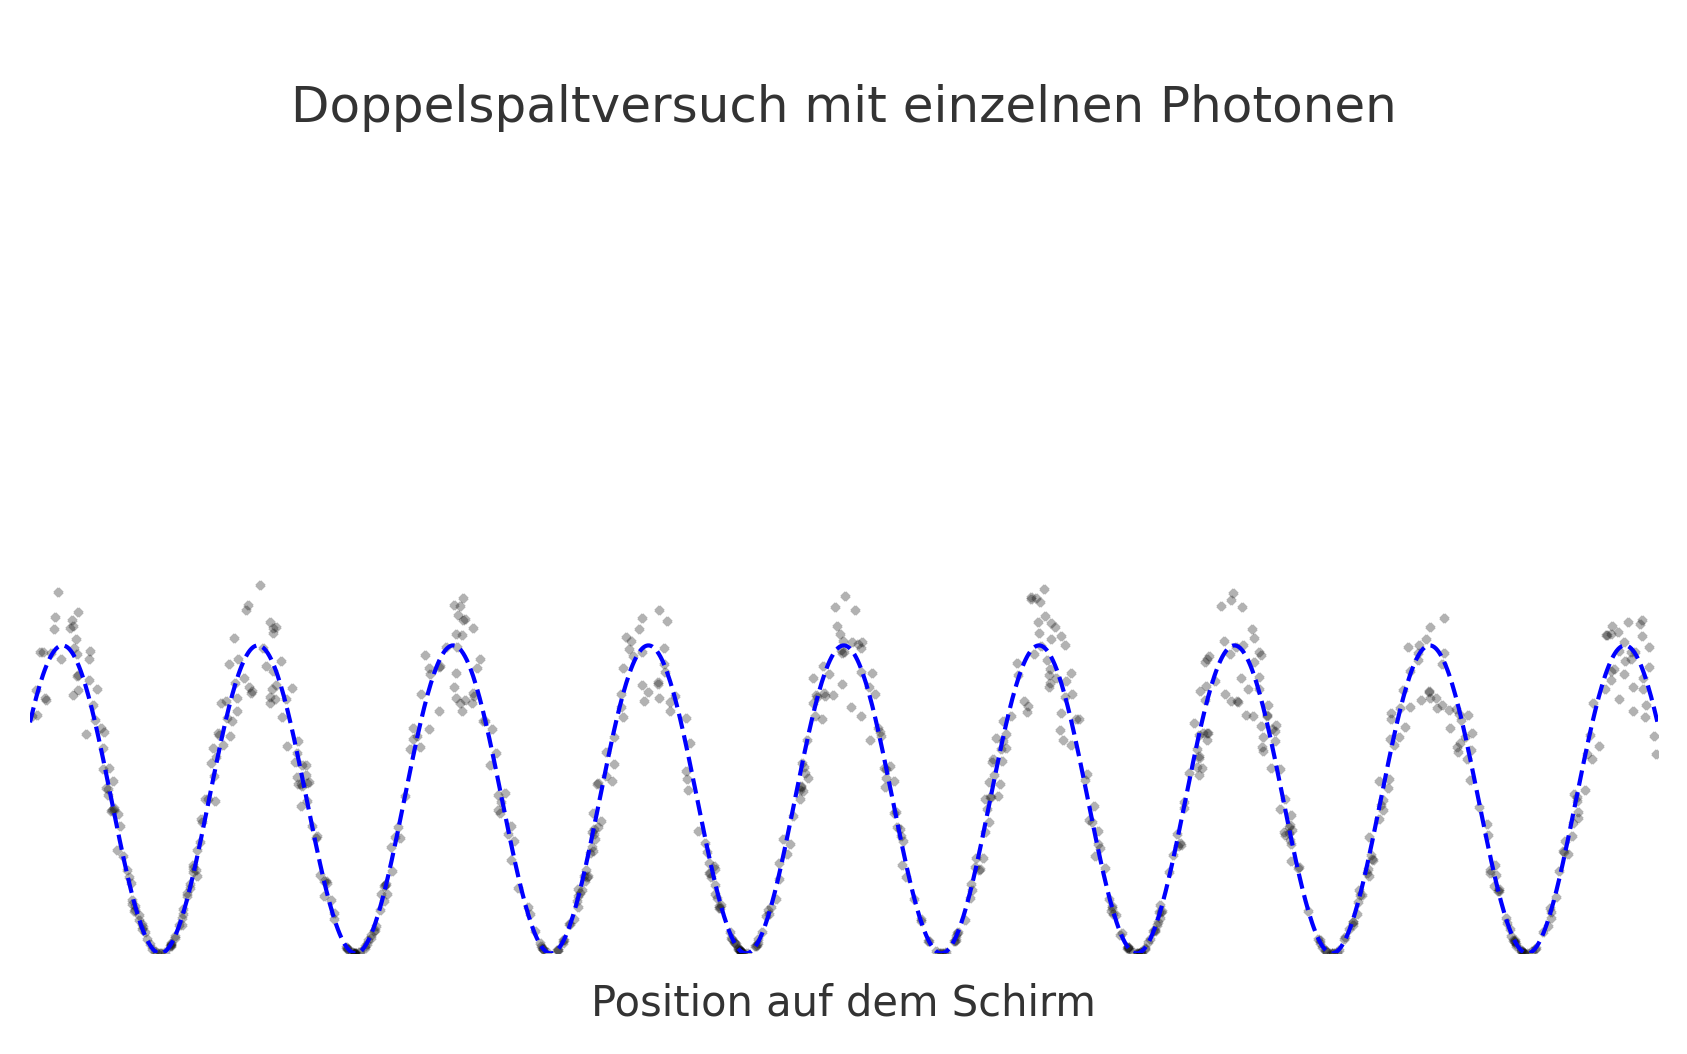
\includegraphics[width=0.65\textwidth]{bilder/doppelspalt-photonen.png}
	\end{center}
	\caption{Double-slit experiment with single photons: particle detections with a wave pattern.}
\end{figure}
\newpage
\noindent
\begin{tcolorbox}[physikbox, title=What the Photon Graphic is Meant to Show]
	\label{box:was die photonengrafik}
	\small
	\begin{itemize}
		\item The dots represent individual photon detections – the particle aspect of light.
		\item Over time a pattern emerges that is typical of wave interference – as with water waves.
		\item The dashed line shows only the statistical frequency of detection locations – it is not a light ray and not a real wave.
	\end{itemize}
\end{tcolorbox}
\vspace{1em}
(A mathematical formalization of the double-slit experiment with single photons and the superposition representation can be found in Appendix~A, Section~\ref{anhangA:doppelspalt}.) 

\textbf{Interpretation:}  
The photon apparently interferes with itself – it “passes through both slits simultaneously.” Only upon detection on the screen does the state collapse into a single event. This behavior can only be understood within quantum mechanics: the photon is neither a classical wave nor a classical particle – it exhibits both, depending on the experiment.\index{Self-Interference}\index{Quantum Mechanics}\index{Wavefunction Collapse}

\vspace{1em}
\begin{tcolorbox}[hypobox, title=Key Idea]
	\label{box:schlüsselidee}
	\small
	The double-slit experiment with single photons shows: the quantum nature of light encompasses both wave and particle properties. The interference pattern emerges even though never two photons are in the system at the same time.
\end{tcolorbox}
\vspace{1em}
\begin{tcolorbox}[didaktikbox, title=Wave as well as Particle Properties]
	\label{box:wellen}
	\small
	The interference pattern disappears immediately if one tries to determine the photon’s path through one of the slits. The possibility of interference is tied to the \emph{unknowability of the path} – a basic principle of quantum physics.
\end{tcolorbox}
\index{Which-Path Information}

\subsubsection*{Summary}\index{Double-Slit Experiment!Summary}\index{Superposition}

\phantomsection
\begin{tcolorbox}[didaktikbox, title=Conclusion: An Apparently Paradoxical Behavior]
	\label{box:Fazit ein scheinbarer}
	\small
	Even when photons are sent one by one – successively – through the double slit, an interference pattern emerges over time.
	
	This raises a profound question: How does a single photon “know” that it is part of a pattern?
	
	In classical terms there would have to be some kind of communication between photons – but that is not the case. Each photon seems to interfere with itself. Quantum mechanics explains this by the \textbf{superposition of all possible paths}: the photon has not gone through one or the other slit – but through both, as long as the path is not measured.
	
	This notion contradicts our everyday experience – but is experimentally beyond doubt. The double-slit experiment is therefore a key result of quantum physics.
	
	The double-slit experiment with single photons challenges our classical thinking:  
	How can a single photon contribute to building an interference pattern, although no second photon is present in the setup at the same time?
	
	Apparently each photon interferes with itself. In the language of quantum mechanics this means: as long as no measuring device determines the path, all possible paths are superposed – including “through both slits at once.”
	
	This superposition collapses only upon detection into a single point. The interference pattern arises not from interaction between photons, but from the \emph{statistics of many single measurements} – and from the quantum-mechanical structure of state space.
	
	What looks like “communication” is in fact an expression of the nonclassical nature of the quantum world.
\end{tcolorbox}

\subsection{Antibunching: The Proof of Single Photons}\index{Antibunching}\index{Single Photon}\index{Single-Photon Source}\index{Beam Splitter}\index{Detector}

A particularly convincing experimental proof for the existence of single photons is provided by the phenomenon of \textbf{antibunching}. Here a light source is used that emits only one photon at a time – for example, a fluorescing atom or a quantum dot.\index{Quantum Dot}\index{Fluorescence}

In a setup with a beam splitter and two detectors, it turns out: it \emph{never happens} that both detectors register a signal at the same time. This means: there is no such thing as “half a photon” – but always exactly one, which arrives either here or there.\\

\textbf{Why does this contradict the classical wave picture?} \\
In classical theory, light is a continuous electromagnetic wave. When such a wave strikes a beam splitter, it is \emph{divided}: one part goes left, the other right. Thus – at least with strong intensity – both detectors should sometimes register a signal simultaneously.\index{Classical Electrodynamics}\index{Wave Model}

In contrast, antibunching shows: \emph{never} are both detectors triggered at once. This means that the light does not arrive split, but in \textbf{indivisible energy packets} – single photons. This directly contradicts the classical wave picture.\index{Photon!Indivisibility}

\vspace{1em}
\begin{tcolorbox}[physikbox, title=What Antibunching Shows]
	\label{box:wasAntibunching}
	\small
	Light cannot be split into two directions simultaneously if it consists of single photons.\\
	This contradicts every classical wave picture – but precisely matches the behavior of indivisible light quanta.
\end{tcolorbox}
\vspace{1em}
(A mathematical description of the second-order correlation function \( g^{(2)}(0) \) can be found in Appendix~A, Section~\ref{anhangA:antibunching}.) 

\subsection{Hong–Ou–Mandel Effect: Interference of Two Photons}\index{Hong–Ou–Mandel Effect}\index{Photon Indistinguishability}\index{Probability Amplitude}\index{Beam Splitter}

Another striking experiment is the \textbf{Hong–Ou–Mandel (HOM) effect}. Two identical photons are sent from opposite directions onto a half-transparent mirror (beam splitter).

\begin{figure}[H]
	\begin{center}
		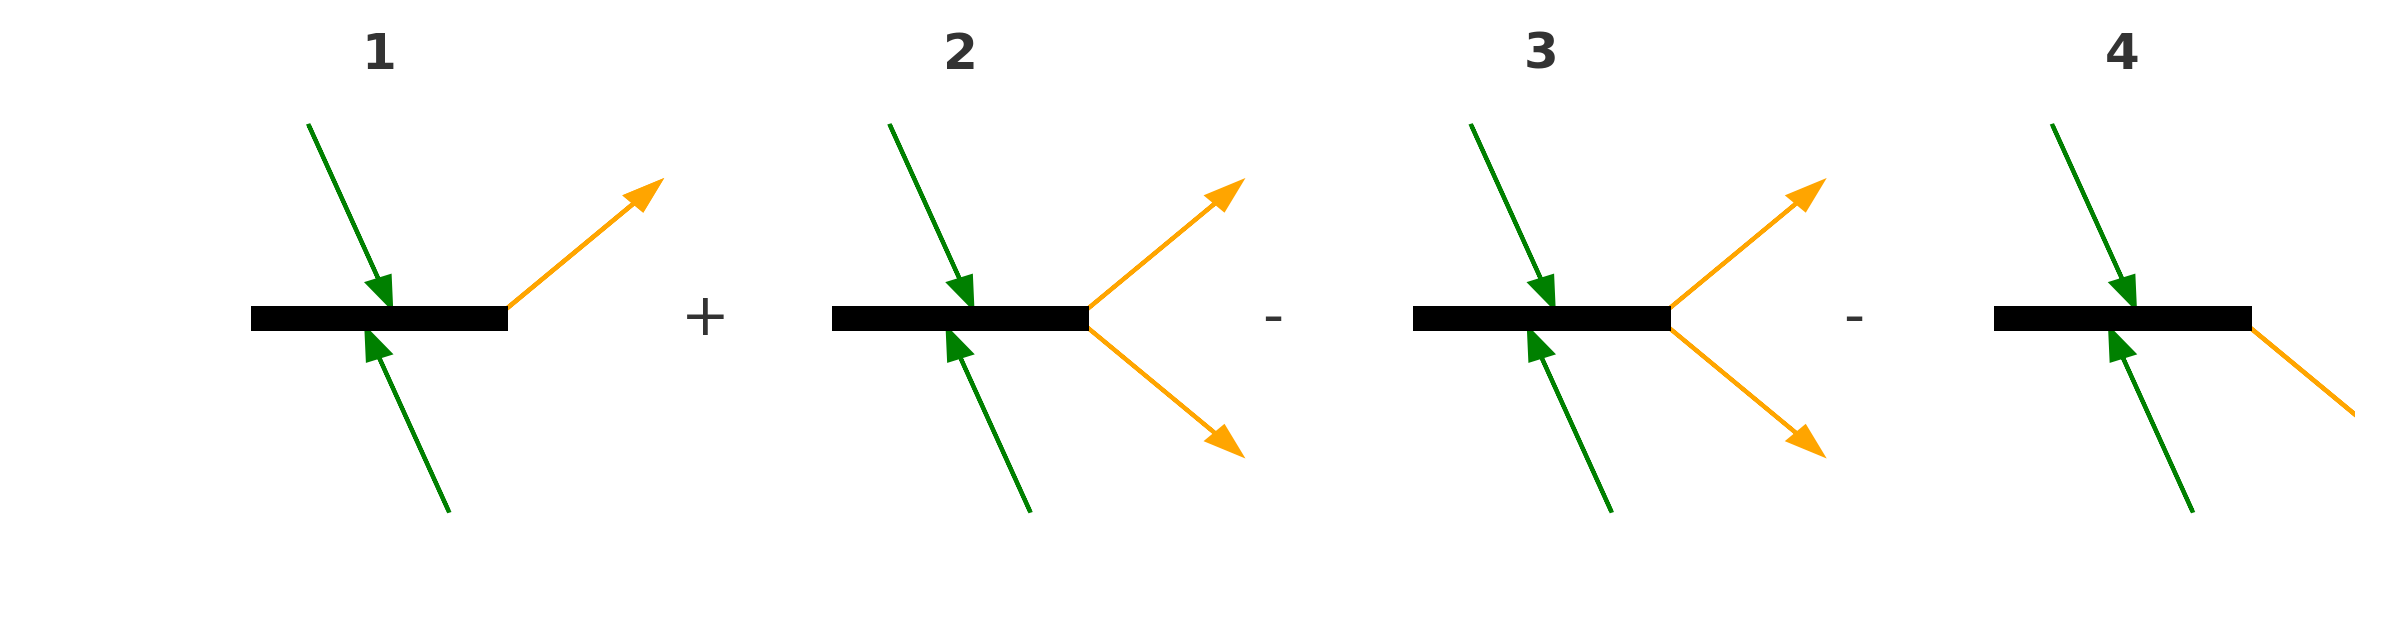
\includegraphics[width=0.95\textwidth]{bilder/hom_interferenzpfade_korrigiert.png}
	\end{center}
	\caption{Four possible paths of two photons at a beam splitter.\\
		The middle cases would lead to coincidence – but cancel due to interference.}
\end{figure}

\begin{tcolorbox}[hinweisbox, title=What This Diagram Shows]
	\label{box:was diese Darstellun}
	\small
	The diagram shows the four possible paths two identical photons can take when hitting a beam splitter.\\
	In cases 1 and 4 both photons exit together through the same output – exactly as observed experimentally.
	
	Paths 2 and 3 would lead to the photons arriving at different detectors (coincidence). But these cases cancel out due to destructive interference – because of the indistinguishability of the photons and the quantum-mechanical superposition of their amplitudes.
	
	The result: with perfect overlap both detectors are never triggered simultaneously – a clear sign of the quantum nature of light.
\end{tcolorbox}

According to classical expectation, each photon should be reflected or transmitted with 50% probability.\index{Reflection}\index{Transmission} But in quantum reality something different happens: both photons always leave through the same output – never opposite ones.

This phenomenon arises from the interference of the \emph{probability amplitudes} of the two processes. It shows: photons are indistinguishable and can interfere at the quantum level – not as fields, but as particles with wave nature.\index{Interference}\index{Photon Indistinguishability}

\vspace{1em}
\begin{tcolorbox}[physikbox, title=What the HOM Effect Shows]
	\label{box:HOM-Effekt}
	\small
	Two photons can “prevent” themselves from taking different paths – through the interference of their quantum states.\\
	This can only be explained if photons are considered indistinguishable quantum particles.
\end{tcolorbox}
\newpage
\noindent
\subsection{Conclusion}\index{Photoelectric Effect}\index{Compton Scattering}\index{Double-Slit Experiment}\index{Antibunching}\index{Hong–Ou–Mandel Effect}\index{Wave–Particle Duality}

\begin{tcolorbox}[hinweisbox, title=What the Experiments Show About Light]
	\label{box:was die Experimente}
	\small
	The four experiments discussed in this chapter – the photoelectric effect, Compton scattering, the double slit with single photons, and modern quantum experiments such as antibunching and the Hong–Ou–Mandel effect – demonstrate impressively that light cannot be explained by classical models alone.
	
	\begin{itemize}
		\item The \textbf{photoelectric effect} shows: light transfers \emph{energy} in discrete portions (photons).
		\item \textbf{Compton scattering} shows: photons also carry \emph{momentum} – like particles.
		\item The \textbf{double-slit experiment} shows: photons display \emph{wave patterns} in their distribution – even when occurring one at a time.
		\item \textbf{Antibunching} and the \textbf{Hong–Ou–Mandel effect} show: photons are \emph{indivisible}, \emph{non-classically indistinguishable}, and subject to the rules of quantum mechanics.
	\end{itemize}
	
	(A more detailed derivation of quantum interference at the beam splitter in the HOM effect can be found in Appendix~A, Section~\ref{anhangA:HOM}.) 
	
	Together these experiments prove: light is not an either–or of wave and particle – it is both at once, depending on the experiment. The photon concept is therefore not just a calculational tool – but physically real.
\end{tcolorbox}

	\chapter{The Photon in Quantum Electrodynamics (QED)}\index{Photon}\index{Quantum Electrodynamics (QED)}
\setcounter{section}{5}
\setcounter{subsection}{0}
\setcounter{subsubsection}{1}
\setcounter{secnumdepth}{3}
\setlength{\parindent}{0pt}
% Box styles
\tcbset{physikbox/.style={colback=blue!5!white, colframe=blue!75!black, fonttitle=\bfseries}}
\tcbset{mathebox/.style={colback=green!5!white, colframe=green!50!black, fonttitle=\bfseries}}
\tcbset{didaktikbox/.style={colback=yellow!5!white, colframe=yellow!50!black, fonttitle=\bfseries}}
\tcbset{hypobox/.style={colback=orange!5!white, colframe=orange!75!black, fonttitle=\bfseries}}
\tcbset{hinweisbox/.style={colback=gray!10!white, colframe=black!40!black, fonttitle=\bfseries}}
\tcbset{warnbox/.style={colback=red!10!white, colframe=red!40!black, fonttitle=\bfseries}}

\subsection{From the Photon to Quantum Electrodynamics}\index{Quantum Electrodynamics (QED)!Introduction}\index{Photoelectric Effect}\index{Compton Scattering}\index{Einstein, Albert}\index{Maxwell, James Clerk}\index{Exchange particle}
% Historical and theoretical transition: from classical electrodynamics via quantum optics to QED

The history of the photon begins with a paradox: Light, which since the 19th century was understood as an electromagnetic wave, showed behavior in certain experiments that could only be explained with a particle picture—particularly in the photoelectric effect and in Compton scattering.\index{Wave model}\index{Particle model}
These experiments led Einstein in 1905 to introduce the concept of the \emph{light quantum}.\index{Light quantum}
Although the photon model proved successful experimentally, it remained controversial for decades.\index{Photon model}

A complete theoretical understanding of light–matter interaction was achieved only with the development of \textbf{Quantum Electrodynamics} (QED).\index{Light–matter interaction}\index{Relativity!Special}\index{Quantum mechanics}
It unites Maxwell’s classical field theory with the principles of quantum mechanics and special relativity.
In QED, the photon is the exchange particle of the electromagnetic interaction—a massless, spin-1 gauge boson that can appear not only in real but also in virtual states.\index{Spin}\index{Masslessness}\index{Virtual photon}
(A compact introduction to the QED field formalism and the potential \(A^\mu\) can be found in Appendix~A, Section~\ref{anhangA:feldformalismus}.)
\newpage
\noindent
\vspace{1em}
\begin{tcolorbox}[physikbox, title=What is Quantum Electrodynamics?]
	\label{box:was ist quantenelektro}
	\small
	Quantum Electrodynamics describes how charged particles (e.g., electrons) exchange photons and thereby interact electromagnetically.\\
	The theory is based on quantized fields, Feynman diagrams, and a local gauge principle. It is the most precise physical theory ever tested experimentally.
\end{tcolorbox}
\vspace{1em}

The transition from classical to quantum field–theoretic understanding was anything but straightforward. At first, photons were treated as discrete packets of classical wave energy—a compromise between particle and wave pictures.\index{Quantum field theory}\index{Wave energy}
Only in the 1940s, through the work of Dirac, Feynman, Schwinger, and Tomonaga, did a consistent theory emerge that mathematically describes the photon as the quantum of the electromagnetic field.\index{Dirac, Paul A. M.}\index{Feynman, Richard P.}\index{Schwinger, Julian}\index{Tomonaga, Sin-Itiro}\index{Quantized field}

\textbf{What QED changes:}
\begin{itemize}
	\item Photons are no longer seen as light rays but as excitations of a quantized field.\index{Excitation (field)}\index{Light ray}
	\item Interaction occurs not continuously but in discrete processes (vertices).\index{Interaction!Vertex}
	\item Virtual photons—not directly observable but mathematically necessary—play a central role.\index{Virtual photon}
\end{itemize}
(For the transition from the classical field to quantization and to Feynman diagrams, see Appendix~A, Section~\ref{anhangA:feld_zu_qed}.)

This chapter introduces the properties of the photon within QED, beginning with its vector character, followed by its role as an exchange particle in Feynman diagrams, and ending with experimental confirmations of utmost precision.\index{Feynman diagram}

\subsection{The Vector Character of the Photon in QED}\index{Photon!Vector character}\index{Polarization!Transverse}\index{Spin}

The transverse polarization of the photon and its property as a spin-1 particle were already described in Section~3.6.\index{Helicity}
In Quantum Electrodynamics, however, this structure arises not only from experimental observation or classical equations, but from the underlying \emph{field formalism} and the \emph{gauge symmetry} of the theory.\index{Field formalism}\index{Gauge symmetry}
(A formal derivation of photon helicity is given in Appendix~A, Section~\ref{anhangA:helizitaet}; for polarization in Jones/Dirac notation, see \ref{anhangA:polarisation}.)

\vspace{1em}
\begin{tcolorbox}[physikbox, title=What is the Field Formalism?]
	\label{box:was ist Feldformalismus}
	\small
	In QED, photons are not “particles with trajectories,” but quantized excitations of a field: the electromagnetic potential \( A^\mu(x) \). Just as a water wave is a local displacement of the water surface, a photon is a discrete oscillation of the field—described simultaneously by quantum mechanics and relativity.
\end{tcolorbox}
\vspace{1em}
\index{Vector potential $A^\mu$}
(A short derivation of the Lorentz-covariant form of the four-potential \(A^\mu\) is given in Appendix~A, Section~\ref{anhangA:viererpotential}.)

The central mathematical starting point is the so-called \emph{Lagrangian density} \( \mathcal{L} \), from which the equations of motion of the field are derived.\index{Lagrangian density}\index{Equations of motion}
For the electromagnetic field it reads:

\[
\mathcal{L}_{\text{EM}} = -\frac{1}{4} F_{\mu\nu} F^{\mu\nu}
\quad \text{with} \quad F_{\mu\nu} = \partial_\mu A_\nu - \partial_\nu A_\mu
\]\index{Field strength tensor $F_{\mu\nu}$}
(Derivations of the field strength tensor and EM Lagrangian density: Appendix~A, Sections~\ref{anhangA:feldstaerketensor} and \ref{anhangA:lagrange_em}; for the energy–momentum relation see \ref{anhangA:energie_impuls}.)

This Lagrangian density leads—via the principle of least action—to Maxwell’s equations in their relativistic form.\index{Principle of least action}\index{Maxwell’s equations}
It is invariant under so-called \textbf{gauge transformations}:

\[
A^\mu(x) \rightarrow A^\mu(x) + \partial^\mu \Lambda(x)
\]\index{Gauge transformation}
(For local \(U(1)\) gauge symmetry, gauge fixing, and the Lorenz condition see Appendix~A, Section~\ref{anhangA:eichsymmetrie}.)
\vspace{1em}
\begin{tcolorbox}[physikbox, title=What Does Gauge Symmetry Mean?]
	\label{box:was bedeutet Eichsy}
	\small
	Gauge symmetry means that the electromagnetic potential \( A^\mu(x) \) can be changed locally without altering measurable quantities such as the electric field. This freedom is not just a mathematical trick but a structural principle: it determines which terms are allowed—and which are not.
\end{tcolorbox}

\textbf{Why is the photon massless?}\index{Masslessness}
A mass term of the form \( \frac{1}{2} m^2 A_\mu A^\mu \) would \emph{not} be invariant under this transformation. The requirement of gauge symmetry forbids it—the photon must be massless.\index{Mass term}\index{Gauge invariance}
(Formal argument via the Proca Lagrangian and broken gauge invariance: Appendix~A, Section~\ref{anhangA:masselosigkeit_proca}.)

\textbf{Why is the photon transverse?}\index{Transversality}
A vector field has four components, but not all are physically independent. Gauge freedom and Lorentz invariance allow the elimination of non-physical modes. In the end, only two permissible polarization states remain: the transverse ones with helicity \( +1 \) and \( -1 \).\index{Lorentz invariance}\index{Polarization states}
(Reduction of degrees of freedom, Lorenz condition, and trace/projector method: Appendix~A, Section~\ref{anhangA:transversalitaet}; see also \ref{anhangA:helizitaet}.)

\vspace{1em}
\begin{tcolorbox}[physikbox, title=Consequences of Gauge Symmetry]
	\label{box:folgen der Eichsy}
	\small
	The gauge symmetry of QED explains two fundamental properties of the photon:
	
	\begin{itemize}
		\item \textbf{Masslessness:} A mass term would not be gauge invariant—therefore the photon is necessarily massless.
		\item \textbf{Transversality:} The symmetry allows only two polarization modes—both perpendicular to the direction of propagation.
	\end{itemize}
\end{tcolorbox}

\textbf{Virtual photons—an exception}\index{Virtual photon}
While real photons possess only transverse states, so-called \emph{virtual photons}—appearing in the internal lines of Feynman diagrams—can also contain longitudinal or scalar components.\index{Longitudinal mode}\index{Scalar mode}
However, these are not observable and cancel completely in physical predictions (e.g., in the scattering amplitude).\index{Scattering amplitude}
(Longitudinal/scalar contributions in propagators and their cancellation in observables: Appendix~A, Section~\ref{anhangA:virtuelle_moden}.)

\textbf{Conclusion:}\index{Gauge symmetry!Consequences}
In QED, the structure of the photon does not result from extra assumptions but from the symmetric construction of the theory itself. Gauge symmetry replaces intuition—and creates order.

\subsection{Virtual Photons and Feynman Diagrams}\index{Virtual photon}\index{Feynman diagram}

\subsubsection{What Are Virtual Particles?}\index{Virtual particle}
\addcontentsline{toc}{subsubsection}{5.3.1 What Are Virtual Particles?}

Virtual particles—especially virtual photons—are central computational elements in quantum field theory.\index{Quantum field theory}
They differ fundamentally from real particles, which can be detected in a detector.\index{Real particle}\index{Detector}
Their existence is \textbf{mathematical in nature}—and yet their effects show up in real experiments.\index{Mathematical object}

\subsubsection*{Difference: Real or Virtual Particles}\index{On-shell}\index{Off-shell}
\phantomsection
\begin{table}[H]
	\centering
	\scriptsize 
	
	{\small
		\begin{center}
			\renewcommand{\arraystretch}{1.3}
			\begin{tabular}{|p{3cm}|p{3.0cm}|p{3.0cm}|}
				\hline
				\textbf{Property} & \textbf{Real Photons} & \textbf{Virtual Photons} \\
				\hline
				Observable in a detector & Yes (e.g., light quantum in the photoelectric effect) & No \\
				\hline
				Energy–momentum relation & $E = pc$ (on-shell) & $E^2 \ne p^2 c^2$ (off-shell) \\
				\hline
				Lifetime & Arbitrarily long (for stable particles) & Extremely short (due to uncertainty relation) \\
				\hline
				Physical existence & Yes & Only as a computational element in diagrams \\
				\hline
			\end{tabular}
		\end{center}
	}
\end{table}
\vspace{1em}

\begin{tcolorbox}[hinweisbox, title=On-Shell Condition]
	\label{box:On-shell-Bedingung}
	A particle is \textbf{on-shell} if it fulfills the relativistic energy–momentum relation:
	\[
	E^2 = p^2 c^2 + m^2 c^4
	\]
	For massless particles (e.g., photons) this reduces to:
	\[
	E = pc
	\]
	Off-shell states occur for virtual particles, which appear only in intermediate steps of calculations.
\end{tcolorbox}
\index{Energy–momentum relation}\index{Relativistic kinematics}

\subsubsection*{Time–Energy Uncertainty}\index{Uncertainty principle!Time–energy}
\phantomsection
According to Heisenberg’s uncertainty relation:
\[
\Delta E \cdot \Delta t \gtrsim \hbar
\]\index{Heisenberg, Werner}\index{$\hbar$}
For very short times $\Delta t$, it becomes possible to “violate” energy conservation temporarily—for example, by the appearance of a virtual photon with seemingly “wrong” energy.\index{Energy conservation}
This effect is not a rule violation but a consequence of quantum mechanics.\index{Quantum mechanics}

\subsubsection*{Interpretation}\index{Intermediate state}
\phantomsection

Virtual particles occur in \textbf{intermediate states}—for instance, when an electron briefly emits a photon that is immediately reabsorbed.\index{Electron}\index{Absorption}\index{Emission}
These processes are represented in \textbf{Feynman diagrams}. The virtual particles correspond to the \textbf{internal lines} of the diagram.\index{Internal lines (diagram)}

\vspace{1em}
\begin{tcolorbox}[physikbox, title=Virtual Particles in the Quantum Vacuum, label=box:virtuelle-teilchen]
	\label{box:virtuelle-teilchen}
	Virtual particles arise as intermediate states in quantum-mechanical interactions. They do not fulfill the classical energy–momentum relation (they are \emph{off-shell}) and cannot be observed directly.
	
	Nevertheless, their effects appear in the most precise experiments—for example, in the \textbf{Lamb shift} in the hydrogen spectrum or in the \textbf{anomaly of the electron’s $g$-factor}.
\end{tcolorbox}
\index{Quantum vacuum}\index{Lamb shift}\index{g-factor!Anomaly}\index{Hydrogen spectrum}

\vspace{1em}
\begin{tcolorbox}[hinweisbox, title=Indirect Evidence for Virtual Photons]
	\label{box:Nachweis virtueller Photonen}
	\small
	\begin{itemize}
		\item \textbf{Lamb shift:} In high-precision spectra of the hydrogen atom, a fine shift of the energy levels is observed, which can only be explained with quantum field–theoretic corrections—particularly the influence of virtual photons on the electron.
		\item \textbf{$g$-factor anomaly:} The electron possesses a magnetic moment that deviates slightly from the classical value $g = 2$. This deviation arises from loop processes in Feynman diagrams—with virtual photons as mediators.
	\end{itemize}
\end{tcolorbox}
\index{Loop processes}\index{Magnetic moment}\index{Electron}

\vspace{1em}
\begin{tcolorbox}[didaktikbox, title=Does Virtual Mean Less Real?, label=box:virtuell-denkfehler]
	\label{box:virtuell-denkfehler}
	The term “virtual” can easily be misleading. Virtual particles are \textbf{not simply “unreal” particles}—they are precisely defined mathematical objects in quantum field theory.\index{Quantum field theory}
	
	They follow their own rules and contribute decisively to the correct result—precisely because they \emph{do not} fulfill the conditions of real particles.
\end{tcolorbox}
\subsubsection*{Transition}\index{Coulomb force}\index{Scattering}
\phantomsection

In the next section, we consider how exactly these virtual photons mediate electromagnetic interaction in quantum field theory—from the classical Coulomb force to scattering processes.

\subsubsection{Virtual Photons as Exchange Particles}\index{Virtual photons!Exchange particle}\index{Exchange particle}\index{Interaction!Electromagnetic}

In classical physics, the electromagnetic force is described as a field produced by charges and acting on other charges—as in Coulomb’s law\index{Coulomb’s law} or in Maxwell’s equations.\index{Maxwell’s equations} In quantum field theory, by contrast, the force is mediated through the exchange of virtual photons.\index{Virtual photon}

These virtual photons appear in interaction processes between charged particles, without ever being observed as real light quanta.\index{Real photons} They are not detectable—yet they are the central element through which forces can be explained quantum mechanically.\index{Force!Quantum mediation}

\subsubsection*{Exchange Picture vs.\ Force Picture}\index{Exchange picture}\index{Force picture}\index{Momentum transfer}
\phantomsection

Instead of imagining a “force” in the classical sense, QED describes particles as sending each other \emph{virtual photons} that carry momentum. This creates the impression of an interaction.\index{QED}\index{Interaction!Exchange principle}

\vspace{1em}
\begin{tcolorbox}[physikbox, title=Virtual Photons as Force Mediators]
	\label{box:Virtuelle Photonen als kraftvermittler}
	Virtual photons transfer momentum between charged particles and thereby mediate the electromagnetic interaction. This process is the quantum field–theoretic explanation of forces such as the Coulomb force or magnetism.
	
	No real photon “flies” between the particles—the effect arises exclusively from mathematically described intermediate states in the Feynman diagram.
\end{tcolorbox}
\index{Force mediator}\index{Feynman diagrams}
\newpage
\noindent
\subsubsection*{Example: Electron–Electron Scattering}\index{Electron–electron scattering}\index{Møller scattering}\index{Scattering!Elastic}
\phantomsection
A particularly illustrative example is so-called \emph{Møller scattering}, in which two electrons scatter elastically. In classical physics, one would speak of a repulsive Coulomb force—in QED, however, the process is described as the exchange of a virtual photon between the electrons.\index{Coulomb force}\index{Virtual photon!Exchange}
\begin{figure}[H]
	\begin{center}
		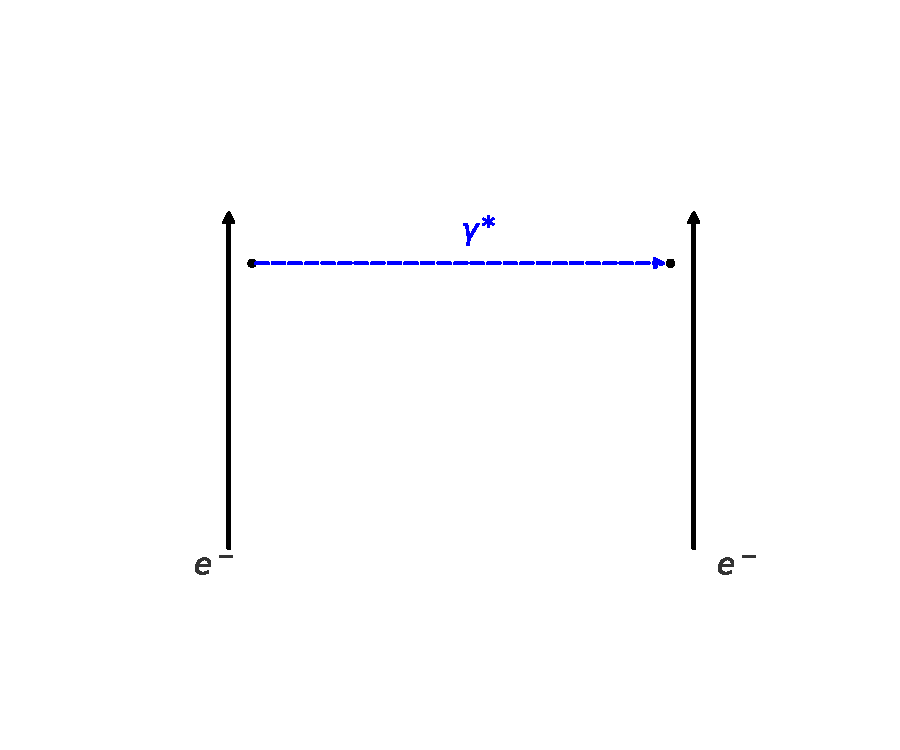
\includegraphics[width=0.4\textwidth]{bilder/moeller-diagramm.pdf}
	\end{center}
	\caption{The virtual photon is shown here as the internal line of the Feynman diagram. It transfers momentum—although it never exists as a real particle.}
\end{figure}

\subsubsection*{What Does This Diagram Show?}\index{Feynman diagrams!Interpretation}\index{Internal lines (diagrams)}\index{Vertex}\index{Momentum transfer}\index{Energy transfer}
\phantomsection
The Feynman diagram represents a typical \textbf{Møller scattering}—the elastic scattering of two electrons via the exchange of a virtual photon. The time axis runs from bottom to top.\index{Time axis (diagram)}

\begin{itemize}
	\item \textbf{Two electrons} enter the diagram from below (left and right sides). They approach each other and interact.\index{Electron}
	
	\item The \textbf{virtual photon} (depicted by the dashed blue line and the symbol $\gamma^*$) is exchanged between the electrons.\index{Photon!Virtual $\gamma^*$} It is \emph{not real}, but an intermediate state in the quantum field–theoretic calculation.\index{Intermediate state}
	
	\item The photon transfers momentum and energy—causing the electrons to change direction and leave the interaction region scattered upward.\index{Scattering angle}
	
	\item The two \textbf{vertices} (connection points) show where the interaction is localized. Mathematically, the momentum transfer takes place at these points.\index{Vertex}
\end{itemize}

\begin{tcolorbox}[didaktikbox, title=What Does the Feynman Diagram Really Show?]
	\label{box:Was zeigt das Feynman-Diagramm wirklich}
	The Møller scattering diagram does not show a real photon “flying” between electrons. Rather, it describes a quantum-mechanical intermediate state:
	
	A \textbf{virtual photon} mediates the interaction—mathematically within perturbation theory. This photon does not satisfy the classical relation $E = pc$, it exists only as an \emph{off-shell} intermediate state and transfers momentum.
	
	Real effects such as scattering angles and energy distributions can be calculated from it—without a photon ever being detected.
\end{tcolorbox}
\index{Perturbation theory}\index{Off-shell}\index{Energy distribution}

\subsubsection*{No Direct Observability—but Measurable Effect}\index{Cross section}\index{Observables}
\phantomsection
Virtual photons cannot be detected. Yet they influence measurable quantities: cross sections, scattering angles, and energy distributions can be described with high accuracy through the underlying exchange mechanism.

\subsubsection*{Distinction from Real Photon Production}\index{Compton effect}\index{Photon processes}\index{Exchange diagrams}\index{Real photons}
\phantomsection
An important difference: In the \emph{Compton effect}, a \textbf{real} photon is scattered—with detection in the experiment. In \textbf{virtual exchange}, by contrast, no photon participates as a real particle. This is the fundamental distinction between \textbf{exchange diagrams} and \textbf{photon processes}.

\vspace{1em}
\begin{tcolorbox}[didaktikbox, title=No Need for an “Invisible Force”]
	\label{box:unsichtbare Kraft}
	In quantum field theory, there is no longer a need for a classical force field acting between two charges. Instead, interactions arise through the exchange of virtual particles—in this case, virtual photons.
	
	The classical picture of action at a distance is replaced by a local, quantized exchange principle.
\end{tcolorbox}
\index{Action at a distance}\index{Locality}\index{Exchange principle}
\newpage
\noindent
\subsubsection{Feynman Diagrams as Visual Aids for Calculation}\index{Feynman diagrams!Computational aid}\index{Probability amplitude}\index{Perturbation theory}

The so-called \textbf{Feynman diagrams} are a central tool of quantum field theory—especially in Quantum Electrodynamics (QED).\index{Quantum field theory}\index{QED} They serve as a \emph{graphical notation} for mathematical terms in perturbation theory and help structure complex processes in an illustrative way.

A diagram does not represent a real “sequence in space and time,” but encodes a probability amplitude. Nevertheless, measurable physical quantities such as scattering angles, cross sections, or lifetimes can be calculated from it.\index{Lifetime}

\subsubsection*{Elements of a Feynman Diagram}\index{Fermion lines}\index{Photon lines}\index{Vertices}\index{Time axis (diagram)}
\phantomsection
\begin{itemize}
	\item \textbf{Fermion lines:} solid lines with arrows—e.g., electrons or positrons
	\item \textbf{Photon lines:} wavy or dashed lines—depending on convention
	\item \textbf{Vertices:} points where particles “interact,” i.e., momentum is transferred
	\item \textbf{Time axis:} usually bottom to top, or left to right
\end{itemize}
\begin{figure}[H]
	\begin{center}
		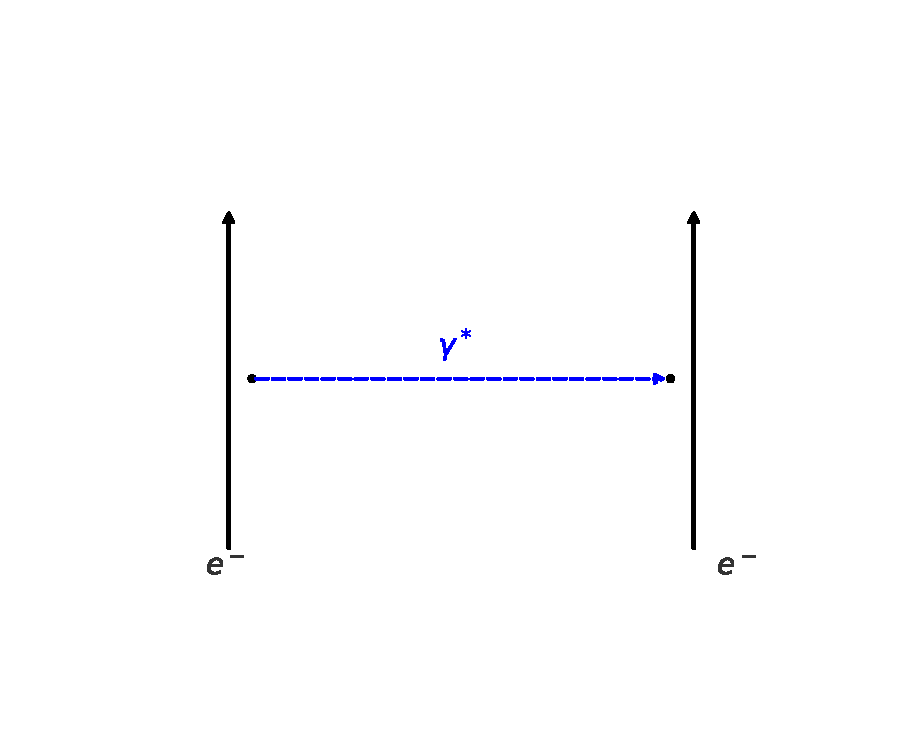
\includegraphics[width=0.45\textwidth]{bilder/feynman-einphoton.pdf}
	\end{center}
	\caption{Feynman diagram}
\end{figure}
\newpage
\noindent
\vspace{0.5em}
\begin{tcolorbox}[physikbox, title=What a Feynman Diagram Really Shows]
	\label{box:Was ein Feynman-Diagramm}
	A Feynman diagram is not a classical motion picture, but a symbolic representation of a mathematical integral over all possible paths of a process. It encodes the structure of the probability amplitude, not the exact trajectory of individual particles.
\end{tcolorbox}
\index{Path integral}

\subsubsection*{Example: Single-Photon Exchange}\index{Single-photon exchange}\index{Electron–electron scattering}\index{Momentum transfer}
\phantomsection
In elastic electron–electron scattering, the corresponding Feynman diagram consists of two incoming and two outgoing electron lines, plus one virtual photon line in between. This diagram symbolically represents a formula summing over all possible momentum transfers and times—it does not replace reality but reflects it probabilistically.\index{Probabilistic description}

\subsubsection*{More than Just Pictures—Diagram Rules}
\phantomsection
\index{Feynman rules}\index{Propagator}\index{Coupling constant}\index{Charge!Electric}\index{Amplitude!Scattering amplitude}
Every Feynman diagram corresponds to a mathematical expression. The so-called \emph{Feynman rules} assign, for example, a fraction term (propagator) to each line, a coupling constant (e.g., $e$) to each vertex, and an integral over momenta to the whole diagram. The sum of all possible diagrams up to a certain order yields the physically measurable quantity.\index{Momentum-space integral}\index{Order (perturbation theory)}

\vspace{1em}
\begin{tcolorbox}[didaktikbox, title=A Diagram Is Not Reality]
	\label{boxx:Diagramm ist nicht gleich realität}
	A common misunderstanding is that a Feynman diagram shows a real process—for example, a photon “flying.” In fact, it describes a \emph{superposition of all possible intermediate states}, summarized in a quantum-mechanical amplitude. It is therefore a computational tool, not a film of what happens.
\end{tcolorbox}
\index{Superposition}\index{Intermediate state}

\subsubsection{Illustrative Diagrams}\index{Processes!QED}\index{Virtual photons!vs.\ real photons}\index{Real photons}
\phantomsection

To better understand the role of virtual photons compared with real photons, it is worth looking at typical processes in Quantum Electrodynamics. Feynman diagrams clearly indicate whether a photon is real (detectable) or only virtual (mediating interaction).

\subsubsection*{1. Virtual Exchange: Møller Scattering (Elastic $e^-e^-$ Collision)}\index{Møller scattering}\index{Scattering!Elastic}\index{Virtual photons!Exchange}
\phantomsection
In this process, two electrons scatter elastically through the exchange of a virtual photon. The photon is not real—it only transfers momentum.\index{Momentum transfer}
\begin{figure}[H]
	\begin{center}
		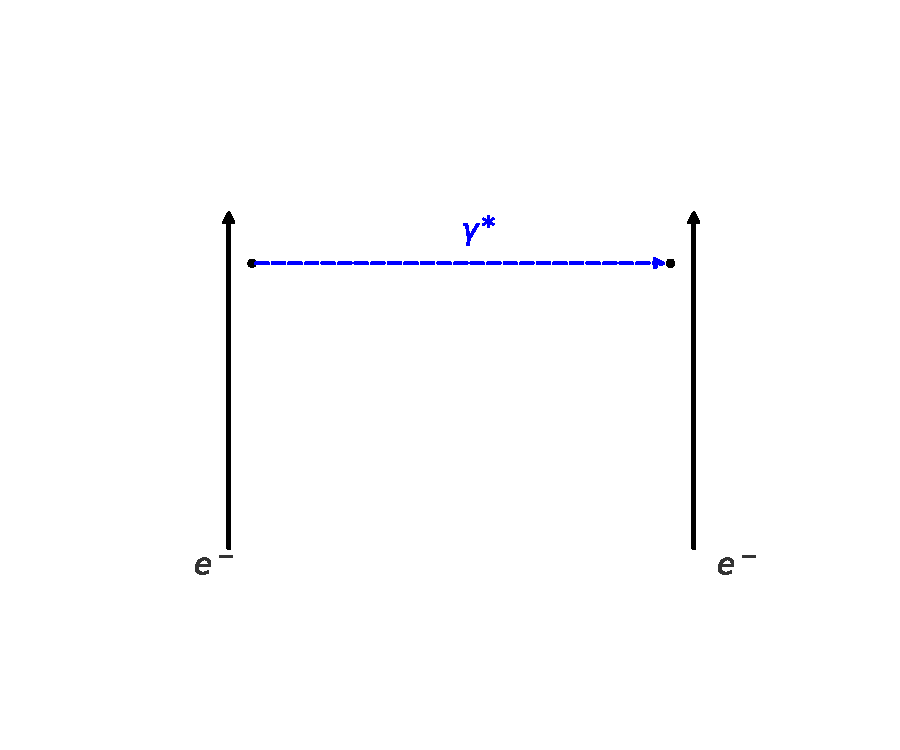
\includegraphics[width=0.42\textwidth]{bilder/moeller-diagramm.pdf}
	\end{center}
	\caption{Virtual photon}
\end{figure}

\begin{tcolorbox}[physikbox, title=Virtual Photon]
	\label{box:virtuelles Photon}
	The exchanged photon is virtual—it does not exist as a real particle. It transfers momentum and energy but does not fulfill $E = pc$.
\end{tcolorbox}
\index{Photon!Virtual}\index{Energy transfer}
\newpage
\noindent
\subsubsection*{2. Real Photon: Compton Scattering}\index{Compton effect}\index{Real photons}\index{Feynman diagrams!Compton scattering}\index{On-shell}\index{Electron propagator}\index{Vertex}
\phantomsection
In the Compton effect, a \textbf{real} photon is scattered by an electron. Both the incoming and outgoing photons are real, detectable particles.\index{Detection} The Feynman diagram shows two vertices with an internal electron propagator.\index{Propagator!Electron}\index{Vertices}

\begin{figure}[H]
	\begin{center}
		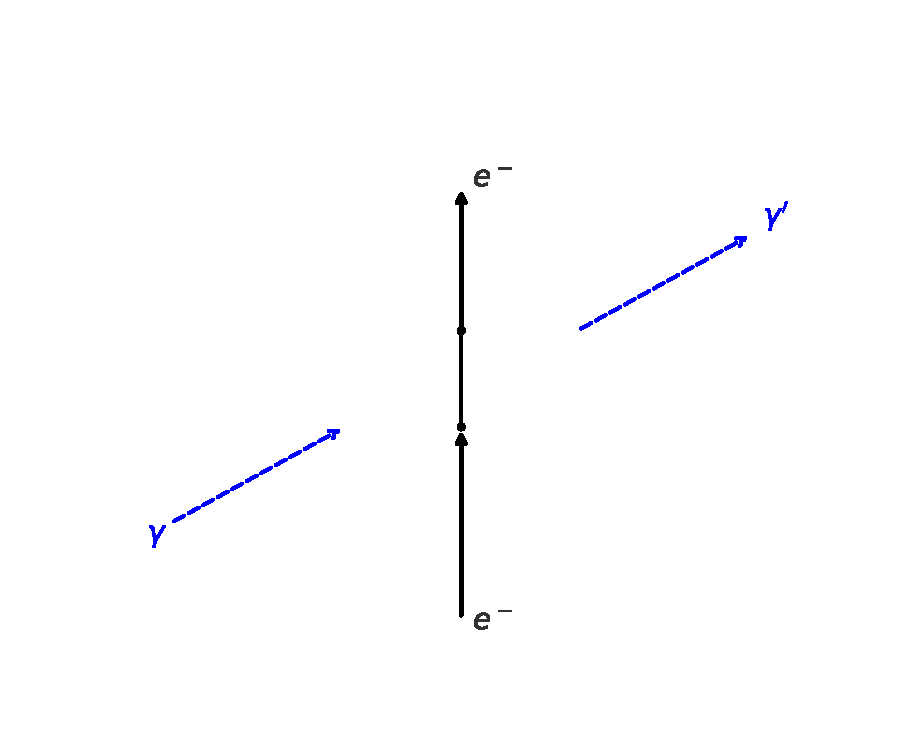
\includegraphics[width=0.5\textwidth]{bilder/compton-diagramm.pdf}
	\end{center}
	\caption{Real photon}
\end{figure}

\begin{tcolorbox}[physikbox, title=Real Photons]
	\label{box:Reale Photonen}
	In Compton scattering, photons appear as real particles. They are measurable and fulfill the on-shell condition $E = pc$.
\end{tcolorbox}
\index{Photon!Real}\index{On-shell condition}
\newpage
\noindent
\subsubsection*{3. Loop Diagrams: Self-Interaction and $g$-Factor}\index{Loop diagrams}\index{Self-energy}\index{Vertex correction}\index{g-factor!Anomaly}
\phantomsection
In higher orders of perturbation theory, closed loops appear in Feynman diagrams—for example, when an electron interacts with itself via a virtual photon.\index{Virtual photon} Such diagrams explain, among other things, the anomaly of the $g$-factor.\index{Anomaly!$g$-factor}
\begin{figure}[H]
	\begin{center}
		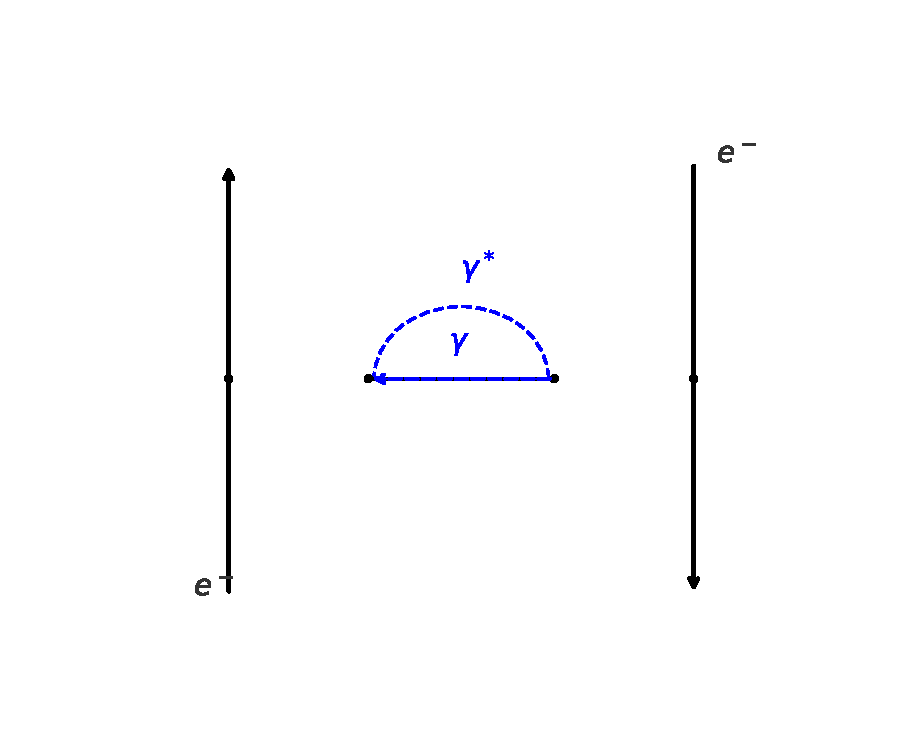
\includegraphics[width=0.4\textwidth]{bilder/vertex-korrektur.pdf}
	\end{center}
	\caption{Loop diagram}
\end{figure}

\begin{tcolorbox}[hinweisbox, title=Loop Diagrams and Precision Effects]
	\label{box:Schleifendiagramme}
	Loops with virtual photons provide corrections to simple processes—for example, for the exact value of the electron $g$-factor or the Lamb shift. These effects have been confirmed experimentally with high precision.
\end{tcolorbox}
\index{Lamb shift}\index{Precision experiments}

\subsubsection*{Didactic Comparison}\index{Didactic comparison}\index{Photons!Real vs.\ virtual}
\phantomsection
\begin{itemize}
	\item \textbf{Virtual photons} appear as internal lines in diagrams. They are not directly observable but are physically effective.\index{Internal lines}\index{Detection!Indirect}
	\item \textbf{Real photons} are external lines. They can be measured and are on-shell.\index{External lines}
\end{itemize}

\begin{tcolorbox}[didaktikbox, title=Real or Virtual Photons in the Diagram]
	\label{box:Reale oder virtuelle Photonen}
	Whether a photon is real or virtual is seen from whether it is shown as an incoming or outgoing particle. Only real photons are observable. Virtual photons are internal lines—they “exist” only within the calculation.
\end{tcolorbox}

\index{Observability}\index{Incoming particles}\index{Outgoing particles}
\newpage
\noindent
\subsubsection{Significance for QED}\index{QED!Significance}\index{Electromagnetic interaction}

Quantum Electrodynamics (QED) is the most precisely confirmed theory in physics. Its enormous accuracy would be unthinkable without the concept of virtual photons and Feynman diagrams.\index{Feynman diagrams}\index{Virtual photons}
\subsubsection*{Central Role of Virtual Photons}\index{Virtual photons!Central role}\index{Perturbation theory}
\phantomsection
Virtual photons enable the calculation of electromagnetic interaction between charged particles on the quantum level. They appear in all orders of perturbation theory—from simple exchange processes to complex loop corrections.\index{Exchange processes}\index{Loop corrections}

\vspace{1em}
\begin{tcolorbox}[physikbox, title=No QED Without Virtual Photons]
	\label{box:Ohne virtuelle Photonen keine}
	Virtual photons are the foundation of the quantum field–theoretic description of electromagnetic processes. Without them, QED could neither mediate forces nor make quantitative predictions.
\end{tcolorbox}

\subsubsection*{Feynman Diagrams as Methodological Backbone}\index{Feynman diagrams!Method}\index{Amplitudes!Probability}
\phantomsection
Feynman diagrams provide not only an illustrative representation but also a precise computational prescription. For every possible interaction, all allowed diagrams can be drawn and translated into a mathematical expression. The sum of all diagrams yields the observable amplitude.\index{Sum over diagrams}

\subsubsection*{Example: Calculation of the $g$-Factor}\index{g-factor!Electron}\index{Anomalous magnetic moment}
\phantomsection
The deviation of the electron’s gyromagnetic factor from the classical value $g = 2$ is one of the most accurate experiments in modern physics. The correction arises from a loop process with a virtual photon—that is, from a second-order Feynman diagram.\index{Second order}

\subsubsection*{Accuracy of the Theory}\index{QED!Accuracy}\index{Theory–experiment comparison}
\phantomsection
The theoretically calculated values for quantities such as the Lamb shift, the electron $g$-factor, or scattering angles in electron collisions agree with measurements to many decimal places.\index{Scattering angle}\index{Electron scattering}

\vspace{1em}
\begin{tcolorbox}[didaktikbox, title=Quantum Electrodynamics as a Success Story]
	\label{box:Die Quantenelekrodynamik}
	QED is not only an elegant theory—it delivers, with the help of virtual particles and Feynman diagrams, quantitative predictions with an accuracy of up to 12 decimal places. The role of the photon—even as a virtual particle—is central.
\end{tcolorbox}
\index{Success story}\index{Accuracy!12 decimal places}

\subsubsection{Limits and Misconceptions}\index{Limits of QED}\index{Misconceptions!Feynman diagrams}

Despite their illustrative representation, Feynman diagrams must not be misunderstood as pictorial descriptions of real processes. Virtual photons do not exist in the classical sense—they are mathematical objects within an approximation method.\index{Approximation method}

\subsubsection*{Virtual Photons Do Not Fly}\index{Virtual photons!Do not fly}\index{Particle trajectory!Not classical}
\phantomsection
It is misleading to say that a virtual photon “flies back and forth between two electrons.” Virtual particles are not measurable, not localized, and do not satisfy a classical equation of motion. Their role consists exclusively in mediating interaction within a quantum-mechanical computational model.\index{Localization}\index{Equation of motion!Classical}

\vspace{0.5em}
\begin{tcolorbox}[didaktikbox, title=No Particle Trajectory in the Diagram]
	\label{box: Keine Teilchenbahn im Diagramm}
	A Feynman diagram does not describe motion in space or a classical flight path. It represents a symbolic structure for calculating an amplitude. The “lines” in the diagram are not trajectories but terms in a formula.
\end{tcolorbox}
\index{Lines!Not trajectories}

\subsubsection*{Off-Shell Means: No Energy–Momentum Relation}\index{Off-shell}\index{Energy–momentum relation}
\phantomsection
Virtual photons do not satisfy the familiar relation $E = pc$. They are \emph{off-shell}, i.e., they temporarily violate the energy–momentum balance—within the framework of Heisenberg’s uncertainty relation.\index{Uncertainty principle!Time–energy} This is not a weakness of the theory but one of its central features.

\subsubsection*{Diagrams Are Not Exact Pictures}\index{Feynman diagrams!Not pictures}\index{Reality!vs.\ Model}
\phantomsection
Another misconception is to assume that Feynman diagrams show “what really happens.” In fact, they contain no statement about the sequence of events, real locations, or classical times. The diagrams represent probability amplitudes—not observations.\index{Observations}

\vspace{0.5em}
\begin{tcolorbox}[warnbox, title=Warning: Do Not Take Feynman Diagrams Literally!]
	\label{box:Warnung}
	Feynman diagrams are a powerful computational tool—but not sketches of reality. Interpreting them as “sequences of particle flights” misses the essence of quantum field theory.
\end{tcolorbox}
\index{Warning}

\subsubsection*{Limits of Validity}\index{Range of validity}\index{Strong interaction!Limits of perturbation theory}\index{Lattice gauge theory}
\phantomsection
QED—and with it the concept of virtual photons—is a perturbation theory. It works excellently for small coupling constants (e.g., in electrodynamics), but fails for strong interactions. There, other methods (e.g., lattice theory) are required.

\subsubsection*{Conclusion of This Section}\index{Conclusion!Virtual photons and diagrams}
\phantomsection
Virtual photons and Feynman diagrams are central concepts in QED—but they must be interpreted correctly: not as “flying particles” but as building blocks of a mathematical theory with enormous predictive power.

\subsubsection{Summary}\index{Summary!QED interpretation}

Virtual photons do not appear in detectors—but they determine what is measured there. They are the invisible carriers of electromagnetic interaction in the quantum world. Feynman diagrams help capture their effect mathematically, without attributing to them a classical reality.

QED would not be possible without these concepts—and it is precisely these seemingly abstract building blocks that make it the most precise theory in physics.\index{Most precise theory}

\subsection{The QED Formalism}\index{QED!Formalism}\index{Lagrangian density!QED}\index{Gauge invariance}\index{Renormalization@Renormalization (general)}
% Coupling constant, gauge invariance, renormalization, propagators

Quantum Electrodynamics—QED for short—is the field theory of the electromagnetic interaction.\index{Field theory} It describes how electrons, positrons, and photons behave quantum mechanically and interact with each other.\index{Electron}\index{Positron}\index{Photon}

In the previous chapter we saw how Feynman diagrams are used to represent processes such as electron scattering, the Compton effect, or self-interactions.\index{Electron scattering}\index{Compton effect}\index{Self-interaction} But these diagrams are not a substitute for the underlying theory—they are \emph{derived tools}.\index{Tools!Derived}

In this chapter, we go one step deeper: we look at the \textbf{mathematical structure} of QED.\index{Mathematical structure} At the center is the so-called \textbf{Lagrangian density}, from which all predictions of the theory can be derived—from the structure of the interaction to the Feynman rules.\index{Feynman rules}

It turns out: The whole of Quantum Electrodynamics can be built from just a few principles—especially the requirement of \textbf{gauge invariance} and of \textbf{relativity}.\index{Relativity} These principles determine not only the form of the equations but also how the photon fits into the theory as a massless interaction particle.\index{Photon!Massless}\index{Interaction particle}

The goal of this chapter is therefore to understand QED from its foundations—not as a collection of computational rules, but as an elegantly structured theory with enormous predictive power.\index{Predictive power}

\vspace{1em}
\begin{tcolorbox}[hinweisbox, title=Note for Readers]
	\label{box:Hinweis füe Leser}
	This chapter introduces the mathematical structure of Quantum Electrodynamics (QED). It is aimed at readers interested in the theoretical derivation of photon interaction. 
	
	Readers primarily interested in experimental confirmation and applications may skip directly to Chapter~5.5—without losing the main thread of the book.
\end{tcolorbox}


\subsubsection{Basic Idea of QED as a Field Theory}\index{Basic idea!QED}\index{Field theory!Basics}

Quantum Electrodynamics is a \textbf{field theory}.\index{Field theory} This means: it does not describe individual particles but fields that propagate through space and interact with each other.

An electron is not treated as a point particle but as an excitation of a \emph{Dirac field}.\index{Dirac field} Light—or more precisely: the photon—is likewise neither a wave nor a classical particle, but the excitation of an \emph{electromagnetic field}, which itself is quantized.\index{Electromagnetic field!Quantized}

\subsubsection*{Particles as Fields}\index{Particles as fields}\index{Fock space}\index{Excitations}
\phantomsection
Instead of describing the exchange of particles, QED works with fields such as:
\begin{itemize}
	\item \textbf{Electron field} $\psi(x)$ (Dirac field)\index{Electron field $\psi$}
	\item \textbf{Photon field} $A^\mu(x)$ (Four-potential)\index{Photon field $A^\mu$}\index{Four-potential}
\end{itemize}

The state of an electron (e.g., position, momentum, spin) is described by a wave function within the Dirac field.\index{Wave function}\index{Spin} A photon, on the other hand, is an excitation of the quantized field $A^\mu$—more precisely: a \textbf{Fock state} with one photon.\index{Fock state}

\subsubsection*{Interaction Through Coupling of Fields}\index{Interaction!Field coupling}
\phantomsection
The central idea of QED is that these two fields are \emph{coupled} to each other. The interaction does not take place directly between particles, but through terms in the so-called \textbf{Lagrangian density}:\index{Lagrangian density}
\[
\mathcal{L}_{\text{int}} = -e \, \bar{\psi} \gamma^\mu \psi \, A_\mu
\]
\index{Coupling term $-e\bar\psi\gamma^\mu\psi A_\mu$}

This expression describes that the electron field $\psi$ couples to the electromagnetic field $A_\mu$—in other words, it “feels” the presence of a photon.\index{Coupling!Electron–photon} The coupling term contains exactly the structure that later appears in Feynman diagrams as a vertex.\index{Vertex}

\vspace{0.5em}
\begin{tcolorbox}[physikbox, title=Field Theory Instead of Particle Mechanics]
	\label{box:Feldtheorie statt Teilchenmechanik}
	In QED, electrons and photons are not treated as classical particles but as quantized fields. Their interaction arises from a coupling term in the Lagrangian density—not from a classical force.
\end{tcolorbox}
\index{Particle mechanics!vs.\ Field theory}

\subsubsection*{Why This Approach Is Necessary}\index{Motivation!QED}\index{Limits!Classical electrodynamics}
\phantomsection
Classical electrodynamics (Maxwell’s equations) cannot explain many phenomena:\index{Maxwell’s equations}
\begin{itemize}
	\item No quantized energy transfer\index{Energy transfer!Quantized}
	\item No concept of the photon\index{Photon!Concept}
	\item No way to describe scattering at the quantum level\index{Scattering!Quantum level}
\end{itemize}

Only a quantized field theory makes it possible to describe processes such as the photoelectric effect, Compton scattering, or electron–positron annihilation correctly.\index{Photoelectric effect}\index{Compton effect}\index{Annihilation!Electron–positron}
\newpage
\noindent
\vspace{0.5em}
\begin{tcolorbox}[didaktikbox, title=Why Not Simply Classical?]
	\label{box:Warum nicht einfach klassisch?}
	Quantum field theory extends quantum mechanics to systems with variable particle number. Only in this way can creation and annihilation of photons or electrons be described rigorously. Without this approach, one could not derive Feynman diagrams—nor achieve the precision results of QED.
\end{tcolorbox}
\index{Quantum field theory}\index{Quantum mechanics}\index{Creation and annihilation}

\subsubsection{The QED Lagrangian Density}\index{Lagrangian density!QED}

At the heart of QED is the so-called \textbf{Lagrangian density}, from which all equations of the theory can be derived. It contains both the free fields (electron, photon) and their interaction.

The full QED Lagrangian density reads:
\[
\mathcal{L}_{\text{QED}} = \bar{\psi}(i \gamma^\mu \partial_\mu - m)\psi - \frac{1}{4}F_{\mu\nu}F^{\mu\nu} - e \bar{\psi} \gamma^\mu \psi A_\mu
\]

\begin{tcolorbox}[mathebox, title=Structure of the QED Lagrangian Density]
	\label{box:Sufbau der QED-Langrangedichte}
	\begin{itemize}
		\item $\bar{\psi}(i \gamma^\mu \partial_\mu - m)\psi$: Dirac term for the free electron field\index{Dirac term}
		\item $-\frac{1}{4}F_{\mu\nu}F^{\mu\nu}$: Kinetic term for the photon (Maxwell part)\index{Maxwell term}\index{Kinetic term}
		\item $-e \bar{\psi} \gamma^\mu \psi A_\mu$: Coupling between electron field and electromagnetic field\index{Coupling!Electron–photon}
	\end{itemize}
\end{tcolorbox}

\subsubsection*{Meaning of the Terms}\index{Interpretation of terms}\index{Free field}
\phantomsection
Each part of the Lagrangian density corresponds to a component of the theory:

- The first term describes the \textbf{free Dirac field}—that is, an electron or positron without external influence.\index{Free Dirac field}
- The second term is the \textbf{free electromagnetic field strength}—the quantum version of the Maxwell field.\index{Free photon field}
- The third term describes the \textbf{interaction} between electron and photon—the core of QED.\index{Interaction!Electron–photon}

\subsubsection*{Field Strength Tensor}\index{Field strength tensor $F_{\mu\nu}$}
\phantomsection
The expression $F_{\mu\nu}$ is the so-called \textbf{field strength tensor}, defined as:
\[
F_{\mu\nu} = \partial_\mu A_\nu - \partial_\nu A_\mu
\]
\index{Lorentz invariance}

It contains both the electric and the magnetic field—packaged into a single relativistic object. The term $F_{\mu\nu}F^{\mu\nu}$ is invariant under Lorentz transformations.

\vspace{1em}
\begin{tcolorbox}[physikbox, title=Photon Field from the Lagrangian Density]
	\label{box:Photonenfeld aus der Lagrangedichte}
	The photon’s quantum nature arises in QED from the quantization of the field $A^\mu$ within the Maxwell structure. The field strength tensor $F_{\mu\nu}$ contains the dynamics of the photon as a quantized gauge field.
\end{tcolorbox}
\index{Gauge field}

\subsubsection*{Interaction as Coupling Terms}\index{Interaction!Coupling terms}\index{QED vertex}
\phantomsection
The interaction term\\$-e \bar{\psi} \gamma^\mu \psi A_\mu$ describes the coupling of electrons to the photon. 

From this term follows directly the structure of the QED vertex in Feynman diagrams:
\begin{figure}[H]
	
	\[
	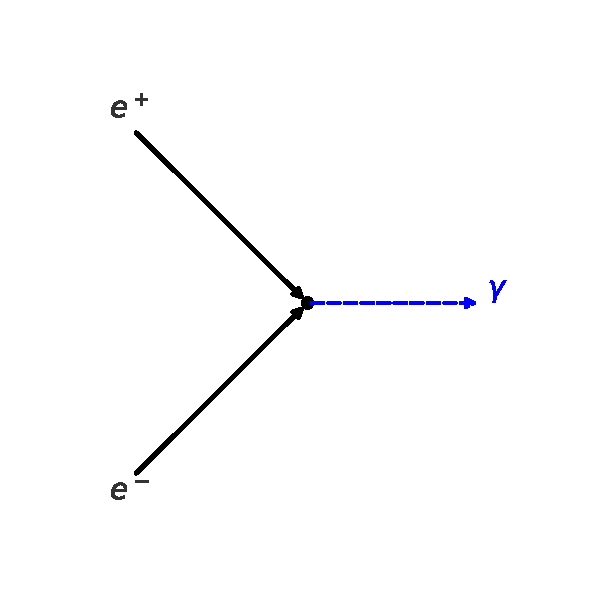
\includegraphics[height=8.5em]{bilder/qed-vertex.pdf} \quad \Rightarrow \quad -ie\gamma^\mu
	\]
	\caption{Interaction term}
\end{figure}
\vspace{0.5em}
\begin{tcolorbox}[didaktikbox, title=From Lagrangian Term to Feynman Vertex]
	\label{box:Vom Lagrange-Term zum Feynmann-Vertax}
	The coupling in the Lagrangian density generates the QED vertex: one electron, one positron, one photon meet at a point. This structure forms the basis of all diagrams in QED.
\end{tcolorbox}
\index{Vertex factor $-ie\gamma^\mu$}
\subsubsection*{Gauge Invariance as a Principle}\index{Gauge invariance!Local}\index{Gauge transformation}
\phantomsection
The form of the QED Lagrangian density is not chosen arbitrarily. It results from the requirement that the theory be \textbf{locally gauge invariant}—that is, symmetric under transformations of the form:
\[
\psi(x) \rightarrow e^{i\alpha(x)} \psi(x), \qquad A_\mu(x) \rightarrow A_\mu(x) - \frac{1}{e} \partial_\mu \alpha(x)
\]

Only with this structure does the theory remain consistent, relativistically invariant, and quantizable.\index{Quantizability}

\subsubsection{Coupling Between Electrons and Photons}\index{Coupling!Electron–photon}\index{Local gauge invariance}

In QED, the interaction between electron and photon does not arise “from the outside,” but follows from a fundamental principle: \textbf{local gauge invariance}. This symmetry forces us to introduce the photon as the coupling partner of the electron field.

\subsubsection*{Global and Local Phase Transformations}\index{Phase transformation!Global}\index{Phase transformation!Local}
\phantomsection
A Dirac field $\psi$ is invariant under a \textbf{global} phase transformation:
\[
\psi(x) \rightarrow e^{i\alpha} \psi(x)
\]
The Lagrangian density remains unchanged—this is a symmetry.

If, however, one demands that $\alpha$ depends on position, i.e.
\[
\psi(x) \rightarrow e^{i\alpha(x)} \psi(x)
\]
one speaks of a \textbf{local gauge transformation}. This destroys the invariance of the Lagrangian density—unless one introduces an additional field $A_\mu(x)$ that co-transforms:
\[
A_\mu(x) \rightarrow A_\mu(x) - \frac{1}{e} \partial_\mu \alpha(x)
\]

\subsubsection*{Covariant Derivative and Minimal Substitution}\index{Covariant derivative}\index{Minimal substitution}
\phantomsection
To keep the theory locally gauge invariant, one replaces the ordinary derivative in the Dirac Lagrangian by the \textbf{covariant derivative}:
\[
\partial_\mu \rightarrow D_\mu = \partial_\mu + ie A_\mu
\]

This automatically generates an interaction term in the Lagrangian density:
\[
\mathcal{L}_{\text{int}} = -e \, \bar{\psi} \gamma^\mu \psi A_\mu
\]

\vspace{0.5em}
\begin{tcolorbox}[mathebox, title=Coupling From Principle]
	\label{box:Kopplung aus Prinzip}
	The coupling between electron and photon is not an added term, but follows necessarily from the demand for local gauge invariance. It uniquely determines the form of the interaction.
\end{tcolorbox}
\index{Four-current density $\bar\psi\gamma^\mu\psi$}

\subsubsection*{Physical Meaning}\index{Physical meaning!Coupling}
\phantomsection
The expression $\bar{\psi} \gamma^\mu \psi$ is the \textbf{four-current density} of the electron field. The term $A_\mu$ couples to this current—exactly as a classical electromagnetic field couples to an electric current. The difference is that here both quantities are quantized.\index{Current!Electric}

\subsubsection*{Simple Picture: “Field Feels Field”}\index{Illustrative picture}\index{Field–field coupling}
\phantomsection
One can picture the process as follows: The electron field “feels” the photon field—because its derivative is modified. Where formerly only the gradient appeared, there is now a term that includes the photon as well.

\vspace{1em}
\begin{tcolorbox}[didaktikbox, title=The Force Arises From the Derivative]
	\label{box:Die Kraft entsteht aus dem Ableiter}
	In QED, the electromagnetic interaction arises because the electron field responds to the \emph{covariant} derivative. This derivative contains the photon—and with it, the coupling is generated.
\end{tcolorbox}
\index{Force!Origin in $D_\mu$}

\subsubsection{Feynman Rules From the Lagrangian Density}\index{Feynman rules}\index{Perturbation theory}

Feynman diagrams are not mere sketches—they follow from the structure of the Lagrangian density. Each term in the QED Lagrangian density has a clear correspondence to a building block of the diagrams.

\subsubsection*{Basic Principle: Perturbative Expansion}\index{Perturbative expansion}\index{Fine-structure constant $\alpha$}
\phantomsection
Since the interaction in QED is weak (the fine-structure constant $\alpha \approx 1/137$ is small), physical quantities such as transition probabilities or scattering amplitudes can be expanded as a \textbf{series in the coupling constant}. Each term in this series corresponds to a Feynman diagram.\index{Transition probability}\index{Scattering amplitude}

\subsubsection*{Elements and Their Meaning}\index{Propagator}\index{Vertex}\index{Momentum integral}
\phantomsection
From the Lagrangian density, the following correspondences emerge:

\vspace{0.5em}
\begin{tcolorbox}[mathebox, title=Feynman Rules of QED (Simplified)]
	\label{box:Feynman-Regeln der QED}
	\begin{itemize}
		\item \textbf{Electron line:} $\displaystyle \frac{i(\slashed{p} + m)}{p^2 - m^2 + i\varepsilon}$ (Dirac propagator)\index{Dirac propagator}
		\item \textbf{Photon line:} $\displaystyle \frac{-ig^{\mu\nu}}{q^2 + i\varepsilon}$ (Photon propagator)\index{Photon propagator}
		\item \textbf{Vertex:} $-ie\gamma^\mu$\index{Vertex factor $-ie\gamma^\mu$}
		\item \textbf{Each internal line:} Integration over four-momentum $d^4p$\index{Four-momentum!Integration}
		\item \textbf{Complete diagram:} Product of all factors, integration over loop momenta\index{Loop momentum}
	\end{itemize}
\end{tcolorbox}

\subsubsection*{Example: Single-Photon Exchange}\index{Single-photon exchange}\index{Møller scattering}
\phantomsection
The simplest application is Møller scattering (electron–electron scattering via a virtual photon). From the vertex $-ie\gamma^\mu$ and the propagators, the formula for the scattering amplitude results. The calculation follows directly from the Feynman rules—and yields measurable quantities such as cross sections and scattering angles.\index{Cross section}

\subsubsection*{Order of the Diagrams}\index{Order!in $e$}\index{Order!in $\alpha$}\index{Loop corrections}
\phantomsection
The more vertices a diagram contains, the higher its order in $e$ or in $\alpha = e^2 / (4\pi\hbar c)$. Lower orders yield the main contributions, higher orders the corrections—in the form of loops (loop corrections).

\vspace{1em}
\begin{tcolorbox}[didaktikbox, title=Why the Rules Work]
	\label{box:Warum die Regeln funktionieren}
	The Feynman rules arise systematically from the QED Lagrangian density by applying perturbation theory. They are therefore not a collection of arbitrary instructions—but the direct result of the structure of the theory.
\end{tcolorbox}

\subsubsection*{Connection to Measurement}\index{Measurement!Connection}\index{Theory–experiment}
\phantomsection
Every observable quantity—scattering angle, energy distribution, $g$-factor correction—can be calculated using the Feynman rules. The agreement with experiment makes QED the most precise theory in physics.\index{Energy distribution}

\subsubsection{Quantization of the Electromagnetic Field}\index{Quantization!Electromagnetic field}\index{Photon!As excitation}

In classical electrodynamics, the electromagnetic field is described by the four-potential $A^\mu(x)$. But as long as this field only satisfies classical equations (e.g., Maxwell’s equations), there are no photons. Only through \textbf{quantization} does the field become a quantum system—and the photon appears as an \emph{excitation} of this field.\index{Maxwell’s equations}

\subsubsection*{From Wave to Photon}\index{Modes!Quantization}\index{Fock space}
\phantomsection
The electromagnetic field consists of infinitely many oscillating degrees of freedom—similar to a guitar string with infinitely many possible overtones. Each mode can be quantized. In this way, a \textbf{Fock space} arises, describing states such as
\[
\lvert 0 \rangle, \quad \lvert 1_{\vec{k}} \rangle, \quad \lvert 2_{\vec{k}} \rangle, \quad \dots
\]
—that is, states with zero, one, or several photons of a given wave number $\vec{k}$.\index{Vacuum state}\index{Photon number state}

\subsubsection*{The Photon as Excitation}\index{Photon!Quantum state}\index{Momentum $\hbar\vec{k}$}\index{Energy $\hbar\omega$}
\phantomsection
A photon is nothing more than a state with a single excitation of the quantized field $A^\mu(x)$ in a particular mode. This perspective is fundamentally different from the classical view of a wave or particle.

\vspace{0.5em}
\begin{tcolorbox}[physikbox, title=What Is a Photon in QED?]
	\label{box:Warum ist ein Photon in der QED}
	A photon is the simplest excitation of the quantized electromagnetic field. It has no rest mass, but a definite energy $E = \hbar \omega$ and momentum $\vec{p} = \hbar \vec{k}$.
\end{tcolorbox}

\subsubsection*{Polarization and Transversality}\index{Polarization}\index{Transversality}\index{Helicity}
\phantomsection
Because the photon is massless, it has only two physically observable polarization states—not three, as a massive spin-1 particle would have. This is a direct consequence of gauge invariance and the transversality condition:
\[
\vec{k} \cdot \vec{\epsilon} = 0
\]

QED handles this correctly via the \textbf{Gupta–Bleuler formalism}\index{Gupta–Bleuler formalism} or through Feynman gauges, in which unphysical degrees of freedom are carried along at first and later canceled.\index{Feynman gauge}

\subsubsection*{Gauge Symmetry and Degrees of Freedom}\index{Gauge symmetry}\index{Degrees of freedom}
\phantomsection
Gauge symmetry makes it possible to eliminate certain components of the field $A^\mu$ through transformations. Only the transverse components remain physically relevant—and these are precisely the two polarization directions of the photon.

\vspace{1em}
\begin{tcolorbox}[didaktikbox, title=Why Doesn’t the Photon Have a Spin-3 State?]
	\label{box:Warum hat das Photon keinen Spin-3-Zustand}
	A massive spin-1 particle would have three polarization states. But because the photon is massless and the electromagnetic field is gauge invariant, only two states remain. These correspond to linear or circular polarization.
\end{tcolorbox}
\index{Spin!Photon}\index{Circular polarization}\index{Linear polarization}

\subsubsection{Summary}\index{Summary!QED formalism}
\addcontentsline{toc}{subsubsection}{Summary}

Quantum Electrodynamics (QED) is the quantized field theory of electromagnetic interaction. Its mathematical structure rests on the following key elements:

\begin{itemize}
	\item \textbf{Field description:} Electrons and positrons are described by the Dirac field $\psi(x)$, the photon by the four-potential $A^\mu(x)$.\index{Dirac field}\index{Four-potential}
	\item \textbf{Lagrangian density:} The QED Lagrangian density contains three components:
	\begin{itemize}
		\item the free Dirac term for the electron field,\index{Dirac term}
		\item the free Maxwell term for the photon field (field strength tensor $F_{\mu\nu}$),\index{Maxwell term}\index{Field strength tensor $F_{\mu\nu}$}
		\item and the coupling term $-e \bar{\psi} \gamma^\mu \psi A_\mu$.\index{Coupling term $-e\bar\psi\gamma^\mu\psi A_\mu$}
	\end{itemize}
	\item \textbf{Coupling via gauge symmetry:} The form of the interaction term follows from the requirement of local gauge invariance. It requires the introduction of a covariant derivative.\index{Covariant derivative}
	\item \textbf{Feynman rules:} From the Lagrangian density, the building blocks of Feynman diagrams can be derived: propagators, vertices, and integration rules.\index{Propagator}\index{Vertex}\index{Integration rules}
	\item \textbf{Quantization of the photon field:} By quantizing the electromagnetic field, photons emerge as excitations—with two physical polarization states.\index{Quantization!Photon field}\index{Polarization!Photon}
\end{itemize}

QED is internally consistent, relativistically invariant, and agrees with experimental reality in all tested domains.\index{Consistency}\index{Lorentz invariance} The explicit calculation of physical quantities proceeds via perturbation series and Feynman diagrams—this is the subject of the next chapter.\index{Perturbation series}

\subsection{Precision Experiments}\index{Precision experiments}\index{Tests!QED}

This section highlights the role of the photon in modern high-precision experiments.\index{Photon!Role in experiments} Such experiments provide not only impressive confirmations of Quantum Electrodynamics (QED), but also of special relativity and fundamental symmetries of nature.\index{Special relativity}\index{Symmetries!Fundamental} The photon is not only an object of observation but often also the central tool for probing the finest physical effects.\index{Photon!Measuring tool}

\subsubsection{The Anomalous Magnetic Moment of the Electron}\index{Magnetic moment!Anomalous}\index{g-factor!Electron}

One of the most accurately tested results of QED is the so-called \emph{anomalous magnetic moment} of the electron, i.e.\ the tiny deviation of the $g$-factor from exactly 2:
\[
g_e \approx 2.00231930436...
\]
This deviation results from quantum field–theoretic corrections, in particular from the exchange of virtual photons:\index{Corrections!Quantum field theory}\index{Virtual photons!Loops}
\vspace{1em}
\begin{tcolorbox}[physikbox,title=Physical Meaning]
	\label{box:physikalische Bedeutung}
	The difference between $g_e = 2$ and the experimentally measured value is explained by loop processes in Feynman diagrams, in which virtual photons mediate between the electron and itself. The agreement between theory and experiment is a triumph of QED.
\end{tcolorbox}
\index{Triumph of QED}

\subsubsection{Lamb Shift}\index{Lamb shift}\index{Hydrogen!Spectrum}

Another spectacular example of experimental confirmation of QED is the \emph{Lamb shift} of the energy levels in the hydrogen atom. The classical Dirac formalism predicts the same energy for the 2s and 2p levels. Experimentally, however, a tiny energy shift was found:
\[
\Delta E_\text{Lamb} \approx \SI{1057}{\mega\hertz}
\]
\vspace{0.5em}
\begin{tcolorbox}[didaktikbox,title=Why Is This Important?]
	\label{box:Warum ist wichtig}
	The Lamb shift shows that empty space—the quantum vacuum—is not “empty.” Virtual photons cause fluctuations that influence the energy levels.
\end{tcolorbox}
\index{Quantum vacuum}\index{Vacuum fluctuations}

\subsubsection{Spectroscopy and Constant Measurements}\index{Spectroscopy}\index{Fundamental constants!Measurements}\index{Frequency comb}\index{Atomic clock}

Photon-based high-precision spectroscopy also provides the most accurate measurements of fundamental constants such as:

\begin{itemize}
	\item the fine-structure constant $\alpha$\index{Fine-structure constant $\alpha$}
	\item Planck’s constant $h$\index{Planck’s constant $h$}
	\item the speed of light $c$ (now fixed by definition)\index{Speed of light $c$}
\end{itemize}

These measurements rely on laser technology, frequency combs, and atomic clocks—all photon-based techniques.\index{Laser}\index{Photon technologies}

\subsubsection{Tests of Fundamental Symmetries}\index{Symmetries!Tests}\index{CPT invariance}\index{Lorentz invariance}

Photon experiments also contribute to testing fundamental symmetries:

\begin{itemize}
	\item \textbf{CPT invariance:} Precision measurements on antihydrogen compare spectral lines with ordinary hydrogen.\index{Antihydrogen}
	\item \textbf{Lorentz invariance:} Directional dependence of the speed of light is tested with resonator-based laser systems.\index{Resonator!Optical}
\end{itemize}
\vspace{0.5em}
\begin{tcolorbox}[hypobox, title={What If Light Were Not Isotropic?}]
	\label{box:was wäre nicht isotop}
	If a directional dependence of the speed of light were measured, it would indicate a fundamental violation of Lorentz symmetry—with drastic consequences for relativity and our physical worldview.
\end{tcolorbox}
\index{Isotropy of light}\index{Lorentz symmetry!Violation}

\subsubsection{Summary}\index{Summary!Precision experiments}

Precision experiments are among the strongest pillars for testing our physical theories. They show how deeply anchored and reliable the concept of the photon is in modern physics. In particular, Quantum Electrodynamics demonstrates here its unparalleled accuracy—with the photon as both exchange particle
\subsubsection{Summary}\index{Summary!Precision experiments}

Precision experiments are among the strongest pillars for testing our physical theories. They show how deeply anchored and reliable the concept of the photon is in modern physics. In particular, Quantum Electrodynamics demonstrates its unparalleled accuracy—with the photon as both \emph{exchange particle} and \emph{information carrier}.\index{Exchange particle}\index{Information carrier!Photon}

\subsection{Conclusion}\index{Conclusion}

In Chapter~V we have encountered the photon as the central mediator of the electromagnetic interaction within Quantum Electrodynamics (QED).\index{Mediator} Beginning with the transition from the classical light quantum to the quantized field, it became clear how deeply the structure of QED is intertwined with the photon.

We have seen:
\begin{itemize}
	\item how the photon can be described mathematically as a vector field with gauge freedom,\index{Vector field!Photon}\index{Gauge freedom}
	\item how virtual photons in Feynman diagrams mediate the interaction between charged particles,\index{Virtual photons!Mediation}
	\item how the QED formalism is built from gauge symmetry, Lagrangian density, and perturbation theory,\index{QED!Structure}\index{Perturbation theory}
	\item and how precision experiments—from the $g$-factor to the Lamb shift—confirm the theory with unprecedented accuracy.\index{Confirmation!Experimental}
\end{itemize}

QED ranks among the most successful theories in physics. It not only delivers precise predictions, but also a deep understanding of the role of the photon—as a massless yet powerful quantum object.\index{Quantum object!Photon}

\vspace{1em}
\begin{tcolorbox}[hinweisbox,title=Outlook to Chapter VI]
	\label{box:Ausblick auf Kapitel 6}
	In the next chapter we explore applications of the photon in practice and research—from laser technology to quantum sensors and the role of photons in modern communication.
\end{tcolorbox}
\index{Laser technology}\index{Quantum sensing}\index{Quantum communication}


	\chapter{Applications of the Photon}

\setcounter{section}{6}
\setcounter{subsection}{0}
\setcounter{subsubsection}{1}
\setcounter{secnumdepth}{3}
% Define box styles
\tcbset{physikbox/.style={colback=blue!5!white, colframe=blue!75!black, fonttitle=\bfseries}}
\tcbset{mathebox/.style={colback=green!5!white, colframe=green!50!black, fonttitle=\bfseries}}
\tcbset{didaktikbox/.style={colback=yellow!5!white, colframe=yellow!50!black, fonttitle=\bfseries}}
\tcbset{hypobox/.style={colback=orange!5!white, colframe=orange!75!black, fonttitle=\bfseries}}
\tcbset{hinweisbox/.style={colback=gray!10!white, colframe=black!40!black, fonttitle=\bfseries}}

\subsection{Introduction}

Photons\index{Photon} are not only fundamental carriers of quantum-physical properties\index{Quantum-Physical Property} – they also form the basis of countless applications\index{Application} in technology\index{Technology}, research\index{Research}, and everyday life.  
This chapter presents selected fields of use where the control\index{Photon Control}, detection\index{Photon Detection}, and utilization\index{Photon Utilization} of individual photons play a central role.  
The range extends from laser technology\index{Laser Technology} and quantum sensing\index{Quantum Sensing} to medical imaging\index{Medical Imaging}, optical communication\index{Optical Communication}, and astronomical observation\index{Astronomical Observation}.  
The goal is to make the physical principles\index{Physical Principle} behind these applications understandable and to show their significance for science\index{Science} and society.\index{Society}

\subsection{Photons in Laser Technology}
\subsubsection{Operating Principle of Lasers}

The term “laser”\index{Laser} stands for \textbf{Light Amplification by Stimulated Emission of Radiation}\index{Light Amplification by Stimulated Emission of Radiation}.  
A laser does not produce light\index{Light} through incandescence\index{Incandescence} or chemical reactions\index{Chemical Reaction}, but by the controlled amplification of photons in an active medium\index{Active Medium} – based on the principle of \emph{stimulated emission}\index{Stimulated Emission}.

\noindent
The three central processes\index{Einstein Processes}, theoretically described by Einstein\index{Einstein, Albert} already in 1916, are:

\begin{itemize}
	\item \textbf{Spontaneous emission}\index{Spontaneous Emission}: An excited atom\index{Atom} decays to a lower state without external influence and emits a photon.
	\item \textbf{Absorption}\index{Absorption}: A photon excites an atom in the ground state to a higher energy state.
	\item \textbf{Stimulated emission}: A photon interacts with an already excited atom – which then emits a second photon, phase-coherent with the first.
\end{itemize}

For effective light amplification\index{Light Amplification}, stimulated emission must dominate. This requires a so-called \emph{population inversion}\index{Population Inversion} – i.e., more atoms in the excited than in the ground state, which under normal conditions is not the case.

\vspace{1em}
\begin{tcolorbox}[physikbox, title={Stimulated Emission as the Basis of Lasers}]
	\label{box:grundlagedeslaser}
	If a photon of the right energy strikes an excited atom, it can force the atom to emit a second photon. Both photons are:
	\begin{itemize}
		\item \textbf{phase-coherent}\index{Phase Coherence} (same wave phase),
		\item \textbf{frequency-identical}\index{Frequency Identity} (same energy), and
		\item \textbf{propagating in the same direction}\index{Propagation Direction}.
	\end{itemize}
	This property enables the controlled amplification of light – the operating principle of the laser.
\end{tcolorbox}

\subsubsection{Structure and Types}

A laser essentially consists of three functional components:

\begin{itemize}
	\item \textbf{Active medium:} A material\index{Laser Material} whose atoms or molecules\index{Molecule} can be brought into excited states by energy supply (pumping\index{Pumping}). This is where stimulated emission occurs.
	\item \textbf{Pump unit}\index{Pump Unit}: Provides the necessary energy to achieve a population inversion. Possible methods include optical\index{Optical Pumping}, electrical\index{Electrical Pumping}, or chemical pumping\index{Chemical Pumping}.
	\item \textbf{Resonator}\index{Resonator}: Two mirrors\index{Mirror} that reflect light back and forth. One mirror is partially transparent\index{Partially Reflective Mirror}, allowing part of the amplified light to exit as the laser beam\index{Laser Beam}.
\end{itemize}
\newpage
\noindent
\begin{tcolorbox}[didaktikbox, title={Variety of Laser Types – An Overview}]
	\label{box:Typenvielfalt von Lasern}
	Lasers are mainly distinguished by their active medium:
	\begin{itemize}
		\item \textbf{Solid-state lasers}\index{Solid-State Laser} (e.g., Nd:YAG\index{Nd:YAG}): High power, used in industry\index{Industry} and medicine\index{Medicine}.
		\item \textbf{Gas lasers}\index{Gas Laser} (e.g., helium–neon\index{Helium–Neon Laser}, CO\textsubscript{2}\index{CO2 Laser}): Stable and precise, e.g., for surveying\index{Surveying}.
		\item \textbf{Semiconductor lasers}\index{Semiconductor Laser} (e.g., laser diode\index{Laser Diode}): Compact, efficient, e.g., in CD/DVD players\index{CD Player}\index{DVD Player} or laser pointers\index{Laser Pointer}.
		\item \textbf{Fiber lasers}\index{Fiber Laser}: Amplify light in an optical fiber\index{Optical Fiber} – high beam quality\index{Beam Quality} with robust design.
		\item \textbf{Dye lasers}\index{Dye Laser}: Particularly flexible in wavelength\index{Wavelength}, using organic molecules\index{Organic Molecule} as medium.
	\end{itemize}
\end{tcolorbox}

\subsubsection{Applications in Technology and Research}

\begin{tcolorbox}[didaktikbox, title={Applications of Lasers — Technology (Overview)}]	
	\label{box:lasertechnik}
	\begin{itemize}
		\item \textbf{Materials processing\index{Materials Processing} (cutting, welding, hardening):} High power density, precise focus, narrow heat-affected zone, easily automated.
		\item \textbf{Additive manufacturing\index{Additive Manufacturing} (SLS/SLM, PBF):} Point-by-point melting for complex, high-strength parts with minimal material use.
		\item \textbf{Measurement technology\index{Measurement Technology} \& metrology\index{Metrology} (interferometry, laser tracker):} Precision length/angle measurements down to the nanometer scale due to coherence and stability.
		\item \textbf{LIDAR\index{LIDAR} \& distance measurement\index{Distance Measurement}:} Fast 3D mapping and robust ranging (autonomous driving, drones, geodesy).
		\item \textbf{Fiber-optic communication\index{Fiber-Optic Communication}:} Very high data rates over long distances (DWDM, coherent transmission).
		\item \textbf{Surface structuring\index{Surface Structuring} \& lithography\index{Lithography}:} Direct micro-/nanopatterning (“laser direct write”), prototyping, micromechanics.
		\item \textbf{Process analytics\index{Process Analytics} (Raman\index{Raman Spectroscopy}, LIBS\index{LIBS}):} Contactless, fast material sensing inline without sample prep.
		\item \textbf{Holography\index{Holography}, displays\index{Display} \& projection\index{Projection}:} High contrast, wide color gamut, real holograms and AR optics.
		\item \textbf{Barcode scanning\index{Barcode Scanning} \& sensors\index{Sensor}:} Fast, high-contrast scanning in retail, logistics, and automation.
		\item \textbf{Alignment\index{Alignment} \& adjustment\index{Adjustment}:} The laser beam as a precise reference line in construction and mechanical engineering.
	\end{itemize}
\end{tcolorbox}

\begin{tcolorbox}[didaktikbox, title={Applications of Lasers — Research (Overview)}] 
	\label{box:laser-app-forschung}
	\begin{itemize}
		\item \textbf{Spectroscopy\index{Spectroscopy} (absorption, fluorescence, Raman, CARS):} Narrowband/tunable with high selectivity for structural and molecular information.
		\item \textbf{Optical tweezers\index{Optical Tweezer} \& micromanipulation\index{Micromanipulation}:} Contactless control of particles or cells using strongly focused beams.
		\item \textbf{Atomic physics\index{Atomic Physics} (laser cooling\index{Laser Cooling}, MOT\index{Magneto-Optical Trap}, BEC\index{Bose–Einstein Condensate}):} Resonant cooling down to nK and precise control of neutral atoms.
		\item \textbf{Precision metrology\index{Precision Metrology} (optical clocks\index{Optical Clock}, frequency combs\index{Frequency Comb}):} Extremely stable frequencies and new time/length standards.
		\item \textbf{Nonlinear optics\index{Nonlinear Optics} \& attosecond physics\index{Attosecond Physics}:} Frequency conversion, high harmonics, and ultrafast dynamics.
		\item \textbf{Quantum optics\index{Quantum Optics} \& quantum communication\index{Quantum Communication} (QKD\index{Quantum Key Distribution}):} Single photons, entanglement, secure key distribution.
		\item \textbf{Laser–plasma\index{Laser Plasma}, accelerators\index{Particle Accelerator}, fusion\index{Nuclear Fusion}:} Extreme intensities for dense plasmas, compact accelerators, and inertial confinement fusion.
		\item \textbf{Atmosphere\index{Atmosphere} \& astronomy\index{Astronomy} (lidar, laser guide stars\index{Laser Guide Star}):} Probing aerosols/winds; adaptive optics for large telescopes.
		\item \textbf{Biomedical imaging\index{Biomedical Imaging} (two-photon, STED\index{STED Microscopy}):} Deep, gentle, and super-resolution microscopy.
		\item \textbf{Femtochemistry\index{Femtochemistry} \& pump–probe\index{Pump–Probe Experiment}:} Making reaction dynamics visible in real time.
	\end{itemize}
\end{tcolorbox}

\subsection{Photon Detectors and Sensing\index{Photon detectors}\index{Sensing}}

The detection of individual photons\index{Photon} is a key technology in modern physics and engineering. Whether in astrophysics\index{Astrophysics}, quantum optics\index{Quantum optics}, medical imaging\index{Medical imaging}, or industrial quality control\index{Quality control} – sensitive and precise sensors determine the reliability of an experiment or the success of an application. This section introduces central types of photon detectors, their operating principles, and typical applications.

\subsubsection{Photomultipliers and Semiconductor Detectors\index{Photomultiplier}\index{Semiconductor detectors}}

\textbf{Photomultiplier tubes (PMTs)\index{PMT}} exploit the photoelectric effect\index{Photoelectric effect}: An incoming photon knocks an electron out of a photocathode\index{Photocathode}. This electron is multiplied in a cascade of dynodes\index{Dynode} and detected as a macroscopically measurable electrical signal. PMTs offer:

\begin{itemize}
	\item high gain (up to $10^6$–$10^8$),
	\item extremely high sensitivity in the UV\index{Ultraviolet} to visible range,
	\item fast response times in the nanosecond range.
\end{itemize}

Disadvantages include sensitivity to magnetic fields\index{Magnetic field}, the requirement of high voltage\index{High voltage}, and the mechanical fragility of the glass tubes.

\medskip

\textbf{Semiconductor detectors\index{Semiconductor detectors}}, in particular avalanche photodiodes (APDs\index{APD}) and single-photon avalanche diodes (SPADs\index{SPAD}), also work via the photoelectric effect, but within a semiconductor material\index{Semiconductor material}. Advantages:

\begin{itemize}
	\item compact design, robust, and easily integrable,
	\item good quantum efficiency\index{Quantum efficiency} (often exceeding 50\%),
	\item possibility of array integration\index{Array integration} (pixel detectors, SiPMs\index{SiPM}).
\end{itemize}
\newpage
\noindent
They are the foundation of modern photonic sensor arrays\index{Sensor array} in research and industry.
\begin{figure}[H]
	\centering
	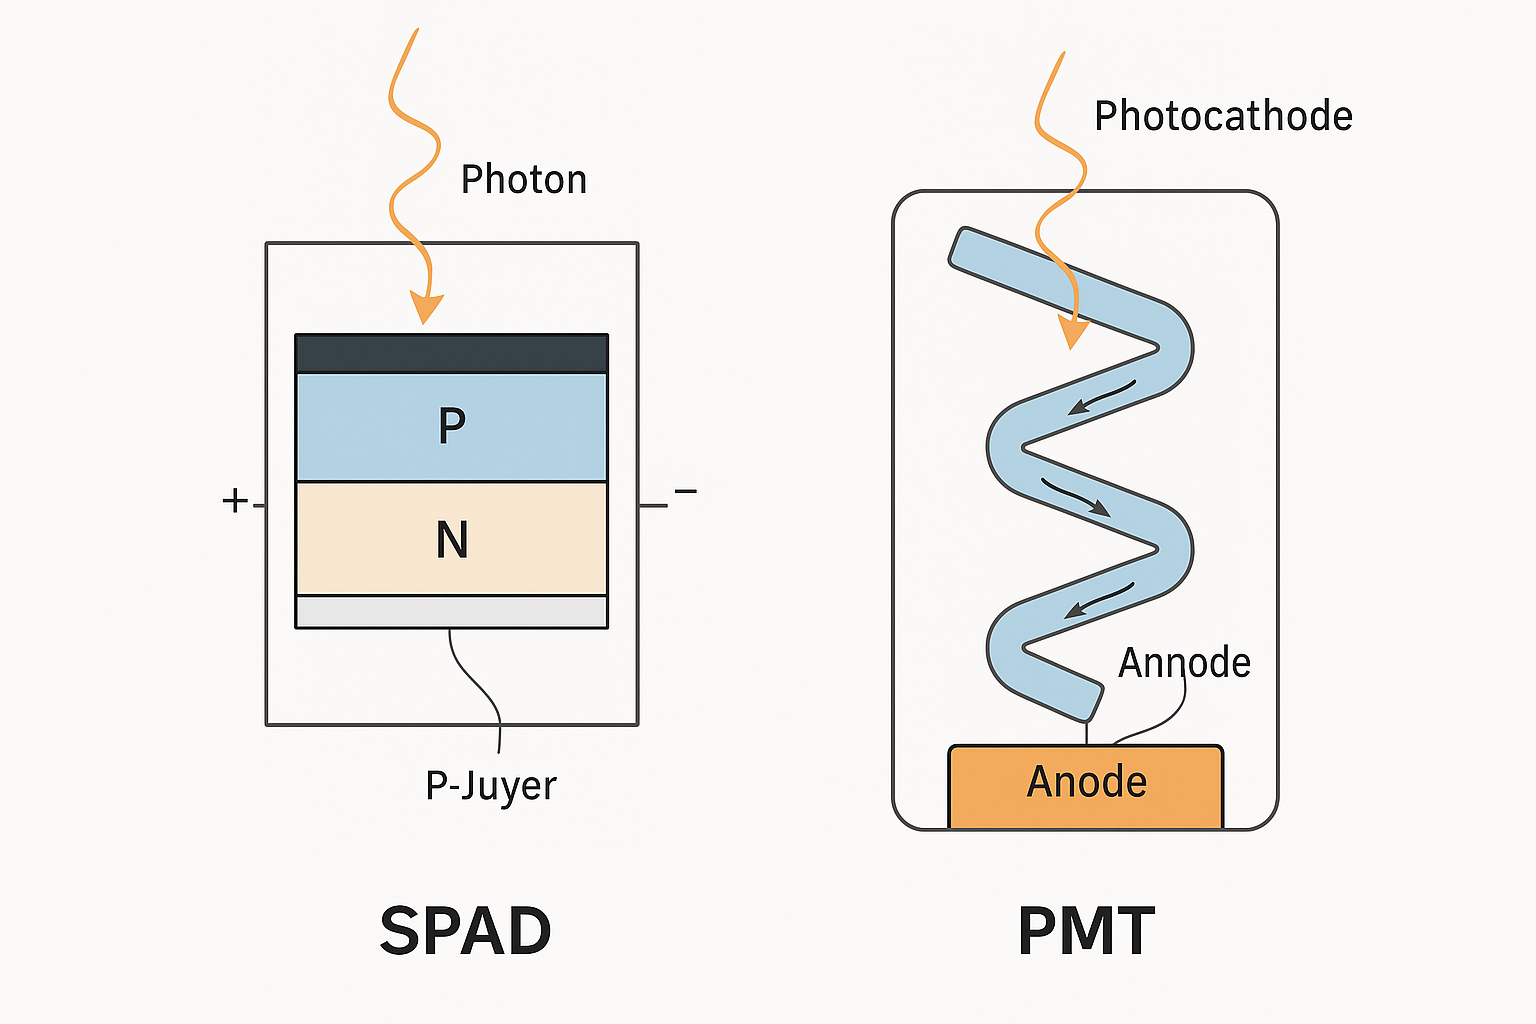
\includegraphics[width=0.9\textwidth]{bilder/SPAD-PMT.png}
	\caption{Schematic comparison of a SPAD (Single-Photon Avalanche Diode, left) and a PMT (Photomultiplier Tube, right). }
	\label{fig:spad_pmt}
\end{figure}
\begin{tcolorbox}[hinweisbox, title=Didactic Comparison: SPAD vs. PMT]
	\label{box:vergleich SPAD}
	\small
	\begin{tabular}{p{0.48\textwidth} | p{0.48\textwidth}}
		\textbf{Single-Photon Avalanche Diode (SPAD)} & \textbf{Photomultiplier Tube (PMT)} \\
		\hline
		Semiconductor device with a special PN junction\index{PN junction}. & Vacuum tube\index{Vacuum tube} with photocathode and amplification stages. \\
		\hline
		A photon generates an electron–hole pair\index{Electron–hole pair} in the depletion region\index{Depletion region}. & A photon knocks an electron out of the photocathode. \\
		\hline
		The electron triggers an avalanche breakdown\index{Avalanche breakdown} – producing an electrical pulse. & The electron is accelerated and multiplied across multiple dynodes. \\
		\hline
		Very high time resolution\index{Time resolution}, ideal for compact, integrated quantum sensors\index{Quantum sensor}. & High gain, ideal for weak light sources (e.g., scintillators\index{Scintillator}). \\
		\hline
		Operates at room temperature\index{Room temperature}, easily integrated into chips\index{Chip}. & Requires high voltage, sensitive to magnetic fields. \\
		\hline
		Well suited for arrays and imaging systems (SiPM). & Traditionally used in nuclear physics\index{Nuclear physics}, astronomy, PET\index{Positron emission tomography}, etc. \\
	\end{tabular}
\end{tcolorbox}
\begin{tcolorbox}[didaktikbox, title=Concept: Avalanche Breakdown]
	\label{box:avalanche}
	\small
	In an \textbf{avalanche breakdown}, a free electron in the strong electric field\index{Electric field} of a semiconductor generates additional electrons through impact ionization\index{Impact ionization}. This process multiplies like an avalanche and produces a measurable current pulse\index{Current pulse} – enabling the detection of a single photon.
\end{tcolorbox}
\vspace{1em}
\begin{tcolorbox}[didaktikbox, title=Concept: Scintillator]
	\label{box:szintillator}
	\small
	A \textbf{scintillator} is a material\index{Material} that emits light\index{Light} when struck by ionizing particles\index{Ionizing particle}. This so-called \emph{scintillation light}\index{Scintillation light} can be registered by photon detectors such as PMTs or SiPMs, enabling the indirect measurement of radiation\index{Radiation}.
\end{tcolorbox}

\subsubsection{Single-Photon Counting and Quantum Efficiency\index{Single-photon counting}\index{Quantum efficiency}}

The ability to \textbf{detect individual photons}\index{Photon} is a milestone in quantum technology\index{Quantum technology}. Here, not only “counting” is important, but also the \textbf{quantum efficiency}\index{Quantum efficiency}, i.e., the fraction of incident photons that actually produce a measurable signal.
\vspace{1em}
\begin{tcolorbox}[physikbox, title=Physical Terms]
	\label{box:begriffe}
	\small
	\begin{itemize}
		\item \textbf{Single-photon counting:} Detection methods in which each registered signal can be assigned to a single photon.
		\item \textbf{Quantum efficiency (QE):} Ratio of registered to incident photons, typically wavelength-dependent\index{Wavelength}.
	\end{itemize}
\end{tcolorbox}

Technically, SPADs\index{SPAD} or superconducting nanodetectors\index{Superconducting nanodetector} are most commonly used. The latter achieve quantum efficiencies close to 100\%, but must be operated cryogenically\index{Cryogenics}.
\newpage
\noindent
\subsubsection*{How Does Single-Photon Counting Work?}
\phantomsection
In single-photon counting, each individual photon pulse is registered as a discrete event. The detector (e.g., a SPAD) generates an electrical pulse when a photon arrives – typically a short voltage or current spike. These pulses are electronically processed:

\begin{itemize}
	\item Each pulse corresponds to one detected photon.
	\item A counter\index{Counter} sums these pulses over defined time intervals.
	\item The result is a photon count per interval – e.g., “125 photons in 1 ms.”
\end{itemize}

For this to work reliably, the pulses must:
\begin{itemize}
	\item exceed a clear \textbf{threshold} (threshold detection\index{Threshold detection}),
	\item be temporally well separated (observe dead time\index{Dead time}),
	\item and not be confused with \textbf{thermal noise}\index{Thermal noise} or dark current\index{Dark current}.
\end{itemize}
\vspace{1em}
\begin{tcolorbox}[didaktikbox, title=What Counts as a Photon? ]
	\label{box:photonenzaehlung}
	\small
	Not every registered pulse originates from a photon. Detectors also produce \emph{dark counts}\index{Dark count} (false signals without incoming light). High-quality single-photon detectors, however, achieve dark count rates below 100 pulses per second and quantum efficiencies of 50–90\%.
\end{tcolorbox}

\subsubsection{Applications in Industry and Fundamental Physics\index{Applications!Photon detection}}

The applications of photonic sensing are diverse:

\begin{itemize}
	\item \textbf{Fundamental physics\index{Fundamental physics}:} Detection of individual photons in quantum optics\index{Quantum optics} experiments (e.g., antibunching\index{Antibunching}, HOM effect\index{Hong–Ou–Mandel effect}), particle detection in high-energy physics\index{High-energy physics}, astronomical observations\index{Astronomy} (e.g., Hubble\index{Hubble Space Telescope}, JWST\index{James Webb Space Telescope}).
	\item \textbf{Industrial applications\index{Industry}:} Quality control\index{Quality control}, laser scanners\index{Laser scanner}, light curtains\index{Light curtain}, position sensors\index{Position sensor}, photon spectroscopy\index{Photon spectroscopy}.
	\item \textbf{Medicine and life sciences\index{Medicine}:} Fluorescence microscopy\index{Fluorescence microscopy}, PET scanners\index{Positron emission tomography}, optical tomography\index{Optical tomography}.
\end{itemize}

\begin{tcolorbox}[hinweisbox, title=Note on the Importance of Detection Technology]
	\label{box:detektionstechnologie}
	The continuous improvement of photon detection is a prerequisite for progress in quantum communication\index{Quantum communication}, medical imaging\index{Medical imaging}, and fundamental research\index{Fundamental research}. Many developments in quantum technology directly depend on the ability to detect photons precisely and with minimal loss.
\end{tcolorbox}
\subsection{Photons in Medical Imaging\index{Photons in medical imaging}}

Photons play a central role in many imaging techniques of modern medicine. Their range of use extends from high-energy X-rays\index{X-rays} to gentle visible laser light\index{Laser light} in optical diagnostics\index{Optical diagnostics}. Different physical processes – absorption\index{Absorption}, scattering\index{Scattering}, fluorescence\index{Fluorescence}, or emission\index{Emission} – are employed to make contrast in tissue visible or to identify pathological structures.

\subsubsection{X-ray, CT, and PET}

\textbf{X-rays}\index{X-rays} are based on high-energy photons, which generate an image through absorption and attenuation when passing through the body. Denser tissue (e.g., bone) absorbs more photons and appears brighter on the detector.

\textbf{Computed tomography (CT)}\index{Computed tomography (CT)} extends this technique by reconstructing a 3D image from many X-ray projections. Rotating X-ray sources and detector arrays are used for this purpose.

\textbf{Positron emission tomography (PET)}\index{Positron emission tomography (PET)} uses a different mechanism: Radiopharmaceuticals\index{Radiopharmaceutical} emit positrons\index{Positron}, which annihilate with electrons\index{Electron} – producing two photons with an energy of \SI{511}{keV} emitted in opposite directions. These are registered by ring detectors, and from the coincidence of detection, the origin is reconstructed.
\vspace{1em}
\begin{tcolorbox}[physikbox, title=Photons in PET]
	\label{box:PET}
	\small
	In PET, two gamma photons of \SI{511}{keV} are created in the annihilation of an electron and a positron. These photons leave the body almost unhindered and allow for precise localization of metabolism – e.g., in tumors.
\end{tcolorbox}
\begin{figure}[H]
	\centering
	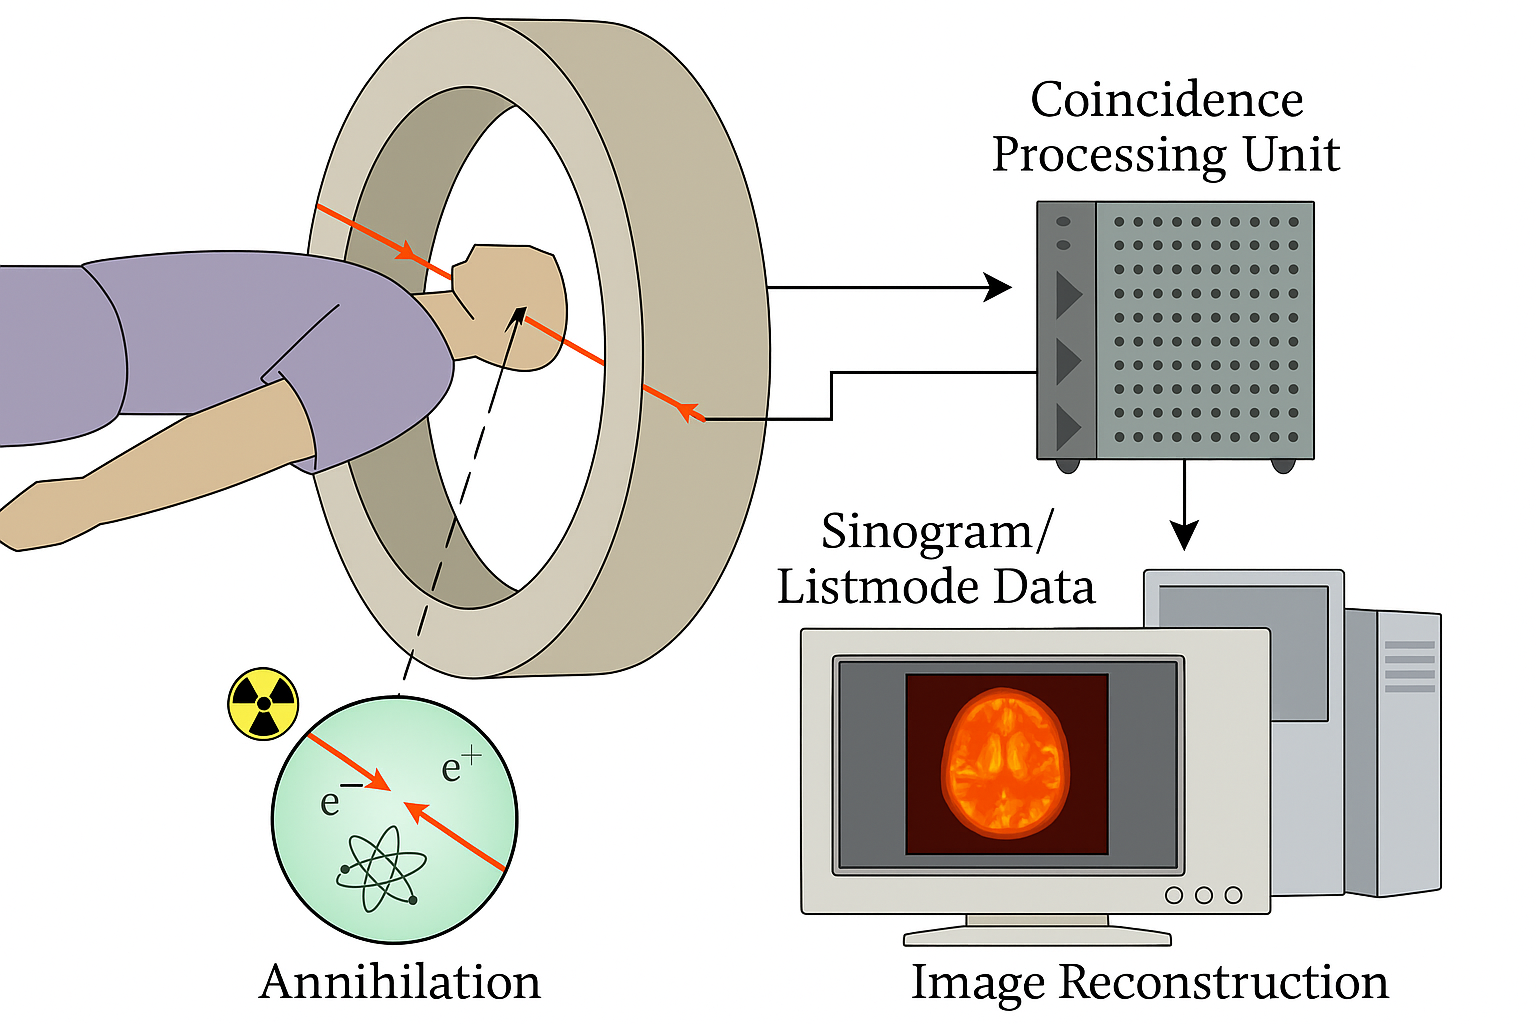
\includegraphics[width=0.85\textwidth]{bilder/petscan.png}
	\caption{Principle of positron emission tomography (PET): A radiopharmaceutical administered into the body emits a positron, which annihilates with an electron. Two gamma photons of \SI{511}{keV} each are emitted in opposite directions and registered by detectors in the PET ring. From the coincidence of signals, the point of origin is reconstructed.}
	\label{fig:pet_prinzip}
\end{figure}
\begin{tcolorbox}[didaktikbox, title=Concept: Annihilation]
	\label{box:annihilation}
	\small
	In \textbf{annihilation}, a particle and its antiparticle collide and annihilate each other. Their mass is fully converted into energy – usually in the form of photons. In PET, annihilation of an electron with a positron produces a photon pair of \SI{511}{keV} each.
\end{tcolorbox}
\vspace{1em}
\begin{tcolorbox}[didaktikbox, title=Concept: Radiopharmaceutical]
	\label{box:radiopharmakon}
	\small
	A \textbf{radiopharmaceutical} is a radioactively labeled compound administered specifically into the body. In PET, for example, [\textsuperscript{18}F]FDG is used – a sugar-like substance that accumulates in metabolically active tissues (such as tumors). The positrons produced there provide the image signal through annihilation.
\end{tcolorbox}

\subsubsection{Optical Tomography and Fluorescence Imaging}

In contrast to ionizing radiation, these techniques rely on visible or near-infrared light.

\textbf{Diffuse optical tomography (DOT)}\index{Diffuse optical tomography (DOT)} uses light sources and detectors on the skin surface. Photons penetrate the tissue, are scattered and absorbed. From the light distribution, the optical properties inside can be reconstructed.

\textbf{Fluorescence imaging}\index{Fluorescence imaging} employs substances (fluorophores\index{Fluorophore}) that are excited by light and re-emit at a different wavelength. This method allows, for example, the visualization of molecular processes or tumor markers.
\vspace{1em}
\begin{tcolorbox}[didaktikbox, title=Advantage of Optical Methods]
	\label{box:optisches Verfahren}
	\small
	Optical methods are non-invasive, free of ionizing radiation, and are particularly suitable for surface and functional imaging – e.g., in infants, neurodiagnostics, or molecular imaging.
\end{tcolorbox}

\subsubsection{Lasers in Surgery and Diagnostics}

Lasers\index{Laser} are used both for \textbf{imaging} and for \textbf{tissue interaction}:

\begin{itemize}
	\item \textbf{Diagnostic:} Confocal laser scanning microscopy\index{Confocal laser scanning microscopy}, optical coherence tomography (OCT)\index{Optical coherence tomography (OCT)}, spectroscopy\index{Spectroscopy}.
	\item \textbf{Surgical:} Tissue cutting, coagulation, ablation – depending on wavelength, pulse duration, and power.
\end{itemize}

Laser surgery\index{Laser surgery} exploits the precise focusing of photons for targeted tissue treatment without mechanical stress. Typical applications are:

\begin{itemize}
	\item Ophthalmology\index{Ophthalmology} (e.g., LASIK\index{LASIK}),
	\item Dermatology\index{Dermatology} (e.g., tattoo removal\index{Tattoo removal}),
	\item Tumor surgery\index{Tumor surgery} (precise cuts with minimal blood loss).
\end{itemize}

\begin{tcolorbox}[hinweisbox, title=Laser Parameters]
	\label{box:laserparameter}
	\small
	The effect of a laser strongly depends on its wavelength, pulse duration, energy, and focusing. Short pulses with high power allow precise cuts without damaging the surrounding tissue.
\end{tcolorbox}
\newpage
\noindent
\begin{figure}[H]
	\centering
	\includegraphics[width=0.85\textwidth]{bilder/oct.png}
	\caption{Schematic representation of optical coherence tomography (OCT): Light from a broadband source is split by a beam splitter. One part hits a movable reference mirror (reference arm), the other the tissue to be examined (sample). The reflected light portions interfere, and from the interference patterns the depth profile is reconstructed. The result is a high-resolution image, e.g., of the retina.}
	\label{fig:oct_prinzip}
\end{figure}

\begin{tcolorbox}[didaktikbox, title=Didactic Explanation: Interference in OCT]
	\label{box:interferenz_oct}
	\small
	\textbf{Interference} occurs when two light waves overlap – depending on the phase, they either reinforce or cancel each other. In OCT, this property is used to determine the position of reflecting structures in tissue with high precision.
	
	Only when the optical path lengths in the \emph{sample arm} and the \emph{reference arm} are nearly equal does an interference signal occur. From the measured intensity as a function of the reference arm position, an \textbf{A-scan} – a depth profile along a line in the tissue – is obtained.
	
	By laterally shifting the measurement beam, many A-scans next to each other are recorded, which together form a \textbf{B-scan} (2D cross-section). This produces a detailed image of the examined tissue – e.g., of the retina.
\end{tcolorbox}

\subsection{Photons in Communication}
\index{Photons in communication}
\index{Data transmission}
\index{Quantum communication}

Photons form the backbone of modern data transmission – both in classical fiber optic networks and in future quantum-based systems. The low-loss propagation of light in optical media, combined with high bandwidth and low latency, makes photonic communication technology a decisive factor in global information infrastructure.

\subsubsection{Optical Fiber and Optical Networks}
\index{Optical fiber}
\index{Optical networks}
\index{Total internal reflection}
\index{Wavelength division multiplexing}
\index{DWDM}
\index{EDFA}

\textbf{Optical fibers} guide light by total internal reflection in a thin quartz core. Photons can thus be transmitted over distances of several hundred kilometers with minimal attenuation.

Advantages:
\begin{itemize}
	\item extremely high data rates (terabits/s),
	\item immunity to electromagnetic interference,
	\item low attenuation (e.g., \SI{0.2}{dB/km} at \SI{1550}{nm}).
\end{itemize}

\textbf{Optical networks} use wavelength division multiplexing (DWDM), amplifiers (EDFAs), and modulated laser systems to transmit large amounts of data in parallel and efficiently – from backbone networks to fiber-to-the-home connections.
\vspace{1em}
\begin{tcolorbox}[physikbox, title=Total Internal Reflection in Optical Fibers]
	\label{box:glasfaser}
	\small
	Light guidance in an optical fiber is based on total internal reflection at the interface between the higher-refractive-index core and the cladding. The critical angle determines whether the light remains “trapped” inside the core.
\end{tcolorbox}
\newpage
\noindent
\begin{figure}[H]
	\centering
	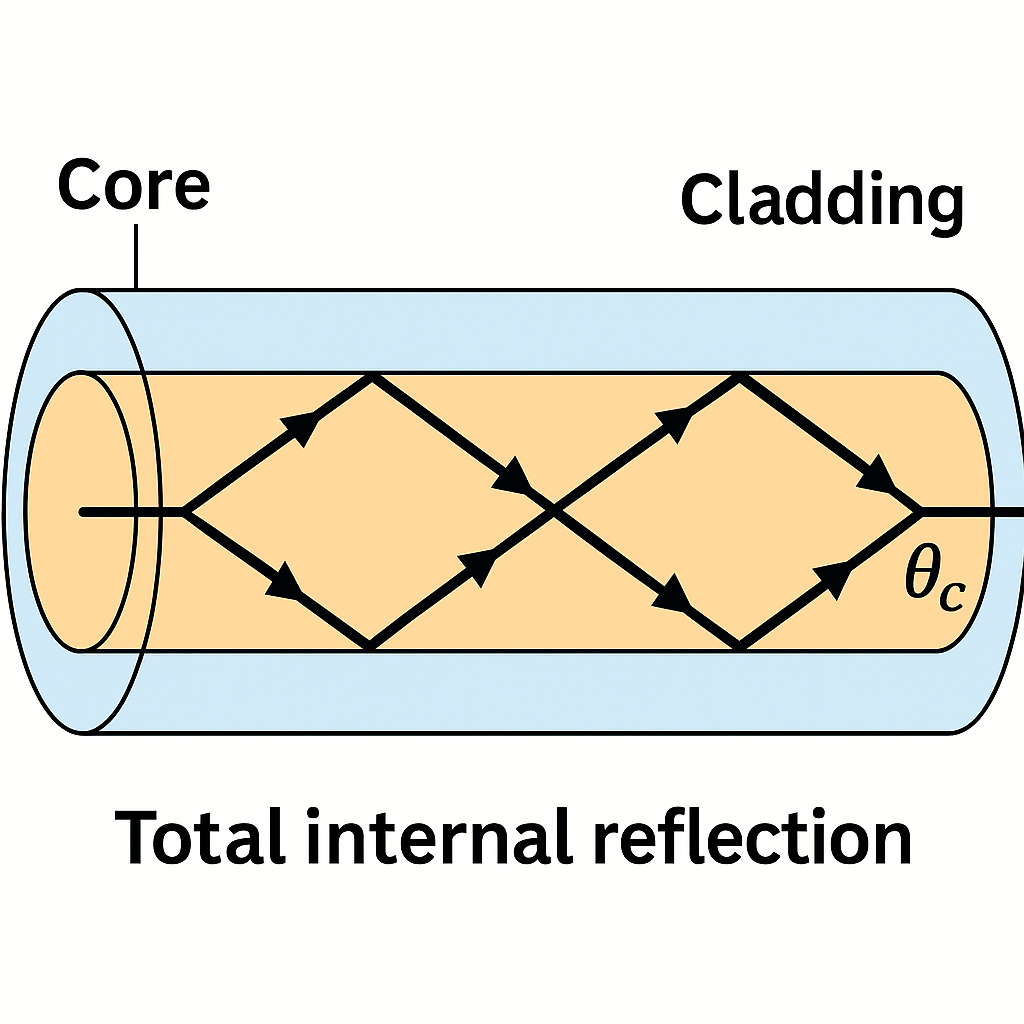
\includegraphics[width=0.8\textwidth]{bilder/glasfaser.png}
	\caption{Schematic illustration of total internal reflection in an optical fiber: Light (photons) is guided in the higher-index core and fully reflected at the interface with the cladding. This keeps the light “trapped” in the core even over long distances.}
	\label{fig:totalreflexion}
\end{figure}
\subsubsection{Quantum Communication and QKD}\index{Quantum communication}\index{QKD}\index{Photons!Quantum communication}\index{Polarization!Photons}\index{Entanglement!Photons}

\textbf{Quantum communication} exploits quantum states of photons – such as polarization or entanglement – to transmit information in a way that is absolutely secure against eavesdropping.

\textbf{QKD (Quantum Key Distribution)} is a practical application: Two parties (Alice and Bob) exchange a secret key. Any eavesdropping attempt (Eve) inevitably alters the quantum state of the photons and can thus be detected.
\newpage
\noindent
\begin{tcolorbox}[didaktikbox, title=What Makes QKD Secure?] \index{QKD!Security}
	\label{box:qkd}
	\small
	The security relies on two quantum-physical principles:
	\begin{itemize}
		\item \textbf{No-cloning theorem:} Unknown quantum states cannot be perfectly copied.
		\item \textbf{Measurement disturbance:} Any measurement affects the state – an eavesdropping attempt measurably disturbs the system.
	\end{itemize}
\end{tcolorbox}

\textbf{BB84} is the first and best-known QKD protocol. It uses random polarizations and basis changes to generate a key, which is then verified over a classical channel.

\vspace{1em}
\begin{tcolorbox}[didaktikbox, title={How Does QKD Work (e.g., BB84)?}] \index{QKD!BB84}\index{Quantum communication!BB84}
	\label{box:wie funktioniert QKD}
	\small
	In the BB84 protocol, Alice sends single photons whose polarization is randomly chosen – e.g., horizontal ($\rightarrow$), vertical ($\uparrow$), diagonal ($\searrow$), or anti-diagonal ($\nwarrow$). Bob also measures in random bases.
	
	Only when sender and receiver bases match does a valid bit result. After the exchange, Alice and Bob (publicly) compare the bases used and keep only the matching ones. From these bits, the key is generated.
	
	If a photon is intercepted, its polarization changes – allowing Alice and Bob to detect disturbances in the key and reveal eavesdropping attempts.
\end{tcolorbox}

\subsubsection{Photonic Chips and Future Systems}\index{Photonic chips}\index{Silicon photonics}\index{Photons!Photonic chips}\index{Data processing!Photonic}\index{Logic systems!Photonic}

With the advent of \textbf{photonic chips}, light signals are no longer guided solely through optical fibers but directly through integrated optical circuits. These enable:

\begin{itemize}
	\item compact, energy-efficient data processing,
	\item light-based logic and modulation systems,
	\item new concepts for neural networks and AI accelerators.
\end{itemize}

Photonic chips combine lasers, modulators, waveguides, and detectors on a single substrate – often silicon photonics.
\newpage
\noindent
\begin{tcolorbox}[hinweisbox, title=Future of Photonic Communication] \index{Photon-based communication}
	\label{box:Zukunft Kommunikation}
	\small
	Photon-based communication is not only faster than classical electronics – it will become a prerequisite for secure quantum networks, light-based processors, and global, tap-proof communication.
\end{tcolorbox}

\subsection{Photons in Astronomical Observation}\index{Astronomy!Photons}\index{Photons!Astronomy}\index{Photons!Astronomical observation}

The observation of photons from space is the foundation of modern astronomy. Since photons – unlike, for example, gravitational waves or neutrinos – are comparatively easy to detect, they provide most of our information about the universe. Whether visible light, radio waves, or high-energy gamma rays – every photon reaching Earth carries a message from space and time.

\subsubsection{Detection of Photons from Space}\index{Detection!Photons}\index{Photons!Detection!Astronomical}

Telescopes and detectors on Earth and in space measure photons across various wavelength ranges:

\begin{itemize}
	\item \textbf{Optical range:} CCDs (charge-coupled devices), CMOS sensors
	\item \textbf{Infrared and radio:} Bolometers, radio telescopes
	\item \textbf{X-rays and gamma rays:} Space telescopes with scintillators and semiconductor detectors
\end{itemize}

The analysis of these photons provides information about temperature, motion (Doppler shift), composition, and distance of cosmic objects.

\vspace{1em}
\begin{tcolorbox}[physikbox, title=Why Don’t All Photons Reach Earth?] \index{Earth’s atmosphere!Photon absorption}\index{Photons!Earth’s atmosphere}
	\label{box:photonen auf erde}
	\small
	The Earth’s atmosphere is opaque to many wavelength ranges – especially UV, X-rays, and gamma rays. Therefore, corresponding telescopes must be positioned outside the atmosphere – e.g., in Earth orbit.
\end{tcolorbox}
\newpage
\noindent
\subsubsection{Adaptive Optics, Spectroscopy, and Telescopes}
\index{Adaptive optics}
\index{Spectroscopy}
\index{Telescopes}
\index{Interferometry}

\textbf{Telescopes} collect photons\index{Photon} and focus them onto detectors. Modern large telescopes (e.g., the VLT\index{Very Large Telescope (VLT)} or ELT\index{Extremely Large Telescope (ELT)}) use adaptive optics to improve image quality:

- \textbf{Adaptive optics} compensates for atmospheric distortions in real time using deformable mirrors.
- \textbf{Spectroscopy} disperses light into its wavelengths and allows the analysis of chemical composition, temperature, and motion of celestial bodies.
- \textbf{Interferometry} combines several telescopes into a virtual giant telescope with extremely high angular resolution.
\begin{figure}[H]
	\centering
	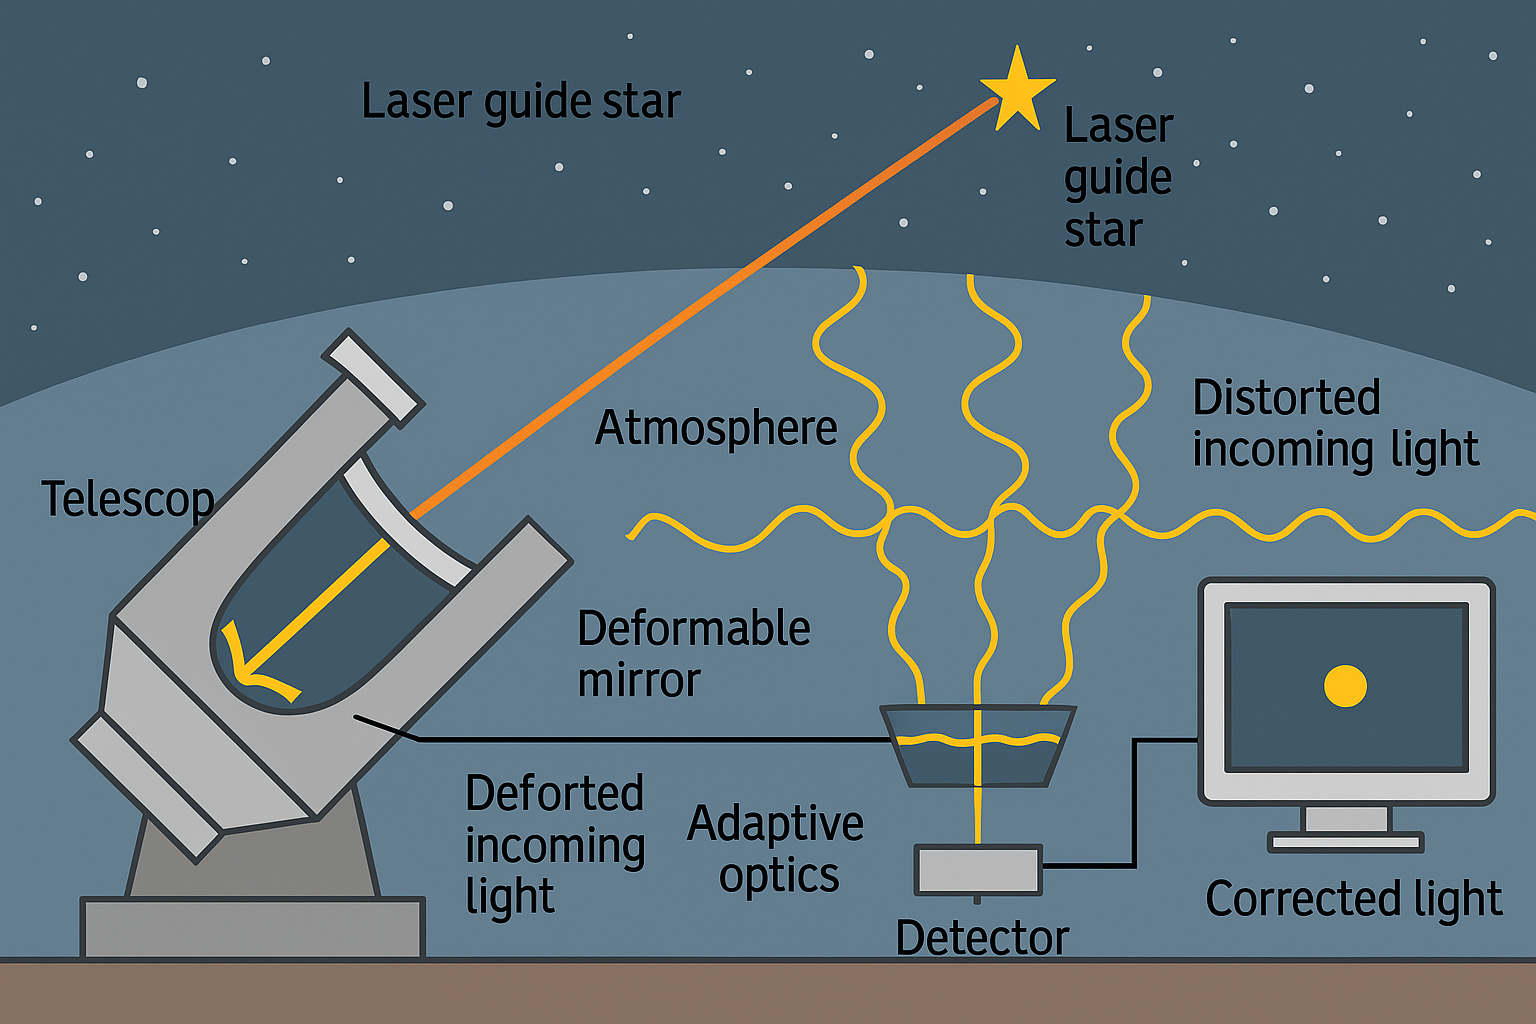
\includegraphics[width=0.9\textwidth]{bilder/Teleskop.png}
	\caption{Schematic illustration of a telescope with adaptive optics. A wavefront sensor analyzes distortions caused by the atmosphere. A deformable mirror surface corrects these in real time, producing a sharp image.}
	\label{fig:adaptive_optik}
\end{figure}

\begin{tcolorbox}[didaktikbox, title=What Does a Spectrum Show?]
	\label{box:was zeigt spektrum}
	\small
	A \textbf{spectrum}\index{Spectrum} is the distribution of photon intensity as a function of wavelength. Typical features include:
	\begin{itemize}
		\item \textbf{Emission lines}\index{Emission lines} $\rightarrow$ hot, radiating gases,
		\item \textbf{Absorption lines}\index{Absorption lines} $\rightarrow$ cold gases in front of hot sources,
		\item \textbf{Redshift}\index{Redshift} $\rightarrow$ motion of the object away from the observer.
	\end{itemize}
\end{tcolorbox}
\begin{figure}[H]
	\centering
	
\includegraphics[width=0.9\textwidth]{bilder/emissionslinien.png}
	\caption{Emission spectrum of glowing hydrogen gas.}
	\label{fig:emission_hydrogen}
\end{figure}

\begin{tcolorbox}[physikbox, title=Spectral Lines and Redshift]
	\label{box:spektrallinien}
	\small
	\begin{itemize}
		\item \textbf{Emission lines} arise when atoms emit specific photons. These lines are bright and characteristic of the respective element\index{Element spectrum}.
		\item \textbf{Absorption lines} occur when photons of certain frequencies are absorbed by a gas through which the light passes – they then appear missing in the spectrum.
		\item \textbf{Redshift:} When a light source moves away, all lines shift to longer wavelengths – toward red. This is used to measure cosmic motion\index{Cosmic expansion}.
	\end{itemize}
\end{tcolorbox}

\subsubsection{Photons in Gravitational Wave Astronomy}
\index{Gravitational wave astronomy}
\index{Gravitational waves}
\index{Photon}
\index{Interferometer}
\index{LIGO}
\index{Virgo}

Gravitational waves are fundamental distortions of spacetime\index{Spacetime} – triggered by accelerated masses, such as the merger of black holes\index{Black hole}. They are not electromagnetic waves and are not made of photons. Nevertheless, it is precisely photons that enable their detection: as precise probes in highly sensitive interferometers.

\vspace{0.5em}
\textbf{LIGO, Virgo, and other gravitational wave detectors} use kilometer-scale laser interferometers to measure minute changes in spacetime. Laser beams (consisting of coherent photons) are sent into two perpendicular arms, reflected by mirrors, and recombined at the output. A passing gravitational wave slightly changes the arm lengths – and thus the interference pattern.

\vspace{1em}
\begin{tcolorbox}[physikbox, title=Photons as a Tool for Measuring Spacetime Curvature]
	\label{box:messwerkzeug}
	\small
	Laser interferometers such as LIGO use photons to detect differences in arm length as small as \SI{1e-19}{m} – about a thousand times smaller than a proton\index{Proton}. The time difference a photon needs to traverse the two arms changes measurably due to a passing gravitational wave.
\end{tcolorbox}

This technique relies on the interference\index{Interference} of coherent light waves. When the two beams are recombined after traveling through the arms, constructive or destructive interference occurs depending on the phase shift. Even the smallest changes in optical path length affect this pattern. In this way, even minute curvatures of spacetime can be detected.

\vspace{0.5em}
Thanks to this photon-based precision measurement, events such as black hole mergers, neutron star collisions\index{Neutron star}, or traces of the cosmic gravitational background\index{Cosmic gravitational background} have been experimentally confirmed. Photons thus make visible what would otherwise lie beyond direct observation – further evidence of their central role in modern physics.
\newpage
\noindent
\vspace{1em}
\begin{tcolorbox}[didaktikbox, title=How Does an Interferometer Work? \label{box:interferometer}]
	\small
	An interferometer uses the principle of superposition (interference) of light waves to make the smallest length differences visible. 
	
	\begin{itemize}
		\item A laser beam\index{Laser} is split into two partial beams using a beam splitter.
		\item These travel along two perpendicular arms to mirrors, are reflected, and recombined.
		\item If the optical path lengths of the two arms are exactly equal, the waves cancel each other partly or completely – the interference pattern is constant.
		\item If one arm length changes slightly (e.g., due to a gravitational wave), the phase of one wave shifts, and the interference pattern measurably changes.
	\end{itemize}
	
	Thus, even length changes smaller than an atom’s diameter can be detected by analyzing the light intensity at the detector. Light serves as a precise “measuring stick” in space.
\end{tcolorbox}

\vspace{1em}
\begin{tcolorbox}[didaktikbox, title=Why Are Photons So Precisely Measurable? \label{box:photonen_genau}]
	\small
	Photons are ideal measurement tools – for several reasons:
	
	\begin{itemize}
		\item \textbf{High coherence:} Laser light consists of coherent photons – i.e., waves with exactly the same frequency and stable phase. This enables extremely sensitive interference effects.
		\item \textbf{Low interaction:} Photons hardly interact with matter. This allows long propagation paths without disturbance or deflection.
		\item \textbf{Quantum nature:} Single photons are discrete quantum objects\index{Quantum nature}. Their detection produces clear, countable signals – ideal for precise time or position measurements.
		\item \textbf{Speed of light as a constant:} The velocity of photons in a vacuum is constant\index{Speed of light}. This makes them natural “standards” for time and length.
	\end{itemize}
	
	These properties make photons indispensable in modern metrology – from interferometers to quantum sensors\index{Quantum sensor} to optical atomic clocks\index{Optical atomic clock}.
\end{tcolorbox}

\subsubsection{Conclusion}

Photons are not only central objects of modern physics but also indispensable tools in science, engineering, medicine, and communication. This chapter has shown how diverse and precise photons can be controlled, generated, and detected:

\begin{itemize}
	\item In \textbf{laser technology}\index{Laser technology}, stimulated emission and coherent light amplification enable applications ranging from materials processing to quantum optics\index{Quantum optics}.
	\item \textbf{Photon detectors}\index{Photon detector} such as SPADs\index{SPAD} or PMTs\index{Photomultiplier (PMT)} allow single-photon counting with high quantum efficiency\index{Quantum efficiency} – a foundation for quantum technologies\index{Quantum technology} and precise imaging.
	\item In \textbf{medical diagnostics}\index{Medical diagnostics}, photons are used for imaging with high spatial resolution and minimal exposure – from X-rays\index{X-rays} to fluorescence microscopy\index{Fluorescence microscopy}.
	\item \textbf{Optical communication}\index{Optical communication} uses photons for fast, low-loss, and secure data transmission – in fibers\index{Optical fiber} as well as in quantum communication systems\index{Quantum communication}.
	\item In \textbf{astronomical observation}\index{Astronomy}, photons provide crucial information about the structure, motion, and composition of the universe – up to the detection of gravitational waves through interferometric measurement.
\end{itemize}

The ability to deliberately generate, guide, and measure single photons marks a technological turning point: From classical applications to quantum information technology\index{Quantum information technology}, the photon opens new horizons – in research, industry, and society.

	\chapter{Photons and the Future of Physics}
\setcounter{section}{7}
\setcounter{subsection}{0}
\setcounter{subsubsection}{1}
\setcounter{secnumdepth}{3}
% Box styles
\tcbset{physikbox/.style={colback=blue!5!white, colframe=blue!75!black, fonttitle=\bfseries}}
\tcbset{mathebox/.style={colback=green!5!white, colframe=green!50!black, fonttitle=\bfseries}}
\tcbset{didaktikbox/.style={colback=yellow!5!white, colframe=yellow!50!black, fonttitle=\bfseries}}
\tcbset{hypobox/.style={colback=orange!5!white, colframe=orange!75!black, fonttitle=\bfseries}}
\tcbset{hinweisbox/.style={colback=gray!10!white, colframe=black!40!black, fonttitle=\bfseries}}

\subsection{Introduction}
\index{Photon}
\index{Photonics}
\index{Communication}
\index{Metrology}
\index{Data processing}
\index{Photonic computer}
\index{Quantum communication network}
\index{Graviton}
\index{Dark energy}
\index{Standard Model}

Photons not only shape today’s technology but also open doors to entirely new areas of research.  
While they are already indispensable in communication, metrology, and data processing, we are also at the beginning of an era in which photons take on central roles in photonic computers, quantum communication networks, and the most precise experiments in fundamental physics.  
This chapter spans the arc from current developments in photonics to forward-looking applications and the great open questions of physics — from the search for the hypothetical graviton, to the puzzle of dark energy, to possible extensions of the Standard Model.  
The topics presented show how the smallest quantum of light could become the key to the technologies and discoveries of tomorrow.
\newpage
\noindent
\begin{figure}[H]
	\centering
	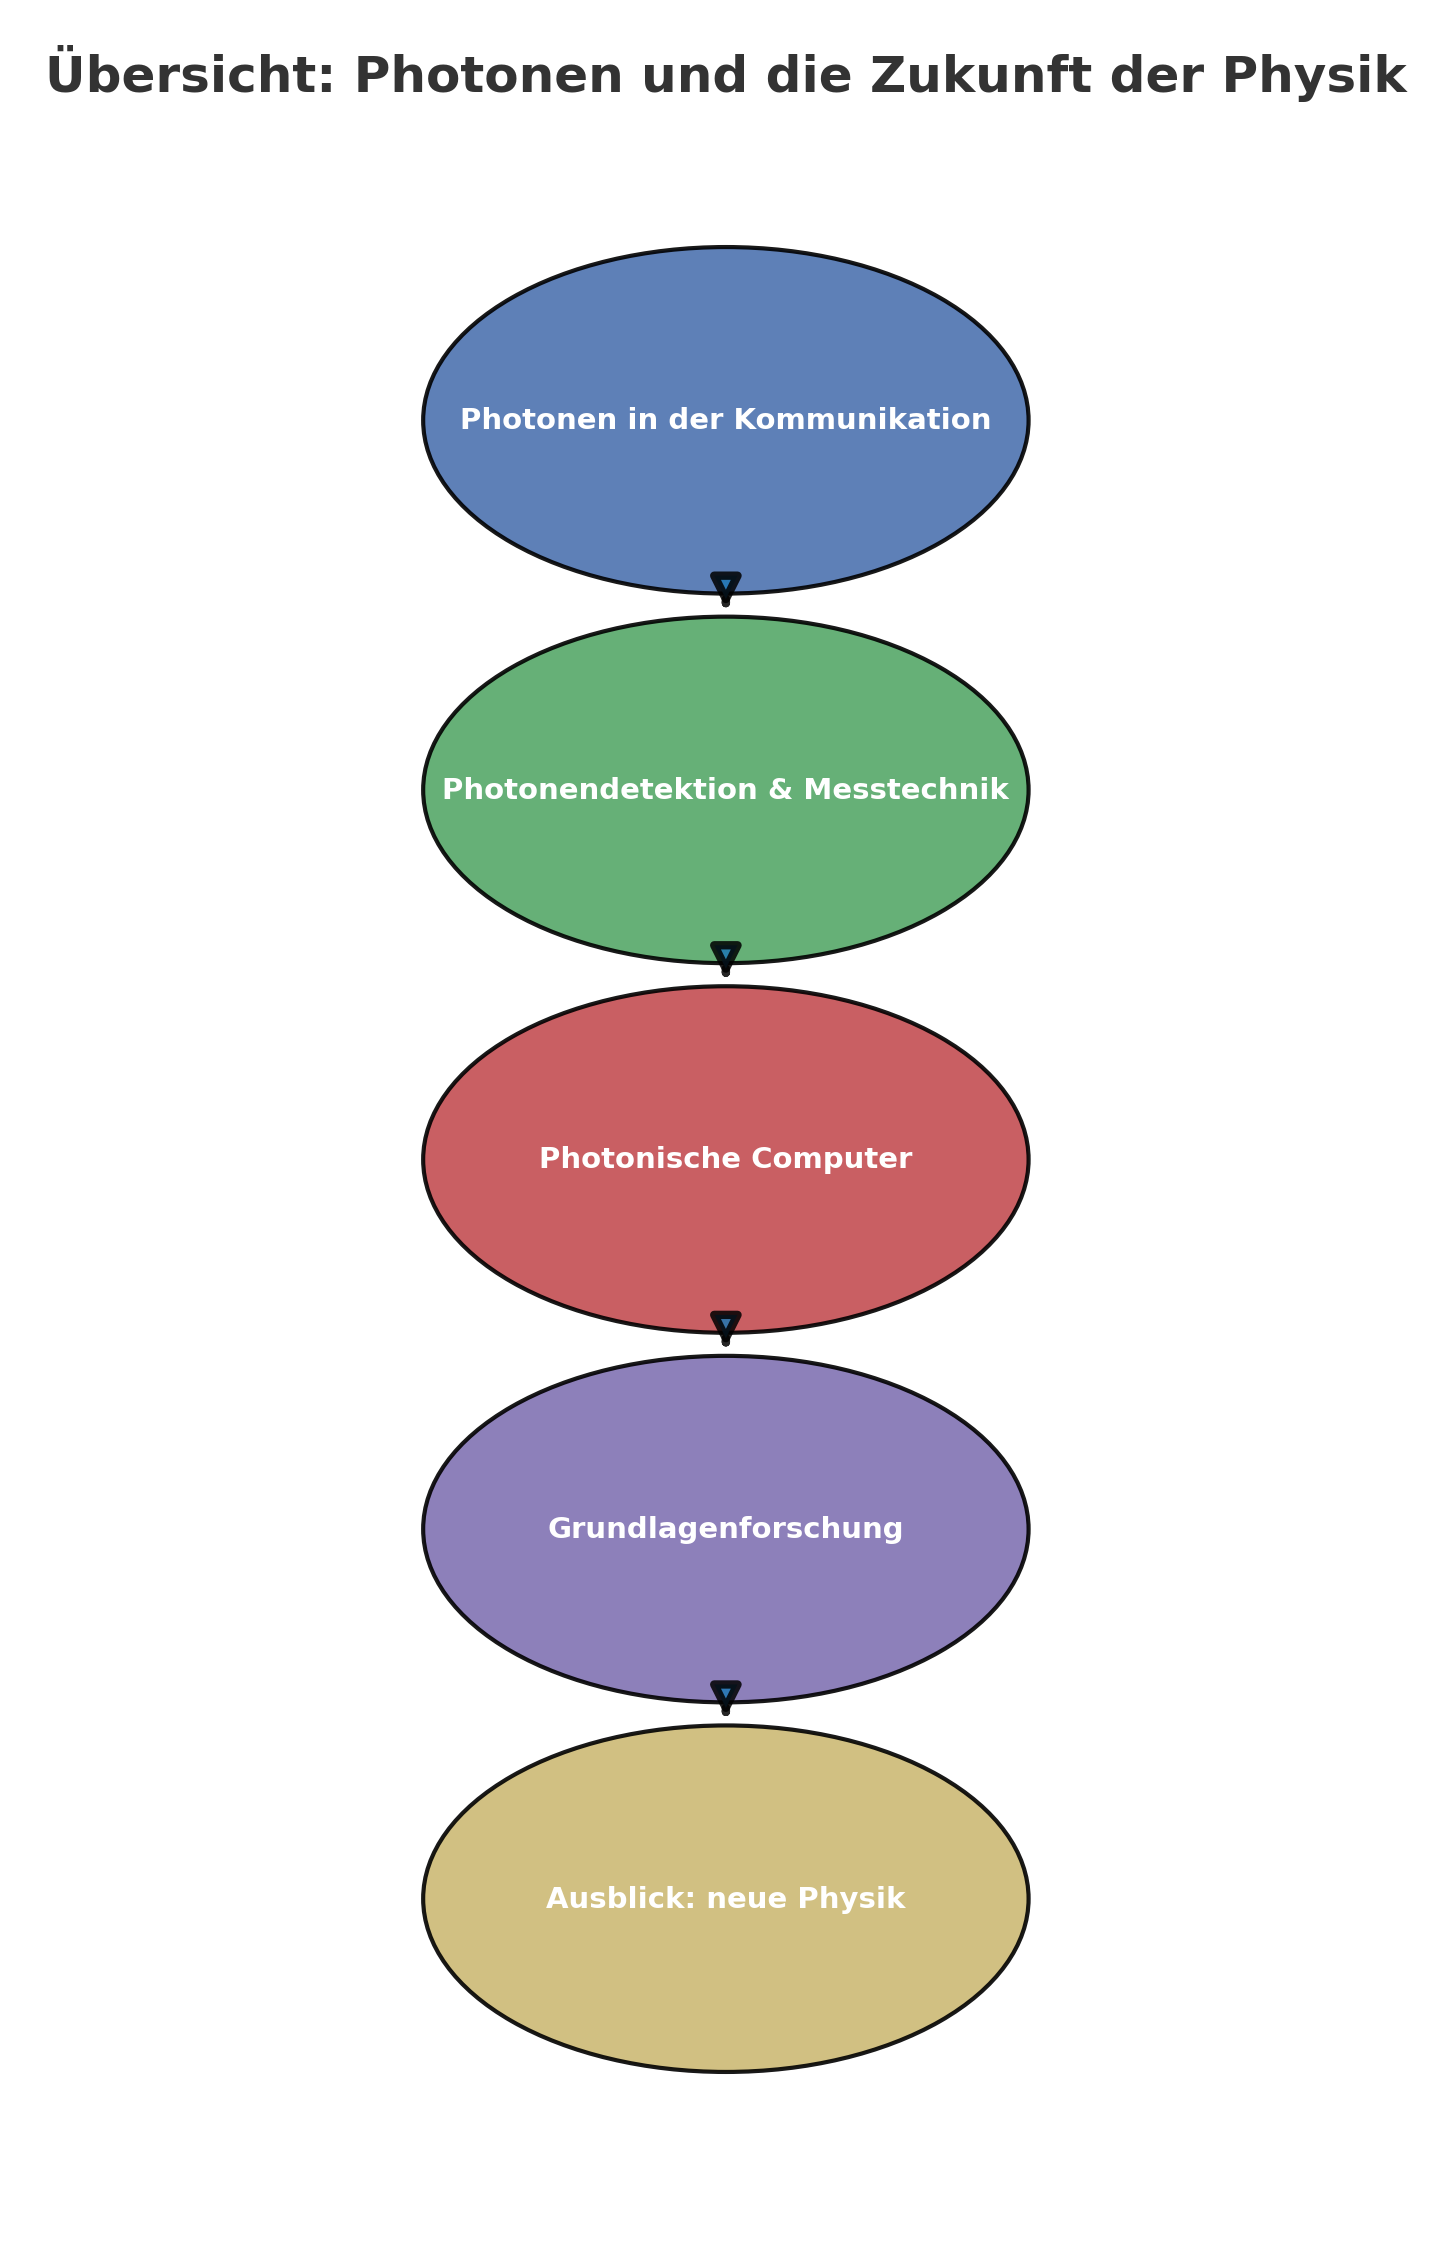
\includegraphics[width=0.75\textwidth]{bilder/kapitel_VII_uebersicht.png}
	\caption[Overview Chapter~VII]{Overview: Photons and the Future of Physics. 
		The graphic shows the main themes of this chapter in a vertical arrangement, 
		from photonic logic to open questions of new physics.}
	\label{fig:kapitel_VII_uebersicht}
\end{figure}

\subsection{Single Photons and Quantum Information}
\index{Single photon}
\index{Quantum information}
\index{Qubit}
\index{Superposition}
\index{Polarization}
\index{Time-bin}
\index{Frequency encoding}

The ability to generate, control, and detect individual photons has taken on a key role in quantum information technology in recent years. Single photons serve as ideal carriers of quantum information: they are robust against disturbances, travel at the speed of light\index{Speed of light}, and can be prepared in well-defined quantum states\index{Quantum state}.

In classical information technology, bits are stored and processed in the form of electrical voltages or magnetic states. In quantum information, by contrast, the smallest unit — the \emph{qubit} — is based on the coherent superposition\index{Superposition} of states. For photons, these states are often realized through polarization directions, time bins, or path information.
\vspace{1em}
\begin{tcolorbox}[physikbox, title=What Makes a Photon an Information Carrier? \label{box:photon_information}]
	\small
	Photons can carry different physical degrees of freedom that are usable as qubits:
	\begin{itemize}
		\item \textbf{Polarization:} Horizontal ($\ket{H}$) and vertical ($\ket{V}$) as basis states.
		\item \textbf{Time bins:} Early and late arrival times as logical states.
		\item \textbf{Path:} Two different optical paths in an interferometer\index{Interferometer}.
		\item \textbf{Frequency:} Different spectral modes for encoded information.
	\end{itemize}
	These degrees of freedom can be precisely controlled and transmitted over long distances without destroying the quantum information.
\end{tcolorbox}

\subsubsection{Generation of Single Photons}
\index{Single-photon source}
\index{Spontaneous parametric down-conversion}
\index{Single atom}
\index{Ion}
\index{Quantum dot}
\index{Nonlinear crystal}
\index{Semiconductor material}

Single-photon sources are central building blocks of quantum optics\index{Quantum optics}. Common methods include:
\begin{itemize}
	\item \emph{Spontaneous parametric down-conversion} (SPDC) in nonlinear crystals.
	\item \emph{Single atoms} or ions in optical traps\index{Optical trap}.
	\item \emph{Quantum dots} in semiconductors.
\end{itemize}
The goal is to generate photons with high purity (low multi-photon probability) and high indistinguishability.
\newpage
\noindent
\vspace{1em}
\begin{tcolorbox}[hinweisbox, title=What Does “Indistinguishability” Mean? \label{box:indistinguishability}]
	\small
	In quantum optics, \emph{indistinguishability} means that two photons are identical in all physical properties:
	\begin{itemize}
		\item same frequency (energy)
		\item same polarization
		\item identical spatial mode (same optical path)
		\item identical arrival time within the coherence time
	\end{itemize}
	Only if photons are perfectly indistinguishable can they exhibit quantum interference effects such as the \emph{Hong–Ou–Mandel dip}.
\end{tcolorbox}
\vspace{1em}
\begin{tcolorbox}[physikbox, title=The Hong–Ou–Mandel Dip Phenomenon \label{box:hong_ou_mandel}]
	\small
	The \emph{Hong–Ou–Mandel dip} experiment is a central method for verifying the \emph{indistinguishability} of two photons. When two indistinguishable photons simultaneously strike a 50:50 beam splitter, they always leave it together through the same output — a purely quantum interference effect.  
	The depth of the measured “dip” in the coincidence rate is a direct measure of the indistinguishability of the photons.  
	A detailed description and figure can be found in \textbf{Chapter IV.5}.
\end{tcolorbox}

\subsubsection{Decoherence and Sources of Error}
\index{Decoherence}
\index{Quantum error correction}
\index{Quantum repeater}
\index{Fiber attenuation}
\index{Scattering}
\index{Phase noise}
\index{Vibration}

Quantum information is sensitive to disturbances. For photons, the main causes of decoherence are:
\begin{itemize}
	\item Interaction with the transmission medium (e.g., fiber attenuation, scattering).
	\item Phase noise due to temperature fluctuations and vibrations.
\end{itemize}
Error correction and quantum repeaters are necessary to preserve quantum information over long distances.
\newpage
\noindent
\subsubsection{Applications}
\index{Quantum cryptography}
\index{Satellite communication}
\index{Hybrid quantum system}

Single photons form the basis for:
\begin{itemize}
	\item Quantum cryptography.
	\item Quantum communication via satellites.
	\item Hybrid systems in which photons serve as interfaces between matter qubits.
\end{itemize}
These applications mark the beginning of a new era of information processing, in which photons are not only carriers but also mediators between different quantum systems.

\subsection{Quantum Cryptography and  Quantum\newline Communication} \label{sec:quantum_crypto}
\index{RSA}
\index{Quantum computer}
\index{Quantum cryptography}
\index{Quantum communication}
\index{Heisenberg uncertainty principle}
\index{No-cloning theorem}
\index{BB84 protocol}
\index{Bennett, Charles}
\index{Brassard, Gilles}
\index{Quantum key distribution}
\index{Satellite-based quantum communication}
\index{Micius}

The security of classical communication systems is based on mathematical methods whose safety relies on the practical impossibility of certain computations — such as factoring large numbers in RSA. This security may be threatened by future quantum computers.  
Quantum cryptography, on the other hand, uses fundamental physical laws to ensure security — independent of an attacker’s computational power.
\vspace{1em}
\begin{tcolorbox}[physikbox, title=Core Principle of Quantum Cryptography \label{box:qcrypto_prinzip}]
	\small
	Quantum cryptography rests on two central features of quantum mechanics:
	\begin{enumerate}
		\item \textbf{Measurement disturbance:} Any attempt to measure a quantum state changes it (Heisenberg uncertainty principle).
		\item \textbf{No cloning:} Unknown quantum states cannot be copied without error (no-cloning theorem).
	\end{enumerate}
	Thus: eavesdropping inevitably leaves traces that can be detected by the legitimate communication partners.
\end{tcolorbox}
\newpage
\noindent
\subsubsection{Quantum Key Distribution (QKD)}

The best-known protocol is \textbf{BB84} (Bennett \& Brassard, 1984). Here, single photons are transmitted in random polarization states.  
The process in short:
\begin{itemize}
	\item Sender (\emph{Alice}) randomly chooses one of two possible bases (e.g., horizontal/vertical or diagonal).
	\item Receiver (\emph{Bob}) measures in randomly chosen bases.
	\item After the transmission, both compare their basis choices publicly and discard measurements where the bases don’t match.
	\item From the remaining data, a shared key is extracted.
\end{itemize}
An eavesdropper (\emph{Eve}) introduces extra errors that can be detected statistically.

\subsubsection{Quantum Communication over Large Distances}

The range of direct quantum communication is limited by losses in optical fibers\index{Fiber optics} and atmospheric disturbances\index{Atmosphere}. Possible solutions include:
\begin{itemize}
	\item \textbf{Quantum repeaters:} Nodes that generate entangled photon pairs\index{Entangled photons} and distribute them over large distances.
	\item \textbf{Satellite-based quantum communication:} Avoiding fiber losses by free-space transmission (e.g., the Chinese quantum communication satellite \emph{Micius}).
\end{itemize}

\subsubsection{Applications and Outlook}

Quantum cryptography is currently being tested for highly secure government and financial communications. In combination with classical networks, hybrid systems are emerging that will enable long-term secure communication even in the age of quantum computers.

Remarkably, quantum physics plays a double role here:  
On one hand, quantum computers threaten the security of today’s encryption methods through their computational power.  
On the other, the very same physics provides with quantum cryptography an entirely new approach that allows in principle eavesdrop-proof communication.  
This interplay between challenge and solution makes quantum communication one of the most exciting research fields in modern physics.

\subsection{Photonics as a Future Technology}
\index{Laser}
\index{LED}
\index{Fiber optics}
\index{Photonic chip}
\index{Photon detector}
\index{Modulator}
\index{Filter}
\index{Nonlinear crystal}

Photons are not only fundamental carriers of information in quantum physics but also the basis of numerous modern technologies.  
\emph{Photonics} encompasses all technologies based on the generation, control, and detection of light — from lasers in medicine to fiber optics in global communication networks.
\vspace{1em}
\begin{tcolorbox}[hinweisbox, title=What Does “Photonics” Mean? \label{box:photonics_definition}]
	\small
	The term \emph{photonics} describes the engineering and technological use of photons — analogous to electronics, which deals with electrons.  
	Photonics includes:
	\begin{itemize}
		\item Light sources (lasers, LEDs, quantum light sources)
		\item Light guidance (fiber optics, photonic chips)
		\item Light detection (cameras, photon detectors)
		\item Light manipulation (modulators, filters, nonlinear crystals)
	\end{itemize}
\end{tcolorbox}

\subsubsection{Photonics in Communication}
\index{Telecommunication}
\index{Photonic switch}
\index{Router}
\index{Microchip}

In telecommunications, photonics is increasingly replacing electronics to handle the growing volumes of data. Fiber networks transmit information at the speed of light with minimal energy loss.  
Photonic switches and routers on microchips promise ultra-fast signal processing directly with photons.

\subsubsection{Photonics in Medicine}
\index{Laser surgery}
\index{Optical coherence tomography}
\index{Fluorescence diagnostics}
\index{Biosensor}

Photon-based methods such as laser surgery, optical imaging (OCT), and fluorescence diagnostics have revolutionized medicine.  
Future developments include minimally invasive operations with ultrashort laser pulses and photonic biosensors for real-time diagnostics.

\subsubsection{Photonics in Sensing and Metrology}
\index{Photonic sensor}
\index{LIDAR}
\index{Gravitational-wave detector}

Photonic sensors enable high-precision measurements in industry, geoscience, and space research.  
Examples include LIDAR systems for autonomous driving and interferometric gravitational-wave detectors.
\newpage
\noindent
\vspace{1em}
\begin{tcolorbox}[physikbox, title=Photonic Circuits vs. Electronic Circuits \label{box:photon_vs_electron}]
	\small
	Photonic circuits offer several decisive advantages over electronic approaches:
	\begin{itemize}
		\item \textbf{Higher speed:} Light moves through a medium much faster than electrons through conductors.
		\item \textbf{Lower losses:} No ohmic heating from electrical resistance.
		\item \textbf{Greater bandwidth:} A photon signal can carry many wavelengths simultaneously (multiplexing).
		\item \textbf{Low crosstalk:} Hardly any electromagnetic interference between adjacent lines.
	\end{itemize}
	These features make photonic circuits a key factor for future high-speed and high-bandwidth technologies.
\end{tcolorbox}

\subsubsection{Outlook}

Photonics is considered a key technology of the 21st century. Its combination with quantum physics — in quantum communication, quantum computers, or quantum metrology — promises entirely new applications.  
The development toward integrated photonic circuits could trigger a transformation in information processing similar to that of microelectronics in the 20th century.

\subsection{Optical Logic and Photonic Computers}
\index{Optical logic}
\index{Mach--Zehnder interferometer}
\index{Microresonator}
\index{Optical modulator}

The miniaturization of electronic circuits is increasingly reaching physical limits: transistors are becoming so small that quantum and thermal effects impair their function. At the same time, the energy demand of modern data centers is rising rapidly. A promising alternative is to use photons instead of electrons for information processing.
\newpage
\noindent
\vspace{1em}
\begin{tcolorbox}[physikbox, title=Why Photons Are Attractive for Logic Circuits, label=box:optlogik_vorteile]
	\small
	\begin{itemize}
		\item \textbf{High speed:} Light moves nearly at the speed of light — optical signals can be processed extremely fast.
		\item \textbf{No ohmic losses:} Unlike electric currents, optical lines hardly heat up.
		\item \textbf{Parallel processing:} Multiple wavelengths can be used simultaneously through multiplexing.
		\item \textbf{Direct coupling to fiber communication:} No conversion between electron and photon signals needed.
	\end{itemize}
\end{tcolorbox}

\subsubsection{Basic Principle of Optical Logic Gates}
\index{Optical logic gate}
\index{Photonic crystal}

Optical logic circuits work with components that redirect, attenuate, or amplify light beams depending on input conditions. Examples include nonlinear crystals, optical modulators, or photonic crystal structures.  
Logic gates such as \textsc{AND}, \textsc{OR}, and \textsc{NOT} can be realized via interference, absorption, or polarization changes.
\vspace{1em}
\begin{tcolorbox}[didaktikbox, title=From Electronics to Photonics]
	\label{box:optlogik_didaktik}
	\small
	In electronics, logic gates are based on transistors that block or allow current flow. In photonics, components such as Mach–Zehnder interferometers or microresonators take on this role — but for light.
\end{tcolorbox}

\subsubsection{Photonic Computers}
\index{Photonic computer}
\index{Artificial intelligence}
\index{Signal processing}
\index{Quantum information processing}

A photonic computer uses optical circuits for central computational operations. This technology is particularly suitable for:
\begin{itemize}
	\item \textbf{Artificial intelligence:} Matrix multiplications can be carried out extremely fast and energy-efficiently in optical networks.
	\item \textbf{Signal processing:} Broadband processing without electrical bottlenecks.
	\item \textbf{Quantum information processing:} Combination of photonic logic and quantum bits (qubits).
\end{itemize}
\vspace{1em}
\begin{tcolorbox}[hypobox, title={What If Optical Computers Replaced Electronics?}]
	\label{box:optlogik_zukunft}
	\small
	If photonic computers could fully replace electronics, the energy consumption of large data centers could be drastically reduced. At the same time, clock rates in the terahertz range might be achieved — far beyond today’s processors.
\end{tcolorbox}

Optical logic gates can also be realized with a Mach–Zehnder interferometer (MZI). 
A beam splitter divides the laser beam into two paths, each containing a phase modulator. 
Only if both modulators apply a certain phase shift do the beams interfere at the second beam splitter in such a way that light appears at the desired output. 
Choosing the phases so that this happens only when both inputs are active makes the MZI work like a classical \textsc{AND} gate — but in a purely optical way. 
\vspace{1em}
\begin{tcolorbox}[didaktikbox, title=Photonic AND Gate in a Mach--Zehnder Interferometer, label={box:mzi_and}]
	\small
	A Mach--Zehnder interferometer can be configured to work as an \textsc{AND} gate. 
	The inputs \(A\) and \(B\) control phase modulators in the two arms of the interferometer. 
	Only if both apply a phase shift of \(\pi\), the phases add up to \(2\pi\), resulting in constructive interference at the “1” output.
	
\begin{center}
	\begin{tabular}{c c c c c c}
		\hline
		\(A\) & \(B\) & Phase A & Phase B & Output “1” & Output “0” \\
		\hline
		0 & 0 & \(0\) & \(0\) & 1 & 0 \\
		0 & 1 & \(0\) & \(\pi\) & 0 & 1 \\
		1 & 0 & \(\pi\) & \(0\) & 0 & 1 \\
		1 & 1 & \(\pi\) & \(\pi\) & 1 & 0 \\
		\hline
	\end{tabular}
\end{center}

	Only for \(A=1\) and \(B=1\) is the total phase \(2\pi\), so the upper output becomes bright. 
	In all other cases, the light is directed into the “0” output.
\end{tcolorbox}
\newpage
\noindent
\begin{figure}[H]
	\centering
	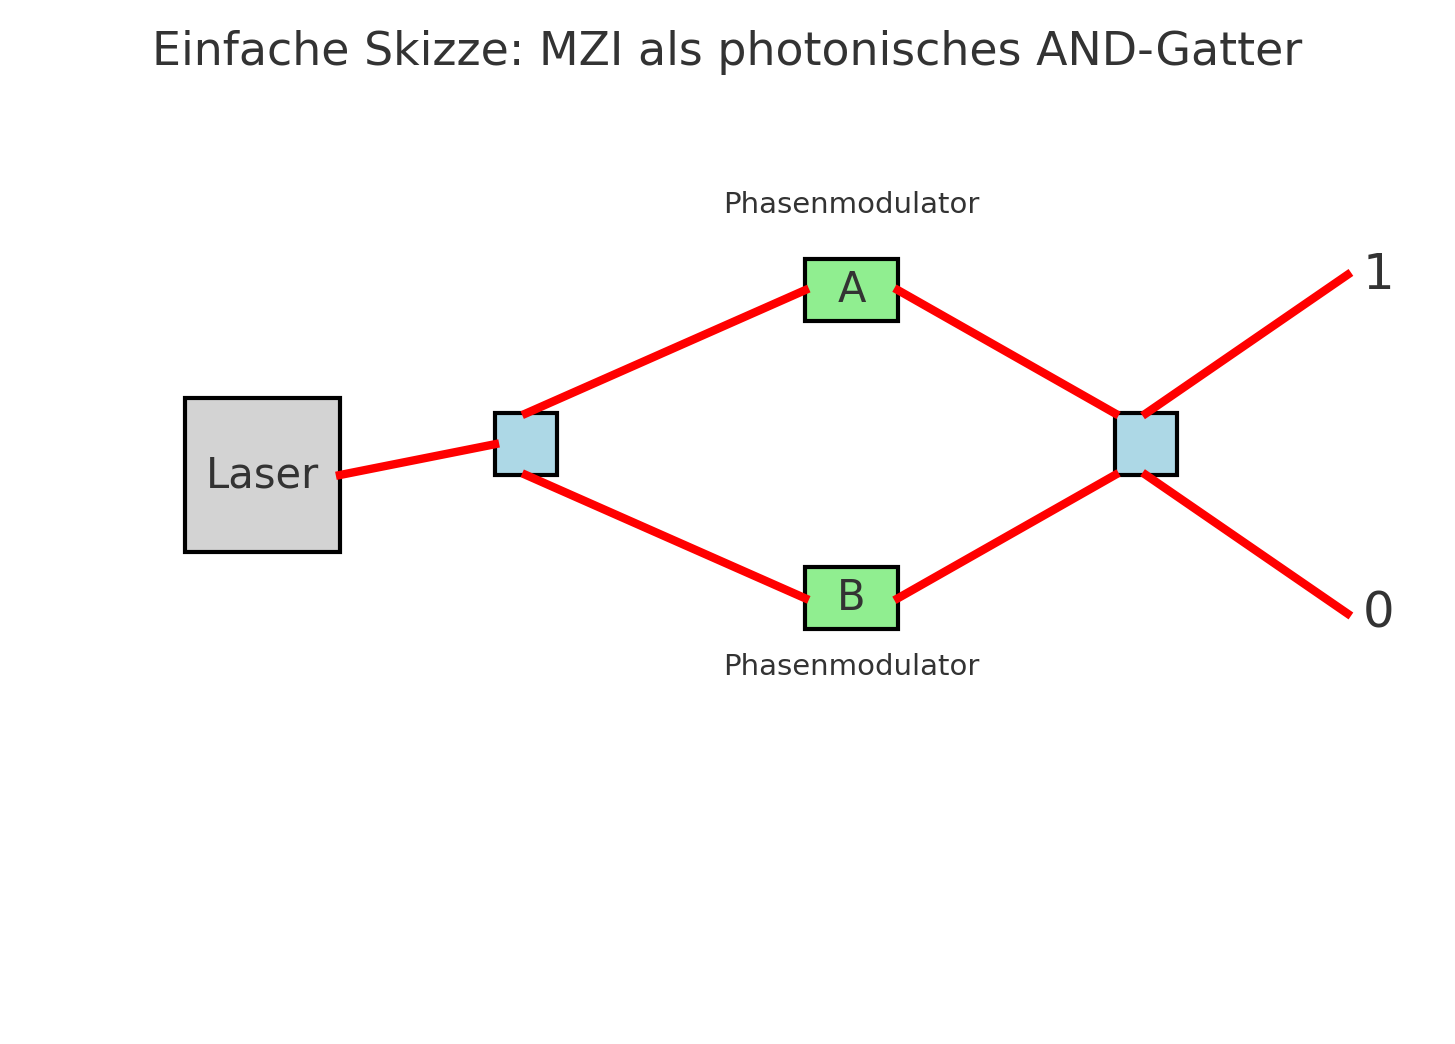
\includegraphics[width=0.75\textwidth]{bilder/mzi_and_simple.png}
	\caption{Simple schematic of a Mach--Zehnder interferometer with two phase modulators (\(A\) and \(B\)) acting as a photonic \textsc{AND} gate. Only if both modulators apply a phase shift of \(\pi\), the phases add to \(2\pi\) and light appears at the “1” output.}
	\label{fig:mzi_and_simple}
\end{figure}

\subsubsection{Challenges}
\index{Chip integration}
\index{Miniaturization}
\index{Electronics integration}

Despite the advantages, several open problems remain:
\begin{itemize}
	\item Efficient generation and control of single photons on a chip.
	\item Miniaturization of optical components to the nanometer scale.
	\item Integration with existing electronics.
\end{itemize}

\subsubsection{Summary}

Optical logic and photonic computers offer a fascinating possibility to increase computing power and reduce energy demand. Whether they will completely replace classical electronics or dominate only in special applications depends on solving the technical challenges.

\newpage
\noindent
\subsection{Photons in Fundamental Research}
\index{Boson}
\index{Cosmology}
\index{Cosmic microwave background}
\index{Bell test}
\index{Quantum tomography}
\index{Gravitational lens}
\index{Lorentz invariance}
\index{CPT symmetry}

Photons play a central role not only in technology but also in modern fundamental research. 
Their properties as massless, bosonic quantum objects make them ideal tools for studying fundamental questions of physics — from the smallest scales of quantum mechanics to cosmological distances.

\begin{itemize}
	\item \textbf{Testing quantum mechanics:} Experiments with single photons — such as double-slit experiments, Bell tests, or quantum tomography — test the limits and predictions of quantum mechanics with the highest precision.
	\item \textbf{Astrophysics and cosmology:} Photons from distant galaxies and the cosmic microwave background provide information on the origin and evolution of the universe.
	\item \textbf{Precision measurements:} Laser interferometers such as LIGO or Virgo detect tiny changes in length caused by gravitational waves — based on coherent photon beams.
	\item \textbf{Tests of fundamental symmetries:} Polarization, frequency, and flight time of photons are used to probe Lorentz invariance, CPT symmetry, and other fundamental principles.
\end{itemize}
\vspace{1em}
\begin{tcolorbox}[physikbox, title={Photons as Messengers of Natural Laws}, label={box:photonen_grundlagen}]
	\small
	Photons interact only weakly with their environment, move at the speed of light, and carry information about their source across billions of years and light-years.  
	This makes them unique messengers that provide insights into processes neither directly accessible nor reproducible — from the first moments after the Big Bang to the subtlest effects in quantum field theory.
\end{tcolorbox}
\newpage
\noindent
\begin{figure}[H]
	\centering
	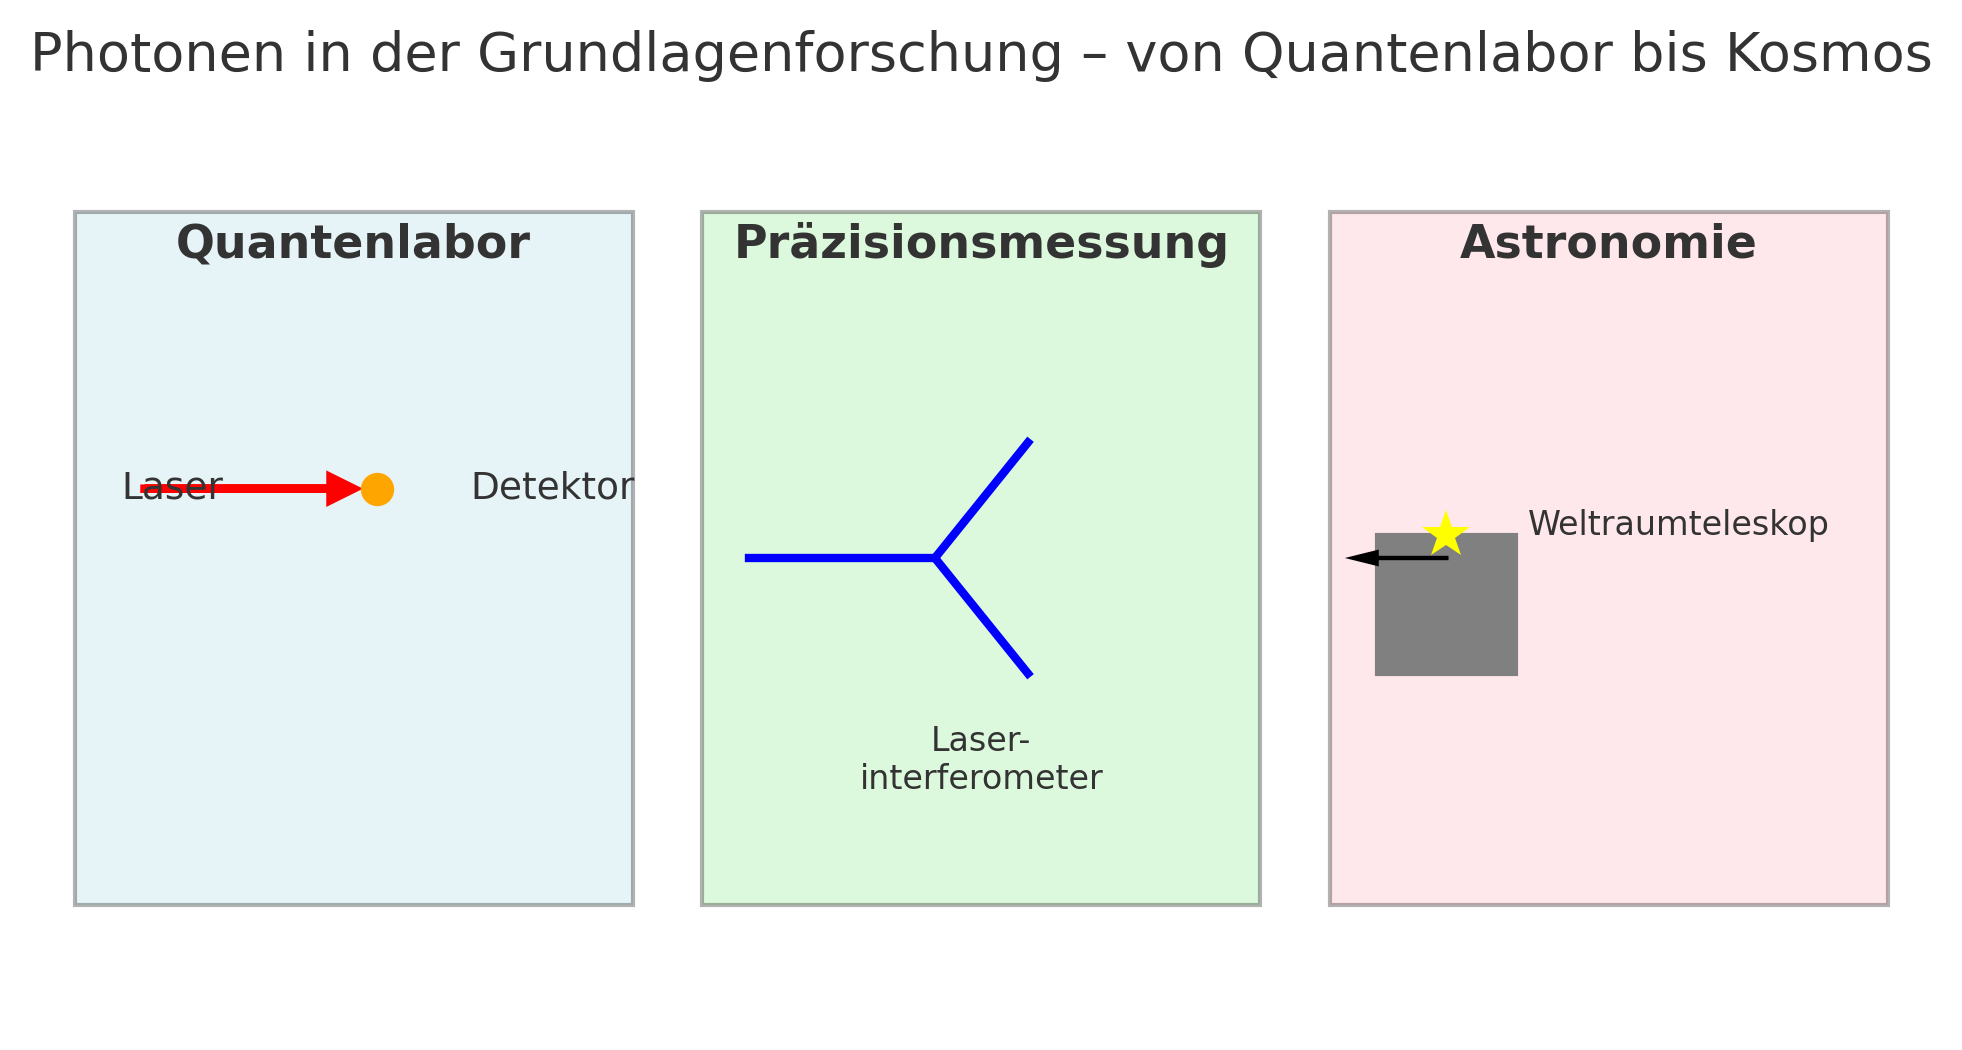
\includegraphics[width=0.9\textwidth]{bilder/photonen_grundlagenforschung.png}
	\caption{Photons in fundamental research: 
		from quantum labs and precision measurements to astronomy. 
		The illustration shows central fields of application: 
		experiments with single photons in the lab, laser interferometry for gravitational-wave detection, and space-based observations of stars and galaxies.}
	\label{fig:photonen_grundlagen}
\end{figure}

\subsubsection{Outlook}

Fundamental research with photons is far from complete. 
New detection methods, improved sources for single and entangled photons, and space-based experiments promise even deeper insights into the structure of natural laws.


\subsection{Outlook: Graviton, Dark Energy,\newline New Physics?}
\index{New physics}

Even though the photon as the quantum of light is well understood in modern physics, many fundamental questions remain — and photons often play a key role in answering them.

\begin{itemize}
	\item \textbf{The graviton:} The hypothetical exchange particle of gravitation has not yet been observed. Precise measurements with photons — via gravitational lenses or interferometry — could provide indirect evidence.
	\item \textbf{Dark energy:} The accelerated expansion of the universe points to an as-yet unknown form of energy. Photometry and spectroscopy of distant supernovae and galaxies use photons as the only information source to study this mysterious component.
	\item \textbf{New physics beyond the Standard Model:} High-precision experiments with photons could reveal deviations from established theories, such as tiny violations of Lorentz invariance or hints of additional spatial dimensions.
\end{itemize}

\begin{tcolorbox}[hypobox, title={What If the Photon Were Not the Only Massless Boson?}, label={box:photon_neue_physik}]
	\small
	The existence of additional massless exchange particles — such as the graviton — would fundamentally change our understanding of the fundamental forces.  
	Photon experiments could, through subtle effects such as deviations in light propagation or polarization patterns, provide the first hints of such new physics.
\end{tcolorbox}
\begin{figure}[H]
	\centering
	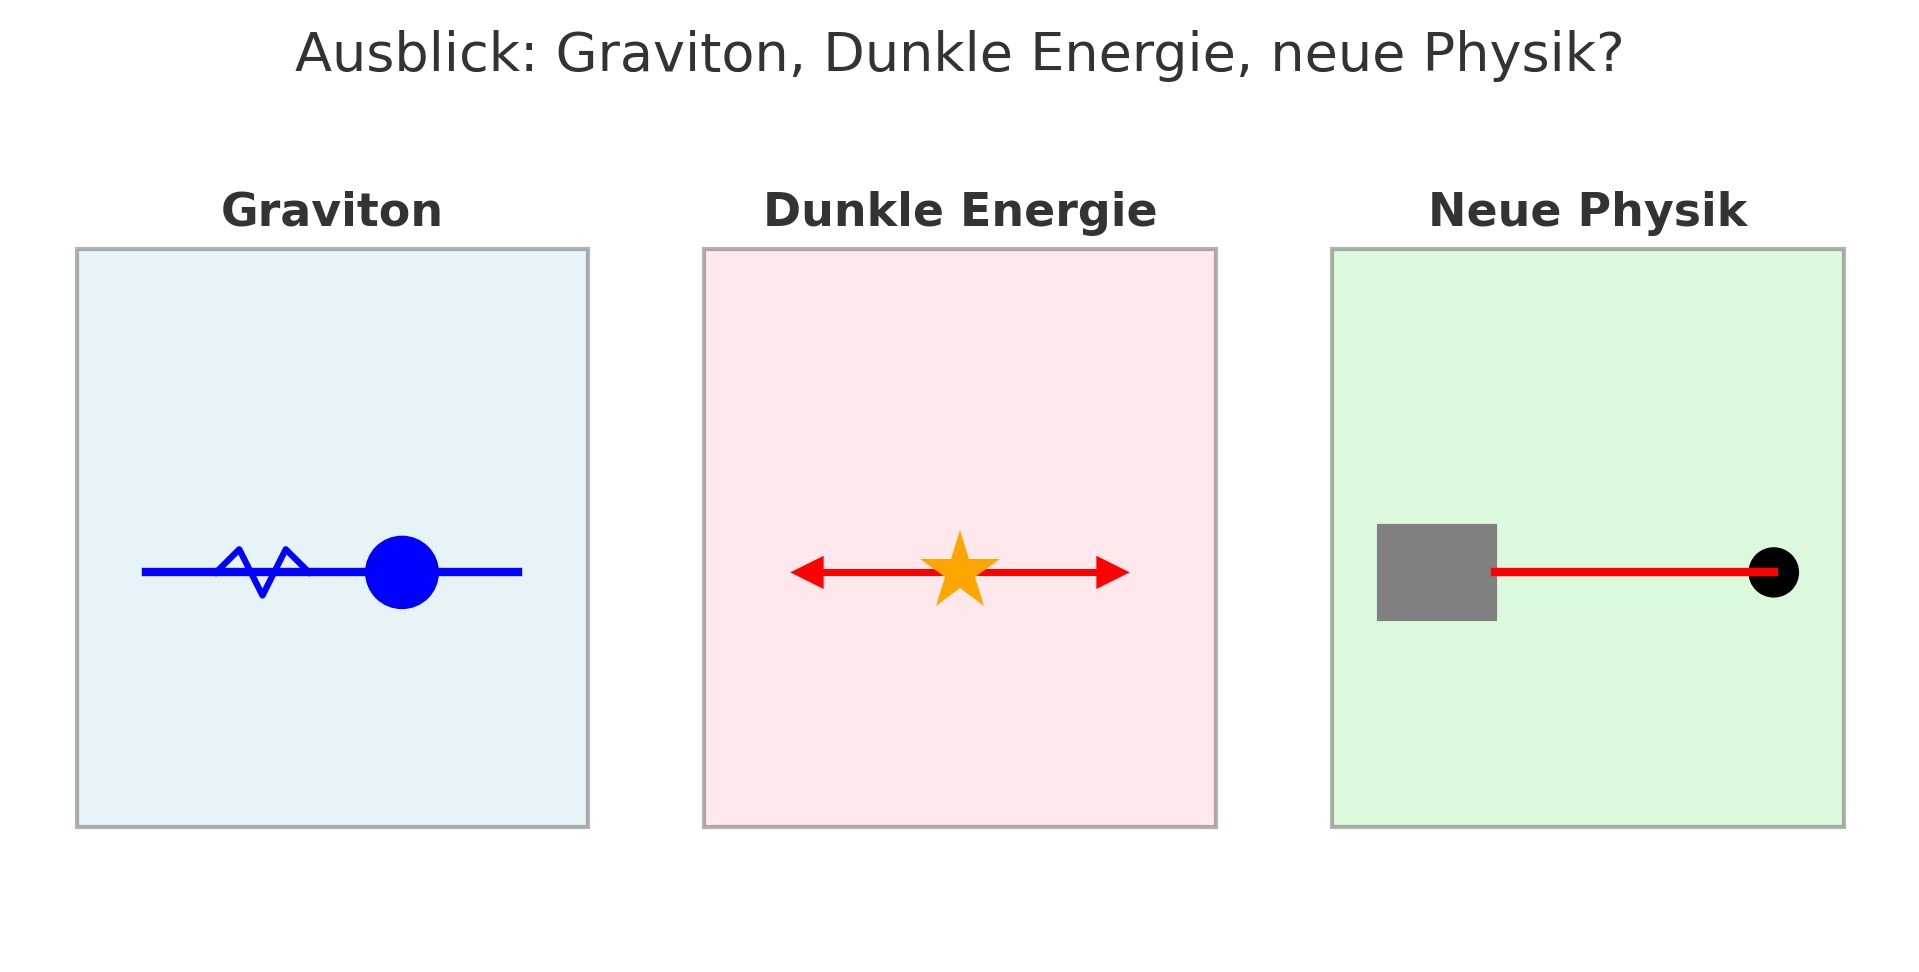
\includegraphics[width=0.9\textwidth]{bilder/photonen_ausblick_fixed.png}
	\caption{Symbolic outlook on open questions in physics:
		\textbf{left:} the hypothetical graviton as a possible candidate for another massless exchange particle;
		\textbf{center:} dark energy, recognizable in the accelerated expansion of the universe;
		\textbf{right:} laboratory experiments with photons searching for hints of new physics.}
	\label{fig:photonen_ausblick}
\end{figure}

\subsubsection{Outlook}

The future of photon research lies not only in technical applications but also in the photon’s role as a precise messenger of new natural laws.  
Space telescopes, gravitational-wave observatories, and laboratory experiments with unprecedented sensitivity could bring us closer to answering these fundamental questions.

\subsection{Conclusion}

Photons are far more than just carriers of light — they are tools, data transmitters, measuring instruments, and messengers of the fundamental laws of nature.  
From optical communication and precision metrology to photonic computers and the study of cosmic phenomena, their versatility is evident.  
The applications presented here make clear that photons not only form the foundation of modern technologies but are also crucial for exploring open questions of physics — from the nature of gravitation and dark energy to possible extensions of the Standard Model.  
The future of photon research therefore lies both in the further development of technical systems and in the search for new physics.

\medskip
\emph{The photon is not just a particle of light — it is a key to today’s technology and to the physics of tomorrow.}
\vspace{1em}
\begin{tcolorbox}[hypobox, title={What If We Could Fully Control Photons?}]
	\label{box:hypo_kapVII}
	A thought experiment: 
	\begin{itemize}
		\item Photonic chips could replace classical electronics — with nearly light-speed computations.
		\item Global quantum communication networks would be absolutely secure against eavesdropping.
		\item Single-photon labs could revolutionize medical diagnostics at the molecular level.
		\item Photons as “probes” could provide direct insights into dark matter or the structure of spacetime.
	\end{itemize}
	\medskip
	Such visionary scenarios go beyond today’s technology — they form the bridge to the next chapter on \emph{The Photon in the Standard Model and Visionary Applications}.
\end{tcolorbox}




	\chapter{The Photon in the Standard Model of Particle Physics}
\index{Photon}\index{Standard Model of Particle Physics}
\setcounter{section}{8}
\setcounter{subsection}{0}
\setcounter{subsubsection}{1}
\setcounter{secnumdepth}{3}
% Box style definitions
\tcbset{physikbox/.style={colback=blue!5!white, colframe=blue!75!black, fonttitle=\bfseries}}
\tcbset{mathebox/.style={colback=green!5!white, colframe=green!50!black, fonttitle=\bfseries}}
\tcbset{didaktikbox/.style={colback=yellow!5!white, colframe=yellow!50!black, fonttitle=\bfseries}}
\tcbset{hypobox/.style={colback=orange!5!white, colframe=orange!75!black, fonttitle=\bfseries}}
\tcbset{hinweisbox/.style={colback=gray!10!white, colframe=black!40!black, fonttitle=\bfseries}}

\subsection{The Standard Model: Overview}
\index{Gravitation}\index{Quantum Electrodynamics (QED)}\index{Weak Interaction}\index{Quantum Chromodynamics (QCD)}\index{Fermion}\index{Boson}\index{Gauge boson}\index{Higgs boson}\index{Higgs mechanism}\index{Gauge symmetry}\index{Lie group}\index{SU(3)}\index{SU(2)}\index{U(1)}\index{Electroweak theory}\index{Dark Matter}\index{Dark Energy}

The \textbf{Standard Model of Particle Physics} is a highly successful theory that describes the known fundamental particles and their interactions—with the exception of \textbf{gravitation}.  
It combines \textbf{quantum electrodynamics (QED)}, the \textbf{quantum theory of the weak interaction}, and \textbf{quantum chromodynamics (QCD)} into a consistent framework.

The fundamental building blocks are \textbf{fermions}, which form matter, and \textbf{bosons}, which act as exchange particles for the fundamental forces.  
Bosons are particles with integer spin that mediate the fundamental interactions.  
The gauge bosons include the \textbf{photon} (carrier of the electromagnetic interaction), the \textbf{$W^\pm$ and $Z^0$ bosons} (carriers of the weak interaction), and the \textbf{gluons} (carriers of the strong interaction).  
The \textbf{Higgs boson} plays a special role: it gives elementary particles their mass through the \textbf{Higgs mechanism}.

The interactions are described by \textbf{gauge symmetries}, formulated in the mathematical language of \textbf{Lie groups}.  
The Standard Model is based on the symmetry group \(\mathrm{SU(3)} \times \mathrm{SU(2)} \times \mathrm{U(1)}\).  
Each factor corresponds to a fundamental interaction:  
\(\mathrm{SU(3)}\) for the strong interaction, \(\mathrm{SU(2)} \times \mathrm{U(1)}\) for the \textbf{electroweak theory}.

Despite its success, the Standard Model is incomplete:  
It explains neither gravitation nor the nature of \textbf{dark matter} or \textbf{dark energy}.

\subsection{U(1) Gauge Symmetry and the Photon}
\index{U(1) gauge symmetry}\index{Abelian group}\index{Global symmetry}\index{Noether theorem}\index{Charge conservation}\index{Local symmetry}\index{Electromagnetic potential}\index{Gauge coupling}\index{Abelian gauge theory}

The electromagnetic interaction can be elegantly formulated as a \textbf{U(1) gauge symmetry}.  
The group \(\mathrm{U(1)}\) consists of all complex numbers of absolute value 1, expressed as \(e^{i\theta}\).  
It is an \textbf{abelian group}, i.e. the group operation (here: multiplication) is commutative.  
In mathematics, \(\mathrm{U(1)}\) is a \textbf{Lie group}, a continuous symmetry group parametrized by continuous parameters.

In quantum mechanics, a \textbf{global U(1) symmetry} describes the invariance of the wave function under a phase change \(\psi \to e^{i\alpha}\psi\).  
According to \textbf{Noether’s theorem}, this symmetry is directly linked to \textbf{charge conservation}.

If the symmetry is made \emph{local}—i.e. the phase angle \(\alpha\) may depend on space and time—one speaks of a \textbf{local U(1) gauge symmetry}.  
To preserve this invariance, a new field must be introduced: the electromagnetic potential \(A_\mu\).  
This field compensates the phase changes and leads to the \textbf{gauge coupling} between charged particles and the field.

Quantizing this field yields the \textbf{photon} as the massless \textbf{gauge boson} of the electromagnetic interaction.  
Its properties—especially masslessness and spin 1—follow directly from the structure of the U(1) symmetry.

The U(1) gauge theory is a special case of an abelian gauge theory and forms the electromagnetic sector of the \textbf{electroweak theory}.  
Its mathematical simplicity makes it an ideal starting point for understanding more complex theories such as \(\mathrm{SU(2)}\) or \(\mathrm{SU(3)}\).

\vspace{1em}
\begin{tcolorbox}[didaktikbox, title=U(1) explained intuitively]
	\label{box:u1_kreis}
	\small
	\begin{minipage}{0.35\textwidth}
		\centering
		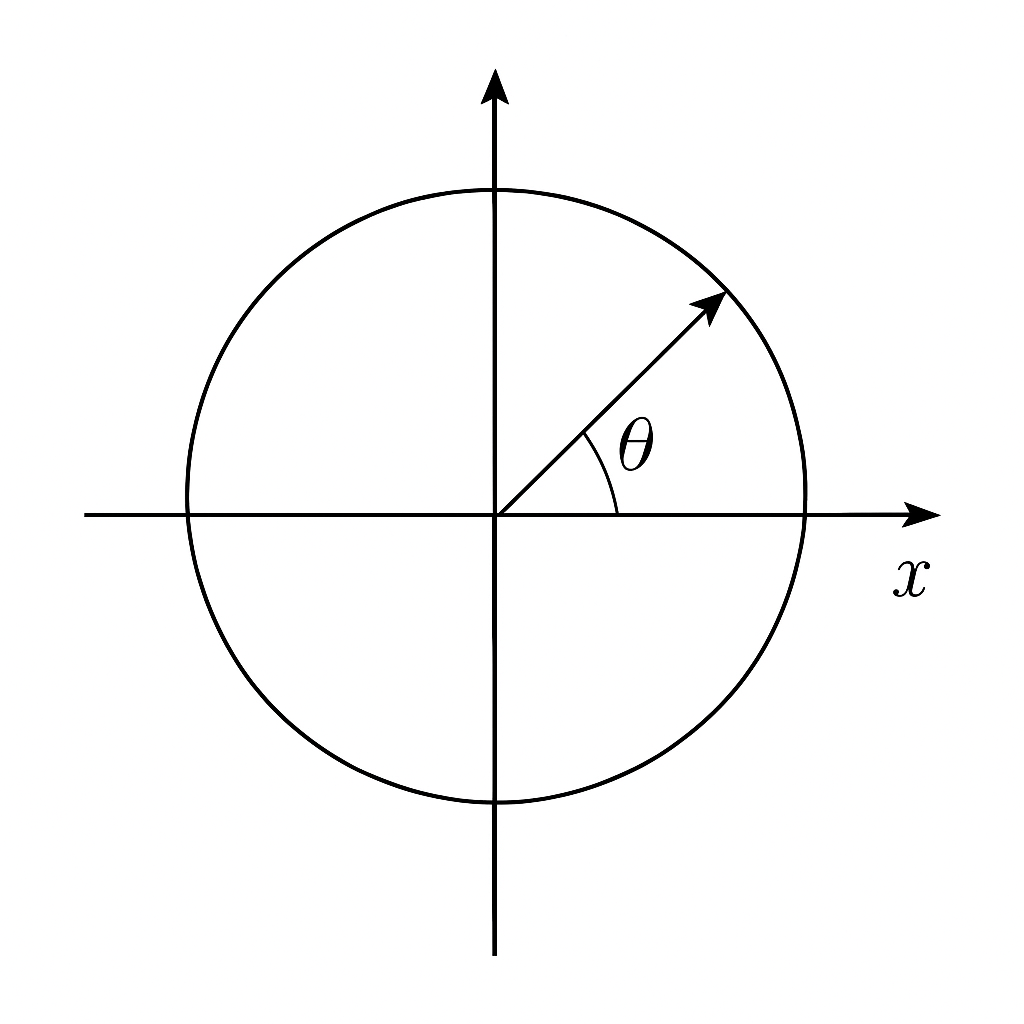
\includegraphics[width=\linewidth]{bilder/u1_kreis.png}
	\end{minipage}%
	\begin{minipage}{0.63\textwidth}
		The group \(\mathrm{U(1)}\) can be pictured as all possible 
		rotations on a circle.  
		Each point on the circle is defined by an angle \(\theta\).  
		In quantum mechanics this corresponds to a phase change of the wave function
		– the distance to the origin always stays the same, only the direction changes.
	\end{minipage}
\end{tcolorbox}

\subsection{Electroweak Unification}
\index{Electroweak theory}\index{Glashow, Sheldon}\index{Salam, Abdus}\index{Weinberg, Steven}\index{Nobel Prize in Physics}\index{SU(2)}\index{Weinberg angle}\index{Higgs mechanism}\index{CERN}

The \textbf{electroweak theory} unifies the \textbf{electromagnetic interaction} and the \textbf{weak interaction} in a single theoretical framework.  
It was developed in the late 1960s by \textbf{Sheldon Glashow}, \textbf{Abdus Salam}, and \textbf{Steven Weinberg} and forms a central part of the \textbf{Standard Model of Particle Physics}.  
For this achievement they received the \textbf{Nobel Prize in Physics} in 1979.

Mathematically, the electroweak theory is based on the symmetry group \(\mathrm{SU(2)} \times \mathrm{U(1)}\).  
The \(\mathrm{SU(2)}\) symmetry describes the weak interaction with its three gauge bosons \(W^1, W^2, W^3\), while the \(\mathrm{U(1)}\) symmetry represents the electromagnetic part.  
Through a mixing (\emph{Weinberg angle}) of the fields \(W^3\) and \(B\) (the U(1) boson), the massless \textbf{photon} and the neutral \textbf{\(Z^0\) boson} emerge.

The electroweak symmetry is spontaneously broken by the \textbf{Higgs mechanism}.  
This gives the \(W^\pm\) and \(Z^0\) bosons mass, while the photon remains massless.  
This property is a direct manifestation of the remaining unbroken U(1) symmetry of electrodynamics.

The experimental confirmation of the electroweak theory came in the early 1980s at \textbf{CERN} through the direct detection of the \(W\) and \(Z\) bosons.  
This discovery is regarded as one of the greatest successes of modern particle physics.

\vspace{1em}
\begin{tcolorbox}[didaktikbox, title=From \(W^3\) and \(B\) to the Photon]
	\label{box:weinberg_mischung}
	\small
	\begin{minipage}{0.35\textwidth}
		\centering
		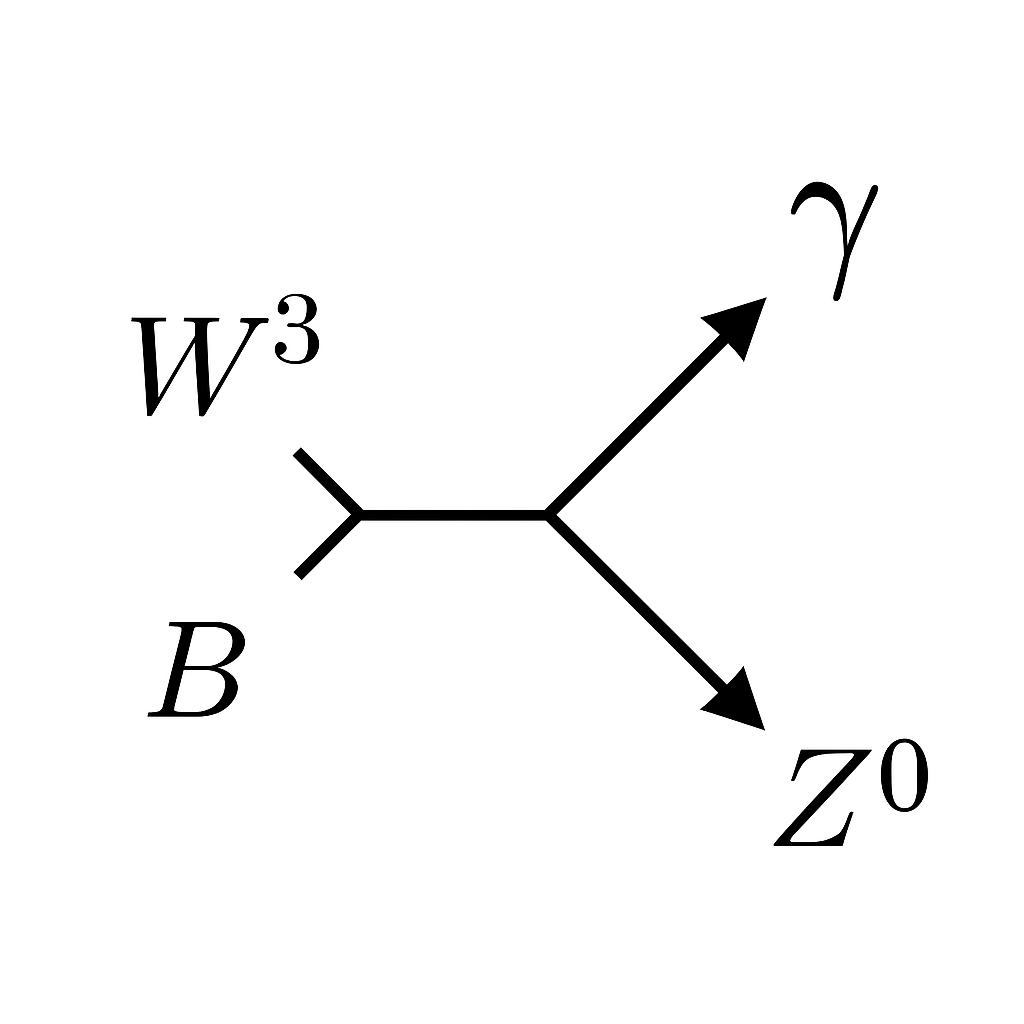
\includegraphics[width=\linewidth]{bilder/weinberg_mischung.png}
	\end{minipage}%
	\begin{minipage}{0.63\textwidth}
		In electroweak theory, the \textbf{photon} \(\gamma\) and the neutral 
		\(\mathbf{Z^0}\) boson arise through a mixing of the fields \(W^3\) and \(B\) 
		– described by the \textbf{Weinberg angle} \(\theta_W\).  
		\vspace{0.3em}
		
		Mathematically:
		\[
		\begin{aligned}
			\gamma &= \phantom{-}\cos\theta_W \, B + \sin\theta_W \, W^3 \\
			Z^0    &= -\sin\theta_W \, B + \cos\theta_W \, W^3
		\end{aligned}
		\]
		This rotation of fields explains why the photon remains massless, while 
		the \(Z^0\) boson acquires mass.
	\end{minipage}
\end{tcolorbox}
\newpage
\noindent
\subsection{Why Is the Photon Massless?}
\index{Photon mass}\index{Lagrangian density}\index{Range of electromagnetic interaction}\index{Compton wavelength}

Within the \textbf{Standard Model of Particle Physics}, the \textbf{photon} is a massless \textbf{gauge boson} of the electromagnetic interaction.  
Its masslessness is a direct consequence of the unbroken \textbf{U(1) gauge symmetry} in \textbf{quantum electrodynamics (QED)}.

In the \textbf{Higgs mechanism}, which gives the \(W^\pm\) and \(Z^0\) bosons mass, exactly one gauge symmetry remains unbroken: the U(1) symmetry of electrodynamics.  
The associated gauge field is identified with the photon—and since unbroken gauge symmetries always lead to massless exchange particles, the photon has no rest mass.

Mathematically this appears in the Lagrangian density of the electromagnetic field: no mass term of the form \(\frac{1}{2} m^2 A_\mu A^\mu\) occurs.  
Such a term would violate gauge invariance and is therefore forbidden.

Experimental bounds on a possible photon mass are extremely strict:  
Measurements set an upper limit of less than \(10^{-18}\,\mathrm{eV}/c^2\).  
Practically the photon is perfectly massless—an essential property for the infinite range of the electromagnetic force.

\vspace{1em}
\begin{tcolorbox}[hinweisbox, title=Masslessness and range]
	\label{box:reichweite_masselos}
	\small
	The range of a fundamental interaction is directly linked to the mass of its exchange particle.  
	\begin{itemize}
		\item \textbf{Massless exchange particles} (e.g. photons) mediate forces with unlimited range.  
		\item \textbf{Massive exchange particles} (e.g. \(W^\pm\) and \(Z^0\) bosons) mediate forces with finite range, determined by the \emph{Compton wavelength} \(\lambda_C = \hbar/(mc)\).
	\end{itemize}
	For the photon, its masslessness implies the infinite range of the electromagnetic interaction.
\end{tcolorbox}
\newpage
\noindent
\vspace{1em}
\begin{tcolorbox}[physikbox, title=Massless photon and spin correlations over long distances]
	\label{box:photon_spin_reichweite}
	\small
	A massless photon has no range limitation in transmitting its quantized properties.  
	This has two essential consequences:
	\begin{itemize}
		\item \textbf{Infinite interaction range:} The electromagnetic force acts in principle over arbitrary distances.
		\item \textbf{Conservation of spin direction (polarization):} Since the photon is massless and travels at the speed of light, its spin or polarization orientation is preserved even across cosmological distances. 
	\end{itemize}
	In entangled quantum states this means that the polarization correlations of two photons remain measurable even when they are far apart—a result of the combination of masslessness and quantum entanglement.
\end{tcolorbox}

\subsection{Comparison with Other Gauge Bosons}
\index{W boson}\index{Z boson}\index{Gluon}\index{Confinement}\index{Graviton}

In the \textbf{Standard Model of Particle Physics} there are several \textbf{gauge bosons} that mediate fundamental interactions.  
The \textbf{photon} differs from them in essential properties:

\begin{itemize}
	\item \textbf{Photon (QED):} Massless, spin \(1\), mediates the \textbf{electromagnetic interaction}.  
	Range: infinite.
	
	\item \(\mathbf{W^\pm}\) and \(\mathbf{Z^0}\) \textbf{bosons} (electroweak theory):  
	Spin \(1\), heavy masses (\(\approx 80{-}91\,\mathrm{GeV}/c^2\)), range: about \(10^{-18}\,\mathrm{m}\).  
	Mediators of the \textbf{weak interaction}.
	
	\item \textbf{Gluons} (QCD):  
	Spin \(1\), formally massless, mediate the \textbf{strong interaction}.  
	Effective range is very limited due to \textbf{confinement}—gluons never appear as free particles.
	
	\item \textbf{Graviton} (hypothetical):  
	Spin \(2\), massless, would mediate gravitation.  
	Not experimentally confirmed.
\end{itemize}

The decisive difference:  
Only the photon appears as a freely measurable, massless exchange particle with unlimited range.  
W and Z bosons are massive and thus short-range, gluons are massless but confined in bound states.

\vspace{1em}
\begin{tcolorbox}[hinweisbox, title=Comparison of gauge bosons]
	\label{box:eichbosonen_vergleich}
	\small
	
	\resizebox{\linewidth}{!}{%
		\begin{tabular}{lcccc}
			\textbf{Particle} & \textbf{Spin} & \textbf{Mass} & \textbf{Range} & \textbf{Interaction} \\
			\hline
			Photon & 1 & 0 & infinite & electromagnetic \\
			\(W^\pm\) & 1 & \(\approx 80\,\mathrm{GeV}/c^2\) & \(10^{-18}\,\mathrm{m}\) & weak \\
			\(Z^0\) & 1 & \(\approx 91\,\mathrm{GeV}/c^2\) & \(10^{-18}\,\mathrm{m}\) & weak \\
			Gluon & 1 & 0 & \emph{effectively short} & strong (confinement) \\
			Graviton (hyp.) & 2 & 0 & infinite & gravitation \\
		\end{tabular}%
	}
	
\end{tcolorbox}

\subsection{Open Questions and Extensions}
\index{Grand Unified Theory (GUT)}\index{String theory}\index{Quantum gravity}

Despite the success of the \textbf{Standard Model of Particle Physics}, fundamental questions remain unanswered that also involve the \textbf{photon} or could extend its theoretical framework:

\begin{itemize}
	\item \textbf{Photon mass:}  
	Experimentally the photon is considered massless, but an extremely tiny, so far unmeasurable mass cannot be excluded.  
	Future precision measurements may further constrain this limit—or surprisingly reveal a finite mass.
	
	\item \textbf{Interaction with dark matter:}  
	Whether photons couple in any way to dark matter is unknown.  
	Direct and indirect searches may provide hints in the future.
	
	\item \textbf{Unified theories:}  
	In models beyond the Standard Model—such as \textbf{Grand Unified Theories (GUT)} or \textbf{string theories}—the photon is part of a larger symmetry structure.  
	These models may predict new properties or partner particles.
	
	\item \textbf{Quantum gravity:}  
	A consistent theory uniting gravitation with the quantum fields of particle physics is still missing.  
	The interaction of the photon with hypothetical \textbf{gravitons} or with the structure of spacetime on the smallest scales remains largely unexplored.
	
	\item \textbf{New symmetries or particles:}  
	Extensions of the Standard Model could involve additional gauge bosons or symmetries that influence the role of the photon.
\end{itemize}

Answering these questions will require a combination of precise experiments, new observational technologies, and theoretical breakthroughs.  
Thus, the photon remains not only a central tool of physics but also a key to possible new physical worlds.

\subsection{Conclusion}
\subsubsection*{The Photon – Particle, Wave, and Window to the Future}
\phantomsection
The \textbf{photon} has played a unique role in the history of physics:  
It was the key to the birth of quantum theory, the starting point for the development of \textbf{quantum electrodynamics (QED)}, and remains an indispensable tool of both experimental and theoretical research.

From the \textbf{photoelectric effect} to \textbf{Compton scattering} to modern applications such as \textbf{quantum communication} and \textbf{photonics}, the photon has not only shaped our physical models but also enabled technologies that transform daily life.

Within the \textbf{Standard Model of Particle Physics}, the photon embodies an unbroken \textbf{U(1) gauge symmetry}—a mathematical elegance expressed in its masslessness and infinite range.  
At the same time, the open questions show that we are still far from a complete understanding.


The photon unites fundamental properties of nature:
\begin{itemize}
	\item \textbf{Wave and particle} in a single quantum description.
	\item \textbf{Massless messenger} with infinite range.
	\item \textbf{Precise probe} in astronomy, particle physics, and quantum optics.
	\item \textbf{Key actor} in future technologies such as quantum computers and photonic circuits.
\end{itemize}

Its dual role as theoretical foundation and practical tool makes the photon one of the most fascinating objects in physics.  
It is not only a component of our physical worldview but also a gateway to yet unknown aspects of the universe—a gateway that we will continue to push open in the decades ahead.

Even though the photon appears in a clear and consistent role in the Standard Model, 
it simultaneously symbolizes the limits of this theory.  
To highlight this dual function—as foundation and as bridge to new physics— 
we conclude with a didactic summary and then take a speculative look into the future.
\newpage
\noindent
\vspace{1em}
\begin{tcolorbox}[didaktikbox, title=Didactic conclusion: The photon in the Standard Model]
	\label{box:didaktik_kapVIII}
	The photon is not only a tool of quantum optics and modern technology, 
	but also a key figure in the theoretical foundation of physics.  
	
	\medskip
	\textbf{Core message:}  
	Its role as a massless gauge boson of the unbroken U(1) symmetry combines mathematical elegance, 
	experimental precision, and cosmic range.  
	Thus the photon exemplifies both the strength—and the limits—of the Standard Model.
\end{tcolorbox}

\vspace{1em}
\begin{tcolorbox}[hypobox, title={What if the Standard Model were only a stepping stone?}]
	\label{Merksatz zum Photon}
	A thought experiment:
	\begin{itemize}
		\item If photons could interact with dark matter, our understanding of cosmology would be revolutionized.  
		\item Detecting a tiny photon mass would fundamentally change the structure of electrodynamics.  
		\item New symmetries or hidden partner particles of the photon could appear in an extended theory beyond the Standard Model.  
		\item Perhaps the photon is even the key to linking quantum field theory and gravitation.  
	\end{itemize}
	
	\medskip
	Such speculative perspectives go beyond the Standard Model—and open the door 
	to a future chapter on \emph{new physics}.
\end{tcolorbox}

	\cleardoublepage
\appendix
\renewcommand{\thechapter}{A}
\renewcommand{\thesection}{\Alph{chapter}.\arabic{section}}


\chapter{Mathematical Background and Derivations}
\label{anhangA}

This appendix provides a formal and mathematical deepening of the physical
concepts discussed in the main text. The aim is to preserve the didactic
readability of the chapters while at the same time giving interested readers
access to the complete derivations.  

The sections are thematically structured according to the central properties
of the photon, including the energy–momentum relation, the mass hypothesis,
helicity, and polarization.\index{Photon!properties} In this way, the appendix builds a bridge between
the intuitive explanations in the main text and the mathematical rigor of
quantum field theory.

%\section{Chapter I}
\section{Energy–Momentum Relation of the Photon}\index{Energy–momentum relation!photon}
\label{anhangA:energie_impuls}

This section formally derives why a photon has the energy
\[
E = h f
\]
and the momentum
\[
p = \frac{h}{\lambda}
\]
Starting from Maxwell’s equations and their wave equation, it is shown via the
Poynting vector\index{Poynting vector} and the energy density of the electromagnetic field that
quantization of the fields leads to discrete energy portions. This derivation
supplements the intuitive presentation in the main text (Chapter~I).

\section{The Electromagnetic Field in the Relativistic Formulation}\index{Electromagnetic field!relativistic formulation}\index{Field strength tensor}\index{Lagrangian density}
\label{anhangA:feldtheorie}

Here we introduce the formal description of the electromagnetic field:

\begin{itemize}
	\item Four-potential $A^\mu = (\phi, \vec{A})$\index{Four-potential}
	\item Field strength tensor $F^{\mu\nu} = \partial^\mu A^\nu - \partial^\nu A^\mu$\index{Field strength tensor}
	\item Antisymmetry property $F^{\mu\nu} = -F^{\nu\mu}$
	\item Lagrangian density\index{Lagrangian density}
	\[
	\mathcal{L} = -\frac{1}{4} F_{\mu\nu}F^{\mu\nu}
	\]
	\item Connection to quantization: photon as the gauge boson of $U(1)$
	electromagnetism\index{Gauge boson!U(1)}
\end{itemize}

This provides the mathematical foundation for the statement in the main text
that photons are “excitations of the electromagnetic field.”

\section{Formal Description of Entangled Photons}\index{Photons!entanglement}\index{Dirac notation}\index{SPDC (spontaneous parametric down-conversion)}
\label{anhangA:verschr}

The experiments on the generation of entangled photon pairs (SPDC) presented
in the main text (Chapter~I) can be formally described in Dirac notation. A
typical entangled polarization state pair is given by:

\[
|\psi\rangle = \frac{1}{\sqrt{2}}\big( |H\rangle_A \otimes |V\rangle_B +
|V\rangle_A \otimes |H\rangle_B \big)
\]

\begin{itemize}
	\item $|H\rangle$: horizontally polarized state
	\item $|V\rangle$: vertically polarized state
	\item Indices $A, B$: the two photons
\end{itemize}

This formalism makes the correlations observed in the experiment transparent
and shows why classical hidden-variable models are not sufficient.
%\section{Chapter II}
\section{Derivation of the Rayleigh–Jeans Law}\index{Rayleigh–Jeans law!derivation}\index{Rayleigh, Lord}\index{Jeans, James}\index{Ultraviolet catastrophe}
\label{anhangA:rayleigh}

The Rayleigh–Jeans law arises when the electromagnetic modes in a cavity are
treated as harmonic oscillators:

\begin{enumerate}
	\item Count the number of standing waves in the cubic volume $V$.
	\item Each mode has two polarization directions.
	\item According to the equipartition principle of classical thermodynamics,
	each degree of freedom in equilibrium contributes the mean energy $kT$.
\end{enumerate}

The number of modes between the frequencies $\nu$ and $\nu + d\nu$ is
\[
g(\nu)\, d\nu = \frac{8\pi V \nu^2}{c^3}\, d\nu.
\]

Multiplied by $kT$, this yields the spectral energy density
\[
u(\nu, T) = \frac{8\pi \nu^2}{c^3}\, kT,
\]
which, in wavelength form, becomes $u(\lambda, T) = \tfrac{8\pi kT}{\lambda^4}$.
The law is accurate at long wavelengths but diverges for $\lambda \to 0$ – the
so-called \emph{ultraviolet catastrophe}.

\section{Wien’s Radiation Law}\index{Wien’s displacement law}\index{Wien, Wilhelm}
\label{anhangA:wien}

In 1896 Wilhelm Wien derived an approximation for blackbody radiation.
His reasoning was based on:

\begin{itemize}
	\item Thermodynamic considerations: adiabatic compression of a cavity shifts
	the radiation spectrum.
	\item Dimensional analysis: the intensity depends on $T$ and $\lambda$ and
	must have the correct units.
\end{itemize}

The result was
\[
u(\lambda, T) = \frac{c_1}{\lambda^5}\,
\exp\!\left(-\frac{c_2}{\lambda T}\right),
\]
with constants $c_1, c_2$, which were only fully understood through Planck’s
approach. Wien’s law is valid in the UV region but fails at long wavelengths.

\section{Derivation of Planck’s Radiation Law}\index{Planck’s radiation law!derivation}\index{Planck, Max}
\label{anhangA:planck}

Planck combined the limiting cases of Rayleigh–Jeans and Wien and introduced
the quantization of energy:

\begin{itemize}
	\item An oscillator can only take on energies $E_n = nh\nu$.
	\item The occupation probability follows the Boltzmann distribution.
\end{itemize}

The mean energy per oscillator is
\[
\langle E \rangle = \frac{h\nu}{e^{h\nu/kT} - 1}.
\]

Multiplied by the mode number
$g(\nu)\, d\nu = \tfrac{8\pi V \nu^2}{c^3}\, d\nu$
this gives the energy density
\[
u(\nu, T) = \frac{8\pi \nu^2}{c^3}\,
\frac{h\nu}{e^{h\nu/kT} - 1}.
\]

This is \textbf{Planck’s radiation law}, which agrees with experiment at all
frequencies.

\section{Mathematical Description of the Photoelectric Effect}\index{Photoelectric effect!mathematical description}
\label{anhangA:photoeffekt}

In the photoelectric effect, an electron in a metal absorbs a photon with
energy $E_\gamma = h\nu$. To release the electron from the metal, the
\emph{work function} $A$ must be overcome. The excess energy goes into the
electron’s kinetic energy:

\[
E_\text{kin} = h\nu - A.
\]

This leads to a \emph{threshold frequency}
\[
\nu_\text{min} = \frac{A}{h},
\]
below which no electrons are emitted – independent of light intensity.
This linear relation between electron energy and light frequency was confirmed
precisely in Millikan’s experiments (1916).\index{Millikan, Robert A.}
%\section{Chapter III}
\section{Photon Momentum}\index{Photon!momentum}\index{Energy–momentum relation}
\label{anhangA:impuls}

The momentum of a photon can be derived from the relativistic
energy–momentum relation. For arbitrary particles,
\[
E^2 = (pc)^2 + (m_0 c^2)^2 ,
\]
where $E$ is the energy, $p$ the momentum, $c$ the speed of light, and $m_0$ the rest mass.

\begin{itemize}
	\item For massless particles ($m_0 = 0$) this equation reduces to
	\[
	E = p c.
	\]
	
	\item For the photon, the quantization condition holds simultaneously:
	\[
	E = h f = \frac{h c}{\lambda}.
	\]
	
	\item Equating both expressions for $E$ immediately yields
	\[
	p = \frac{E}{c} = \frac{h}{\lambda}.
	\]
\end{itemize}

\noindent
Thus, the momentum of a photon is directly linked to its wavelength. This relation is one of the central bridges between the wave and particle description of light.

\section{Energy–Momentum Relation of the Photon}\index{Photon!mass hypothesis}\index{Photon!masslessness}\index{Energy–momentum relation}
\label{anhangA:masse}

For relativistic particles, the general energy–momentum relation is
\[
E^2 = (pc)^2 + (m c^2)^2.
\]

\begin{itemize}
	\item \textbf{Massless photon:}  
	Setting $m=0$ immediately gives
	\[
	E = p c.
	\]
	This is consistent with the relations $E = h f$ and $p = h/\lambda$.
	
	\item \textbf{Hypothetically massive photon:}  
	If the photon had a rest mass $m_\gamma \neq 0$, then
	\[
	E^2 = (p c)^2 + (m_\gamma c^2)^2.
	\]
	Such a photon would always move slower than $c$, and the speed of light would no longer be universally constant.  
	Even minimal deviations from $m=0$ would be revealed in precision experiments.
\end{itemize}

Experimentally, only an upper bound for the photon mass has been established so far. Current limits are
\[
m_\gamma < 10^{-18}\,\text{eV}/c^2,
\]
which effectively means that the photon is considered massless.

\section{Helicity of the Photon}\index{Photon!helicity}\index{Spin}
\label{anhangA:helizitaet}

The photon has spin $s=1$, but due to its masslessness not all three spin projections ($m_s=-1,0,+1$) are physically realizable. 

\begin{itemize}
	\item \textbf{General spin-1 state:}  
	For massive spin-1 particles, three polarization states are possible,
	corresponding to the projections $m_s=-1,0,+1$ onto the direction of motion.
	
	\item \textbf{Massless photon:}  
	Since the photon has no rest mass, there is no rest frame in which the spin orientation can be defined independently of the momentum vector.  
	Mathematically, the gauge invariance of Maxwell’s equations (or of the QED formalism) enforces the vanishing of the longitudinal component ($m_s=0$).
	
	\item \textbf{Helicity states:}  
	Two possible states remain:
	\begin{align*}
		\lambda &= +1 \quad \text{(right-handed, right circular polarization)}\\
		\lambda &= -1 \quad \text{(left-handed, left circular polarization)}
	\end{align*}
	
	These are called the two helicity states of the photon.
\end{itemize}

\noindent
Thus, the photon is a two-state massless boson whose degrees of freedom are fully described by the two possible helicities.

\section{Polarization of the Photon}\index{Photon!polarization}\index{Dirac notation}\index{Jones vector}
\label{anhangA:polarisation}

Polarization describes the transverse oscillation direction of a photon’s electric field. Formally, this degree of freedom can be represented in two ways:

\begin{itemize}
	\item \textbf{Dirac notation:}  
	In quantum mechanics, polarization states are written as basis vectors in a two-dimensional Hilbert space:  
	\[
	|H\rangle = \begin{pmatrix}1 \\ 0\end{pmatrix}, \qquad
	|V\rangle = \begin{pmatrix}0 \\ 1\end{pmatrix},
	\]
	where $|H\rangle$ stands for horizontal and $|V\rangle$ for vertical polarization.  
	Arbitrary polarization states can be expressed as linear combinations:  
	\[
	|\psi\rangle = \alpha |H\rangle + \beta |V\rangle, \quad |\alpha|^2 + |\beta|^2 = 1.
	\]
	
	\item \textbf{Jones vectors:}  
	In classical optics, the same state is described by \emph{Jones vectors}:  
	\[
	\vec{E} = \begin{pmatrix} E_x \\ E_y \end{pmatrix},
	\]
	where $E_x$ and $E_y$ are the complex amplitudes of the electric field components in the $x$- and $y$-directions.  
	Here too, normalizing the intensity corresponds to normalizing the state vector in Dirac notation.
\end{itemize}

\noindent
Both descriptions are equivalent — Dirac notation emphasizes the quantum mechanical state space, while Jones vectors reflect the classical electromagnetic wave optics.  
Linking these representations is a central tool in quantum optics.
%\section{Chapter IV}
\section{Derivation of Einstein’s Photoelectric Equation}
\label{anhangA:photoeffekt}

Einstein’s equation\index{Einstein’s equation}\index{Photoelectric effect}
\[
E_{\text{kin}} = h \nu - A
\]
follows from a simple energy balance between a photon\index{Photon} and an electron.\index{Electron}

\begin{enumerate}
	\item A photon carries the energy
	\[
	E_{\text{photon}} = h \nu,
	\]
	where \( h \) is Planck’s constant\index{Planck’s constant}\index{Planck, Max} and \( \nu \) is the frequency\index{Frequency} of the incident light.
	
	\item To liberate an electron from a metal, the \textbf{work function} \( A \)\index{Work function} must be overcome. This corresponds to the minimal binding energy of electrons in the solid.
	
	\item If energy remains after overcoming \( A \), it appears as the electron’s kinetic energy:\index{Kinetic energy}
	\[
	E_{\text{kin}} = E_{\text{photon}} - A.
	\]
	
	\item Hence, directly:
	\[
	E_{\text{kin}} = h \nu - A.
	\]
\end{enumerate}

\textbf{Remark.}  
If a retarding (stopping) voltage \( U \)\index{Stopping potential} is applied, then
\[
eU = h \nu - A,
\]
where \( e \) is the elementary charge.\index{Elementary charge} This form allows a direct experimental determination of \( h \) by measuring the stopping potential as a function of the frequency.

\section{Planck–Einstein Relation \texorpdfstring{$E = h\nu$}{E = hν}}
\label{anhangA:planckEinstein}
\index{Planck–Einstein relation}

\textbf{Goal.} Justify why a single light quantum (photon) carries the energy
\[
E = h\nu = \hbar \omega .
\]

\subsection*{Route 1: Quantizing the normal modes of the electromagnetic field.}
\phantomsection
The free electromagnetic field\index{Electromagnetic field} in a volume \(V\) can be decomposed into plane normal modes with angular frequencies \(\omega_{\mathbf{k}}\). Each mode is a harmonic oscillator\index{Harmonic oscillator} with Hamiltonian
\[
\hat H_{\mathbf{k}}=\hbar \omega_{\mathbf{k}}\!\left(\hat a_{\mathbf{k}}^\dagger \hat a_{\mathbf{k}}+\tfrac12\right).
\]
The eigenvalues are \((n+\tfrac12)\hbar\omega_{\mathbf{k}}\), \(n\in \mathbb{N}_0\). 
An excitation \(\Delta n = 1\) raises the energy by \(\Delta E = \hbar \omega\). 
We identify this increase with \emph{one photon} in that mode:
\[
E_{\text{photon}}=\hbar\omega=h\nu.
\]

\subsection*{Route 2: From Planck’s quantum hypothesis to Einstein’s light quantum.}
\phantomsection
Planck\index{Planck, Max} postulated in 1900 discrete energies \(E_n=n h\nu\) for matter oscillators. 
Einstein\index{Einstein, Albert} in 1905 applied quantization to the \emph{radiation field} itself: the energy of radiation behaves as if bundled into spatially localized \emph{energy packets} of size \(h\nu\). 
Only then can, among other things, the entropy properties behind Wien’s law\index{Wien’s law} and the photoelectric effect be explained consistently. 
Thus for a single light quantum,
\[
E_{\text{photon}} = h\nu .
\]

\subsection*{Consequences.}
\phantomsection
(i) Photon energy depends \emph{only} on frequency (not on intensity\index{Intensity}). 
(ii) Together with \(E_{\text{kin}}=h\nu-A\) this explains the threshold frequency\index{Threshold frequency} in the photoelectric effect. 
(iii) With field quantization this leads to the number operator \(\hat N=\hat a^\dagger \hat a\)\index{Number operator} and a clear assignment of energy per photon.

\section{Derivation of the Stopping-Potential Equation}
\label{anhangA:stoppspannung}

\textbf{Goal.} Connect photon energy, work function, and the measurable retarding voltage \(U\).

\subsection*{Starting point.}
\phantomsection
The energy balance in the photoelectric effect is
\[
E_{\text{photon}} = h\nu = A + E_{\text{kin,max}}.
\]

\subsection*{Experimental principle.}
\phantomsection
In a photocell,\index{Photocell} a \emph{retarding (stopping) voltage} \(U\)\index{Stopping potential} is applied between cathode\index{Cathode} and anode.\index{Anode}  
Electrons with kinetic energy \(E_{\text{kin}}\) must do work \(eU\) to reach the anode.  
At the \textbf{stopping potential} \(U_0\) the energy is just exhausted:
\[
E_{\text{kin,max}} = eU_0.
\]

\subsection*{Derivation.}
\phantomsection
Inserting into the balance,
\[
h\nu = A + eU_0 \;\Rightarrow\;
eU_0 = h\nu - A.
\]

\subsection*{Experimental significance.}
\phantomsection
– The graph \(U_0(\nu)\) is a straight line with slope \(h/e\).  
– The intercept yields the material-dependent work function \(A\).  
– Millikan\index{Millikan, Robert A.} (1916) determined Planck’s constant with high precision this way, confirming Einstein’s hypothesis.

\subsection*{Consequence.}
\phantomsection
The stopping potential enables a direct measurement of fundamental constants, independent of light intensity or photon number.

\section{The Work Function}
\label{anhangA:austrittsarbeit}

The \textbf{work function} \( A \) is the minimum energy required to free an electron from a metal. 
It depends on the material and the electronic structure of the surface. 

\textbf{Formal definition:}
\[
A = E_{\text{Fermi}} + E_{\text{binding}} - E_{\text{vacuum}},
\]
where \( E_{\text{vacuum}} \) is the energy level of an electron in vacuum.

\textbf{Typical categories:}
\begin{itemize}
	\item Alkali metals (e.g., cesium, potassium)
	\item Transition metals (e.g., iron, copper)
	\item Noble metals (e.g., platinum)
\end{itemize}

The work function explains why only photons above a \emph{threshold frequency} \( \nu_0 = A/h \) can liberate electrons. 
It is material-specific and can vary with surface condition, temperature, or coatings.

\section{Derivation of the Compton Formula}
\label{anhangA:comptonHerleitung}

The derivation of the \textbf{Compton formula}\index{Compton formula} is based on energy and momentum conservation\index{Momentum conservation} in the collision of a photon with a stationary electron. 

\textbf{Setup:}
\begin{itemize}
	\item A photon with wavelength \( \lambda \) hits an electron at rest.
	\item After the collision the photon has wavelength \( \lambda' \) and is scattered by an angle \( \theta \).
	\item The electron acquires a recoil momentum \( \vec{p}_e \).
\end{itemize}

\textbf{Conservation laws:}
\begin{align*}
	E_\gamma + m_e c^2 &= E'_\gamma + E_e ,\\
	\vec{p}_\gamma &= \vec{p}\,'_\gamma + \vec{p}_e ,
\end{align*}
with
\[
E_\gamma = \frac{hc}{\lambda}, \quad 
E'_\gamma = \frac{hc}{\lambda'}, \quad 
p_\gamma = \frac{h}{\lambda}, \quad 
E_e^2 = (p_e c)^2 + (m_e c^2)^2.
\]

\textbf{Result:}
\[
\Delta \lambda = \lambda' - \lambda 
= \frac{h}{m_e c}(1 - \cos \theta).
\]

This shift is independent of photon energy and depends only on the scattering angle. The factor
\[
\lambda_C = \frac{h}{m_e c} \approx 2.43 \times 10^{-12}\,\mathrm{m}
\]
is the \textbf{Compton wavelength} of the electron.\index{Compton wavelength}\index{Compton, Arthur}

\section{The Double-Slit in the \newline Quantum-Mechanical Formalism}
\label{anhangA:doppelspalt}

The double-slit experiment\index{Double-slit experiment} with single photons can only be understood using quantum mechanics.\index{Quantum mechanics} 
Unlike classical wave theory\index{Wave theory} or classical particle mechanics,\index{Classical mechanics} one considers the photon’s \textbf{wavefunction}\index{Wavefunction} and its superposition.

\textbf{Superposition principle.}\index{Superposition principle}  
Given two possible paths \( W_1 \) and \( W_2 \), the total amplitude is
\[
\Psi_{\text{total}} = \Psi_{1} + \Psi_{2}.
\]

\textbf{Dirac-notation representation.}\index{Dirac notation}  
Let \(|1\rangle\) be “photon goes through slit 1” and \(|2\rangle\) be “photon goes through slit 2.”  
Without which-path measurement:
\[
|\psi\rangle = \frac{1}{\sqrt{2}} \left( |1\rangle + |2\rangle \right).
\]

\section{Antibunching and the Second-Order Correlation Function}
\label{anhangA:antibunching}

The phenomenon of \textbf{antibunching}\index{Antibunching} shows that photons are emitted \emph{one by one}. 
Mathematically, this is described by the second-order correlation function.\index{Correlation function}

\textbf{Definition:}
\[
g^{(2)}(\tau) = \frac{\langle I(t) \, I(t+\tau) \rangle}{\langle I(t) \rangle^2},
\]
where \( I(t) \) is the intensity (or count rate) at the detector and \(\tau\) the time delay between two measurements.

\textbf{Antibunching.}
For an ideal single-photon source,\index{Single-photon source}
\[
g^{(2)}(0) = 0.
\]

\textbf{Physical consequences.}
– Antibunching contradicts any classical wave picture.  
– It shows the \textbf{indivisibility of the photon}: it is detected here or there — but never simultaneously at two places.  
– Thus, antibunching is a direct proof of the quantum nature of light.

\section{Hong–Ou–Mandel Interference at a Beam Splitter}
\label{anhangA:HOM}

The \textbf{Hong–Ou–Mandel (HOM) effect}\index{Hong–Ou–Mandel effect}\index{Hong, Chung-ki}\index{Mandel, Leonard} describes two-photon interference\index{Two-photon interference} of identical photons at a 50:50 beam splitter.\index{Beam splitter}
For perfect indistinguishability\index{Indistinguishability of photons} the coincidences at the two outputs vanish (“HOM dip”).\index{HOM dip}

\subsection*{Beam-splitter transformation (Heisenberg picture).}\index{Heisenberg picture}
\phantomsection
For input modes \(\hat a,\hat b\) and output modes \(\hat c,\hat d\) of a lossless 50:50 beam splitter we choose the unitary map
\[
\begin{pmatrix}
	\hat c \\ \hat d
\end{pmatrix}
= \frac{1}{\sqrt{2}}
\begin{pmatrix}
	1 & i \\
	i & 1
\end{pmatrix}
\begin{pmatrix}
	\hat a \\ \hat b
\end{pmatrix},
\qquad
\begin{pmatrix}
	\hat a \\ \hat b
\end{pmatrix}
= \frac{1}{\sqrt{2}}
\begin{pmatrix}
	1 & -i \\
	-i & 1
\end{pmatrix}
\begin{pmatrix}
	\hat c \\ \hat d
\end{pmatrix}.
\]
For the creation operators,
\[
\hat a^\dagger=\frac{\hat c^\dagger - i \hat d^\dagger}{\sqrt{2}},
\qquad
\hat b^\dagger=\frac{-i\,\hat c^\dagger + \hat d^\dagger}{\sqrt{2}}.
\]

\subsection*{Input and output states.}
\phantomsection
Two single photons, one per input mode,
\(|\psi_{\text{in}}\rangle=\hat a^\dagger \hat b^\dagger |0\rangle\),
lead to
\[
|\psi_{\text{out}}\rangle
= \hat a^\dagger \hat b^\dagger |0\rangle
= \frac{1}{2}\,(\hat c^\dagger - i \hat d^\dagger)(-i\,\hat c^\dagger + \hat d^\dagger)\,|0\rangle
= -\frac{i}{2}\!\left(\hat c^{\dagger 2}+\hat d^{\dagger 2}\right)|0\rangle.
\]
Since the \(\hat c^\dagger \hat d^\dagger\) terms cancel exactly, the output state contains \emph{no} \(|1_c,1_d\rangle\) component (no coincidences). After normalization one may write equivalently
\[
|\psi_{\text{out}}\rangle
\propto |2_c,0_d\rangle \,\pm\, |0_c,2_d\rangle,
\]
where the relative sign depends only on the beam-splitter phase convention; the physics (vanishing coincidences) is unchanged.

\subsection*{Imperfect overlap and the HOM dip.}
\phantomsection
Real photons are finite wave packets in time/spectrum/polarization. Let
\(\Lambda(\tau)=\int\!dt\, f_a(t)\,f_b^*(t+\tau)\)
be the (complex) temporal overlap integral (delay \(\tau\)).
Then the coincidence probability at the outputs is
\[
P_{\text{coinc}}(\tau)=\frac{1}{2}\Bigl(1-|\Lambda(\tau)|^2\Bigr).
\]
For perfectly overlapping, indistinguishable photons, \(|\Lambda(0)|=1\Rightarrow P_{\text{coinc}}(0)=0\).
For two Gaussian wave packets with coherence time \(\tau_c\),
\(|\Lambda(\tau)|^2=\exp[-(\tau/\tau_c)^2]\),
so
\[
P_{\text{coinc}}(\tau)=\tfrac{1}{2}\Bigl(1-e^{-(\tau/\tau_c)^2}\Bigr)
\]
shows the characteristic \emph{HOM dip}.

\subsection*{Role of indistinguishability.}
\phantomsection
Any distinguishability (polarization angle \(\Delta\phi\), spectral or spatial mode mismatch) reduces the visibility \(V\in[0,1]\):
\[
P_{\text{coinc}}(\tau)=\frac{1}{2}\Bigl(1- V\,|\Lambda(\tau)|^2\Bigr),
\qquad
V=|\langle \xi_a|\xi_b\rangle|^2,
\]
where \(|\xi_{a,b}\rangle\) collect all \emph{internal} degrees of freedom (e.g., polarization).

\subsection*{Remark.}
\phantomsection
The disappearance of coincidences is not a classical field-interference effect but a \emph{two-photon interference} of probability amplitudes,\index{Probability amplitude} proving indistinguishability\index{Indistinguishability of photons} and the bosonic nature of photons.\index{Bosons}
%\section{Chapter V}
\section{Field Formalism and Four-Potential}
\label{anhangA:feldformalismus}
\label{anhangA:viererpotential} % both labels point to the same spot

In quantum electrodynamics (QED)\index{Quantum electrodynamics (QED)} the photon is not described as a classical particle,
but rather as an excitation of the \emph{electromagnetic field}\index{Electromagnetic field}. 
This field is represented by the \textbf{four-potential} \( A^\mu(x) \)\index{Four-potential},
which in the relativistic formulation comprises four components:

\[
A^\mu(x) = \big( \Phi(x), \, \vec{A}(x) \big) ,
\]

where \( \Phi(x) \)\index{Electric potential} is the electric potential and \( \vec{A}(x) \)\index{Magnetic vector potential} is the magnetic vector potential. 
The temporal and spatial components combine into a Lorentz vector\index{Lorentz vector}.

\subsection*{Field strength tensor.}
\phantomsection
From the four-potential one obtains the \textbf{field strength tensor}\index{Field strength tensor}

\[
F_{\mu\nu} = \partial_\mu A_\nu - \partial_\nu A_\mu ,
\]

which contains the physical fields:
\[
\vec{E} = -\nabla \Phi - \frac{\partial \vec{A}}{\partial t}, 
\quad
\vec{B} = \nabla \times \vec{A}.
\]

\subsection*{Lagrangian density.}
\phantomsection
The dynamics of the electromagnetic field are derived from the
\textbf{Lagrangian density}\index{Lagrangian density}

\[
\mathcal{L}_{\text{EM}} = - \tfrac{1}{4} F_{\mu\nu} F^{\mu\nu} .
\]

Through the principle of least action\index{Principle of least action}, this formulation leads to 
Maxwell’s equations\index{Maxwell's equations}\index{Maxwell, James Clerk} in their relativistic form.

\subsection*{Gauge symmetry.}
\phantomsection
The potential \( A^\mu \) is not uniquely determined:
\[
A^\mu(x) \;\;\rightarrow\;\; A^\mu(x) + \partial^\mu \Lambda(x).
\]
This freedom is called \textbf{gauge symmetry}\index{Gauge symmetry} and guarantees that only
the physically measurable quantities \( \vec{E} \)\index{Electric field} and \( \vec{B} \)\index{Magnetic field}
are independent of the choice of potential.

\medskip
Thus, the four-potential is the central mathematical structure from which
both classical electrodynamics and the quantized form of QED
can be systematically developed.

\section{From the Classical Field to QED}
\label{anhangA:feld_zu_qed}

Classical electrodynamics in the sense of Maxwell describes electric and 
magnetic fields as continuous waves propagating through space\index{Maxwell's equations}\index{Maxwell, James Clerk}. 
In this view, the electromagnetic field is a 
\emph{deterministic solution} of Maxwell’s equations.

\subsection*{Limits of the classical model.}
\phantomsection
Phenomena such as the photoelectric effect\index{Photoelectric effect} and Compton scattering\index{Compton scattering}
demonstrate that light does not interact with matter in arbitrarily divisible amounts, 
but rather in discrete energy packets \( h\nu \). 
This points to an underlying quantum nature of the field.

\subsection*{Quantization of the field.}
\phantomsection
Quantum electrodynamics (QED) goes beyond the classical theory by 
\emph{quantizing} the electromagnetic field itself. Specifically:
\begin{itemize}
	\item The potential \( A^\mu(x) \) becomes an operator field\index{Operator field}.
	\item Its Fourier modes are identified with creation and annihilation operators 
	for photons\index{Creation operator}\index{Annihilation operator}.
	\item Field states are described in Fock space\index{Fock space}, 
	with the possibility of creating arbitrarily many photons in specified modes.
\end{itemize}

\subsection*{New perspective.}
\phantomsection
The photon thus appears as the \textbf{quantum of the electromagnetic field}, 
no longer as a classical particle or wave packet. 
Interactions such as the scattering of two electrons can be understood as 
\emph{photon exchange}, represented mathematically by \textbf{Feynman diagrams}\index{Feynman diagrams}. 

\medskip
In this way, QED bridges classical field theory, quantum mechanics, and special relativity\index{Special relativity}. 
It provides a consistent theoretical foundation in which the photon is described as a 
fundamental exchange particle—a vector boson\index{Vector boson}.

\section{Field Strength Tensor \(F_{\mu\nu}\)}
\label{anhangA:feldstaerketensor}

The foundation of the relativistic formulation of electrodynamics
is the \textbf{field strength tensor} \( F_{\mu\nu} \)\index{Field strength tensor}.
It combines the electric and magnetic fields into a 
covariant form and is directly derived from the four-potential 
\( A^\mu(x) \)\index{Four-potential}:

\[
F_{\mu\nu} \;=\; \partial_\mu A_\nu - \partial_\nu A_\mu .
\]

\subsection*{Properties.}
\phantomsection
\begin{itemize}
	\item \( F_{\mu\nu} \) is \emph{antisymmetric}, i.e. 
	\( F_{\mu\nu} = - F_{\nu\mu} \).  
	\item It contains exactly six independent components, 
	which correspond to the three components of the electric field \( \vec{E} \)\index{Electric field} 
	and the three components of the magnetic field \( \vec{B} \)\index{Magnetic field}.
\end{itemize}

\subsection*{Matrix representation.}
\phantomsection
In 3+1 notation one obtains:

\[
F_{\mu\nu} = 
\begin{pmatrix}
	0      & -E_x & -E_y & -E_z \\
	E_x    & 0    & -B_z & B_y \\
	E_y    & B_z  & 0    & -B_x \\
	E_z    & -B_y & B_x  & 0
\end{pmatrix}.
\]

\subsection*{Lorentz covariance.}
\phantomsection
By its very definition, \( F_{\mu\nu} \) is a rank-two tensor
and transforms consistently under Lorentz transformations\index{Lorentz transformation}.
This guarantees that electric and magnetic fields
are not independent entities, but instead transform into one another 
depending on the observer.
\subsection*{Physical significance.}
\phantomsection
\begin{itemize}
	\item The field strength tensor is the central quantity in the 
	Lagrangian formulation of electrodynamics\index{Electrodynamics}.
	\item It allows for a compact representation of Maxwell’s equations\index{Maxwell's equations}\index{Maxwell, James Clerk}.
	\item In quantum electrodynamics (QED)\index{Quantum electrodynamics (QED)} it provides the basis 
	for defining photon fields\index{Photon field} and their interactions\index{Interaction}.
\end{itemize}

\medskip
Thus, \( F_{\mu\nu} \) unifies the classical fields \( \vec{E} \)\index{Electric field} and \( \vec{B} \)\index{Magnetic field}
into a single relativistically invariant structure.

\section{EM Lagrangian Density and Equations of Motion}
\label{anhangA:lagrange_em}

The dynamics of the electromagnetic field can be elegantly expressed 
through a \textbf{Lagrangian density}\index{Lagrangian density}. 
The starting point is the field strength tensor \( F_{\mu\nu} \) 
(see Section~\ref{anhangA:feldstaerketensor}).

\subsection*{Lagrangian density.}
\phantomsection
The canonical form is
\[
\mathcal{L}_{\text{EM}} \;=\; -\tfrac{1}{4} \, F_{\mu\nu} F^{\mu\nu}.
\]

\begin{itemize}
	\item The prefactor \(-\tfrac{1}{4}\) is necessary to obtain the correct normalization 
	under variation.
	\item The contracted form \(F_{\mu\nu} F^{\mu\nu}\) 
	is a Lorentz scalar\index{Lorentz scalar}, i.e. invariant under Lorentz transformations\index{Lorentz transformation}.
\end{itemize}

\subsection*{Coupling to matter.}
\phantomsection
For the field to interact with charged particles, 
an interaction term is added:
\[
\mathcal{L}_{\text{int}} \;=\; - j_\mu A^\mu ,
\]
where \( j_\mu \)\index{Four-current} is the four-current.

\subsection*{Variation and field equations.}
\phantomsection
Applying the \textbf{principle of least action}\index{Principle of least action} to
\[
\mathcal{L} \;=\; -\tfrac{1}{4} F_{\mu\nu}F^{\mu\nu} - j_\mu A^\mu
\]
and varying with respect to the potential \( A^\mu \), one obtains:
\[
\partial_\nu F^{\mu\nu} \;=\; j^\mu .
\]

These are Maxwell’s equations in compact, 
covariant form. The inhomogeneous equations
(\( \nabla \cdot \vec{E} = \rho, \, \nabla \times \vec{B} - \tfrac{\partial \vec{E}}{\partial t} = \vec{j} \))
are included within them.

\subsection*{Homogeneous equations.}
\phantomsection
The remaining two Maxwell equations 
(\( \nabla \cdot \vec{B} = 0, \, \nabla \times \vec{E} + \tfrac{\partial \vec{B}}{\partial t} = 0 \))
follow from the definition of the field strength tensor
and the identity
\[
\partial_\lambda F_{\mu\nu} + \partial_\mu F_{\nu\lambda} + \partial_\nu F_{\lambda\mu} = 0 .
\]

\medskip
This shows that the entirety of classical electrodynamics 
can be derived from a compact Lagrangian formulation — 
an elegant starting point for quantization within the framework of QED.
\section{Gauge Symmetry, Gauge Fixing,\newline and the  Lorenz Condition}
\label{anhangA:eichsymmetrie}

A central structural principle of electrodynamics is \textbf{gauge symmetry}\index{Gauge symmetry}.
It states that the four-potential \( A^\mu(x) \) is not uniquely determined,
but only up to a \emph{gauge transformation}:
\[
A^\mu(x) \;\;\rightarrow\;\; A^\mu(x) + \partial^\mu \Lambda(x),
\]
where \( \Lambda(x) \) is an arbitrary scalar function.

\subsection*{Physical consequences.}
\phantomsection
\begin{itemize}
	\item The observable fields \( \vec{E} \)\index{Electric field} and \( \vec{B} \)\index{Magnetic field} 
	remain unchanged under this transformation.
	\item Only gauge-invariant quantities are physically measurable.
	\item A mass term \( \tfrac{1}{2} m^2 A_\mu A^\mu \) 
	is not gauge invariant and is therefore excluded in QED\index{Quantum electrodynamics (QED)}.
\end{itemize}

\subsection*{Gauge freedom and degrees of freedom.}
\phantomsection
A vector field \( A^\mu \) has four components.  
Gauge symmetry allows one to remove redundant degrees of freedom:
\begin{itemize}
	\item The gauge transformation removes one component.
	\item The equations of motion (Lorentz invariance\index{Lorentz invariance}) remove another.
	\item Exactly two independent degrees of freedom remain — 
	the two transverse polarization states of the photon.
\end{itemize}

\subsection*{Gauge fixing.}
\phantomsection
For practical calculations one chooses a specific \emph{gauge}:
\begin{itemize}
	\item \textbf{Lorenz gauge:} 
	\(\partial_\mu A^\mu = 0\)\index{Lorenz gauge}\index{Lorenz condition}\index{Lorenz, Ludvig}.  
	It is Lorentz covariant and well-suited to relativistic formulations.
	\item \textbf{Coulomb gauge:} 
	\(\nabla \cdot \vec{A} = 0\)\index{Coulomb gauge}.  
	Used frequently in quantum optics.
\end{itemize}

\subsection*{Lorenz condition.}
\phantomsection
In Lorenz gauge the equations of motion reduce to a wave (d’Alembert) equation:
\[
\square A^\mu(x) = j^\mu(x),
\]
with the d’Alembert operator \(\square = \partial_\mu \partial^\mu\)\index{d'Alembert operator}.
This makes the wave nature of the electromagnetic field explicit.

\medskip
Gauge symmetry is thus not merely a mathematical convenience, 
but the reason the photon is \textbf{massless} and has exactly two transverse polarization states.
\newpage
\noindent
\section{Why the Photon Is Massless \newline (Proca Argument)}
\label{anhangA:masselosigkeit_proca}

In classical field theory one could formally add a mass term for a vector field \( A^\mu \).
The corresponding Lagrangian density (Proca theory) is
\[
\mathcal{L}_{\text{Proca}} = -\tfrac{1}{4} F_{\mu\nu} F^{\mu\nu} 
+ \tfrac{1}{2} m^2 A_\mu A^\mu .
\]\index{Proca theory}\index{Proca, Alexandru}

\subsection*{Consequences of the mass term.}
\phantomsection
\begin{itemize}
	\item The equations of motion are modified and yield a massive wave equation.
	\item A massive spin-1 field has \textbf{three} independent polarization states (not two).
	\item The propagation speed would be less than the speed of light.
\end{itemize}

\subsection*{Gauge symmetry is violated.}
\phantomsection
The mass term \( \tfrac{1}{2} m^2 A_\mu A^\mu \) 
is not invariant under the gauge transformation
\[
A^\mu \;\to\; A^\mu + \partial^\mu \Lambda(x),
\]
thus breaking the fundamental \(U(1)\) gauge symmetry\index{U(1) gauge symmetry} of electrodynamics.

\subsection*{Experimental evidence.}
\phantomsection
All observations show that:
\begin{itemize}
	\item electromagnetic waves always propagate at the speed of light \(c\),
	\item the photon has only two transverse polarization states,
	\item and no deviation from perfect masslessness has been detected.
\end{itemize}
Hence gauge symmetry holds exactly, and the photon has exactly zero rest mass\index{Massless particle}.

\medskip
The \textbf{Proca argument} thus shows:  
Gauge symmetry in QED forbids a mass term and forces the photon to be massless.

\section{Transversality and Helicity \( \pm 1 \)}
\label{anhangA:transversalitaet}

The photon is a massless spin-1 particle. Its physically allowed polarization states
follow from \textbf{gauge symmetry} and \textbf{Lorentz invariance}\index{Lorentz invariance}.

\subsection*{Reduction of degrees of freedom.}
\phantomsection
A vector field \( A^\mu \) starts with four components.
\begin{itemize}
	\item Gauge freedom removes one component (by a gauge choice).
	\item The equations of motion (e.g., the Lorenz condition \( \partial_\mu A^\mu = 0 \)) remove another.
	\item Exactly \textbf{two independent degrees of freedom} remain.
\end{itemize}

\subsection*{Transversality.}
\phantomsection
The two remaining polarization modes are orthogonal to the direction of propagation:
\[
\vec{k} \cdot \vec{\epsilon}_\lambda = 0,
\]
where \( \vec{k} \) is the wave vector and \( \vec{\epsilon}_\lambda \) the polarization vector\index{Transversality}\index{Polarization}.

\subsection*{Helicity.}
\phantomsection
For a massless particle the \textbf{helicity}\index{Helicity} — the projection of spin onto the direction of motion —
\[
h = \frac{\vec{S} \cdot \vec{p}}{|\vec{p}|}
\]
is a well-defined, Lorentz-invariant quantity.  
The photon has exactly two helicity states:
\[
h = +1 \quad \text{and} \quad h = -1 .
\]

\subsection*{Physical interpretation.}
\phantomsection
\begin{itemize}
	\item Helicity \( +1 \): right-circularly polarized photons.
	\item Helicity \( -1 \): left-circularly polarized photons.
\end{itemize}

\medskip
Thus the photon is \textbf{transversely polarized} with only two possible helicities —
a direct consequence of gauge symmetry and masslessness 
(see Section~\ref{anhangA:masselosigkeit_proca}).

\section{Virtual Photons and Unphysical \newline Modes}
\label{anhangA:virtuelle_moden}

Whereas real photons have only two transverse helicity states 
(\( h = \pm 1 \)), \textbf{virtual photons}\index{Virtual photon} in QED can involve additional modes. 
They appear on internal lines of Feynman diagrams and are not observable particles,
but mathematical auxiliaries of the formalism.

\subsection*{Unphysical components.}
\phantomsection
Photon propagators can contain, besides transverse parts,
longitudinal or even scalar components.  
These arise from gauge freedom and are unavoidable when one allows propagating solutions in all components.

\subsection*{Consistency of the theory.}

\phantomsection
Although such unphysical modes appear in intermediate steps,
they cancel out in all \emph{physical observables}.  
This occurs due to:
\begin{itemize}
	\item the gauge invariance of the theory,
	\item coupling only to the conserved electric current \( j^\mu \)\index{Conserved current},
	\item and the Ward identities\index{Ward identities}, which ensure the cancellation of non-transverse contributions.
\end{itemize}

\subsection*{Example: photon propagator.}
\phantomsection
In Feynman gauge the photon propagator is
\[
D_{\mu\nu}(k) = \frac{-i g_{\mu\nu}}{k^2 + i\epsilon} ,
\]\index{Feynman gauge}\index{Photon propagator}
which formally includes longitudinal and time-like parts.  
In physical amplitudes these couple in such a way that they cancel exactly.

\medskip
\textbf{Conclusion:}  
Virtual photons are a computational device in QED.  
They may carry seemingly unphysical modes, but gauge symmetry and current conservation 
guarantee that only the two transverse helicity states of the photon are physically realized.

		\cleardoublepage
%\appendix
\renewcommand{\thechapter}{B}
\renewcommand{\thesection}{\Alph{chapter}.\arabic{section}}
\chapter{Box Directory}
\label{anhangB}
\label{chap:boxenverzeichnis}
\thispagestyle{empty}


\section{Introduction}
\vspace{1em}
\begin{tcolorbox}[title=Physics Boxes, physikbox]
	\begin{itemize}
		\item \emph{Albert Einstein (1909)}\dotfill \pageref{box:einstein1909}
		\item \emph{Niels Bohr (1933)}\dotfill  \pageref{box:bohr1933}
		\item \emph{Richard P. Feynman (1965)}\dotfill \pageref{box:feynman1965}
		\item \emph{The Single Photon – When It Clicks}\dotfill\pageref{box:einzelphoton}
		\item \emph{How Entangled Photons Are Produced}\dotfill \pageref{box:spdc}
	\end{itemize}
\end{tcolorbox}

\vspace{1em}
\begin{tcolorbox}[title=Didactics Boxes, didaktikbox]
	\begin{itemize}
		\item \emph{Quantum Object Instead of Light Ball} \dotfill\pageref{box:lichtkugel}
		\item \emph{What Is Reality in Quantum Physics?} \dotfill\pageref{box:realitaet}
		\item \emph{What Does Entanglement Mean?} \dotfill\pageref{box:verschr}
		\item \emph{What the Experiments Teach Us} \dotfill\pageref{box:experimente}
		\item \emph{What We Take Away from Chapter I} \dotfill\pageref{box:kapitel1faz}
	\end{itemize}
\end{tcolorbox}

\section{The Path to the Light Quantum}
\vspace{1em}
\begin{tcolorbox}[title=Physics Boxes, physikbox]
	\begin{itemize}
		\item \emph{Isaac Newton (1704), Particle Theory} \dotfill\pageref{box:newton}
		\item \emph{Huygens (1690), On the Propagation of Light}\dotfill\pageref{box:huygens}
		\item \emph{Maxwell (1873), On Light and \newline Electromagnetic Waves} \dotfill\pageref{box:maxwell}
		\item \emph{What Is a Black Body?} \dotfill\pageref{box:schwarzerkoerper}
		\item \emph{Einstein (1905), Light Quantum}\dotfill\pageref{box:einstein-lichtquant}
		\item \emph{Robert A. Millikan on Einstein (1916)} \dotfill\pageref{box:millikan-einstein}
		\item \emph{Max Planck – Scientific Autobiography}\dotfill\pageref{box:planck-zitat}
	\end{itemize}
\end{tcolorbox}

\vspace{1em}
\begin{tcolorbox}[title=Didactics Boxes, didaktikbox]
	\begin{itemize}
		\item \emph{Why Did Classical Theory Fail?} \dotfill\pageref{box:klassik-versagt}
		\item \emph{An Important Historical Insight} \dotfill\pageref{box:geschichte-planck}
	\end{itemize}
\end{tcolorbox}

\vspace{1em}
\begin{tcolorbox}[title=Math Boxes, mathebox]
	\begin{itemize}
		\item \emph{Planck’s Radiation \newline Law: A Mathematical Interpolation}\dotfill\pageref{box:planck-interpolation}
	\end{itemize}
\end{tcolorbox}

\vspace{1em}
\begin{tcolorbox}[title=Hypothesis Boxes, hypobox]
	\begin{itemize}
		\item \emph{What If There Were No Quantization?} \dotfill\pageref{box:hypo-keine-quanten}
	\end{itemize}
\end{tcolorbox}

\section{Properties of the Photon}
\vspace{1em}
\begin{tcolorbox}[title=Physical Boxes,physikbox]
	
	\begin{itemize}
		\item \emph{Max Planck (1905)} \dotfill\pageref{box:planck1948}
		\item \emph{Microwave Radiation} \dotfill\pageref{box:Mikrowellenstrahlung}
		\item \emph{Green Light} \dotfill\pageref{box:grünesLicht}
		\item \emph{X-Rays} \dotfill\pageref{box:röntgenstrahlen}
		\item \emph{Photon Momentum} \dotfill\pageref{box:Photonenimpuls}
		\item \emph{Ionizing and Non-Ionizing Radiation} \dotfill\pageref{box:ionisierende}
		\item \emph{Note on Radiation Hazards} \dotfill\pageref{box:Hinweis zur Gefärdung}
		\item \emph{Conclusion on the Electromagnetic Spectrum} \dotfill\pageref{box:Fazit zum elektro}
		\item \emph{Why Don’t We See a Difference?} \dotfill\pageref{box:Warum sieht man}
		\item \emph{Properties of Photon Spin} \dotfill\pageref{box:Eigenschaften des}
		\item \emph{Comment on the Illustration} \dotfill\pageref{box:Kommentar zur Darstellung}
		\item \emph{Didactic Key Statement} \dotfill\pageref{box:didaktischerMerksatz}
		\item \emph{Superposition and Polarization} \dotfill\pageref{box:Superposition}
		\item \emph{Superposition and Polarization} \dotfill\pageref{box:Superposition und Polarisation}
		\item \emph{What Polarization Reveals About Photons} \dotfill\pageref{box:Was uns die}
	\end{itemize}
\end{tcolorbox}

\vspace{1em}
\begin{tcolorbox}[title=Mathematical Boxes,mathebox]
	\begin{itemize}
		\item \emph{Photons as Quanta of Energy} \dotfill\pageref{box:Photon als Energiequanten}
	\end{itemize}
\end{tcolorbox}

\vspace{1em}
\begin{tcolorbox}[title=Reference Boxes,hinweisbox]
	\begin{itemize}
		\item \emph{Real Image Material} \dotfill\pageref{keybox:RealesBildmaterial}
		\item \emph{Real Image Material on the Optical Tweezer} \dotfill\pageref{box:Manipulation kleiner Partikel}
		\item \emph{Conclusion on the Electromagnetic Spectrum} \dotfill\pageref{box:Fazit zum elektro}
		\item \emph{Note on the Graphic: Why Don’t \newline We See a Difference?} \dotfill\pageref{box:Warum sieht man}
	\end{itemize}
\end{tcolorbox}

\vspace{1em}
\begin{tcolorbox}[title=Hypothetical Boxes,hypobox]
	\begin{itemize}
		\item \emph{What If the Photon Had a Mass?} \dotfill\pageref{box:was wäre wenn}
	\end{itemize}
\end{tcolorbox}
\section{Experimental Confirmation of the Photon}

\vspace{1em}
\begin{tcolorbox}[title=Physical Boxes,physikbox]
	\begin{itemize}
		\item \emph{Philipp Lenard (1902)} \dotfill\pageref{box:Philipp Lenhard}
		\item \emph{Albert Einstein (1905)} \dotfill\pageref{die Erzeuguung von Licht}
		\item \emph{Robert A. Millikan (1916)} \dotfill\pageref{box:Robert A, Millikan}
		\item \emph{Albert Einstein (1905)} \dotfill\pageref{die Erscheinung der Wärm}
		\item \emph{Robert A. Millikan (1916)} \dotfill\pageref{box:einsteins gleichung passt}
		\item \emph{What Is the Work Function \( A \)?} \dotfill\pageref{bos:was ist Austrittsarbeit}
		\item \emph{What the Photon Graphic Is Meant to Show} \dotfill\pageref{box:was die photonengrafik}
		\item \emph{What Antibunching Demonstrates} \dotfill\pageref{box:wasAntibunching}
		\item \emph{What the HOM Effect Demonstrates} \dotfill\pageref{box:HOM-Effekt}
	\end{itemize}
\end{tcolorbox}

\vspace{1em}
\begin{tcolorbox}[title=Mathematical Boxes,mathebox]
	\begin{itemize}
		\item \emph{Compton Formula} \dotfill\pageref{box:comptonFormel}
	\end{itemize}
\end{tcolorbox}

\vspace{1em}
\begin{tcolorbox}[title=Didactic Boxes,didaktikbox]
	\begin{itemize}
		\item \emph{Didactic Clarification} \dotfill\pageref{box:didaktischeKlarstellung}
		\item \emph{Both Wave and Particle Properties} \dotfill\pageref{box:wellen}
		\item \emph{Conclusion: An Apparently Paradoxical Behavior} \dotfill\pageref{box:Fazit ein scheinbarer}
	\end{itemize}
\end{tcolorbox}

\vspace{1em}
\begin{tcolorbox}[title=Reference Boxes,hinweisbox]
	\begin{itemize}
		\item \emph{Conclusion} \dotfill\pageref{box:fazit der photo}
		\item \emph{What This Illustration Shows} \dotfill\pageref{box:was diese Darstellun}
		\item \emph{What the Experiments Reveal About Light} \dotfill\pageref{box:was die Experimente}
	\end{itemize}
\end{tcolorbox}

\vspace{1em}
\begin{tcolorbox}[title=Hypothetical Boxes,hypobox]
	\begin{itemize}
		\item \emph{Key Idea} \dotfill\pageref{box:schlüsselidee}
	\end{itemize}
\end{tcolorbox}
\section{The Photon in Quantum Electrodynamics (QED)}

\vspace{1em}
\begin{tcolorbox}[title=Physical Boxes, physikbox]
	\begin{itemize}
		\item \textbf{What Is Quantum Electrodynamics?} \dotfill \pageref{box:was ist quantenelektro}
		\item \textbf{What Is the Field Formalism?} \dotfill \pageref{box:was ist Feldformalismus}
		\item \textbf{What Does Gauge Symmetry Mean?} \dotfill \pageref{box:was bedeutet Eichsy}
		\item \textbf{Consequences of Gauge Symmetry} \dotfill \pageref{box:folgen der Eichsy}
		\item \textbf{Virtual Particles in the Quantum Vacuum} \dotfill \pageref{box:virtuelle-teilchen}
		\item \textbf{Virtual Photons as Force Mediators} \dotfill \pageref{box:Virtuelle Photonen als kraftvermittler}
		\item \textbf{What a Feynman Diagram Really Shows} \dotfill \pageref{box:Was ein Feynman-Diagramm}
		\item \textbf{Virtual Photon} \dotfill \pageref{box:virtuelles Photon}
		\item \textbf{Real Photons} \dotfill \pageref{box:Reale Photonen}
		\item \textbf{No QED Without Virtual Photons} \dotfill \pageref{box:Ohne virtuelle Photonen keine}
		\item \textbf{Field Theory Instead of Particle Mechanics} \dotfill \pageref{box:Feldtheorie statt Teilchenmechanik}
		\item \textbf{Photon Field from the Lagrangian Density} \dotfill \pageref{box:Photonenfeld aus der Lagrangedichte}
		\item \textbf{What Is a Photon in QED?} \dotfill \pageref{box:Warum ist ein Photon in der QED}
		\item \textbf{Physical Significance} \dotfill \pageref{box:physikalische Bedeutung}
	\end{itemize}
\end{tcolorbox}

\vspace{1em}
\begin{tcolorbox}[title=Mathematical Boxes, mathebox]
	\begin{itemize}
		\item \textbf{Structure of the QED Lagrangian Density} \dotfill \pageref{box:Sufbau der QED-Langrangedichte}
		\item \textbf{Coupling from Principle} \dotfill \pageref{box:Kopplung aus Prinzip}
		\item \textbf{Feynman Rules of QED (Simplified)} \dotfill \pageref{box:Feynman-Regeln der QED}
	\end{itemize}
\end{tcolorbox}

\vspace{1em}
\begin{tcolorbox}[title=Didactic Boxes, didaktikbox]
	\begin{itemize}
		\item \textbf{Does Virtual Mean Less Real?} \dotfill \pageref{box:virtuell-denkfehler}
		\item \textbf{What Does the Feynman Diagram\newline Really Show?} \dotfill \pageref{box:Was zeigt das Feynman-Diagramm wirklich}
		\item \textbf{No More “Invisible Force” Needed} \dotfill \pageref{box:unsichtbare Kraft}
		\item \textbf{Diagram Does Not Equal Reality} \dotfill \pageref{boxx:Diagramm ist nicht gleich realität}
		\item \textbf{Real or Virtual Photons in the Diagram} \dotfill \pageref{box:Reale oder virtuelle Photonen}
		\item \textbf{Quantum Electrodynamics\newline as a Success Model} \dotfill \pageref{box:Die Quantenelekrodynamik}
		\item \textbf{No Particle Trajectories in the Diagram} \dotfill \pageref{box: Keine Teilchenbahn im Diagramm}
		\item \textbf{Why Not Simply Classical?} \dotfill \pageref{box:Warum nicht einfach klassisch?}
		\item \textbf{From Lagrangian Term to Feynman Vertex} \dotfill \pageref{box:Vom Lagrange-Term zum Feynmann-Vertax}
		\item \textbf{The Force Arises from the Derivative} \dotfill \pageref{box:Die Kraft entsteht aus dem Ableiter}
		\item \textbf{Why the Rules Work} \dotfill \pageref{box:Warum die Regeln funktionieren}
		\item \textbf{Why Doesn’t the Photon Have a\newline Spin-3 State?} \dotfill \pageref{box:Warum hat das Photon keinen  Spin-3-Zustand}
		\item \textbf{Why This Matters} \dotfill \pageref{box:Warum ist wichtig}
	\end{itemize}
\end{tcolorbox}

\vspace{1em}
\begin{tcolorbox}[title=Reference Boxes, hinweisbox]
	\begin{itemize}
		\item \textbf{On-Shell Condition} \dotfill \pageref{box:On-shell-Bedingung}
		\item \textbf{Indirect Evidence for Virtual Photons} \dotfill \pageref{box:Nachweis virtueller Photonen}
		\item \textbf{Loop Diagrams and Precision Effects} \dotfill \pageref{box:Schleifendiagramme}
		\item \textbf{Note for Readers} \dotfill \pageref{box:Hinweis füe Leser}
		\item \textbf{Outlook on Chapter VI} \dotfill \pageref{box:Ausblick auf Kapitel 6}
	\end{itemize}
\end{tcolorbox}

\vspace{1em}
\begin{tcolorbox}[title=Hypothetical Boxes, hypobox]
	\begin{itemize}
		\item \textbf{What If Light Were Not Isotropic?} \dotfill \pageref{box:was wäre nicht isotop}
	\end{itemize}
\end{tcolorbox}

\vspace{1em}
\begin{tcolorbox}[title=Warning Boxes, warnbox]
	\begin{itemize}
		\item \textbf{Do Not Take Feynman Diagrams Literally!} \dotfill \pageref{box:Warnung}
	\end{itemize}
\end{tcolorbox}


\section{Applications of the Photon}
\vspace{1em}

\begin{tcolorbox}[title=Physical Boxes, physikbox]
	\begin{itemize}
		\item \emph{Stimulated Emission as the Basis of the Laser} \dotfill\pageref{box:grundlagedeslaser}
		\item \emph{Physical Terms} \dotfill\pageref{box:begriffe}
		\item \emph{Photons in PET} \dotfill\pageref{box:PET}
		\item \emph{Total Internal Reflection in Optical Fibers} \dotfill\pageref{box:glasfaser}
		\item \emph{Why Don’t Some Photons Reach Earth?} \dotfill\pageref{box:photonen auf erde}
		\item \emph{Spectral Lines and Redshift} \dotfill\pageref{box:spektrallinien}
		\item \emph{Photons as Tools for Measuring Spacetime Curvature} \dotfill\pageref{box:messwerkzeug}
	\end{itemize}
\end{tcolorbox}

\vspace{1em}
\begin{tcolorbox}[title=Didactic Boxes, didaktikbox]
	\begin{itemize}
		\item \emph{Diversity of Laser Types – An Overview} \dotfill\pageref{box:Typenvielfalt von Lasern}
		\item \emph{Applications of Lasers – Technology (Overview)} \dotfill\pageref{box:lasertechnik}
		\item \emph{Applications of Lasers – Research (Overview)} \dotfill\pageref{box:laser-app-forschung}
		\item \emph{Definition: Avalanche} \dotfill\pageref{box:avalanche}
		\item \emph{Definition: Scintillator} \dotfill\pageref{box:szintillator}
		\item \emph{What Counts as a Photon?} \dotfill\pageref{box:photonenzaehlung}
		\item \emph{Definition: Annihilation} \dotfill\pageref{box:annihilation}
		\item \emph{Definition: Radiopharmaceutical} \dotfill\pageref{box:radiopharmakon}
		\item \emph{Advantage of Optical Methods} \dotfill\pageref{box:optisches Verfahren}
		\item \emph{Didactic Explanation: Interference in OCT} \dotfill\pageref{box:interferenz_oct}
		\item \emph{What Makes QKD Secure?} \dotfill\pageref{box:qkd}
		\item \emph{How Does QKD Work (e.g., BB84)?} \dotfill\pageref{box:wie funktioniert QKD}
		\item \emph{What Does a Spectrum Show?} \dotfill\pageref{box:was zeigt spektrum}
		\item \emph{How Does an Interferometer Work?} \dotfill\pageref{box:interferometer}
		\item \emph{Why Are Photons Measurable with Such Precision?} \dotfill\pageref{box:photonen_genau}
	\end{itemize}
\end{tcolorbox}

\vspace{1em}
\begin{tcolorbox}[title=Reference Boxes, hinweisbox]
	\begin{itemize}
		\item \emph{Didactic Comparison: SPAD vs. PMT} \dotfill\pageref{box:vergleich SPAD}
		\item \emph{Note on the Importance of Detection Technology} \dotfill\pageref{box:detektionstechnologie}
		\item \emph{Laser Parameters} \dotfill\pageref{box:laserparameter}
		\item \emph{Future of Photonic Communication} \dotfill\pageref{box:Zukunft Kommunikation}
	\end{itemize}
\end{tcolorbox}
\section{Photons and the Future of Physics}
\vspace{1em}
\begin{tcolorbox}[title=Physical Boxes, physikbox]
	\begin{itemize}
		\item \emph{What Makes a Photon an Information Carrier?} \dotfill\pageref{box:photon_information}
		\item \emph{The Hong–Ou–Mandel Dip Phenomenon} \dotfill\pageref{box:hong_ou_mandel}
		\item \emph{Core Principle of Quantum Cryptography} \dotfill\pageref{box:qcrypto_prinzip}
		\item \emph{Photonic Circuits vs. Electronic Circuits} \dotfill\pageref{box:photon_vs_electron}
		\item \emph{Why Photons Are Interesting for Logic Circuits} \dotfill\pageref{box:optlogik_vorteile}
		\item \emph{Photons as Messengers of the Laws of Nature} \dotfill\pageref{box:photonen_grundlagen}
	\end{itemize}
\end{tcolorbox}

\vspace{1em}
\begin{tcolorbox}[title=Didactic Boxes, didaktikbox]
	\begin{itemize}
		\item \emph{From Electronics to Photonics} \dotfill\pageref{box:optlogik_didaktik}
		\item \emph{Photonic AND Gate in a Mach–Zehnder\newline Interferometer} \dotfill\pageref{box:mzi_and}
	\end{itemize}
\end{tcolorbox}

\vspace{1em}
\begin{tcolorbox}[title=Hypothetical Boxes, hypobox]
	\begin{itemize}
		\item \emph{What If Optical Computers Replaced Electronics?} \dotfill\pageref{box:optlogik_zukunft}
		\item \emph{What If the Photon Were Not the \newline Only Massless Boson?} \dotfill\pageref{box:photon_neue_physik}
		\item \emph{What If We Could Fully Control Photons?} \dotfill\pageref{box:hypo_kapVII}
	\end{itemize}
\end{tcolorbox}

\vspace{1em}
\begin{tcolorbox}[title=Reference Boxes, hinweisbox]
	\begin{itemize}
		\item \emph{What Does “Indistinguishability” Mean?} \dotfill\pageref{box:indistinguishability}
		\item \emph{What Does “Photonics” Mean?} \dotfill\pageref{box:photonics_definition}
	\end{itemize}
\end{tcolorbox}


\section{The Photon in the Standard Model of Particle Physics}
\vspace{1em}

\begin{tcolorbox}[title=Physical Boxes, physikbox]
	\begin{itemize}
		\item \emph{Massless Photon and Spin Effects\newline over Long Distances} \dotfill\pageref{box:photon_spin_reichweite}
	\end{itemize}
\end{tcolorbox}

\vspace{1em}
\begin{tcolorbox}[title=Didactic Boxes, didaktikbox]
	\begin{itemize}
		\item \emph{U(1) Explained Intuitively} \dotfill\pageref{box:u1_kreis}
		\item \emph{From \(W^3\) and \(B\) to the Photon} \dotfill\pageref{box:weinberg_mischung}
		\item \emph{Didactic Conclusion: The Photon\newline in the Standard Model} \dotfill\pageref{box:didaktik_kapVIII}
	\end{itemize}
\end{tcolorbox}

\vspace{1em}
\begin{tcolorbox}[title=Reference Boxes, hinweisbox]
	\begin{itemize}
		\item \emph{Masslessness and Range} \dotfill\pageref{box:reichweite_masselos}
		\item \emph{Comparison of Gauge Bosons} \dotfill\pageref{box:eichbosonen_vergleich}
	\end{itemize}
\end{tcolorbox}

\vspace{1em}
\begin{tcolorbox}[title=Hypothetical Boxes, hypobox]
	\begin{itemize}
		\item \emph{What If the Standard Model Were\newline Only a Transitional Step?} \dotfill\pageref{Merksatz zum Photon}
	\end{itemize}
\end{tcolorbox}


\section{Appendix C}
\vspace{1em}
\begin{tcolorbox}[title=Didactic Boxes, didaktikbox]
		\label{box:guiding_principle}
	\begin{itemize}
		\item \emph{Guiding Principle} \dotfill	\pageref{box:guiding_principle}
	\end{itemize}
\end{tcolorbox}

		\appendix
\renewcommand{\thesection}{\thechapter.\arabic{section}}
\chapter*{Appendix C}
\addcontentsline{toc}{chapter}{Appendix C \quad AI in Science – Tool, Not Truth}
\markboth{Appendix C}{Appendix C}
\renewcommand{\thechapter}{C}
\renewcommand{\cftsecnumwidth}{3em}
\setcounter{chapter}{3}
\setcounter{section}{0}

\vspace{1em}
\begin{center}
	\LARGE\textbf{AI in Science – Tool, Not Truth}
\end{center}

\label{chap:AI-in-Science}
\thispagestyle{plain}

\subsection*{Motivation}
\tcbset{didaktikbox/.style={colback=yellow!5!white, colframe=yellow!50!black, fonttitle=\bfseries}}
This book was born from the desire to present complex physical concepts
—particularly the photon and its role in modern physics—in a clear and well-founded way. A new tool was used in the process, one that is becoming increasingly relevant in scientific work: \textbf{artificial intelligence}, specifically the language model ChatGPT by OpenAI.

But how can AI be meaningfully used in science without compromising understanding, precision, or responsibility? And how can this use be disclosed without undermining the scientific integrity of the work itself? This appendix offers a transparent look into how this book was developed and advocates for a responsible use of AI—as a tool, not a source of truth.

\subsection*{What AI Can—and Cannot—Do}

AI-based language models like ChatGPT are powerful aids for writing and structuring. They can:
\begin{itemize}
	\item assist in drafting initial versions of text,
	\item smooth out complex explanations,
	\item offer inspiration or propose outlines,
	\item suggest alternative formulations.
\end{itemize}

However, what they \textbf{cannot} do:
\begin{itemize}
	\item \textbf{understand} scientific content in the proper sense,
	\item \textbf{verify} whether a formula is derived correctly,
	\item \textbf{grasp} the meaning of physical concepts,
	\item \textbf{critically assess or classify} scientific sources.
\end{itemize}

Therefore: AI can be a valuable \emph{support}, but it \textbf{cannot and must not replace the scientific process of understanding}. Anyone using AI must still think for themselves—and critically review all results.

\subsection*{How This Book Was Created}

The contents of this book—including its structure, physical explanations, and mathematical derivations—were conceived, researched, and authored by the writer. ChatGPT was used in the following supporting roles:

\begin{itemize}
	\item for \textbf{formulating individual passages}, such as introductions, summaries, or didactic sections,
	\item for \textbf{stylistic review} of technical passages,
	\item for \textbf{developing outlines} in early stages of work,
	\item for reflecting on \textbf{clarity and reader guidance}.
\end{itemize}

What is essential: \textbf{All scientific statements, formulas, and interpretations were reviewed, questioned, revised, or discarded by the author.} No AI was involved in the development of physical arguments or core content.

\subsection*{Ethical Questions and Scientific Responsibility}

The use of AI in scientific work raises important and justified questions:

\begin{itemize}
	\item How much automation is acceptable without blurring authorship?
	\item How should potential errors be handled?
	\item How transparently must AI usage be disclosed?
\end{itemize}

The answer lies in a fundamental principle of scientific integrity: \textbf{responsibility}. Anyone using AI remains responsible for the result—regardless of whether certain formulations were proposed by a model.

In this sense, AI is not an author but a tool. It can accelerate processes but cannot replace what science is fundamentally about: \textbf{critical thinking, careful examination, and methodological work}.

\subsection*{Recommendations for Use in Research}

For researchers, educators, and students, the following principles can guide a constructive use of AI:

\begin{itemize}
	\item Use AI \textbf{consciously and selectively}—for linguistic support, not for argumentation or proof.
	\item \textbf{Verify all content independently}—especially when it involves complex material.
	\item \textbf{Disclose AI usage clearly} when relevant—e.g., in prefaces, appendices, or submission statements.
	\item Do not use AI for \textbf{deception or window dressing}, but as a tool to better express your own ideas.
\end{itemize}

\subsection*{Conclusion: AI as a Tool—But Human Responsibility Remains}

Artificial intelligence is neither a substitute for nor an opponent of human insight. It is a \textbf{tool} that can assist in scientific communication—\textbf{if used consciously, thoughtfully, and responsibly}.

In this sense, this book is also a contribution to a new, enlightened way of working with technology in science. Not because technology can do everything—but because we have learned how to use it wisely.
\vspace{1em}
\begin{tcolorbox}[didaktikbox, title={Guiding Principle}]
	\label{box:guiding_principle}
	\small
	\textbf{AI is only as powerful as the human using it.} \\
	It can help structure, formulate, and vary text—but without critical thinking, subject knowledge, and human responsibility, it remains a tool without purpose.
\end{tcolorbox}

	
	% Bibliography
	%\bibliographystyle{plainnat}        % remove if using biblatex
	%\bibliography{literature/literature} % replace if using biblatex
	\printbibliography[title=References]
	\addcontentsline{toc}{chapter}{References}
	
	\clearpage
	\phantomsection
	\addcontentsline{toc}{chapter}{Index}
	\renewcommand{\indexname}{Index}
	\cleardoublepage
	\printindex
	
	%\chapter*{Impressum}
%\setcounter{section}{12}
%\setcounter{subsection}{0}
%\setcounter{subsubsection}{1}
%setcounter{secnumdepth}{3}
%\addcontentsline{toc}{chapter}{Impressum}
\label{chap:imp}
\begin{flushleft}
	
	\textbf{Titel:} \\
	Photon – Theorie und Anwendungen \\[1em]
	
	\textbf{Autor:} \\
	Christian Weilharter \\
	Dipl.-Ing. (FH) \\[1em]
	
	\textbf{Veröffentlichung:} \\
	Selbstverlag (Self-Publishing) oder Online-Publikation \\[1em]
	
	\textbf{Erscheinungsdatum:} \\
	8. Juni 2025 \\[1em]
	
	\textbf{Kontakt:} \\
	\[christian@weilharter.de\] \\[1em]
	
	\textbf{Urheberrecht:} \\
	Alle Rechte vorbehalten. Dieses Werk einschließlich aller seiner Teile ist urheberrechtlich geschützt. Jede Verwertung außerhalb der engen Grenzen des Urheberrechtsgesetzes ist ohne Zustimmung des Autors unzulässig. Dies gilt insbesondere für Vervielfältigungen, Übersetzungen, Mikroverfilmungen und die Einspeicherung und Verarbeitung in elektronischen Systemen. \\[1em]
	
	\textbf{Haftungsausschluss:} \\
	Für die Richtigkeit, Vollständigkeit und Aktualität der Inhalte wird keine Haftung übernommen. Die Nutzung der Inhalte erfolgt auf eigene Verantwortung. \\[1em]
	
	\textbf{ISBN:} \\
	\[Platzhalter – optional eintragen, wenn bei BoD, KDP etc.\]
	
\end{flushleft}

\end{document}



